% !TeX program = xelatex
% !BIB program = biber
%%%%%%%%%%%%%%%%%%%%%%%%%%%%%%%%%%%%%%%%%%%%%%%%%%%%%%%%%%%%%%%%%%%%%%%%
%: Progress report, semester 1 (รายงานความก้าวหน้า ภาคการศึกษาที่ 1)
%: Layout reference: Progress_Sem1_THAI_Example1.pdf (see AGENTS.md)
%: Template: cpe-thesis-th (Peerapon Siripongwutikorn, CPE KMUTT)
%:
%: This file is the spine of the report: it only picks the style, the
%: front matter and the order of the content files. Text lives in content/.
%: Build: latexmk progress-sem1.tex   (XeLaTeX + Biber)
%%%%%%%%%%%%%%%%%%%%%%%%%%%%%%%%%%%%%%%%%%%%%%%%%%%%%%%%%%%%%%%%%%%%%%%%
\documentclass[a4paper,oneside]{cpe-thesis-th}

%%%%%%%%%%%%%%%%%%%%%%%%%%%%%%% Report kind %%%%%%%%%%%%%%%%%%%%%%%%%%%%%
\def\reportbodysize{14.3pt}           % body size measured from the example PDF
\def\termphrase{ในภาคการศึกษาที่ 1}    % used in chapter intros, e.g. content/ch3/intro.tex

% !TeX root = ../report.tex
% Packages, fonts, margins, captions, listings and macros (moved from report.tex)
%%%%%%%%%%%%%%%%%%%%%% Packages and Configs %%%%%%%%%%%%%%%%%%%%%%%%%

\usepackage{color}
\usepackage{pgfgantt}                   % Gantt chart
\usepackage{polyglossia}
\usepackage{caption}                    % Figures and tables captions
\usepackage{pdflscape}                 % Landscape pages for wide diagrams

\usepackage{etoolbox}                   % Patching commands for macros creating i.e. preto
\usepackage{tabularx}
\usepackage{longtable}                  % Long continuous table
\usepackage{ragged2e}                   % Forcing figure
\usepackage{float}                      % ER and checkmark
\usepackage{tikz}                       % Drawing graphs and symbols
\usetikzlibrary{positioning, arrows.meta, fit, backgrounds}
\usepackage{subfig}                     % Subfigures
\usepackage{keyval}                     % Subfigures alignment
\usepackage[export]{adjustbox}          % Subfigures aLignment
\newcommand{\framedgraphic}[2][]{\adjustbox{max width=\linewidth}{\fbox{\includegraphics[#1]{#2}}}}
\usepackage{cleveref}                   % Clever label references
\usepackage{xltabular}   % longtable + tabularx X-columns, breaks across pages

\usepackage{lmodern}
\usepackage{listings}                   % Listings as code blocks
\usepackage{packages/listings-golang}   % Listings support for Golang
\usepackage{packages/listings-yaml}     % Listing support for YAML
\usepackage{packages/report-compat}
\usepackage{hhline}

%: Biblatex for managing bibliography; instead of using old \bibliography{}
%: NOTE: Biblatex define typesetting onto compilation cache.
%: So recompile from scratch (Remove aux and bbl file and recompile)
%: Everytime you stopped using biblatex

\usepackage[
  backend=biber,      % Biber or Bibtex
  style=ieee,         % Bib standard
  sorting=none,       % Sort by appearance in paper
  % sorting=ynt,       % Sort by year, name...
  % sortcites=true,    % Some other  example options ...
  dateabbrev=true,
  urldate=long,
  block=none,
  indexing=false,
  citereset=none,
  isbn=true,
  url=true,
  doi=true,           % Prints DOI
  natbib=true         % if you need Natbib functions
]{biblatex}

%%%%%%%%%%%%%%%%%% Custom Macros & Settings %%%%%%%%%%%%%%%%%%%%%%%
%: From this part to \begin{document}
%: Do not modify unless you know what you are doing...

%%%%%%%%%%%%%%%%%%%%%%%%%%%%%%%%%
%%%%%%% Biblatex macro %%%%%%%%%%

%: Setup URL access date string
\DefineBibliographyStrings{english}{%
  urlseen = {accessed}
}

%: Reference bib files
%: Make sure you reference correct bib file...
\addbibresource{bib/cyc.bib}
\DeclareLanguageMapping{thai}{english}

%%%%%%%%%%%%%%%%%%%%%%%%%%%%%%%%%
%%%%%%%%% Font settings %%%%%%%%%

%: Define 1st and 2nd language
\setdefaultlanguage{thai}
\setotherlanguage{english}

%: Uncomment following to used Laksaman
%: which is equivalent of Sarabun
% \setmainfont[
%     Scale=1.0,
%     LetterSpace=0,
%     WordSpace=1.0,
%     FakeStretch=1.0,
%     Mapping=tex-text
% ]{Laksaman:script=thai}
% \newfontfamily\thaifont[
%     Scale=1.0,
%     LetterSpace=0,
%     WordSpace=1.0,
%     FakeStretch=1.0,
%     Mapping=tex-text
% ]{Laksaman:script=thai}
% \newfontfamily\thaifonttt{Tlwg Typist:script=thai}

%: Uncomment to use actual Sarabun (font file required)
\newfontfamily\thaifont[Script=Thai,Scale=1.23, Mapping=tex-text]{THSarabunNew.ttf}[
  Path=fonts/,
  Extension=.ttf,
  BoldFont=*-Bold,
  ItalicFont=*-Italic,
  BoldItalicFont=*-BoldItalic,
]
\newfontfamily\thaifonttt[Script=Thai,Scale=1.23]{THSarabunNew.ttf}[
  Path=fonts/,
  Extension=.ttf,
  BoldFont=*-Bold,
  ItalicFont=*-Italic,
  BoldItalicFont=*-BoldItalic,
]

\defaultfontfeatures{Mapping=tex-text,Scale=1.23,LetterSpace=0.0}
\setmainfont[Scale=1.23,LetterSpace=0,WordSpace=1.0,FakeStretch=1.0,Mapping=tex-text]{THSarabunNew.ttf}[
  Path=fonts/,
  Extension=.ttf,
  BoldFont=*-Bold,
  ItalicFont=*-Italic,
  BoldItalicFont=*-BoldItalic,
]

%: Set linebreak to Thai
\XeTeXlinebreaklocale "th"
\XeTeXlinebreakskip = 0pt plus 1pt minus 0.1pt
\emergencystretch=3em

%: Define fonts for code blocks
\newfontfamily\codefont[Scale=0.9]{CourierPrime.ttf}[
  Path=fonts/,
  Extension=.ttf,
  BoldFont=*-Bold,
  ItalicFont=*-Italic,
  BoldItalicFont=*-BoldItalic,
]

%%%%%%%%%%%%%%%%%%%%%%%%%%%%%%%%%
%%%%%%%% Margin settings %%%%%%%%
%\linespread{1.6} % Double-spaced
%\oddsidemargin    0.5in
%\evensidemargin   0.5in

%%%%%%%%%%%%%%%%%%%%%%%%%%%%%%%%%
%%%%%%%% Content font size %%%%%%%
%: Body text size in real (rendered) points.
%: TH Sarabun New is loaded with Scale=1.23, so the size LaTeX is asked for
%: is divided by 1.23 to make the rendered size come out at exactly this value.
%: Change \bodyfontsize to resize the whole document (headings follow).
\newdimen\bodyfontsize
\bodyfontsize=14.3pt   % matches the progress report example (was 16pt)

\makeatletter
%: \thsz{\cmd}{size*10}{baseline*10} sets \cmd to a fixed \fontsize. The two numbers
%: are the size10.clo values (in pt) times 10. The numbers are computed once here
%: (not at every use). They are declared robust like the ones in size10.clo, which
%: keeps them safe inside \MakeUppercase (used for chapter headings).
\newcommand\thsz[3]{%
  \begingroup
  \edef\thsz@x{\endgroup\noexpand\DeclareRobustCommand\noexpand#1{\noexpand\@setfontsize\noexpand#1%
  {\strip@pt\dimexpr\bodyfontsize*#2/123\relax}{\strip@pt\dimexpr\bodyfontsize*#3/123\relax}}}%
\thsz@x}
\thsz\normalsize{100}{120}
\thsz\tiny{50}{60}
\thsz\scriptsize{70}{80}
\thsz\footnotesize{80}{95}
\thsz\small{90}{110}
\thsz\large{120}{140}
\thsz\Large{144}{180}
\thsz\LARGE{173}{220}
\thsz\huge{207}{250}
\thsz\Huge{249}{300}
%: Display math / list spacing that size10.clo attaches to these commands
\g@addto@macro\normalsize{%
  \abovedisplayskip 12\p@ \@plus3\p@ \@minus 6\p@
  \abovedisplayshortskip \z@ \@plus 3\p@
  \belowdisplayshortskip 6.5\p@ \@plus3.5\p@ \@minus 3\p@
  \belowdisplayskip \abovedisplayskip
\let\@listi\@listI}
\g@addto@macro\footnotesize{%
  \abovedisplayskip 6\p@ \@plus2\p@ \@minus4\p@ \abovedisplayshortskip \z@ \@plus\p@
\belowdisplayshortskip 3\p@ \@plus\p@ \@minus2\p@ \belowdisplayskip \abovedisplayskip}
\g@addto@macro\small{%
  \abovedisplayskip 8.5\p@ \@plus3\p@ \@minus4\p@ \abovedisplayshortskip \z@ \@plus2\p@
\belowdisplayshortskip 4\p@ \@plus2\p@ \@minus2\p@ \belowdisplayskip \abovedisplayskip}

%: The class hard-codes heading sizes (12pt / 11pt) for a 10pt body; with a 16pt
%: body they would render smaller than the text. Same layout as cpe-thesis-th.cls,
%: but the sizes keep the class' original ratios to the body (1.2x / 1.1x).
\thsz\thsz@section{120}{168}
\thsz\thsz@subsection{110}{156}
\renewcommand
\section{\@startsection{section}{1}{\z@}%
  {-3.5ex \@plus -1ex \@minus -.2ex}{0.1ex\@plus.1ex}%
{\normalfont\thsz@section\bfseries}}
\renewcommand
\subsection{\@startsection{subsection}{2}{\z@}%
  {-3.25ex\@plus -1ex \@minus -.2ex}{0.1ex \@plus .2ex}%
{\normalfont\thsz@subsection\bfseries}}
\makeatother

%%%%%%%%%%%%%%%%%%%%%%%%%%%%%%%%%
%%%%%% Paragraph Settings %%%%%%%
\linespread{1.15}

\newcommand{\thaijustify}[1]{%
  % \ifnum\value{isfigure}=0
  %   \newline % If counter is set, no newline
  % \fi
  \par\hspace{30pt}\justifying
  #1
  % \vspace{1mm}
  % \setcounter{isfigure}{0}%
}

\newcommand{\thaicaption}[1]{%
  % \ifnum\value{isfigure}=0
  %   \newline % If counter is set, no newline
  % \fi
  \par\justifying
  #1
  % \vspace{1mm}
  % \setcounter{isfigure}{0}%
}

%%%%%%%%%%%%%%%%%%%%%%%%%%%%%%%%%
%%%%%% Caption settings %%%%%%%%%
%: Define how the captions of each report
%: element are formatted.

\captionsetup[table]{
  format=hang,
  labelfont=bf,
  position=top,
  labelsep=space,
  justification=justified,
  singlelinecheck=true
}
\captionsetup[figure]{
  format=hang,
  labelfont=bf,
  position=bottom,
  labelsep=space,
  justification=justified,
  singlelinecheck=true
}
\captionsetup[subfloat]{
  format=hang,
  labelfont=bf,
  labelformat=simple,
  labelsep=period,
  justification=justified,
  singlelinecheck=true
  %listofformat=subparens
}
\captionsetup[lstlisting]{
  format=hang,
  labelfont=bf,
  position=top,
  labelsep=space,
  justification=justified,
  singlelinecheck=true,
  skip=10pt
}
%%%%%%%%%%%%%%%%%%%%%%%%%%%%%%%%%
%%%%%%% Numbering styling %%%%%%%
% Enumerate using arabic numbers
\renewcommand{\labelenumii}{\arabic{enumi}.\arabic{enumii}}
\renewcommand{\labelenumiii}{\arabic{enumi}.\arabic{enumii}.\arabic{enumiii}}
\renewcommand{\labelenumiv}{\arabic{enumi}.\arabic{enumii}.\arabic{enumiii}.\arabic{enumiv}}

%%%%%%%%%%%%%%%%%%%%%%%%%%%%%%%%%
%%%%%% Subfigure settings %%%%%%%

%\renewcommand{\subfigtopskip}{10pt}
%\renewcommand{\subfigbottomskip}{-5pt}
%\renewcommand{\subfigcapskip}{-6pt} %vertical space between caption
%                                    %and figure.
%\renewcommand{\subfigcapmargin}{0pt}

% Use thai alphabets for captions
\renewcommand{\thesubfigure}{\thalph{subfigure}}

%%%%%%%%%%%%%%%%%%%%%%%%%%%%%%%%
%%%%%%% Tikz Settings %%%%%%%%%%
%: Tikz is used for drawing simple edge and node graph
%: Import shapes for usage
\usetikzlibrary{er, positioning, shapes.geometric, arrows}

%: Define checkmark symbol
\def\checkmark{\tikz\fill[scale=0.4](0,.35) -- (.25,0) -- (1,.7) -- (.25,.15) -- cycle;}

%%%%%%%%%%%%%%%%%%%%%%%%%%%%%%%%
%%%%%% Listings Settings %%%%%%%%
%: Listings is used for displaying the program or
%: codes in reports as statement

%: Define text color for code blocks
\definecolor{dkgreen}{rgb}{0,0.6,0}
\definecolor{gray}{rgb}{0.5,0.5,0.5}
\definecolor{mauve}{rgb}{0.58,0,0.82}

%: Define code blocks settings
\lstset{
  frame=tb,
  language=Golang,
  aboveskip=3mm,
  belowskip=3mm,
  showstringspaces=false,
  columns=flexible,
  basicstyle={\small\codefont},
  numbers=left,
  numberstyle=\small\color{gray},
  keywordstyle=\color{blue},
  commentstyle=\color{dkgreen},
  stringstyle=\color{mauve},
  breaklines=false,
  breakatwhitespace=false,
  tabsize=3
}

%%%%%%%%%%%%%%%%%%%%%%%%%%%%%%%%%
%%%%%%%%%% Math macro %%%%%%%%%%%
%: Fraction settings
\renewcommand{\topfraction}{0.85}
\renewcommand{\textfraction}{0.1}

%: Define theorem and proof
\newtheorem{theorem}{Theorem}
\newtheorem{lemma}{Lemma}
\newtheorem{corollary}{Corollary}

%: `proof` and `definition` environments already exist in cpe-thesis-th.cls,
%: so they are intentionally NOT redefined here (a local \def\proof would shadow them).

%\newenvironment{proof}{{\sc Proof:}}{~\hfill \blacksquare}
%% The hyperref package redefines the \appendix. This one
%% is from the dissertation.cls
%\def\appendix#1{\iffirstappendix \appendixcover \firstappendixfalse \fi \chapter{#1}}
%\renewcommand{\arraystretch}{0.8}
%%%%%%%%%%%%%%%%%%%%%%%%%%%%%%%%%

% !TeX root = ../../progress-sem1.tex
% Layout overrides so the report matches the course's progress report example
% (Progress_Sem1_THAI_Example1.pdf). Loaded after config/preamble.tex.
% Measured from the example: body 14.3pt, line pitch ~1.0x, sections 16.7pt bold,
% subsections body size bold, chapter titles 19.1pt bold, page number bottom centre,
% captions "รูปที่ 3.1: ..." regular weight and centred, ToC chapters as "1  บทนำ".
\makeatletter

%%%%%%%%%%%%%%%%%%%%%%%%%%%%% Page layout %%%%%%%%%%%%%%%%%%%%%%%%%%%%%%
%: Example margins: left 4cm, right 2cm, top 3cm; page number ~2.2cm from bottom.
\geometry{left=4cm,right=2cm,top=3cm,bottom=2cm,footskip=30pt}
%: Black links, as in the example (the class colours them).
\hypersetup{hidelinks}

%%%%%%%%%%%%%%%%%%%%%%%%%%%%% Line spacing %%%%%%%%%%%%%%%%%%%%%%%%%%%%%
%: TH Sarabun's tall glyph boxes push lines apart beyond \baselineskip; the example
%: keeps a fixed ~1.0x pitch, so text lines may overlap their (empty) font boxes by up to 3pt.
%: polyglossia's Thai setup forces \baselinestretch to 1.2 at the start of the
%: document (gloss-thai.ldf), which overrides \linespread; set it here instead.
\linespread{1.04}
\def\blockextras@thai{\renewcommand{\baselinestretch}{1.04}}
\lineskiplimit=-3pt  % lets text lines sit closer than the font box, but never overlaps images or tables
\lineskip=0pt

%%%%%%%%%%%%%%%%%%%%%%%%%%%%% Placeholders %%%%%%%%%%%%%%%%%%%%%%%%%%%%%
%: \todo{...} marks content still to be written (red, so gaps are easy to spot).
%: Search the .tex files for \todo before submitting.
\providecommand{\todo}[1]{{\color{red}[#1]}}

%%%%%%%%%%%%%%%%%%%%%%%%%%% Page numbers %%%%%%%%%%%%%%%%%%%%%%%%%%%%%%
%: Page number at the bottom centre of every page, chapter pages included.
\def\ps@plain{\let\@mkboth\@gobbletwo\def\@oddhead{}\def\@evenhead{}%
  \def\@oddfoot{\hfil\normalfont\thepage\hfil}\def\@evenfoot{\hfil\normalfont\thepage\hfil}}
\pagestyle{plain}

%%%%%%%%%%%%%%%%%%%%%%%%%%% Chapter headings %%%%%%%%%%%%%%%%%%%%%%%%%%
\thsz\thsz@chapter{134}{160}
\def\@makechapterhead#1{%
  \vspace*{-25\p@}%
  {\centering\normalfont\thsz@chapter\bfseries \@chapapp{}~\thechapter\hskip 5\p@ #1\par}%
  \nobreak\vskip 6\p@}
\def\@makeschapterhead#1{%
  \vspace*{-25\p@}%
  {\parindent\z@\centering\normalfont\thsz@chapter\bfseries #1\par}%
  \nobreak\vskip 18\p@}

%: Same as the class' \@chapter, but the ToC line is "1  บทนำ" (no "บทที่"),
%: chapter pages keep their page number, and lists get a gap between chapters.
\def\@chapter[#1]#2{\preludefalse\setarabic
  \refstepcounter{chapter}%
  \typeout{\@chapapp\space\thechapter.}%
  \addcontentsline{toc}{chapter}{\protect\numberline{\thechapter}#1}%
  \chaptermark{#1}%
  \addtocontents{lof}{\protect\addvspace{10\p@}}%
  \addtocontents{lot}{\protect\addvspace{10\p@}}%
  \addtocontents{lol}{\protect\addvspace{10\p@}}%
  \pagestyle{plain}\thispagestyle{plain}%
  \@makechapterhead{#2}\@afterheading}

%%%%%%%%%%%%%%%%%%%%%%%%%%% Section headings %%%%%%%%%%%%%%%%%%%%%%%%%%
\thsz\thsz@section{117}{163}
\thsz\thsz@subsection{100}{140}
\renewcommand\section{\@startsection{section}{1}{\z@}%
  {-2.6ex \@plus -1ex \@minus -.2ex}{0.4ex \@plus .2ex}%
  {\normalfont\thsz@section\bfseries}}
\renewcommand\subsection{\@startsection{subsection}{2}{\z@}%
  {-2.2ex \@plus -1ex \@minus -.2ex}{0.3ex \@plus .2ex}%
  {\normalfont\thsz@subsection\bfseries}}
\renewcommand\subsubsection{\@startsection{subsubsection}{3}{\z@}%
  {-2.0ex \@plus -1ex \@minus -.2ex}{0.2ex \@plus .2ex}%
  {\normalfont\normalsize\bfseries}}

%%%%%%%%%%%%%%%%%%%%%%% Table of contents / lists %%%%%%%%%%%%%%%%%%%%%%
%: Example style: centred title, no "หน้า" column header, and the front
%: matter (abstract, lists) is not listed in the ToC.
\renewcommand*\l@chapter[2]{%
  \ifnum \c@tocdepth >\m@ne
    \addpenalty{-\@highpenalty}%
    \vskip 1.0em \@plus\p@
    \setlength\@tempdima{1.5em}%
    \begingroup
      \parindent \z@ \rightskip \@pnumwidth
      \parfillskip -\@pnumwidth
      \leavevmode \bfseries
      \advance\leftskip\@tempdima
      \hskip -\leftskip
      #1\nobreak\hfil \nobreak\hb@xt@\@pnumwidth{\hss #2}\par
      \penalty\@highpenalty
    \endgroup
  \fi}
\renewcommand*\l@section{\@dottedtocline{1}{1.5em}{2.3em}}
\renewcommand*\l@subsection{\@dottedtocline{2}{3.8em}{3.2em}}
\renewcommand*\l@subsubsection{\@dottedtocline{3}{7.0em}{4.1em}}
\renewcommand*\l@figure{\@dottedtocline{1}{0em}{2.3em}}
\let\l@table\l@figure
\setcounter{tocdepth}{2}

\renewcommand\tableofcontents{%
  \chapter*{\contentsname}\@mkboth{}{}%
  {\ssp\@starttoc{toc}}}
\renewcommand\listoftables{%
  \chapter*{\listtablename}\@mkboth{}{}%
  {\ssp\@starttoc{lot}}}
\renewcommand\listoffigures{%
  \chapter*{\listfigurename}\@mkboth{}{}%
  {\ssp\@starttoc{lof}}}
\def\listofvocab{\chapter*{สารบัญคำศัพท์ทางเทคนิคและคำย่อ}}

%%%%%%%%%%%%%%%%%%%%%%%%%%%%%%% Captions %%%%%%%%%%%%%%%%%%%%%%%%%%%%%%
\captionsetup[figure]{labelfont=md,labelsep=colon,justification=centering,singlelinecheck=true}
\captionsetup[table]{labelfont=md,labelsep=colon,justification=centering,singlelinecheck=true}
\captionsetup[lstlisting]{labelfont=md,labelsep=colon}

%%%%%%%%%%%%%%%%%%%%%%%%%%%%% Gantt tables %%%%%%%%%%%%%%%%%%%%%%%%%%%%%
%: Used by chapters/gantt-tables.tex (generated by tools/gantt_to_latex.py).
\usepackage{multirow}
\usepackage{colortbl}
\definecolor{ganttbar}{gray}{0.62}

\makeatother

% !TeX root = ../progress-sem1.tex
% Report title, authors, advisor and other definitions (moved from report.tex)
%%%%%%%%%%%%%%%%%%%%% Report Definitions %%%%%%%%%%%%%%%%%%%%%%%%%%
%: Customize below to suit your needs
%: The optional ones can be left blank.

%: First line of title
\def\disstitleone{CYC: AI-Driven Platform for UX/UI Development Life Cycle}
\def\thaidisstitleone{CYC: AI-Driven Platform for UX/UI Development Life Cycle}

%: Second line of title
\def\disstitletwo{}
\def\disstitlethree{}
\def\thaidisstitletwo{}
\def\thaidisstitlethree{}

%: Authors
\def\dissauthorone{}
\def\thaidissauthorone{กัญญ์ญาพัชร ชายทวีป}
\def\dissstudentidone{66070501003}
\def\dissauthortwo{}
\def\thaidissauthortwo{นาวิน แซ่เฮ้ง}
\def\dissstudentidtwo{66070501029}
\def\dissauthorthree{}
\def\thaidissauthorthree{ปัณณวิชญ์ หวานแท้}
\def\dissstudentidthree{66070501033}
\def\dissauthorfour{}
\def\thaidissauthorfour{ภูบดินทร์ พูลหน่าย}
\def\dissstudentidfour{66070501040}

%: The degree that you're pursuing..
\def\dissdegree{Bachelor of Engineering}        % Name of the degree
\def\thaidissdegree{วิศวกรรมศาสตรบัณฑิต}
\def\dissdegreeabrev{B.Eng}                     % Abbreviation of the degree
\def\dissyear{2026}                             % Year of submission
\def\thaidissyear{2569}                         % Year of submission (B.E.)

%: Advisors
\def\dissadvisor{} % Advisor
\def\thaidissadvisor{ดร.สัณฑวัฒน์ ธัญดิษย์}

%: Note: Leave the following empty if you have no co-advisor
\def\disscoadvisor{} % Co-advisor (optional)
\def\disscoadvisortwo{} % Co-advisor (optional)
\def\thaidisscoadvisor{ผศ.ดร.ปริยกร ปุสวิโร}
\def\thaidisscoadvisortwo{}

%: Committee Members
%: Note: Leave the following empty if no person is in that position
\def\disscommitteetwo{} % 3rd committee member
\def\disscommitteethree{} % 4th committee member (optional)
\def\disscommitteefour{} % 5th committee member (optional)

%: Project Type
\def\worktype{Project}          % Project or Independent study
\def\thaiworktype{ปริญญานิพนธ์}    %  Project or Independent study
\def\disscredit{3}              % 3 credits or 6 credits

%: Department Information
\def\fieldofstudy{Computer Engineering}
\def\department{Computer Engineering}
\def\faculty{Engineering}
\def\thaifieldofstudy{วิศวกรรมคอมพิวเตอร์}
\def\thaidepartment{วิศวกรรมคอมพิวเตอร์}
\def\thaifaculty{วิศวกรรมศาสตร์}


%%%%%%%%%%%%%%%%%%%% Progress report front matter %%%%%%%%%%%%%%%%%%%%
%: Used by chapters/00-frontmatter.tex (cover, signature page, abstracts).
%: Replace every \todo{...} with the real value.

%: Member names in English, as on the student record
\def\engauthorone{Kanyaphat Chaitawip}
\def\engauthortwo{Nawin Sae-heng}
\def\engauthorthree{Panawit Wantae}
\def\engauthorfour{Phubordin Poolnai}

%: Advisors in English: as written under the signature line / on the Abstract page
\def\engadvisorsig{Santawat Thanyadit, Ph.D.}
\def\engadvisor{Dr. Santawat Thanyadit}
\def\engcoadvisorsig{Asst.Prof. Priyakorn Pusawiro, Ph.D.}
\def\engcoadvisor{Asst.Prof.Dr. Priyakorn Pusawiro}

%: Committee members (signature page)
\def\engcommitteeone{Asst. Prof. Dr. Jumpol Polvichai}
\def\engcommitteetwo{Asst. Prof. Dr. Nuttanart Muansuwan}

%: Keywords
\def\engkeywords{Generative AI, Comparative Usability Testing, UX/UI Design, Human-in-the-loop, User Feedback Analysis}
\def\thaikeywords{ปัญญาประดิษฐ์แบบรู้สร้าง, การทดสอบการใช้งานเชิงเปรียบเทียบ, การออกแบบ UX/UI, Human-in-the-loop, การวิเคราะห์ข้อเสนอแนะของผู้ใช้}


\begin{document}
% !TeX root = ../progress-sem1.tex
% Front matter of a progress report, in the order of Progress_Sem1_THAI_Example1.pdf:
% Thai cover, signature page, Abstract, บทคัดย่อ, สารบัญ, สารบัญตาราง, สารบัญรูปภาพ, glossary.
% !TeX root = ../progress-sem1.tex
% English cover (first page). Follows the KMUTT Thesis Preparation Manual (TH),
% section 1.1.1 ปกนอก and "ตัวอย่างปกนอกภาษาอังกฤษ" (manual p.27):
%   logo ~3.6cm wide at the top, title in capitals at ~8cm from the top edge,
%   authors in capitals at ~15.4cm, the degree statement from ~22.8cm, then the year;
%   regular weight, 16pt (the manual allows 16-24pt).
% Authors are written as "student ID + NAME SURNAME" (team decision, no Mr./Ms.).
% Values: config/report-info.tex
\begin{titlepage}
  \thispagestyle{empty}
  \setlength{\parindent}{0pt}
  \centering
  \coverfont
  \vspace*{0.6cm}
  
\includegraphics[width=3.6cm]{figures/common/logo02.jpg}\par
  \vspace{0.5cm}
  \MakeUppercase{\disstitleone}\par
  \vspace{5.0cm}
  \begin{tabular}{@{}l@{\hspace{1em}}l@{}}
    \dissstudentidone   & \MakeUppercase{\engauthorone}   \\
    \dissstudentidtwo   & \MakeUppercase{\engauthortwo}   \\
    \dissstudentidthree & \MakeUppercase{\engauthorthree} \\
    \dissstudentidfour  & \MakeUppercase{\engauthorfour}  \\
  \end{tabular}\par
  \vfill
  A PROJECT SUBMITTED IN PARTIAL FULFILLMENT\par
  OF THE REQUIREMENTS FOR\par
  THE DEGREE OF BACHELOR OF ENGINEERING (COMPUTER ENGINEERING)\par
  FACULTY OF ENGINEERING\par
  KING MONGKUT’S UNIVERSITY OF TECHNOLOGY THONBURI\par
  \dissyear\par
  \vspace*{0.6cm}
\end{titlepage}

% !TeX root = ../progress-sem1.tex
% English title + committee signature page. Values: config/report-info.tex
\newcommand{\sigline}[2]{%
  \makebox[0.62\textwidth]{\dotfill} & #2 \\
  \makebox[0.62\textwidth]{(#1)} & \\[0.9cm]}
\begin{titlepage}
  \thispagestyle{empty}
  \setlength{\parindent}{0pt}
  \centering
  \vspace*{0.3cm}
  \disstitleone\par
  \vspace{1.2cm}
  \begin{tabular}{@{}l@{\hspace{1.2em}}l@{}}
    \engauthorone   \\
    \engauthortwo   \\
    \engauthorthree \\
    \engauthorfour  \\
  \end{tabular}\par
  \vspace{1.6cm}
  A Project Submitted in Partial Fulfillment of the Requirements for\par
  the Degree of Bachelor of Engineering (Computer Engineering)\par
  Faculty of Engineering\par
  King Mongkut's University of Technology Thonburi\par
  \dissyear\par
  \vspace{1.2cm}
  {\raggedright Project Committee\par}
  \vspace{1.0cm}
  \begin{tabular*}{\textwidth}{@{}l@{\extracolsep{\fill}}l@{}}
    \sigline{\engadvisorsig}{Project Advisor}
    \sigline{\engcoadvisorsig}{Project Co-Advisor}
    \sigline{\engcommitteeone}{Committee Member}
    \sigline{\engcommitteetwo}{Committee Member}
  \end{tabular*}\par
  \vfill
  Copyright reserved\par
  \vspace*{2.5cm}
\end{titlepage}

% !TeX root = ../progress-sem1.tex
% Abstract + บทคัดย่อ pages: info table layout here, text in content/abstract/{en,th}.tex
\pagenumbering{roman}
\setcounter{page}{1}
\pagestyle{plain}

\newcommand{\infotable}[1]{%
  \begin{flushleft}
    \renewcommand{\arraystretch}{1.0}
    \begin{tabular}{@{}>{\bfseries}p{0.24\textwidth}@{}p{0.74\textwidth}@{}}
      #1
    \end{tabular}
  \end{flushleft}}
\newcommand{\memberline}[2]{\makebox[6.5em][l]{#1}#2}

\clearpage
\infotable{
  Project Title  & \disstitleone \\
  Credits        & \disscredit \\
  Members        & \memberline{\dissstudentidone}{\engauthorone} \\
                 & \memberline{\dissstudentidtwo}{\engauthortwo} \\
                 & \memberline{\dissstudentidthree}{\engauthorthree} \\
                 & \memberline{\dissstudentidfour}{\engauthorfour} \\
  Project Advisor & \engadvisor \\
  Project Co-Advisor & \engcoadvisor \\
  Program        & \dissdegree \\
  Field of Study & \fieldofstudy \\
  Department     & \department \\
  Faculty        & \faculty \\
  Academic Year  & \dissyear \\
}
\vspace{0.8cm}
\begin{center}\textbf{Abstract}\end{center}
\begin{otherlanguage}{english}
% !TeX root = ../../progress-sem1.tex
% English abstract text (inside otherlanguage{english}); update it for each report
\thaijustify{
UX/UI designers usually build prototypes by hand under tight deadlines, so they test with users less often than they should and collect too little feedback. Existing Generative AI tools help with single steps of the UX/UI Development Life Cycle, but they are not connected into one process. This project develops a platform that integrates Generative AI into comparative usability testing.}

\thaijustify{
In this project, a designer describes the design intent in natural language and the platform generates a two-alternative UI for testing. Testers give contextual feedback directly on the components they choose. AI then gathers the feedback and identifies patterns, insights and key issues, which the designer reviews and confirms when AI need a review and decision from human (human-in-the-loop). The platform also produces reports that trace how user feedback shaped each design decision, so designers can justify the final design to stakeholders.}

\end{otherlanguage}

\vspace{0.6em}
\noindent\textbf{Keywords:} \engkeywords

\clearpage
\infotable{
  หัวข้อปริญญานิพนธ์ & \thaidisstitleone \\
  หน่วยกิต          & \disscredit \\
  ผู้เขียน           & \memberline{\dissstudentidone}{\thaidissauthorone} \\
                    & \memberline{\dissstudentidtwo}{\thaidissauthortwo} \\
                    & \memberline{\dissstudentidthree}{\thaidissauthorthree} \\
                    & \memberline{\dissstudentidfour}{\thaidissauthorfour} \\
  อาจารย์ที่ปรึกษา    & \thaidissadvisor \\
  อาจารย์ที่ปรึกษาร่วม & \thaidisscoadvisor \\
  หลักสูตร          & \thaidissdegree \\
  สาขาวิชา          & \thaifieldofstudy \\
  ภาควิชา           & \thaidepartment \\
  คณะ              & \thaifaculty \\
  ปีการศึกษา         & \thaidissyear \\
}
\vspace{0.8cm}
\begin{center}\textbf{บทคัดย่อ}\end{center}
% !TeX root = ../../progress-sem1.tex
% Thai abstract text; update it for each report
\thaijustify{
ในกระบวนการออกแบบประสบการณ์ผู้ใช้และส่วนต่อประสานผู้ใช้ (UX/UI Design) นักออกแบบมักต้องสร้างต้นแบบด้วยตนเองภายใต้เวลาที่จำกัด ทำให้ทดสอบกับผู้ใช้ได้ไม่บ่อยและเก็บข้อเสนอแนะได้ไม่เพียงพอ ขณะที่เครื่องมือ Generative AI ที่มีอยู่ยังกระจัดกระจายและช่วยได้เพียงบางขั้นตอนของ UX/UI Development Life Cycle โครงงานนี้จึงพัฒนาแพลตฟอร์มที่บูรณาการ Generative AI เข้ากับกระบวนการ comparative usability testing}

\thaijustify{
โครงงานนี้ให้นักออกแบบอธิบายความต้องการทางการออกแบบด้วยภาษาธรรมชาติ จากนั้นแพลตฟอร์มจะสร้าง two-alternative UI สำหรับการทดสอบ ผู้เข้าร่วมทดสอบให้ข้อเสนอแนะเชิงบริบทบน component ที่ต้องการได้โดยตรง จากนั้นปัญญาประดิษฐ์จะรวบรวมและวิเคราะห์ข้อเสนอแนะเพื่อระบุรูปแบบ ข้อมูลเชิงลึก และประเด็นสำคัญ โดยนักออกแบบเป็นผู้ตรวจสอบและตัดสินใจเมื่อปัญญาประดิษฐ์ต้องการการตัดสินใจจากมนุษย์ (human-in-the-loop) นอกจากนี้ระบบยังสร้างรายงานที่สืบย้อนได้ว่าข้อเสนอแนะของผู้ใช้ส่งผลต่อการตัดสินใจเชิงออกแบบอย่างไร เพื่อใช้เป็นเหตุผลประกอบในการสื่อสารกับผู้มีส่วนได้ส่วนเสีย}


\vspace{0.6em}
\noindent\textbf{คำสำคัญ:} \thaikeywords

% !TeX root = ../progress-sem1.tex
% Table of contents, list of tables, list of figures
\tableofcontents
\listoftables
\listoffigures

% !TeX root = ../../progress-sem1.tex
% สารบัญคำศัพท์ทางเทคนิคและคำย่อ (glossary). Shared by every report.
%: Add your own terms and definitions below, following the example format.
\newcommand{\tableraglf}[1]{\RaggedRight{#1}}
\listofvocab
\begin{flushleft}
  \begin{xltabular}{\textwidth}{@{}>{\RaggedRight\arraybackslash}p{0.31\textwidth}@{\quad=\quad}>{\RaggedRight\arraybackslash}X@{}}
    UX/UI Design / การออกแบบประสบการณ์ผู้ใช้และส่วนต่อประสานผู้ใช้ & \tableraglf{กระบวนการออกแบบที่ครอบคลุมสองส่วนหลัก คือ UX (User Experience) ซึ่งเน้นการออกแบบภาพรวมของประสบการณ์ที่ผู้ใช้ได้รับขณะใช้งานผลิตภัณฑ์หรือบริการ เช่น ความง่ายในการใช้งาน ความสะดวก และความพึงพอใจ และ UI (User Interface) ซึ่งเน้นการออกแบบส่วนต่อประสานที่ผู้ใช้มองเห็นและโต้ตอบด้วยโดยตรง เช่น ปุ่มกด เมนู สี และรูปแบบตัวอักษร โดยทั้งสองส่วนทำงานร่วมกันเพื่อให้ผลิตภัณฑ์ดิจิทัล เช่น เว็บไซต์หรือแอปพลิเคชัน ใช้งานได้ง่าย มีประสิทธิภาพ และตอบสนองความต้องการของผู้ใช้ได้อย่างแท้จริง} \\

    UX/UI development life cycle (UX/UI DLC) & \tableraglf{วงจรการพัฒนางานออกแบบ UX/UI ซึ่งเป็นกระบวนการที่มีขั้นตอนต่อเนื่องกันตั้งแต่การเริ่มต้นจนถึงการนำไปใช้งานจริง โดยทั่วไปประกอบด้วยขั้นตอนหลัก เช่น การวิจัยและทำความเข้าใจผู้ใช้ (Research) การกำหนดปัญหาและความต้องการ (Define) การออกแบบแนวคิดและโครงร่าง (Ideate) การสร้างต้นแบบ (Prototype) และการทดสอบกับผู้ใช้จริง (Testing) ทั้งนี้ในแต่ละรอบของวงจรมักมีการนำผลตอบรับกลับมาปรับปรุงซ้ำ (Iteration) เพื่อให้ผลิตภัณฑ์ตอบโจทย์ผู้ใช้ได้ดียิ่งขึ้น} \\

    Usability Testing / การทดสอบการใช้งาน & \tableraglf{กระบวนการทดสอบการใช้งาน โดยให้ผู้เข้าร่วมทดสอบลองใช้งานระบบและหาจุดที่ใช้งานยากหรือติดขัด ซึ่งในขณะที่ทำการทดสอบ ผู้เข้าร่วมการทดสอบจำเป็นต้องคิดไปด้วยพูดไปด้วย (Thinking-Aloud) โดยนักออกแบบจะคอยสังเกตพฤติกรรมการใช้งานและรับฟังความเห็นของผู้เข้าร่วมทดสอบขณะทำภารกิจที่กำหนด} \\

    Comparative Usability Testing & \tableraglf{วิธีการทดสอบการใช้งานเชิงคุณภาพกับผู้เข้าร่วมทดสอบ โดยให้ผู้เข้าร่วมทดสอบทดลองใช้งานต้นแบบผลิตภัณฑ์สองรูปแบบที่มีเป้าประสงค์เดียวกันเพื่อเปรียบเทียบประสิทธิภาพการใช้งานและให้ข้อคิดเห็นหรือข้อเสนอแนะเกี่ยวกับรูปแบบหรือผลิตภัณฑ์นั้น ๆ พร้อมทั้งเลือกรูปแบบใดรูปแบบหนึ่งที่เห็นว่าเหมาะสมกับเป้าประสงค์นั้น ๆ} \\

    Contextual Feedback / ข้อเสนอแนะเชิงบริบท & \tableraglf{ข้อคิดเห็นหรือคำแนะนำที่กล่าวเฉพาะเจาะจงกับสิ่งใดสิ่งหนึ่ง เพื่อให้คำแนะนำมีความเกี่ยวข้องและนำไปใช้ได้ตรงจุดมากขึ้น} \\

    Wireframe / โครงร่างหน้าจอ & \tableraglf{โครงร่างพื้นฐานแสดงตำแหน่งองค์ประกอบบนหน้าจอ โดยยังไม่เน้นสีสันหรือรายละเอียดด้านภาพ ใช้สื่อสารการจัดวางในขั้นต้นของการออกแบบ} \\

    Prototype / ต้นแบบ & \tableraglf{ต้นแบบผลิตภัณฑ์ที่สร้างขึ้นเพื่อทดสอบแนวคิดก่อนพัฒนาจริง สามารถโต้ตอบได้ในระดับหนึ่ง แบ่งเป็นสามระดับตามความน้อย-มากของรายละเอียดในต้นแบบ คือ low, mid, high-fidelity prototype} \\

    Design System & \tableraglf{ชุดมาตรฐานการออกแบบที่รวบรวมองค์ประกอบ กฎเกณฑ์ และแนวทางปฏิบัติไว้ในที่เดียว เช่น สี ตัวอักษร ไอคอน และ component ต่าง ๆ เพื่อให้การออกแบบผลิตภัณฑ์มีความสอดคล้องและเป็นมาตรฐานเดียวกันทั้งระบบ} \\

    Insight / ข้อมูลเชิงลึก & \tableraglf{ความเข้าใจที่ได้จากการวิเคราะห์ข้อมูลหรือพฤติกรรมผู้ใช้ ซึ่งเปิดเผยปัญหาหรือความต้องการที่ซ่อนอยู่} \\

    User / ผู้ใช้ & \tableraglf{บุคคลที่มีปฏิสัมพันธ์โดยตรงกับผลิตภัณฑ์ ระบบ หรือบริการ เพื่อบรรลุเป้าหมายของตนเอง} \\

    Generative AI / ปัญญาประดิษฐ์แบบรู้สร้าง & \tableraglf{เทคโนโลยีปัญญาประดิษฐ์ที่สามารถสร้างเนื้อหาใหม่ เช่น ข้อความ ภาพ เสียง หรือโค้ดจากคำสั่ง (prompt)} \\

    Design Intent / ความต้องการทางการออกแบบ & \tableraglf{เจตนาหรือเป้าหมายเชิงการออกแบบที่นักออกแบบต้องการสื่อสาร ใช้เป็นแนวทางตัดสินใจในการออกแบบ} \\

    Component & \tableraglf{ส่วนประกอบย่อยที่นำกลับมาใช้ซ้ำได้ใน UI เช่น ปุ่มหรือช่องกรอกข้อมูล ช่วยให้การออกแบบสอดคล้องกัน} \\

    Two alternative UI & \tableraglf{UI ที่ใช้สำหรับการทำ comparative usability testing โดย UI ทั้งสองแบบต้องถูกทำขึ้นเพื่อเป้าประสงค์เดียวกัน แต่มีความแตกต่างกันในด้านการใช้งาน เช่น microcopy, layout} \\

    Human-in-the-loop & \tableraglf{แนวคิดที่มนุษย์เข้ามาใช้วิจารณญาณตรวจสอบและปรับปรุงผลลัพธ์จาก Generative AI เพื่อความถูกต้องเหมาะสม} \\

    Stakeholder / ผู้มีส่วนได้เสีย & \tableraglf{บุคคลหรือกลุ่มที่มีส่วนได้ส่วนเสียกับโครงการ เช่น ผู้บริหารหรือผู้ว่าจ้าง ซึ่งมีบทบาทในการตัดสินใจหรือสนับสนุนโครงการ} \\

   % Cognitive Overload & \tableraglf{ภาวะที่ได้รับข้อมูลมากเกินความสามารถในการประมวลผลของสมอง ส่งผลให้สับสนหรือตัดสินใจผิดพลาด} \\

    Requirement / ความต้องการ & \tableraglf{เงื่อนไขที่ผลิตภัณฑ์ต้องมีเพื่อตอบสนองความต้องการผู้ใช้หรือเป้าประสงค์ของโครงการ} \\

    Usability Tester / ผู้เข้าร่วมทดสอบ & \tableraglf{บุคคลที่เข้าร่วมทดสอบการใช้งานผลิตภัณฑ์ พร้อมให้ข้อคิดเห็นเพื่อนำไปปรับปรุงการออกแบบ} \\

    Persona Artifact & \tableraglf{เอกสารจำลองลักษณะผู้ใช้กลุ่มเป้าหมาย เช่น ชื่อ อายุ พฤติกรรม และเป้าหมาย เพื่อให้ทีมออกแบบเข้าใจผู้ใช้ชัดเจนขึ้น} \\
    %  & \tableraglf{ } \\

    %  & \tableraglf{ } \\

    %  & \tableraglf{ } \\

    %  & \tableraglf{ } \\

    %  & \tableraglf{ } \\
  \end{xltabular}
\end{flushleft}



%%%%%%%%%%%%%%%%%%%%%%%%%%%%%%%%% Chapter 1 %%%%%%%%%%%%%%%%%%%%%%%%%%%%%
\chapter{บทนำ}
% !TeX root = ../../progress-sem1.tex
% 1.x ที่มาและความสำคัญของปัญหา
\section{ที่มาและความสำคัญของปัญหา}
\thaijustify{
การออกแบบประสบการณ์ผู้ใช้และส่วนต่อประสานผู้ใช้ (UX/UI Design) โดยปกติมีลักษณะเป็นกระบวนการที่วนซ้ำและยึดผู้ใช้เป็นศูนย์กลาง ทว่าในทางปฏิบัตินักออกแบบมักถูกจำกัดด้วยเวลา ประสบการณ์ และทรัพยากร กระบวนการออกแบบเริ่มตั้งแต่การรับโจทย์ รวบรวมความต้องการ ทำความเข้าใจผู้ใช้ นิยามปัญหา ระดมความคิด สร้างต้นแบบ และทดสอบ ในขณะเดียวกันยังต้องทำงานร่วมกับผู้มีส่วนได้ส่วนเสียอื่น ในกระบวนการสร้าง wireframe หรือ prototype มักถูกสร้างขึ้นด้วยมือ กระบวนการนี้จึงใช้แรงงานและเวลามาก~\cite{feng2023designing} ทำให้นักออกแบบสำรวจทางเลือกได้ไม่กว้าง
และเก็บข้อเสนอแนะจากผู้ใช้ได้ไม่เพียงพอ~\cite{suh2025storyensemble}
โอกาสที่ข้อเสนอแนะจะถูกนำมาปรับปรุงงานก่อนส่งมอบจึงลดลง สิ่งนี้ก่อให้เกิดช่องว่างระหว่างผลิตภัณฑ์ที่ส่งมอบกับความต้องการที่แท้จริงของผู้ใช้ ซึ่งเป็นผลมาจากการตัดสินใจเชิงออกแบบที่ถูกกำหนดโดยแรงกดดันด้านเวลามากกว่าความต้องการของผู้ใช้จริง}

\thaijustify{
  งานวิจัยที่ผ่านมาชี้ว่า Generative AI สามารถช่วยลดภาระทางด้านเวลาและแรงงานในการสร้าง prototype และลดปัญหาคอขวดของการทดสอบได้ อย่างไรก็ตาม เครื่องมือที่มีอยู่ในปัจจุบันยังคงกระจัดกระจายและส่วนใหญ่มุ่งเน้นเฉพาะงานใดงานหนึ่งเป็นหลัก ยังไม่ถูกนำมาใช้ตลอดทั้ง UX/UI Development Life Cycle \cite{chung2025ureka, lu2022bridging}
}

% \thaijustify{
%   งานวิจัยที่ผ่านมาชี้ให้เห็นว่า Generative AI สามารถช่วยลดช่องว่างดังกล่าวได้ โดยทำให้แต่ละรอบของการวนซ้ำใช้เวลาน้อยลงและส่งผลให้มีการวนซ้ำอย่างสม่ำเสมอในกระบวนการพัฒนาผลิตภัญฑ์เป็นไปได้ในทางปฏิบัติ ผลการศึกษาแสดงให้เห็นว่า Generative AI สามารถสร้าง wireframe ได้โดยอัตโนมัติจากการอธิบายความต้องการทางการออกแบบด้วยภาษาธรรมชาติ \cite{feng2023designing} และยังสามารถสร้าง high-fidelity prototype ได้ทั้งระดับภาพรวมทั้งระบบและระดับ component \cite{yuan2024towards} ซึ่งช่วยลดต้นทุนด้านเวลาและแรงงานของการออกแบบในแต่ละรอบ นอกจากการทำให้การวนซ้ำทดสอบเกิดบ่อยขึ้นแล้ว สภาพแวดล้อมการออกแบบแบบ forward-backward propagation ยังเปิดโอกาสให้ทีมผู้พัฒนาย้อนกลับไปทบทวนและปรับแก้การตัดสินใจก่อนหน้าได้อย่างเป็นพลวัตตลอดหลายรอบการทำงาน แทนที่จะดำเนินไปข้างหน้าเพียงอย่างเดียว \cite{suh2025storyensemble} แนวทางนี้สอดคล้องกับงานวิจัยด้านการใช้งาน (usability) ที่เป็นที่ยอมรับ ซึ่งแสดงให้เห็นว่าการทดสอบบ่อยครั้งด้วยกลุ่มตัวอย่างขนาดเล็กให้ insight ที่นำไปปรับใช้ได้จริงมากกว่าการทดสอบขนาดใหญ่ที่ทำน้อยครั้งกว่า \cite{nielsen2000five} เมื่อพิจารณาโดยรวม งานวิจัยเหล่านี้ชี้ว่า Generative AI สามารถช่วยลดภาระทางด้านเวลาและแรงงานในการสร้าง prototype และปัญหาคอขวดของการทดสอบได้ อย่างไรก็ตาม เครื่องมือที่มีอยู่ในปัจจุบันยังคงกระจัดกระจายและส่วนใหญ่มุ่งเน้นเฉพาะงานใดงานหนึ่งเป็นหลัก ยังไม่ถูกนำมาใช้ตลอดทั้ง UX/UI DLC \cite{chung2025ureka, lu2022bridging}}

\thaijustify{
เพื่อเพิ่มประสิทธิภาพ UX/UI DLC โครงงานนี้ให้ความสำคัญกับกระบวนการ comparative usability testing เป็นพิเศษ ซึ่งการทำการทดสอบซ้ำหลายรอบ นักออกแบบจำเป็นต้องจัดเตรียม two-alternative UI, รวบรวมและจัดระเบียบข้อเสนอแนะจากผู้ใช้, ตลอดจนตีความผลลัพธ์ที่ได้ก่อนเริ่มการวนซ้ำรอบถัดไปด้วยตนเอง เพื่อสนับสนุนกระบวนการดังกล่าว ผู้พัฒนาจึงนำเสนอแพลตฟอร์มที่\mbox{บูรณาการ} Generative AI ที่มีอยู่เข้ากับกระบวนการ comparative usability testing กล่าวคือ นักออกแบบสามารถอธิบายความต้องการทางการออกแบบจากนั้นแพลตฟอร์มจะสร้าง two-alternative UI สำหรับใช้ในการทดสอบและผู้เข้าร่วมทดสอบสามารถให้ข้อเสนอแนะเชิงบริบทด้วยการเลือก component ที่ต้องการให้ข้อเสนอแนะ และข้อเสนอแนะเหล่านี้จะถูกนำไปรวบรวม กลั่นกรอง โดยปัญญาประดิษฐ์แล้วนักออกแบบตรวจสอบและยืนยันเพื่อสร้าง two-alternative UI ใหม่สำหรับการทำ comparative usability testing ในรอบถัดไป}

\thaijustify{
นอกจากนี้ แพลตฟอร์มดังกล่าวยังมุ่งสร้างขั้นตอนการทำงานร่วมกันระหว่างมนุษย์และปัญญาประดิษฐ์อย่างสมดุล (human-in-the-loop) โดยปัญญาประดิษฐ์จะสรุปและวิเคราะห์ข้อเสนอแนะที่ได้รับจากรอบการทดสอบ เพื่อระบุรูปแบบ ข้อมูลเชิงลึก และประเด็นสำคัญ จากนั้นนักออกแบบจะเข้ามามีบทบาทในการพิจารณาผลการวิเคราะห์ที่ปัญญาประดิษฐ์สร้างขึ้น ใช้การตัดสินใจอย่างมืออาชีพและมีวิจารณญาณในการกำหนดทิศทางการออกแบบ \cite{chung2025ureka} เมื่อนักออกแบบตรวจสอบและยืนยันแนวทางแล้ว Generative AI จะดำเนินการตามที่นักออกแบบกำหนดเพื่อสร้าง two-alternative UI สำหรับรอบการทดสอบถัดไป อีกทั้งยังสร้างรายงานการออกแบบ ที่บันทึกว่าได้รับข้อเสนอแนะใดบ้าง ข้อเสนอแนะนั้นได้รับการตีความโดยปัญญาประดิษฐ์และนักออกแบบตัดสินใจอย่างไร เพื่อเป็นเหตุผลประกอบที่ชัดเจนและมีข้อมูลสนับสนุนสำหรับการสื่อสารกับผู้มีส่วนได้ส่วนเสีย โดยสรุป โครงงานนี้มีเป้าหมายเพื่อแสดงให้เห็นว่าแพลตฟอร์มที่เสริมศักยภาพด้วยการใช้ปัญญาประดิษฐ์ร่วมกับมนุษย์ใน UX/UI DLC สามารถลดระยะเวลาและภาระงานที่ต้องทำด้วยมือ เพิ่มความถี่ของวงรอบการทดสอบ และยกระดับคุณภาพโดยรวมของผลิตภัณฑ์ที่ถูกพัฒนา ตลอดจนเป็นเครื่องมือที่ใช้ตรวจสอบย้อนกลับการตัดสินใจตลอดทั้งกระบวนการได้}

% !TeX root = ../../progress-sem1.tex
% 1.x วัตถุประสงค์ของโครงงาน
\section{วัตถุประสงค์ของโครงงาน}
\thaijustify{
  \begin{enumerate}

    \item เพื่อให้นักออกแบบสามารถอธิบายว่าข้อเสนอแนะจากผู้ใช้ส่งผลต่อการตัดสินใจเชิงออกแบบอย่างไร และสามารถนำเหตุผลประกอบที่สืบกลับได้ไปใช้สร้าง persona artifact สำหรับผู้มีส่วนได้ส่วนเสียแต่ละกลุ่ม เพื่อใช้เป็นเหตุผลรองรับโดยมีข้อมูลสนับสนุนผลลัพธ์การออกแบบในขั้นสุดท้าย

    \item เพื่อลดภาระงานที่ต้องทำด้วยมือและระยะเวลาที่นักออกแบบต้องใช้ในการสร้าง two-alternative UI prototype สำหรับ comparative usability testing

    \item เพื่อเสริมศักยภาพให้นักออกแบบสามารถดำเนินการทดสอบกับผู้ใช้ได้บ่อยครั้งและสม่ำเสมอภายใต้กรอบเวลาส่งมอบงานที่จำกัด โดยอาศัย Generative AI ในการปรับปรุงการออกแบบบนพื้นฐานของข้อเสนอแนะที่ผ่านการตรวจสอบยืนยันแล้ว และนำไปใช้สำหรับ comparative usability testing รอบถัดไป

    \item เพื่อให้ผู้เข้าร่วมทดสอบ comparative usability testing สามารถให้ข้อเสนอแนะเชิงบริบทมากขึ้นโดยใช้ความพยายามน้อยลง

    \item เพื่อลดภาระงานของนักออกแบบในการวิเคราะห์ข้อเสนอแนะจากผู้ใช้ที่มีปริมาณมาก
  \end{enumerate}
}

% !TeX root = ../../progress-sem1.tex
% 1.x ขอบเขตของโครงงาน
\section{ขอบเขตของโครงงาน}

\thaijustify{
  \begin{enumerate}
    \item ใช้โมเดล Generative AI ที่มีอยู่ในปัจจุบันผ่าน CPE AI Gateway เพื่อสร้าง two-alternative UI prototype จากการอธิบายความต้องการทางการออกแบบด้วยภาษาธรรมชาติ
    \item จัดเตรียมสภาพแวดล้อมสำหรับให้ผู้เข้าร่วมทดสอบ comparative usability testing ตรวจสอบ เปรียบเทียบ และให้ข้อเสนอแนะเชิงบริบท
    \item ใช้โมเดล AI ที่มีอยู่ในปัจจุบันผ่าน CPE AI Gateway ในการรวบรวมข้อเสนอแนะและระบุรูปแบบ ข้อมูลเชิงลึก และประเด็นสำคัญเพื่อพิจารณา โดยให้นักออกแบบเป็นผู้ตัดสินใจ (human-in-the-loop) เมื่อแนวโน้มความคิดเห็นของผู้เข้าร่วมทดสอบมีความผิดปกติ
    \item ใช้การวิเคราะห์ที่ได้จาก AI ในการเชื่อมโยงข้อเสนอแนะของผู้ใช้เข้ากับการเปลี่ยนแปลงของการออกแบบและสร้างรายงาน
    \item แพลตฟอร์มนี้ใช้ภาษาอังกฤษเป็นหลัก เนื่องจากข้อจำกัดของการประมวลผลภาษาไทยของ Generative AI
  \end{enumerate}
}

\subsection{คุณสมบัติของซอฟต์แวร์ (Software Features)}
\thaijustify{
  แพลตฟอร์มแบ่งคุณสมบัติออกเป็นกลุ่มตามหลักการ Design Thinking ซึ่งประกอบด้วยขั้น Empathize, Define, Ideate, Prototype และ Test~\cite{trantruong2025genaiux} โดยมีส่วนพื้นฐานที่ใช้ร่วมกันทุกขั้น ดังนี้
  \begin{enumerate}
    \item \textbf{ส่วนพื้นฐาน (Core)}
      \begin{itemize}
        \item \textbf{การยืนยันตัวตนและสิทธิ์ตามบทบาท}\\
          สมัครสมาชิกและเข้าสู่ระบบด้วยบัญชี Google หรืออีเมลและรหัสผ่าน ยืนยันอีเมล รีเซ็ตรหัสผ่าน และกำหนดสิทธิ์การเข้าถึงตามบทบาทในแต่ละโปรเจกต์
        \item \textbf{การตั้งค่าโปรเจกต์}\\
          สร้าง workspace และเชิญสมาชิก สร้างโปรเจกต์และกำหนดบทบาทของสมาชิก
      \end{itemize}
    \item \textbf{Empathize, Define และ Ideate}
      \begin{itemize}
        \item \textbf{ความต้องการทางการออกแบบ}\\
          กำหนดความต้องการทางการออกแบบ (design intent) ได้แก่ persona, design system, มาตรฐานการเข้าถึง, สีแบรนด์, แนวทาง CI และ tone of voice เพื่อใช้เป็น context ของ AI ในทุกรอบ
      \end{itemize}
    \item \textbf{Prototype}
      \begin{itemize}
        \item \textbf{การสร้าง UI ด้วย AI}\\
          เขียน user story, problem statement และเลือกอุปกรณ์ที่ต้องการทดสอบ ตรวจและแก้ structured prompt ที่ AI ร่าง สร้าง two-alternative UI (variant A และ B) พร้อมติดตามขั้นตอนการทำงานของ AI แบบ real-time ปรับแก้ UI ผ่านแชตหรือเลือก element บนหน้าจอ และย้อนดูเวอร์ชันก่อนหน้า
      \end{itemize}
    \item \textbf{Test}
      \begin{itemize}
        \item \textbf{พื้นที่ทดสอบ (Testing space)}\\
          กำหนดภารกิจสำหรับผู้เข้าร่วมทดสอบ คำถามเพื่อเปรียบเทียบ สมมติฐานพร้อมคำถามเฉพาะจุด และจำนวนรอบสูงสุดต่อผู้เข้าร่วมทดสอบ ผู้เข้าร่วมทดสอบเข้าเซสชันด้วยรหัสหรือลิงก์โดยไม่ต้องมีบัญชี ให้ความยินยอมตาม PDPA ทำภารกิจบนทั้งสองดีไซน์ ตอบคำถามผ่านแชต และปักหมุดความคิดเห็นบน component หรือให้ความเห็นต่อทั้งหน้าจอ
      \end{itemize}
    \item \textbf{Empathize ของวงรอบถัดไป}
      \begin{itemize}
        \item \textbf{การวิเคราะห์ข้อเสนอแนะ}\\
          ติดตามความคืบหน้าและแนวโน้มจำนวนความคิดเห็นของผู้เข้าร่วมทดสอบแต่ละคน AI จัดกลุ่มข้อเสนอแนะเป็นประเด็น (theme) ให้นักออกแบบตรวจ ปรับป้ายกำกับ รวม แยก หรือระบุว่าไม่แก้ไขพร้อมเหตุผล แล้วนำประเด็นที่เลือกไปสร้าง UI สำหรับรอบถัดไป รวมถึงสร้าง Persona Artifact จากข้อมูลการทดสอบ
        \item \textbf{รายงานสำหรับผู้มีส่วนได้ส่วนเสีย}\\
          สร้างรายงานแยกตามบทบาท ได้แก่ รายงานผลสำหรับ Client, เอกสารส่งมอบงาน (handoff) สำหรับ Developer และความคืบหน้าของรอบการทดสอบสำหรับ Project Manager โดยทุกการเปลี่ยนแปลงในรายงานสืบย้อนกลับไปยังข้อเสนอแนะต้นทางได้ ผู้มีส่วนได้ส่วนเสียรับทราบและแสดงความเห็นต่อรายงานได้ และส่งออกเป็น PDF หรือลิงก์
      \end{itemize}
  \end{enumerate}
}

\subsection{กลุ่มเป้าหมาย}
\thaijustify{
  กลุ่มเป้าหมายหลักของแพลตฟอร์มคือนักออกแบบ UX/UI ที่ทำงานเป็นทีมหรือในสตูดิโอออกแบบ และต้องการทดสอบการใช้งานกับผู้ใช้จริงบ่อยขึ้นภายใต้กรอบเวลาส่งมอบงานที่จำกัด ส่วนกลุ่มเป้าหมายรองคือผู้มีส่วนได้ส่วนเสียในการพัฒนาซอฟต์แวร์ ผู้ใช้แบ่งตามบทบาทได้ดังนี้
  \begin{itemize}
    \item \textbf{Designer}\\
      ผู้ใช้หลัก กำหนดความต้องการทางการออกแบบ สร้างและปรับแก้ UI ด้วย AI จัดเซสชันการทดสอบ ตรวจผลการวิเคราะห์ของ AI และตัดสินใจขั้นสุดท้ายว่าจะปรับปรุงการออกแบบอย่างไร
    \item \textbf{Usability Tester}\\
      ผู้เข้าร่วมทดสอบที่นักออกแบบเชิญมา เป็นตัวแทนของผู้ใช้ปลายทางของผลิตภัณฑ์ ไม่จำเป็นต้องมีบัญชีในแพลตฟอร์ม เพียงกรอกชื่อและอีเมลเมื่อเข้าเซสชันด้วยรหัสหรือลิงก์
    \item \textbf{Client}\\
      ผู้ว่าจ้างหรือเจ้าของผลิตภัณฑ์ ดูรอบการออกแบบที่อนุมัติแล้วและรายงานผลการทดสอบ รับทราบและแสดงความเห็นต่อรายงาน
    \item \textbf{Developer}\\
      นักพัฒนาที่รับช่วงงานออกแบบไปพัฒนาต่อ ดูเอกสารส่งมอบงาน ได้แก่ spec, component, โค้ด และความเสี่ยงทางเทคนิค
    \item \textbf{Project Manager}\\
      ผู้จัดการโครงการ ติดตามความคืบหน้าของรอบการทดสอบ กำหนดการ และทรัพยากรที่ใช้
  \end{itemize}
}

\subsection{สภาพแวดล้อม}
\thaijustify{
  แพลตฟอร์มพัฒนาเป็นเว็บแอปพลิเคชันที่ใช้งานผ่านเว็บเบราว์เซอร์ โดยไม่ต้องติดตั้งโปรแกรมเพิ่มเติม ผู้ใช้ทุกบทบาทใช้งานผ่านเบราว์เซอร์บนคอมพิวเตอร์ ส่วนผู้เข้าร่วมทดสอบเข้าสู่เซสชันการทดสอบด้วยรหัสหรือลิงก์ สภาพแวดล้อมของระบบมีรายละเอียดดังนี้
  \begin{itemize}
    \item \textbf{ฝั่งผู้ใช้}\\
      เว็บเบราว์เซอร์รุ่นปัจจุบัน ส่วนหน้าจอที่ AI สร้างขึ้นรองรับการแสดงผลสามแบบ ได้แก่ desktop, tablet และ mobile ตามที่กำหนดในแต่ละโปรเจกต์
    \item \textbf{ฝั่งเซิร์ฟเวอร์}\\
      Node.js รุ่น 20.19 ขึ้นไป ใช้ฐานข้อมูล PostgreSQL 17 และ Redis 7 ซึ่งรันผ่าน Docker
    \item \textbf{บริการ AI}\\
      เรียกใช้โมเดลภาษาขนาดใหญ่ผ่าน CPE AI Gateway ของภาควิชาวิศวกรรมคอมพิวเตอร์ มหาวิทยาลัยเทคโนโลยีพระจอมเกล้าธนบุรี ซึ่งเข้าถึงได้ผ่านเครือข่าย VPN ของมหาวิทยาลัยเท่านั้น
    \item \textbf{การนำระบบขึ้นใช้งาน}\\
      \todo{ระบุเซิร์ฟเวอร์หรือบริการที่ใช้ deploy ระบบ (ใน repository ยังไม่มีการตั้งค่า deploy)}
  \end{itemize}
}

% !TeX root = ../../progress-sem1.tex
% 1.x แผนการดำเนินงาน (Task breakdown + Gantt)
\section{แผนการดำเนินงาน}
\subsection{Task Breakdown}
\begin{enumerate}
  \item \textbf{Documentation}
    \begin{itemize}
      \item ศึกษาค้นคว้าหัวข้อโครงงาน
      \item จัดทำเอกสาร Project Idea
      \item เอกสารและงานวิจัยที่เกี่ยวข้อง
      \item จัดทำเอกสาร Proposal report
      \item นำเสนอ Proposal
      \item จัดทำเอกสาร Progress report ภาคเรียนที่ 1
      \item นำเสนอ Progress ภาคเรียนที่ 1
      \item จัดทำเอกสาร Progress report ภาคเรียนที่ 2
      \item นำเสนอ Progress ภาคเรียนที่ 2
      \item จัดทำเอกสาร Final Report
      \item นำเสนอ Final Defense
    \end{itemize}

  \item \textbf{Requirements Analysis \& System Design}
    \begin{itemize}
      \item สัมภาษณ์ผู้มีส่วนได้ส่วนเสีย
      \item ระบุ Requirements
      \item ระบุ Functional \& Non-Functional Requirements
      \item จัดทำ Use Cases \& Sequence Diagram
      \item วางโครงสร้าง System Architecture
      \item วางโครงสร้าง AI Workflow \& Prompt Architecture
      \item ออกแบบ Database
      \item ออกแบบ API Design
      \item ออกแบบ UI/UX Design (User Flow \& Wireframe)
      \item System prototype (PoC)
    \end{itemize}

  \item \textbf{M0: Foundation}
    \begin{itemize}
      \item ระบุกลุ่มเป้าหมาย ขอบเขต และ MVP
      \item กำหนด data model (workspace, project, story, variant, session, task, feedback, round, report)
      \item เลือก architecture: auth, LLM provider, prototype rendering, hosting
      \item สำรวจและเลือก design system และ UI kit
      \item กำหนด requirements ด้าน PDPA และข้อความขอ consent
      \item ตั้งค่า CI/CD, environments และ event analytics
      % \item การกำหนดดัชนีชี้วัดผล และแผนการดำเนินงาน
    \end{itemize}

  \item \textbf{M1: Secure Access}
    \begin{itemize}
      \item จัดทำ Landing page
      \item จัดทำ Register page
      \item การยืนยันตัวตนผ่านอีเมล
      \item การเข้าสู่ระบบพร้อมระบบจัดการข้อผิดพลาด
      \item ระบบรีเซ็ตรหัสผ่าน
      \item จัดทำระบบ routing ตามบทบาทของผู้ใช้
      \item ระบบควบคุมการเข้าถึง
    \end{itemize}

  \item \textbf{M2: Project Setup}
    \begin{itemize}
      \item ระบบสร้าง workspace
      \item ระบบสร้างโปรเจกต์
      \item ฟอร์มกำหนดความต้องการทางการออกแบบ
      \item ระบบจัดเก็บความต้องการทางการออกแบบเพื่อใช้เป็น reusable AI context
    \end{itemize}

  \item \textbf{M3: AI Design Generation}
    \begin{itemize}
      \item การสร้าง User story และ Problem statement
      \item เครื่องมือสร้างคำสั่งที่รวมความต้องการทางการออกแบบและ user story
      \item การสร้าง two-alternative UI
      \item การปรับปรุง UI (Chat-based)
      \item การดูตัวอย่างรูปแบบหน้าจอ
      \item การอนุมัติและมอบหมายงานให้ผู้เข้าร่วมทดสอบ
      \item การเริ่มเซสชันการทดสอบ
      % \item ชุดข้อมูลสำหรับการประเมินคุณภาพผลลัพธ์ของ AI
    \end{itemize}

  \item \textbf{M4: Testing Space}
    \begin{itemize}
      \item การเข้าสู่เซสชันด้วยรหัสหรือลิงก์ พร้อมระบบตรวจสอบความถูกต้องของอายุการใช้งาน
      \item สถานะสิ้นสุดของระบบ
      \item การขอความยินยอมตามกฎหมายคุ้มครองข้อมูลส่วนบุคคล (PDPA) พร้อมระบบบันทึกประวัติการให้ความยินยอม
      \item การกำหนดผู้ใช้งานให้เข้าร่วมการทดสอบ
      \item การแนะนำการใช้งานเครื่องมือทดสอบสำหรับผู้ใช้ใหม่
      \item ระบบทำภารกิจพร้อมการบันทึกพฤติกรรมการโต้ตอบของผู้ใช้
      \item การแสดงความคิดเห็น การระบุตำแหน่งคอมโพเนนต์ การแสดงความคิดเห็นทั้งหน้าจอ หรือการข้ามการแสดงความคิดเห็น
      \item วงจรการทำภารกิจที่เหลืออยู่จนกระทั่งสิ้นสุดการทดสอบของผู้ทดสอบ
      \item การทดสอบข้ามเบราว์เซอร์
    \end{itemize}

  \item \textbf{M5: Feedback}
    \begin{itemize}
      \item การติดตามเซสชันการทดสอบ
      \item การรวบรวมและประมวลผลฟีดแบ็ก
      \item การวิเคราะห์ด้วย AI การหาประเด็นหลัก การติดป้ายกำกับ และการสรุปผล
      \item หน้าจอเพื่อการตรวจสอบของนักออกแบบ การเปลี่ยนป้ายกำกับ การรวม การแยก การจดบันทึก และการทำเครื่องหมาย "ไม่แก้ไข" พร้อมระบุเหตุผล
      \item วงจรการอนุมัติหรือการปรับปรุงแก้ไข
      \item การนำฟีดแบ็กที่เลือกไปป้อนเป็นพรอมต์สำหรับรอบถัดไป
      \item การตัดสินใจสิ้นสุดเซสชัน การทำเวอร์ชันของรอบการทำงาน และประวัติการทำงาน
      \item การทดสอบวงจรการทำงานแบบต้นทางถึงปลายทาง
    \end{itemize}

  \item \textbf{M6: Stakeholder Report}
    \begin{itemize}
      \item รายการโปรเจกต์ (แบบอ่านอย่างเดียว สำหรับงานที่อนุมัติแล้วเท่านั้น)
      \item มุมมองผู้ใช้งานที่แตกต่างกัน
      \item การส่งมอบงานให้นักพัฒนา
      \item สถานะสำหรับผู้จัดการโครงการ
      \item เครื่องมือสร้างรายงาน
      \item การจัดทำรายงานเฉพาะสำหรับแต่ละบทบาท
      \item การส่งออกและการแชร์รายงาน
    \end{itemize}

  \item \textbf{M7: Pilot and Launch}
    \begin{itemize}
      \item ทดสอบ E2E และ UAT
      \item ทดสอบ Security test และ PDPA audit
      \item ทดสอบ Load test ด้วยผู้ทดสอบพร้อมกัน
      \item ทดลองใช้งานกับทีมจริง 2–3 ทีมและเก็บข้อเสนอแนะ
      \item จัดทำคู่มือการใช้งาน การเริ่มต้นใช้งาน และกระบวนการสนับสนุน
      \item ติดตามระบบและแดชบอร์ดตัวชี้วัดทางธุรกิจ
      \item Go live
    \end{itemize}
\end{enumerate}

\subsection{Gantt Chart}
% !TeX root = ../../progress-sem1.tex
% Generated by tools/gantt_to_latex.py from the Gantt sheet. Edit the sheet and regenerate,
% rather than editing this file by hand.
\begingroup
\footnotesize
\setlength{\tabcolsep}{2pt}
\renewcommand{\arraystretch}{1.15}
\begin{longtable}{|>{\RaggedRight\arraybackslash}p{4.4cm}|@{}>{\centering\arraybackslash}p{\dimexpr(\linewidth-4.4cm-1.9cm-4\tabcolsep-30\arrayrulewidth)/27\relax}@{}|@{}>{\centering\arraybackslash}p{\dimexpr(\linewidth-4.4cm-1.9cm-4\tabcolsep-30\arrayrulewidth)/27\relax}@{}|@{}>{\centering\arraybackslash}p{\dimexpr(\linewidth-4.4cm-1.9cm-4\tabcolsep-30\arrayrulewidth)/27\relax}@{}|@{}>{\centering\arraybackslash}p{\dimexpr(\linewidth-4.4cm-1.9cm-4\tabcolsep-30\arrayrulewidth)/27\relax}@{}|@{}>{\centering\arraybackslash}p{\dimexpr(\linewidth-4.4cm-1.9cm-4\tabcolsep-30\arrayrulewidth)/27\relax}@{}|@{}>{\centering\arraybackslash}p{\dimexpr(\linewidth-4.4cm-1.9cm-4\tabcolsep-30\arrayrulewidth)/27\relax}@{}|@{}>{\centering\arraybackslash}p{\dimexpr(\linewidth-4.4cm-1.9cm-4\tabcolsep-30\arrayrulewidth)/27\relax}@{}|@{}>{\centering\arraybackslash}p{\dimexpr(\linewidth-4.4cm-1.9cm-4\tabcolsep-30\arrayrulewidth)/27\relax}@{}|@{}>{\centering\arraybackslash}p{\dimexpr(\linewidth-4.4cm-1.9cm-4\tabcolsep-30\arrayrulewidth)/27\relax}@{}|@{}>{\centering\arraybackslash}p{\dimexpr(\linewidth-4.4cm-1.9cm-4\tabcolsep-30\arrayrulewidth)/27\relax}@{}|@{}>{\centering\arraybackslash}p{\dimexpr(\linewidth-4.4cm-1.9cm-4\tabcolsep-30\arrayrulewidth)/27\relax}@{}|@{}>{\centering\arraybackslash}p{\dimexpr(\linewidth-4.4cm-1.9cm-4\tabcolsep-30\arrayrulewidth)/27\relax}@{}|@{}>{\centering\arraybackslash}p{\dimexpr(\linewidth-4.4cm-1.9cm-4\tabcolsep-30\arrayrulewidth)/27\relax}@{}|@{}>{\centering\arraybackslash}p{\dimexpr(\linewidth-4.4cm-1.9cm-4\tabcolsep-30\arrayrulewidth)/27\relax}@{}|@{}>{\centering\arraybackslash}p{\dimexpr(\linewidth-4.4cm-1.9cm-4\tabcolsep-30\arrayrulewidth)/27\relax}@{}|@{}>{\centering\arraybackslash}p{\dimexpr(\linewidth-4.4cm-1.9cm-4\tabcolsep-30\arrayrulewidth)/27\relax}@{}|@{}>{\centering\arraybackslash}p{\dimexpr(\linewidth-4.4cm-1.9cm-4\tabcolsep-30\arrayrulewidth)/27\relax}@{}|@{}>{\centering\arraybackslash}p{\dimexpr(\linewidth-4.4cm-1.9cm-4\tabcolsep-30\arrayrulewidth)/27\relax}@{}|@{}>{\centering\arraybackslash}p{\dimexpr(\linewidth-4.4cm-1.9cm-4\tabcolsep-30\arrayrulewidth)/27\relax}@{}|@{}>{\centering\arraybackslash}p{\dimexpr(\linewidth-4.4cm-1.9cm-4\tabcolsep-30\arrayrulewidth)/27\relax}@{}|@{}>{\centering\arraybackslash}p{\dimexpr(\linewidth-4.4cm-1.9cm-4\tabcolsep-30\arrayrulewidth)/27\relax}@{}|@{}>{\centering\arraybackslash}p{\dimexpr(\linewidth-4.4cm-1.9cm-4\tabcolsep-30\arrayrulewidth)/27\relax}@{}|@{}>{\centering\arraybackslash}p{\dimexpr(\linewidth-4.4cm-1.9cm-4\tabcolsep-30\arrayrulewidth)/27\relax}@{}|@{}>{\centering\arraybackslash}p{\dimexpr(\linewidth-4.4cm-1.9cm-4\tabcolsep-30\arrayrulewidth)/27\relax}@{}|@{}>{\centering\arraybackslash}p{\dimexpr(\linewidth-4.4cm-1.9cm-4\tabcolsep-30\arrayrulewidth)/27\relax}@{}|@{}>{\centering\arraybackslash}p{\dimexpr(\linewidth-4.4cm-1.9cm-4\tabcolsep-30\arrayrulewidth)/27\relax}@{}|@{}>{\centering\arraybackslash}p{\dimexpr(\linewidth-4.4cm-1.9cm-4\tabcolsep-30\arrayrulewidth)/27\relax}@{}|>{\RaggedRight\arraybackslash}p{1.9cm}|}
\caption{แผนการดำเนินงานในภาคการศึกษาที่ 1}\label{tab:gantt-semester-1}\\
\hline
\multirow{2}{*}{\textbf{รายละเอียดงาน}} & \multicolumn{5}{c|}{\textbf{ก.ค. 69}} & \multicolumn{4}{c|}{\textbf{ส.ค. 69}} & \multicolumn{5}{c|}{\textbf{ก.ย. 69}} & \multicolumn{4}{c|}{\textbf{ต.ค. 69}} & \multicolumn{4}{c|}{\textbf{พ.ย. 69}} & \multicolumn{5}{c|}{\textbf{ธ.ค. 69}} & \multirow{2}{*}{\textbf{ผู้รับผิดชอบ}} \\
\cline{2-28}
 & 1 & 2 & 3 & 4 & 5 & 1 & 2 & 3 & 4 & 1 & 2 & 3 & 4 & 5 & 1 & 2 & 3 & 4 & 1 & 2 & 3 & 4 & 1 & 2 & 3 & 4 & 5 & \\
\hline
\endfirsthead
\multicolumn{29}{l}{\textit{ตารางที่ \thetable\ (ต่อ)}}\\
\hline
\multirow{2}{*}{\textbf{รายละเอียดงาน}} & \multicolumn{5}{c|}{\textbf{ก.ค. 69}} & \multicolumn{4}{c|}{\textbf{ส.ค. 69}} & \multicolumn{5}{c|}{\textbf{ก.ย. 69}} & \multicolumn{4}{c|}{\textbf{ต.ค. 69}} & \multicolumn{4}{c|}{\textbf{พ.ย. 69}} & \multicolumn{5}{c|}{\textbf{ธ.ค. 69}} & \multirow{2}{*}{\textbf{ผู้รับผิดชอบ}} \\
\cline{2-28}
 & 1 & 2 & 3 & 4 & 5 & 1 & 2 & 3 & 4 & 1 & 2 & 3 & 4 & 5 & 1 & 2 & 3 & 4 & 1 & 2 & 3 & 4 & 1 & 2 & 3 & 4 & 5 & \\
\hline
\endhead
\multicolumn{29}{|l|}{\textbf{Documentation}} \\ \hline
ศึกษาค้นคว้าหัวข้อโครงงาน & \cellcolor{ganttbar} & \cellcolor{ganttbar} & \cellcolor{ganttbar} & \cellcolor{ganttbar} & \cellcolor{ganttbar} & \cellcolor{ganttbar} & \cellcolor{ganttbar} &  &  &  &  &  &  &  &  &  &  &  &  &  &  &  &  &  &  &  &  & ทุกคน \\ \hline
จัดทำเอกสาร Project Idea &  &  &  &  &  & \cellcolor{ganttbar} & \cellcolor{ganttbar} & \cellcolor{ganttbar} & \cellcolor{ganttbar} &  &  &  &  &  &  &  &  &  &  &  &  &  &  &  &  &  &  & ทุกคน \\ \hline
เอกสารและงานวิจัยที่เกี่ยวข้อง &  &  &  &  &  &  &  &  &  & \cellcolor{ganttbar} & \cellcolor{ganttbar} & \cellcolor{ganttbar} &  &  &  &  &  &  &  &  &  &  &  &  &  &  &  & ภูบดินทร์, นาวิน \\ \hline
จัดทำเอกสาร Proposal report &  &  &  &  &  &  &  &  &  & \cellcolor{ganttbar} & \cellcolor{ganttbar} & \cellcolor{ganttbar} & \cellcolor{ganttbar} & \cellcolor{ganttbar} &  &  &  &  &  &  &  &  &  &  &  &  &  & ทุกคน \\ \hline
นำเสนอ Proposal &  &  &  &  &  &  &  &  &  &  &  &  &  & \cellcolor{ganttbar} & \cellcolor{ganttbar} &  &  &  &  &  &  &  &  &  &  &  &  & ทุกคน \\ \hline
จัดทำเอกสาร Progress report ภาคเรียนที่ 1 &  &  &  &  &  &  &  &  &  &  &  &  &  &  &  &  &  &  &  & \cellcolor{ganttbar} & \cellcolor{ganttbar} & \cellcolor{ganttbar} & \cellcolor{ganttbar} &  &  &  &  & ทุกคน \\ \hline
นำเสนอ Progress ภาคเรียนที่ 1 &  &  &  &  &  &  &  &  &  &  &  &  &  &  &  &  &  &  &  &  &  &  & \cellcolor{ganttbar} & \cellcolor{ganttbar} &  &  &  & ทุกคน \\ \hline
\multicolumn{29}{|l|}{\textbf{Requirements Analysis \& System Design}} \\ \hline
สัมภาษณ์ผู้มีส่วนได้ส่วนเสีย &  &  &  &  &  &  &  &  &  & \cellcolor{ganttbar} & \cellcolor{ganttbar} &  &  &  &  &  &  &  &  &  &  &  &  &  &  &  &  & กัญญ์ญาพัชร, ปัณณวิชญ์ \\ \hline
ระบุ Requirements &  &  &  &  &  &  &  &  &  &  & \cellcolor{ganttbar} & \cellcolor{ganttbar} &  &  &  &  &  &  &  &  &  &  &  &  &  &  &  & ปัณณวิชญ์, กัญญ์ญาพัชร \\ \hline
ระบุ Functional \& Non-Functional Requirements &  &  &  &  &  &  &  &  &  &  & \cellcolor{ganttbar} & \cellcolor{ganttbar} &  &  &  &  &  &  &  &  &  &  &  &  &  &  &  & กัญญ์ญาพัชร, ปัณณวิชญ์ \\ \hline
จัดทำ Use Cases \& Sequence Diagram &  &  &  &  &  &  &  &  &  &  &  &  & \cellcolor{ganttbar} &  &  &  &  &  &  &  &  &  &  &  &  &  &  & นาวิน, กัญญ์ญาพัชร \\ \hline
วางโครงสร้าง System Architecture &  &  &  &  &  &  &  &  &  &  &  & \cellcolor{ganttbar} & \cellcolor{ganttbar} &  &  &  &  &  &  &  &  &  &  &  &  &  &  & ภูบดินทร์ \\ \hline
วางโครงสร้าง AI Workflow \& Prompt Architecture &  &  &  &  &  &  &  &  &  &  &  &  &  &  &  & \cellcolor{ganttbar} & \cellcolor{ganttbar} &  &  &  &  &  &  &  &  &  &  & ภูบดินทร์, ปัณณวิชญ์ \\ \hline
ออกแบบ Database &  &  &  &  &  &  &  &  &  &  &  &  &  &  &  & \cellcolor{ganttbar} & \cellcolor{ganttbar} &  &  &  &  &  &  &  &  &  &  & ภูบดินทร์, นาวิน \\ \hline
ออกแบบ API Design &  &  &  &  &  &  &  &  &  &  &  &  &  &  &  &  & \cellcolor{ganttbar} & \cellcolor{ganttbar} &  &  &  &  &  &  &  &  &  & ภูบดินทร์ \\ \hline
ออกแบบ UI/UX Design (User Flow \& Wireframe) &  &  &  &  &  &  &  &  &  &  &  & \cellcolor{ganttbar} &  &  &  &  &  &  &  &  &  &  &  &  &  &  &  & ปัณณวิชญ์ \\ \hline
System prototype (PoC) &  &  &  &  &  &  &  &  &  &  &  &  &  &  &  &  & \cellcolor{ganttbar} & \cellcolor{ganttbar} &  &  &  &  &  &  &  &  &  & ทุกคน \\ \hline
\multicolumn{29}{|l|}{\textbf{M0: Foundation}} \\ \hline
ระบุกลุ่มเป้าหมาย ขอบเขต และ MVP &  &  &  &  &  &  &  &  &  &  & \cellcolor{ganttbar} & \cellcolor{ganttbar} &  &  &  &  &  &  &  &  &  &  &  &  &  &  &  & กัญญ์ญาพัชร, ปัณณวิชญ์ \\ \hline
กำหนด data model (workspace, project, story, variant, session, task, feedback, round, report) &  &  &  &  &  &  &  &  &  &  &  &  &  &  &  & \cellcolor{ganttbar} & \cellcolor{ganttbar} &  &  &  &  &  &  &  &  &  &  & นาวิน, ภูบดินทร์ \\ \hline
เลือก architecture: auth, LLM provider, prototype rendering, hosting &  &  &  &  &  &  &  &  &  &  &  &  &  &  &  & \cellcolor{ganttbar} & \cellcolor{ganttbar} &  &  &  &  &  &  &  &  &  &  & ภูบดินทร์, นาวิน \\ \hline
สำรวจและเลือก design system และ UI kit &  &  &  &  &  &  &  &  &  &  &  &  &  &  &  &  & \cellcolor{ganttbar} & \cellcolor{ganttbar} &  &  &  &  &  &  &  &  &  & ปัณณวิชญ์ \\ \hline
กำหนด requirements ด้าน PDPA และข้อความขอ consent &  &  &  &  &  &  &  &  &  &  &  &  &  &  &  & \cellcolor{ganttbar} & \cellcolor{ganttbar} &  &  &  &  &  &  &  &  &  &  & กัญญ์ญาพัชร \\ \hline
ตั้งค่า CI/CD, environments และ event analytics &  &  &  &  &  &  &  &  &  &  &  &  &  &  &  &  & \cellcolor{ganttbar} & \cellcolor{ganttbar} &  &  &  &  &  &  &  &  &  & ภูบดินทร์ \\ \hline
การกำหนดดัชนีชี้วัดผล และแผนการดำเนินงาน &  &  &  &  &  &  &  &  &  &  &  &  &  &  &  & \cellcolor{ganttbar} &  &  &  &  &  &  &  &  &  &  &  & ทุกคน \\ \hline
\multicolumn{29}{|l|}{\textbf{M1: Secure Access}} \\ \hline
จัดทำ Landing page &  &  &  &  &  &  &  &  &  &  &  &  &  &  &  &  & \cellcolor{ganttbar} & \cellcolor{ganttbar} &  &  &  &  &  &  &  &  &  & ปัณณวิชญ์, กัญญ์ญาพัชร, นาวิน \\ \hline
จัดทำ Register page &  &  &  &  &  &  &  &  &  &  &  &  &  &  &  &  & \cellcolor{ganttbar} & \cellcolor{ganttbar} & \cellcolor{ganttbar} &  &  &  &  &  &  &  &  & กัญญ์ญาพัชร, นาวิน, ภูบดินทร์ \\ \hline
การยืนยันตัวตนผ่านอีเมล &  &  &  &  &  &  &  &  &  &  &  &  &  &  &  &  &  &  & \cellcolor{ganttbar} & \cellcolor{ganttbar} &  &  &  &  &  &  &  & ภูบดินทร์ \\ \hline
การเข้าสู่ระบบพร้อมระบบจัดการข้อผิดพลาด &  &  &  &  &  &  &  &  &  &  &  &  &  &  &  &  &  & \cellcolor{ganttbar} & \cellcolor{ganttbar} & \cellcolor{ganttbar} &  &  &  &  &  &  &  & กัญญ์ญาพัชร, นาวิน, ภูบดินทร์ \\ \hline
ระบบรีเซ็ตรหัสผ่าน &  &  &  &  &  &  &  &  &  &  &  &  &  &  &  &  &  &  &  & \cellcolor{ganttbar} & \cellcolor{ganttbar} & \cellcolor{ganttbar} &  &  &  &  &  & กัญญ์ญาพัชร, นาวิน, ภูบดินทร์ \\ \hline
ระบบควบคุมการเข้าถึง &  &  &  &  &  &  &  &  &  &  &  &  &  &  &  &  &  &  &  & \cellcolor{ganttbar} & \cellcolor{ganttbar} & \cellcolor{ganttbar} &  &  &  &  &  & ภูบดินทร์ \\ \hline
จัดทำระบบ routing ตามบทบาทของผู้ใช้ &  &  &  &  &  &  &  &  &  &  &  &  &  &  &  &  &  &  &  &  &  & \cellcolor{ganttbar} & \cellcolor{ganttbar} & \cellcolor{ganttbar} &  &  &  & กัญญ์ญาพัชร, นาวิน \\ \hline
ทดสอบระบบยืนยันตัวตนและการควบคุมการเข้าถึง &  &  &  &  &  &  &  &  &  &  &  &  &  &  &  &  &  &  &  &  &  & \cellcolor{ganttbar} & \cellcolor{ganttbar} & \cellcolor{ganttbar} &  &  &  & ภูบดินทร์ \\ \hline
\multicolumn{29}{|l|}{\textbf{M2: Project Setup}} \\ \hline
ระบบสร้าง workspace &  &  &  &  &  &  &  &  &  &  &  &  &  &  &  &  &  &  &  &  &  & \cellcolor{ganttbar} & \cellcolor{ganttbar} & \cellcolor{ganttbar} &  &  &  & กัญญ์ญาพัชร, นาวิน, ภูบดินทร์ \\ \hline
ระบบสร้างโปรเจกต์ &  &  &  &  &  &  &  &  &  &  &  &  &  &  &  &  &  &  &  &  &  &  & \cellcolor{ganttbar} & \cellcolor{ganttbar} &  &  &  & กัญญ์ญาพัชร, นาวิน, ภูบดินทร์ \\ \hline
ฟอร์มกำหนดความต้องการทางการออกแบบ &  &  &  &  &  &  &  &  &  &  &  &  &  &  &  &  &  &  &  &  &  &  & \cellcolor{ganttbar} & \cellcolor{ganttbar} & \cellcolor{ganttbar} & \cellcolor{ganttbar} &  & ปัณณวิชญ์, กัญญ์ญาพัชร, นาวิน \\ \hline
ระบบจัดเก็บความต้องการทางการออกแบบเพื่อใช้เป็น reusable AI context &  &  &  &  &  &  &  &  &  &  &  &  &  &  &  &  &  &  &  &  &  &  &  & \cellcolor{ganttbar} & \cellcolor{ganttbar} & \cellcolor{ganttbar} &  & ภูบดินทร์ \\ \hline
\multicolumn{29}{|l|}{\textbf{M3: AI Design Generation}} \\ \hline
การสร้าง User story และ Problem statement &  &  &  &  &  &  &  &  &  &  &  &  &  &  &  &  &  &  &  &  &  &  &  & \cellcolor{ganttbar} & \cellcolor{ganttbar} & \cellcolor{ganttbar} &  & กัญญ์ญาพัชร, นาวิน, ภูบดินทร์ \\ \hline
เครื่องมือสร้างคำสั่งที่รวมความต้องการทางการออกแบบและ user story &  &  &  &  &  &  &  &  &  &  &  &  &  &  &  &  &  &  &  &  &  &  &  &  & \cellcolor{ganttbar} & \cellcolor{ganttbar} & \cellcolor{ganttbar} & ภูบดินทร์ \\ \hline
การสร้าง two-alternative UI &  &  &  &  &  &  &  &  &  &  &  &  &  &  &  &  &  &  &  &  &  &  &  &  &  & \cellcolor{ganttbar} & \cellcolor{ganttbar} & ภูบดินทร์ \\ \hline
การปรับปรุง UI (Chat-based) &  &  &  &  &  &  &  &  &  &  &  &  &  &  &  &  &  &  &  &  &  &  &  &  &  &  & \cellcolor{ganttbar} & กัญญ์ญาพัชร, นาวิน, ภูบดินทร์ \\ \hline
การดูตัวอย่างรูปแบบหน้าจอ &  &  &  &  &  &  &  &  &  &  &  &  &  &  &  &  &  &  &  &  &  &  &  &  &  & \cellcolor{ganttbar} & \cellcolor{ganttbar} & กัญญ์ญาพัชร, นาวิน \\ \hline
ชุดข้อมูลสำหรับการประเมินคุณภาพผลลัพธ์ของ AI &  &  &  &  &  &  &  &  &  &  &  &  &  &  &  &  &  &  &  &  &  &  &  &  &  &  & \cellcolor{ganttbar} & ปัณณวิชญ์, ภูบดินทร์ \\ \hline
\end{longtable}
\endgroup

\begingroup
\footnotesize
\setlength{\tabcolsep}{2pt}
\renewcommand{\arraystretch}{1.15}
\begin{longtable}{|>{\RaggedRight\arraybackslash}p{4.4cm}|@{}>{\centering\arraybackslash}p{\dimexpr(\linewidth-4.4cm-1.9cm-4\tabcolsep-24\arrayrulewidth)/21\relax}@{}|@{}>{\centering\arraybackslash}p{\dimexpr(\linewidth-4.4cm-1.9cm-4\tabcolsep-24\arrayrulewidth)/21\relax}@{}|@{}>{\centering\arraybackslash}p{\dimexpr(\linewidth-4.4cm-1.9cm-4\tabcolsep-24\arrayrulewidth)/21\relax}@{}|@{}>{\centering\arraybackslash}p{\dimexpr(\linewidth-4.4cm-1.9cm-4\tabcolsep-24\arrayrulewidth)/21\relax}@{}|@{}>{\centering\arraybackslash}p{\dimexpr(\linewidth-4.4cm-1.9cm-4\tabcolsep-24\arrayrulewidth)/21\relax}@{}|@{}>{\centering\arraybackslash}p{\dimexpr(\linewidth-4.4cm-1.9cm-4\tabcolsep-24\arrayrulewidth)/21\relax}@{}|@{}>{\centering\arraybackslash}p{\dimexpr(\linewidth-4.4cm-1.9cm-4\tabcolsep-24\arrayrulewidth)/21\relax}@{}|@{}>{\centering\arraybackslash}p{\dimexpr(\linewidth-4.4cm-1.9cm-4\tabcolsep-24\arrayrulewidth)/21\relax}@{}|@{}>{\centering\arraybackslash}p{\dimexpr(\linewidth-4.4cm-1.9cm-4\tabcolsep-24\arrayrulewidth)/21\relax}@{}|@{}>{\centering\arraybackslash}p{\dimexpr(\linewidth-4.4cm-1.9cm-4\tabcolsep-24\arrayrulewidth)/21\relax}@{}|@{}>{\centering\arraybackslash}p{\dimexpr(\linewidth-4.4cm-1.9cm-4\tabcolsep-24\arrayrulewidth)/21\relax}@{}|@{}>{\centering\arraybackslash}p{\dimexpr(\linewidth-4.4cm-1.9cm-4\tabcolsep-24\arrayrulewidth)/21\relax}@{}|@{}>{\centering\arraybackslash}p{\dimexpr(\linewidth-4.4cm-1.9cm-4\tabcolsep-24\arrayrulewidth)/21\relax}@{}|@{}>{\centering\arraybackslash}p{\dimexpr(\linewidth-4.4cm-1.9cm-4\tabcolsep-24\arrayrulewidth)/21\relax}@{}|@{}>{\centering\arraybackslash}p{\dimexpr(\linewidth-4.4cm-1.9cm-4\tabcolsep-24\arrayrulewidth)/21\relax}@{}|@{}>{\centering\arraybackslash}p{\dimexpr(\linewidth-4.4cm-1.9cm-4\tabcolsep-24\arrayrulewidth)/21\relax}@{}|@{}>{\centering\arraybackslash}p{\dimexpr(\linewidth-4.4cm-1.9cm-4\tabcolsep-24\arrayrulewidth)/21\relax}@{}|@{}>{\centering\arraybackslash}p{\dimexpr(\linewidth-4.4cm-1.9cm-4\tabcolsep-24\arrayrulewidth)/21\relax}@{}|@{}>{\centering\arraybackslash}p{\dimexpr(\linewidth-4.4cm-1.9cm-4\tabcolsep-24\arrayrulewidth)/21\relax}@{}|@{}>{\centering\arraybackslash}p{\dimexpr(\linewidth-4.4cm-1.9cm-4\tabcolsep-24\arrayrulewidth)/21\relax}@{}|@{}>{\centering\arraybackslash}p{\dimexpr(\linewidth-4.4cm-1.9cm-4\tabcolsep-24\arrayrulewidth)/21\relax}@{}|>{\RaggedRight\arraybackslash}p{1.9cm}|}
\caption{แผนการดำเนินงานในภาคการศึกษาที่ 2}\label{tab:gantt-semester-2}\\
\hline
\multirow{2}{*}{\textbf{รายละเอียดงาน}} & \multicolumn{4}{c|}{\textbf{ม.ค. 70}} & \multicolumn{4}{c|}{\textbf{ก.พ. 70}} & \multicolumn{5}{c|}{\textbf{มี.ค. 70}} & \multicolumn{4}{c|}{\textbf{เม.ย. 70}} & \multicolumn{4}{c|}{\textbf{พ.ค. 70}} & \multirow{2}{*}{\textbf{ผู้รับผิดชอบ}} \\
\cline{2-22}
 & 1 & 2 & 3 & 4 & 1 & 2 & 3 & 4 & 1 & 2 & 3 & 4 & 5 & 1 & 2 & 3 & 4 & 1 & 2 & 3 & 4 & \\
\hline
\endfirsthead
\multicolumn{23}{l}{\textit{ตารางที่ \thetable\ (ต่อ)}}\\
\hline
\multirow{2}{*}{\textbf{รายละเอียดงาน}} & \multicolumn{4}{c|}{\textbf{ม.ค. 70}} & \multicolumn{4}{c|}{\textbf{ก.พ. 70}} & \multicolumn{5}{c|}{\textbf{มี.ค. 70}} & \multicolumn{4}{c|}{\textbf{เม.ย. 70}} & \multicolumn{4}{c|}{\textbf{พ.ค. 70}} & \multirow{2}{*}{\textbf{ผู้รับผิดชอบ}} \\
\cline{2-22}
 & 1 & 2 & 3 & 4 & 1 & 2 & 3 & 4 & 1 & 2 & 3 & 4 & 5 & 1 & 2 & 3 & 4 & 1 & 2 & 3 & 4 & \\
\hline
\endhead
\multicolumn{23}{|l|}{\textbf{Documentation}} \\ \hline
จัดทำเอกสาร Progress report ภาคเรียนที่ 2 &  &  &  &  & \cellcolor{ganttbar} & \cellcolor{ganttbar} & \cellcolor{ganttbar} & \cellcolor{ganttbar} &  &  &  &  &  &  &  &  &  &  &  &  &  & ทุกคน \\ \hline
นำเสนอ Progress ภาคเรียนที่ 2 &  &  &  &  &  &  &  &  & \cellcolor{ganttbar} &  &  &  &  &  &  &  &  &  &  &  &  & ทุกคน \\ \hline
จัดทำเอกสาร Final Report &  &  &  &  &  &  &  &  &  &  &  &  & \cellcolor{ganttbar} & \cellcolor{ganttbar} & \cellcolor{ganttbar} & \cellcolor{ganttbar} & \cellcolor{ganttbar} &  &  &  &  & ทุกคน \\ \hline
นำเสนอ Final Defense &  &  &  &  &  &  &  &  &  &  &  &  & \cellcolor{ganttbar} & \cellcolor{ganttbar} & \cellcolor{ganttbar} & \cellcolor{ganttbar} & \cellcolor{ganttbar} &  &  &  &  & ทุกคน \\ \hline
\multicolumn{23}{|l|}{\textbf{M3: AI Design Generation}} \\ \hline
เครื่องมือสร้างคำสั่งที่รวมความต้องการทางการออกแบบและ user story & \cellcolor{ganttbar} &  &  &  &  &  &  &  &  &  &  &  &  &  &  &  &  &  &  &  &  & ภูบดินทร์ \\ \hline
การสร้าง two-alternative UI & \cellcolor{ganttbar} & \cellcolor{ganttbar} &  &  &  &  &  &  &  &  &  &  &  &  &  &  &  &  &  &  &  & ภูบดินทร์ \\ \hline
การปรับปรุง UI (Chat-based) & \cellcolor{ganttbar} & \cellcolor{ganttbar} &  &  &  &  &  &  &  &  &  &  &  &  &  &  &  &  &  &  &  & กัญญ์ญาพัชร, นาวิน, ภูบดินทร์ \\ \hline
การดูตัวอย่างรูปแบบหน้าจอ & \cellcolor{ganttbar} & \cellcolor{ganttbar} &  &  &  &  &  &  &  &  &  &  &  &  &  &  &  &  &  &  &  & กัญญ์ญาพัชร, นาวิน \\ \hline
การอนุมัติและมอบหมายงานให้ผู้เข้าร่วมทดสอบ &  & \cellcolor{ganttbar} & \cellcolor{ganttbar} &  &  &  &  &  &  &  &  &  &  &  &  &  &  &  &  &  &  & กัญญ์ญาพัชร, นาวิน, ภูบดินทร์ \\ \hline
การเริ่มเซสชันการทดสอบ &  & \cellcolor{ganttbar} & \cellcolor{ganttbar} &  &  &  &  &  &  &  &  &  &  &  &  &  &  &  &  &  &  & กัญญ์ญาพัชร, นาวิน, ภูบดินทร์ \\ \hline
ชุดข้อมูลสำหรับการประเมินคุณภาพผลลัพธ์ของ AI & \cellcolor{ganttbar} & \cellcolor{ganttbar} & \cellcolor{ganttbar} &  &  &  &  &  &  &  &  &  &  &  &  &  &  &  &  &  &  & ปัณณวิชญ์, ภูบดินทร์ \\ \hline
\multicolumn{23}{|l|}{\textbf{M4: Testing Space}} \\ \hline
การเข้าสู่เซสชันด้วยรหัสหรือลิงก์ พร้อมระบบตรวจสอบความถูกต้องของอายุการใช้งาน &  &  &  &  & \cellcolor{ganttbar} & \cellcolor{ganttbar} &  &  &  &  &  &  &  &  &  &  &  &  &  &  &  & กัญญ์ญาพัชร, นาวิน, ภูบดินทร์ \\ \hline
สถานะสิ้นสุดของระบบ &  &  &  &  &  & \cellcolor{ganttbar} & \cellcolor{ganttbar} &  &  &  &  &  &  &  &  &  &  &  &  &  &  & กัญญ์ญาพัชร, นาวิน \\ \hline
การขอความยินยอมตามกฎหมายคุ้มครองข้อมูลส่วนบุคคล (PDPA) พร้อมระบบบันทึกประวัติการให้ความยินยอม &  &  &  &  &  &  & \cellcolor{ganttbar} & \cellcolor{ganttbar} &  &  &  &  &  &  &  &  &  &  &  &  &  & กัญญ์ญาพัชร, นาวิน, ภูบดินทร์ \\ \hline
การกำหนดผู้ใช้งานให้เข้าร่วมการทดสอบ &  &  &  &  &  &  &  & \cellcolor{ganttbar} & \cellcolor{ganttbar} &  &  &  &  &  &  &  &  &  &  &  &  & ภูบดินทร์ \\ \hline
การแนะนำการใช้งานเครื่องมือทดสอบสำหรับผู้ใช้ใหม่ &  &  &  &  &  &  & \cellcolor{ganttbar} & \cellcolor{ganttbar} &  &  &  &  &  &  &  &  &  &  &  &  &  & ปัณณวิชญ์, กัญญ์ญาพัชร, นาวิน \\ \hline
ระบบทำภารกิจพร้อมการบันทึกพฤติกรรมการโต้ตอบของผู้ใช้ &  &  &  &  &  &  & \cellcolor{ganttbar} & \cellcolor{ganttbar} &  &  &  &  &  &  &  &  &  &  &  &  &  & กัญญ์ญาพัชร, นาวิน, ภูบดินทร์ \\ \hline
การทบทวนหน้าจอหลังทำภารกิจและคำถามเฉพาะจุด &  &  &  &  &  &  &  & \cellcolor{ganttbar} & \cellcolor{ganttbar} & \cellcolor{ganttbar} &  &  &  &  &  &  &  &  &  &  &  & กัญญ์ญาพัชร, นาวิน \\ \hline
การแสดงความคิดเห็น การระบุตำแหน่งคอมโพเนนต์ การแสดงความคิดเห็นทั้งหน้าจอ หรือการข้ามการแสดงความคิดเห็น &  &  &  &  &  &  &  & \cellcolor{ganttbar} & \cellcolor{ganttbar} & \cellcolor{ganttbar} & \cellcolor{ganttbar} &  &  &  &  &  &  &  &  &  &  & กัญญ์ญาพัชร, นาวิน \\ \hline
วงจรการทำภารกิจที่เหลืออยู่จนกระทั่งสิ้นสุดการทดสอบของผู้ทดสอบ &  &  &  &  &  &  &  &  & \cellcolor{ganttbar} & \cellcolor{ganttbar} &  &  &  &  &  &  &  &  &  &  &  & กัญญ์ญาพัชร, นาวิน \\ \hline
การทดสอบข้ามเบราว์เซอร์ &  &  &  &  &  &  &  &  &  & \cellcolor{ganttbar} & \cellcolor{ganttbar} & \cellcolor{ganttbar} &  &  &  &  &  &  &  &  &  & กัญญ์ญาพัชร, นาวิน \\ \hline
\multicolumn{23}{|l|}{\textbf{M5: Feedback}} \\ \hline
การติดตามเซสชันการทดสอบ &  &  &  &  &  &  &  &  &  & \cellcolor{ganttbar} & \cellcolor{ganttbar} & \cellcolor{ganttbar} &  &  &  &  &  &  &  &  &  & กัญญ์ญาพัชร, นาวิน \\ \hline
การรวบรวมและประมวลผลฟีดแบ็ก &  &  &  &  &  &  &  &  &  & \cellcolor{ganttbar} & \cellcolor{ganttbar} & \cellcolor{ganttbar} &  &  &  &  &  &  &  &  &  & ภูบดินทร์ \\ \hline
การวิเคราะห์ด้วย AI การหาประเด็นหลัก การติดป้ายกำกับ และการสรุปผล &  &  &  &  &  &  &  &  &  &  & \cellcolor{ganttbar} & \cellcolor{ganttbar} & \cellcolor{ganttbar} & \cellcolor{ganttbar} &  &  &  &  &  &  &  & ภูบดินทร์ \\ \hline
หน้าจอเพื่อการตรวจสอบของนักออกแบบ การเปลี่ยนป้ายกำกับ การรวม การแยก การจดบันทึก และการทำเครื่องหมาย "ไม่แก้ไข" พร้อมระบุเหตุผล &  &  &  &  &  &  &  &  &  &  & \cellcolor{ganttbar} & \cellcolor{ganttbar} & \cellcolor{ganttbar} & \cellcolor{ganttbar} &  &  &  &  &  &  &  & ปัณณวิชญ์, กัญญ์ญาพัชร, นาวิน \\ \hline
วงจรการอนุมัติหรือการปรับปรุงแก้ไข &  &  &  &  &  &  &  &  &  &  &  & \cellcolor{ganttbar} & \cellcolor{ganttbar} &  &  &  &  &  &  &  &  & กัญญ์ญาพัชร, นาวิน, ภูบดินทร์ \\ \hline
การนำฟีดแบ็กที่เลือกไปป้อนเป็นพรอมต์สำหรับรอบถัดไป &  &  &  &  &  &  &  &  &  &  &  & \cellcolor{ganttbar} & \cellcolor{ganttbar} & \cellcolor{ganttbar} &  &  &  &  &  &  &  & ภูบดินทร์ \\ \hline
การตัดสินใจสิ้นสุดเซสชัน การทำเวอร์ชันของรอบการทำงาน และประวัติการทำงาน &  &  &  &  &  &  &  &  &  & \cellcolor{ganttbar} & \cellcolor{ganttbar} & \cellcolor{ganttbar} &  &  &  &  &  &  &  &  &  & ภูบดินทร์ \\ \hline
การทดสอบวงจรการทำงานแบบต้นทางถึงปลายทาง &  &  &  &  &  &  &  &  &  &  &  & \cellcolor{ganttbar} & \cellcolor{ganttbar} &  &  &  &  &  &  &  &  & ทุกคน \\ \hline
\multicolumn{23}{|l|}{\textbf{M6: Stakeholder Report}} \\ \hline
รายการโปรเจกต์ (แบบอ่านอย่างเดียว สำหรับงานที่อนุมัติแล้วเท่านั้น) &  &  &  &  &  &  &  &  &  &  &  & \cellcolor{ganttbar} & \cellcolor{ganttbar} &  &  &  &  &  &  &  &  & กัญญ์ญาพัชร, นาวิน \\ \hline
มุมมองผู้ใช้งานที่แตกต่างกัน &  &  &  &  &  &  &  &  &  &  &  &  &  & \cellcolor{ganttbar} & \cellcolor{ganttbar} & \cellcolor{ganttbar} &  &  &  &  &  & ปัณณวิชญ์, กัญญ์ญาพัชร, นาวิน \\ \hline
การส่งมอบงานให้นักพัฒนา &  &  &  &  &  &  &  &  &  &  &  &  & \cellcolor{ganttbar} & \cellcolor{ganttbar} & \cellcolor{ganttbar} & \cellcolor{ganttbar} &  &  &  &  &  & กัญญ์ญาพัชร, นาวิน, ภูบดินทร์ \\ \hline
สถานะสำหรับผู้จัดการโครงการ &  &  &  &  &  &  &  &  &  &  &  &  & \cellcolor{ganttbar} & \cellcolor{ganttbar} & \cellcolor{ganttbar} &  &  &  &  &  &  & กัญญ์ญาพัชร, นาวิน \\ \hline
เครื่องมือสร้างรายงาน &  &  &  &  &  &  &  &  &  &  &  &  & \cellcolor{ganttbar} & \cellcolor{ganttbar} & \cellcolor{ganttbar} & \cellcolor{ganttbar} &  &  &  &  &  & ภูบดินทร์ \\ \hline
การจัดทำรายงานเฉพาะสำหรับแต่ละบทบาท &  &  &  &  &  &  &  &  &  &  &  &  &  & \cellcolor{ganttbar} & \cellcolor{ganttbar} & \cellcolor{ganttbar} & \cellcolor{ganttbar} &  &  &  &  & ปัณณวิชญ์, กัญญ์ญาพัชร, นาวิน \\ \hline
การส่งออกและการแชร์รายงาน &  &  &  &  &  &  &  &  &  &  &  &  &  &  &  & \cellcolor{ganttbar} & \cellcolor{ganttbar} &  &  &  &  & ภูบดินทร์ \\ \hline
\multicolumn{23}{|l|}{\textbf{M7: Pilot and Launch}} \\ \hline
ทดสอบ E2E และ UAT &  &  &  &  &  &  &  &  &  &  &  &  &  &  &  &  & \cellcolor{ganttbar} & \cellcolor{ganttbar} &  &  &  & ทุกคน \\ \hline
ทดสอบ Security test และ PDPA audit &  &  &  &  &  &  &  &  &  &  &  &  &  &  &  &  &  & \cellcolor{ganttbar} &  &  &  & ภูบดินทร์ \\ \hline
ทดสอบ Load test ด้วยผู้ทดสอบพร้อมกัน &  &  &  &  &  &  &  &  &  &  &  &  &  &  &  &  &  & \cellcolor{ganttbar} &  &  &  & ภูบดินทร์ \\ \hline
ทดลองใช้งานกับทีมจริง 2–3 ทีมและเก็บข้อเสนอแนะ &  &  &  &  &  &  &  &  &  &  &  &  &  &  &  &  &  & \cellcolor{ganttbar} & \cellcolor{ganttbar} & \cellcolor{ganttbar} & \cellcolor{ganttbar} & ทุกคน \\ \hline
จัดทำคู่มือการใช้งาน การเริ่มต้นใช้งาน และกระบวนการสนับสนุน &  &  &  &  &  &  &  &  &  &  &  &  &  &  &  &  & \cellcolor{ganttbar} & \cellcolor{ganttbar} &  &  &  & ปัณณวิชญ์ \\ \hline
ติดตามระบบและแดชบอร์ดตัวชี้วัดทางธุรกิจ &  &  &  &  &  &  &  &  &  &  &  &  &  &  &  &  & \cellcolor{ganttbar} & \cellcolor{ganttbar} &  &  &  & ภูบดินทร์ \\ \hline
Go live &  &  &  &  &  &  &  &  &  &  &  &  &  &  &  &  &  &  &  & \cellcolor{ganttbar} & \cellcolor{ganttbar} & ทุกคน \\ \hline
\end{longtable}
\endgroup



% !TeX root = ../../progress-sem1.tex
% 1.x ผลการดำเนินงานที่ส่งมอบ
\section{สิ่งที่ส่งมอบ}
\subsection{ภาคการศึกษาที่ 1}
\begin{enumerate}
  \item \textbf{M0: Foundation}
    \begin{itemize}
      \item Software Requirement Specification, Data Model, System Architecture, Design System \& UI Kit, PDPA \& Consent, CI/CD, Sprint planning
    \end{itemize}
  \item \textbf{M1: Secure Access}
    \begin{itemize}
      \item ระบบสามารถสมัครสมาชิกพร้อมยืนยันอีเมล, เข้าสู่ระบบ ลืมและรีเซ็ตรหัสผ่าน ระบบสิทธิ์ตามบทบาท (Designer, Client, Developer, PM)
    \end{itemize}
  \item \textbf{M2: Project Setup}
    \begin{itemize}
      \item ระบบสามารถสร้าง workspace และโปรเจกต์, แบบฟอร์มความต้องการทางการออกแบบ (description, persona, design guideline, CI, tone of voice)
    \end{itemize}
  \item \textbf{M3: AI Design Generation}
    \begin{itemize}
      \item ระบบสามารถสร้าง user story และ problem statement สร้าง two-alternative UI ด้วย Generative AI, Chat-based UI refinement, prototype preview อนุมัติและมอบหมายงานทดสอบ สร้าง test session (โดยสามารถเข้าถึงด้วยรหัสหรือลิงก์)
    \end{itemize}
\end{enumerate}

\subsection{ภาคการศึกษาที่ 2}
\begin{enumerate}
  \item \textbf{M4: Testing Space}
    \begin{itemize}
      \item ผู้เข้าร่วมทดสอบสามารถเข้า session ด้วยรหัสหรือลิงก์ ทำ task พร้อมให้ข้อเสนอแนะเชิงบริบท
    \end{itemize}
  \item \textbf{M5: Feedback}
    \begin{itemize}
      \item ระบบสามารถรวบรวมข้อเสนอแนะ AI สามารถวิเคราะห์รูปแบบ ข้อมูลเชิงลึกและประเด็นสำคัญ Designer ตรวจทานและแก้ไขผลการวิเคราะห์ เลือกข้อเสนอแนะที่จะปรับปรุงในรอบถัดไป บันทึกประวัติแต่ละรอบ
    \end{itemize}
  \item \textbf{M6: Stakeholder Report}
    \begin{itemize}
      \item ระบบสามารถแสดงหน้ารายการโปรเจกต์ (อ่านอย่างเดียว) มุมมองของ Client, Developer และ PM, รายงานสำหรับแต่ละบทบาท พร้อมส่งออก PDF หรือลิงก์
    \end{itemize}
  \item \textbf{M7: Pilot and Launch}
    \begin{itemize}
      \item ทดสอบระบบ (UAT, Load test, Security Test) ทดลองใช้กับ 2–3 ทีมตัวอย่าง, เอกสารการประกอบการใช้งาน เปิดใช้งานจริง
    \end{itemize}
\end{enumerate}


%%%%%%%%%%%%%%%%%%%%%%%%%%%%%%%%% Chapter 2 %%%%%%%%%%%%%%%%%%%%%%%%%%%%%
\chapter{ทฤษฎีความรู้และงานที่เกี่ยวข้อง}
% !TeX root = ../../progress-sem1.tex
% Chapter 2 opening paragraph
\thaijustify{
  ในบทที่ 2 นี้จะกล่าวถึงทฤษฎีที่เกี่ยวข้องที่ใช้ในการทำงานและการศึกษาเพื่อบรรลุวัตถุประสงค์ อธิบายคำศัพท์หรือภาษาทาง
  คอมพิวเตอร์ เทคโนโลยีที่จะนำมาประยุกต์ใช้งานและแก้ปัญหาต่าง ๆ ในโครงงาน รวมไปถึงงานวิจัย ผลิตภัณฑ์ หรือโครงงานที่นำมาใช้อ้างอิง เพื่อนำมาสังเคราะห์เป็นกรอบแนวคิดในการแก้ปัญหาและกำหนดขอบเขตของโครงงาน
}

% !TeX root = ../../progress-sem1.tex
% 2.x ทฤษฎีที่เกี่ยวข้อง
\section{ทฤษฎีที่เกี่ยวข้อง}

\subsection{UX/UI Development Life Cycle: UX/UI DLC}
\thaijustify{
  กระบวนการออกแบบประสบการณ์ผู้ใช้และส่วนต่อประสานผู้ใช้เป็นกระบวนการที่เน้นผู้ใช้เป็นศูนย์กลางและต้องอาศัยการทำซ้ำอย่างต่อเนื่อง (Iterative process) โดยทั่วไปนักออกแบบจะต้องผ่านขั้นตอนตั้งแต่การรวบรวมความต้องการ การทำความเข้าใจผู้ใช้ (Empathize) การระบุปัญหา (Define) การระดมความคิด (Ideate) การสร้างต้นแบบ (Prototype) และการทดสอบ (Test)
}
\thaijustify{
  อย่างไรก็ตาม ในทางปฏิบัตินักออกแบบมักเผชิญข้อจำกัดด้านเวลาและทรัพยากร
  ทำให้การสำรวจแนวคิด การรับข้อเสนอแนะ และการปรับปรุงงานซ้ำหลายรอบทำได้ไม่เต็มที่
  Suh et al. \cite{suh2025storyensemble} ชี้ให้เห็นว่าข้อจำกัดดังกล่าวลดโอกาสในการสำรวจทางเลือกและย้อนกลับไปปรับแก้งานในขั้นตอนก่อนหน้า ขณะที่
  Feng et al. \cite{feng2023designing} แสดงให้เห็นว่าการสร้าง wireframe
  ด้วยมือเป็นงานที่ใช้เวลาและแรงงาน ซึ่งสามารถใช้ LLM ช่วยสร้าง wireframe
  จากความต้องการทางการออกแบบได้ และ Yuan et al. \cite{prototypeflow_humanai_ui_design} พบว่าการสร้าง
  UI ด้วย Generative AI ควรเปิดโอกาสให้นักออกแบบตรวจสอบและปรับผลลัพธ์ระหว่างกระบวนการ
  แทนการสร้างผลลัพธ์เพียงครั้งเดียว
}

\thaijustify{จากงานเหล่านี้จึงเห็นได้ว่า Generative AI สามารถช่วยลดภาระของงานที่ต้องทำ
  ด้วยมือและสนับสนุนกระบวนการออกแบบแบบวนซ้ำ ทำให้นักออกแบบมีเวลาสำหรับการทดสอบกับผู้ใช้และนำข้อเสนอแนะกลับมาปรับปรุงต้นแบบได้มากขึ้น
}

\subsection{ระเบียบวิธีการทดสอบการใช้งาน (Usability test)}
\thaijustify{
  การทดสอบกับผู้ใช้เป็นหัวใจสำคัญในการหาข้อบกพร่องและข้อควรปรับปรุงของงานออกแบบ
  โดยงานวิจัยชี้ให้เห็นว่าการทดสอบบ่อยครั้งกับกลุ่มตัวอย่างขนาดเล็กให้ข้อมูลเชิงลึกที่นำไปปรับปรุงได้จริงมากกว่าการทดสอบสเกลใหญ่แต่นาน ๆ ครั้ง โดย Nielsen \cite{nielsen2000five} เสนอว่า
  การทดสอบเชิงคุณภาพสามารถเริ่มต้นด้วยผู้เข้าร่วมประมาณ 5 คนต่อรอบ เนื่องจากภายใต้
  แบบจำลองการค้นพบปัญหาด้านการใช้งาน ผู้เข้าร่วม 5 คนสามารถค้นพบปัญหาได้ประมาณ
  ร้อยละ 85 และการเพิ่มผู้เข้าร่วมหลังจากนั้นมีแนวโน้มให้ข้อมูลใหม่ลดลงด้วย จึงควรนำผลที่ได้
  ไปปรับปรุงต้นแบบและทดสอบซ้ำในรอบถัดไป
  แนวคิดนี้สอดคล้องกับ Virzi \cite{virzi1992refining} ซึ่งพบว่าผู้เข้าร่วมประมาณ 4-5 คนสามารถค้นพบปัญหา
  ด้านการใช้งานได้ประมาณร้อยละ 80  และแบบจำลองของ
  Nielsen และ Landauer \cite{nielsen1993mathematical} ที่แสดงให้เห็นว่าประโยชน์จากการเพิ่มจำนวนผู้เข้าร่วมจะลดลง
  เรื่อย ๆ เมื่อปัญหาส่วนใหญ่ถูกค้นพบแล้ว อย่างไรก็ตาม จำนวนดังกล่าวเหมาะสำหรับการทดสอบเชิงคุณภาพเพื่อค้นหาปัญหาและปรับปรุงงานแบบวนซ้ำ ไม่ใช่เกณฑ์ตายตัวสำหรับการทดสอบทุกประเภท ใน UX/UI DLC มีระเบียบวิธีทดสอบการใช้งานที่นิยมใช้ ดังนี้
  \begin{itemize}
    \item \textbf{Usability Test} เป็นการทดสอบเพื่อให้ผู้เข้าร่วมทดสอบลองใช้งานระบบและหาจุดที่ใช้งานยากหรือติดขัด ซึ่งในขณะที่ทำการทดสอบผู้เข้าร่วมทดสอบจำเป็นต้องคิดไปด้วยพูดไปด้วย (Thinking-Aloud) โดยนักออกแบบจะคอยสังเกตพฤติกรรมและรับฟังความคิดเห็นของผู้เข้าร่วมทดสอบขณะทำภารกิจที่กำหนด \cite{rubin2008handbook, dumas1999practical, nielsen1993usability}
    \item \textbf{A/B Test} เป็นกระบวนการนำเสนอทางเลือกการออกแบบ (Variants) ที่แตกต่างกันให้กับผู้ใช้ เพื่อเปรียบเทียบประสิทธิภาพการใช้งานและรวบรวมข้อเสนอแนะก่อนที่จะตัดสินใจออกแบบในขั้นตอนถัดไป ในภาคอุตสาหกรรม A/B Test มักหมายถึงการทดลองแบบควบคุมบนระบบจริง (Online Controlled Experiment) ที่วัดผลด้วยสถิติโดยเมทริกซ์ต่าง ๆ เช่น conversion rate, click-throughs rate, task completion rate จากผู้ใช้จำนวนมาก \cite{kohavi2009controlled, kohavi2020trustworthy} อย่างไรก็ตาม วิธีนี้ให้ผลเป็นตัวเลขว่าทางเลือกใดทำงานได้ดีกว่า แต่ไม่อธิบายเหตุผลเบื้องหลังพฤติกรรมของผู้ใช้ จึงควรใช้ร่วมกับการรวบรวมข้อมูลเชิงคุณภาพ \cite{nielsen2005abtesting} % ในโครงงานนี้ A/B Test หมายถึงการให้ผู้ใช้กลุ่มเล็กลองใช้ต้นแบบสองรูปแบบและให้ข้อเสนอแนะในแต่ละรอบการทดสอบ ซึ่งเป็นแนวทางเชิงคุณภาพ
    \item \textbf{Comparative Usability Test} มีหลักการคล้าย A/B Test แต่เน้นการทดสอบเชิงคุณภาพและให้ผู้ใช้เปรียบเทียบดีไซน์ตั้งแต่สองรูปแบบขึ้นไปที่มีเป้าประสงค์เดียวกัน งานวิจัยพบว่าการให้ผู้ใช้เห็นทางเลือกการออกแบบหลายแบบพร้อมกันช่วยให้ผู้ใช้ให้ความคิดเห็นได้เปิดกว้างและลึกกว่าการทดสอบการใช้งานจากดีไซน์แบบเดียว~\cite{tohidi2006getting} อีกทั้งการสร้างต้นแบบหลายแบบยังนำไปสู่ผลงานที่ดีขึ้นและมีความหลากหลายของแนวคิดมากขึ้น~\cite{dow2010parallel}
  \end{itemize}
  จากการศึกษาข้างต้น โครงงานนี้เลือกใช้ \textit{Comparative Usability Test}
  เป็นหลัก โดยให้ผู้เข้าร่วมทดสอบเปรียบเทียบ two-alternative UI และให้ข้อเสนอแนะในแต่ละรูปแบบ เนื่องจากโครงงานนี้มุ่งเน้นการค้นหาปัญหาและความต้องการของผู้ใช้จากต้นแบบ เพื่อนำข้อเสนอแนะที่ได้กลับไปปรับปรุงการออกแบบในรอบถัดไป
  ทั้งนี้ Generative AI จะถูกนำมาใช้เพื่อช่วยสร้าง two-alternative UI รวบรวม
  และวิเคราะห์ข้อเสนอแนะ เพื่อลดภาระงานของนักออกแบบในการทดสอบแต่ละรอบ
}

\subsection{การสกัดความต้องการและการสร้าง User Persona จากข้อเสนอแนะของผู้ใช้}
\thaijustify{
  การทำความเข้าใจความต้องการของผู้ใช้เป็นส่วนสำคัญของกระบวนการออกแบบ
  โดยการใช้ต้นแบบเป็นหนึ่งในวิธีที่ช่วยให้นักออกแบบสามารถสกัดความต้องการ
  และรับข้อเสนอแนะจากผู้ใช้ได้ก่อนการพัฒนาระบบจริง \cite{pacheco2018}
  UI prototype  ยังใช้ทดสอบ ประเมิน และยืนยันแนวคิดร่วมกับผู้ใช้และทีมพัฒนาได้~\cite{kolthoff2024}โครงงานนี้เลือกใช้ต้นแบบระดับ high-fidelity เพื่อให้ผู้เข้าร่วมทดสอบสามารถชี้ข้อเสนอแนะไปยัง component ที่ต้องการได้โดยตรง ข้อมูลที่ได้จากการทดสอบต้นแบบจึงสามารถนำมาใช้เพื่อค้นหาปัญหาการใช้งาน ความต้องการ และความแตกต่างระหว่างผู้ใช้แต่ละกลุ่มได้
 
}
\thaijustify{
  อย่างไรก็ตาม ข้อเสนอแนะจากผู้ใช้ไม่ควรถูกตีความว่าเป็นปัญหาการใช้งาน
  หรือความต้องการโดยตรงทั้งหมด เนื่องจากความชอบของผู้ใช้อาจไม่สอดคล้อง
  กับประสิทธิภาพการใช้งานเสมอไป \cite{nngroup_satisfaction} และการใช้ผลการโหวตจากผู้เข้าร่วมจำนวนไม่มากเป็นข้อมูลเชิงปริมาณ อาจทำให้เกิดความเข้าใจผิดได้ \cite{nngroup_qualitative} นอกจากนี้ ข้อเสนอแนะจากผู้มีส่วนได้ส่วนเสียในแต่ละกลุ่มอาจมีความสำคัญแตกต่างกันตามบทบาท ความต้องการ ความเร่งด่วน และอิทธิพลต่อโครงการ \cite{shukla2025,mitchell1997} ดังนั้น การวิเคราะห์ข้อเสนอแนะจึงควรพิจารณาทั้งเนื้อหาของข้อเสนอแนะและบริบทของกลุ่มผู้ให้ข้อเสนอแนะร่วมกัน
}
\thaijustify{
  วิธีหนึ่งในการนำข้อมูลดังกล่าวมาใช้สนับสนุนกระบวนการออกแบบคือ
  User Persona ซึ่งเป็นตัวแทนของกลุ่มผู้ใช้ที่สร้างขึ้นจากข้อมูลของผู้ใช้
  เพื่อสรุปลักษณะและความต้องการที่สำคัญของแต่ละกลุ่ม งานของ
  Shin et al. \cite{shin2024} ศึกษาการใช้ Large Language Models
  ร่วมกับมนุษย์ในการสร้าง Persona จากข้อมูลผู้ใช้ ซึ่งพบว่าการให้ LLM
  สร้าง Persona จากข้อมูลทั้งหมดโดยอัตโนมัติยังมีข้อจำกัดในการระบุลักษณะสำคัญของกลุ่มผู้ใช้ ในทางกลับกัน การให้มนุษย์มีส่วนร่วมในการ
  ระบุและจัดกลุ่มข้อมูลตามลักษณะที่สำคัญ แล้วใช้ LLM ช่วยสรุปข้อมูลของแต่ละกลุ่มเป็น Persona สามารถสร้าง Persona ที่เป็นตัวแทนของข้อมูลผู้ใช้ได้ดีกว่า แนวทางดังกล่าวจึงสนับสนุนแนวคิด Human-in-the-loop
  แทนการให้ Generative AI เป็นผู้กำหนด Persona เพียงอย่างเดียว
}
\thaijustify{
  จากแนวคิดดังกล่าว โครงงานนี้จึงนำข้อเสนอแนะที่ได้จาก Comparative Usability Test มาใช้เป็นข้อมูลเชิงคุณภาพ โดยแยกพิจารณาปัญหาการใช้งาน ความชอบ และกลุ่มของผู้ให้ข้อเสนอแนะ จากนั้นใช้ Generative AI ช่วยรวบรวมและสรุปลักษณะร่วมของข้อมูลเพื่อสนับสนุนการสร้าง User Persona โดยให้นักออกแบบเป็นผู้ตรวจสอบและยืนยันการจัดกลุ่มและผลลัพธ์ที่ได้ Persona ที่ผ่านการตรวจสอบแล้วจึงสามารถใช้เป็นตัวแทนของความต้องการของผู้ใช้แต่ละกลุ่ม และเป็นข้อมูลประกอบการตัดสินใจในการปรับปรุง two-alternative UI ในรอบการออกแบบถัดไปได้
}

\subsection{ข้อกำหนดระบบการออกแบบด้วย Generative AI}
\thaijustify{
  การทำงานกับ Generative AI เพื่อสร้าง two-alternative UI จำเป็นต้องมีกรอบควบคุม (Guardrails) เพื่อให้ผลลัพธ์ที่ได้สอดคล้องกับอัตลักษณ์ของผู้ว่าจ้างหรือผลิตภัณฑ์นั้น ๆ Figma \cite{figma_agent} ระบุว่าการใช้ Design System ช่วยเป็นกรอบให้ Generative AI สามารถสร้างทางเลือกการออกแบบที่ถูกต้องได้ และ Design Tokens Community Group \cite{designtokens2025} ได้กำหนดมาตรฐานรูปแบบไฟล์สำหรับการแลกเปลี่ยน Design tokens ระหว่างเครื่องมือไว้ โครงงานนี้จึงกำหนดให้ Design System เป็นข้อบังคับใช้ควบคุมในการสร้าง UI ด้วย Generative AI และใช้ตรวจสอบความถูกต้องก่อนการส่งมอบ
}

% !TeX root = ../../progress-sem1.tex
% 2.x ภาษาคอมพิวเตอร์ เครื่องมือ และเทคโนโลยี
\section{ภาษาคอมพิวเตอร์ เครื่องมือ และเทคโนโลยี}

\subsection{แบบจำลองภาษาขนาดใหญ่ (Large Language Models: LLM)}

\thaijustify{
  แบบจำลองภาษาขนาดใหญ่ (Large Language Models: LLM) คือ เทคโนโลยีปัญญาประดิษฐ์ที่ฝึกด้วยข้อมูลข้อความจำนวนมาก ทำให้สามารถเข้าใจภาษาธรรมชาติ วิเคราะห์บริบท ให้เหตุผล และสร้างเนื้อหาหรือโค้ดได้ จึงสามารถนำมาช่วยลดภาระงานและสนับสนุนกระบวนการพัฒนาระบบได้อย่างมีประสิทธิภาพ
}

\thaijustify{
  โครงงานนี้ใช้ LLM ผ่าน CPE AI Gateway \cite{cpe_ai_gateway} สำหรับการสร้าง UI และประมวลผลภาษาธรรมชาติ โดยออกแบบกระบวนการแบบ AI Orchestration เพื่อเลือกโมเดลให้เหมาะสมกับแต่ละงาน โมเดลที่นำมาใช้ ได้แก่ muse-glimmer-30b และ qwen3.8-27b พร้อมเปรียบเทียบกับกลุ่ม Frontier Model เพื่อพิจารณาจุดเด่นและความเหมาะสมในการใช้งาน
}

% \thaijustify{
%   muse-glimmer-30b เป็นโมเดล open-weight ขนาดประมาณ 30 พันล้านพารามิเตอร์ที่มีความสมดุลระหว่างความสามารถในการให้เหตุผลและความเร็วในการประมวลผล โดยเฉพาะการสร้างผลลัพธ์แบบมีโครงสร้าง จึงเหมาะกับงาน Prompt-to-Design ที่แปลงคำสั่งภาษาธรรมชาติเป็นโครงสร้าง UI แบบสองทางเลือก (two-alternative UI) อีกทั้งยังใช้ทรัพยากรน้อยกว่าการใช้ Frontier Model ในทุกขั้นตอน \cite{meta2026museglimmer}
% }

\thaijustify{
   muse-glimmer-30b (Muse Glimmer) เป็นโมเดล open-weight ขนาดประมาณ 30 พันล้านพารามิเตอร์จาก Meta Superintelligence Labs ออกแบบมาสำหรับงานเอเจนต์ที่ทำงานต่อเนื่องบนเครื่องภายใน และรันบนฮาร์ดแวร์ระดับผู้บริโภคได้~\cite{meta2026museglimmer}จึงใช้ทรัพยากรน้อยกว่าการเรียกใช้ Frontier Model ในทุกขั้นตอน โครงงานนี้จึงเลือกใช้โมเดลนี้สำหรับงาน Prompt-to-Design ซึ่งแปลงคำสั่งภาษาธรรมชาติเป็นโครงสร้าง UI แบบสองทางเลือก (two-alternative UI)
}

% \thaijustify{
%   qwen3.8-27b เป็นโมเดลขนาด 27 พันล้านพารามิเตอร์ที่เด่นด้านการเข้าใจและประมวลผลภาษาธรรมชาติ จึงเหมาะกับการวิเคราะห์ข้อเสนอแนะจากผู้ทดสอบที่มักเป็นภาษาพูดและไม่มีโครงสร้าง ระบบสามารถใช้โมเดลนี้เพื่อสรุป จัดกลุ่ม และสกัดข้อมูลเชิงลึกจากข้อเสนอแนะเพื่อนำไปสร้าง Persona โดยใช้ทรัพยากรน้อยกว่าโมเดลขนาดใหญ่ \cite{qwentheam2026qwen38}
% }

\thaijustify{
  qwen3.8-27b (Qwen3.8-27B) เป็นโมเดล dense แบบ open-weight ขนาด 27 พันล้านพารามิเตอร์จาก Alibaba เผยแพร่ภายใต้สัญญาอนุญาต Apache~2.0 รับข้อมูลได้ทั้งข้อความ ภาพ และวิดีโอ มี context window 262,144 tokens ซึ่งขยายได้ถึงประมาณ 1 ล้าน tokens~\cite{qwentheam2026qwen38} context ที่ยาวนี้ทำให้ส่งข้อเสนอแนะจำนวนมากจากผู้เข้าร่วมทดสอบหลายคนเข้าไปวิเคราะห์ในคำขอเดียวได้ โครงงานนี้จึงใช้โมเดลนี้สรุป จัดกลุ่ม และสกัดข้อมูลเชิงลึกจากข้อเสนอแนะเพื่อนำไปสร้าง Persona Artifact ทั้งนี้ ผลการประเมินที่เผยแพร่ในช่วงเปิดตัวเป็นตัวเลขที่ผู้พัฒนาโมเดลรายงานเอง จึงต้องประเมินความสามารถของโมเดลกับข้อเสนอแนะภาษาไทย ซึ่งมักเป็นภาษาพูดและไม่มีโครงสร้าง
}

\thaijustify{
  และกลุ่ม Frontier Model มีตัวอย่างในช่วงที่จัดทำโครงงานนี้ ได้แก่ GPT-6 Astra ของ OpenAI ซึ่งเน้นความสามารถด้านการใช้งานคอมพิวเตอร์และวิศวกรรมซอฟต์แวร์ \cite{openai2026gpt6astra} Claude Opus 5.5 ของ Anthropic ซึ่งเน้นงานเขียนโค้ดแบบเอเจนต์ (Agentic Coding) และงานเชิงความรู้ \cite{anthropic2026opus55} และ Gemini 3.8 Flash ของ Google ซึ่งพัฒนาด้านวิศวกรรมซอฟต์แวร์และงานแบบเอเจนต์ โดยยังคงความเร็วสูงและต้นทุนต่ำ \cite{google2026gemini38flash} โมเดลกลุ่มนี้ให้คุณภาพผลลัพธ์สูงในงานที่ซับซ้อน แต่ส่วนใหญ่เป็นโมเดลแบบปิด (Closed-weight) ที่เข้าถึงได้ผ่าน API เชิงพาณิชย์เท่านั้น มีค่าใช้จ่ายตามจำนวนโทเคน และต้องส่งข้อมูลออกไปประมวลผลบนระบบภายนอก ซึ่งเป็นข้อพิจารณาสำคัญเมื่อข้อมูลที่ต้องประมวลผลคือข้อเสนอแนะของผู้เข้าร่วมทดสอบที่อยู่ภายใต้กฎหมายคุ้มครองข้อมูลส่วนบุคคล (PDPA) ด้วยเหตุนี้ โครงงานจึงใช้ Frontier Model เป็นเกณฑ์อ้างอิง (Baseline) ในการประเมินคุณภาพผลลัพธ์ของ muse-glimmer-30b และ qwen3.8-27b แทนการใช้เป็นโมเดลหลักในทุกขั้นตอน
}

\begin{table}[H]
  \centering
  \small
  \caption{เปรียบเทียบความสามารถและจุดด้อยของแบบจำลองภาษาขนาดใหญ่แต่ละรุ่น}
  \label{tab:ai-models-comparison}
  \begin{tabularx}{\textwidth}{
      >{\raggedright\arraybackslash}p{0.20\textwidth}
      |
      >{\raggedright\arraybackslash}X
      >{\raggedright\arraybackslash}X
      >{\raggedright\arraybackslash}X
    }
    \hhline{=|===}
    \textbf{Model} &
    \textbf{ประเภทงาน} &
    \textbf{จุดเด่น} &
    \textbf{จุดด้อย} \\
    \hhline{=|===}
    
    \texttt{muse-glimmer-30b} \newline \textit{(Context: 131K tokens)} &
    Prompt-to-Design และงานที่ต้องใช้การให้เหตุผล &
    มีความสามารถในการทำตามคำสั่งแบบมีโครงสร้าง (Structured output) ได้อย่างแม่นยำ ใช้ทรัพยากรน้อย และตอบสนองรวดเร็ว &
    ความสามารถในการวิเคราะห์ข้อมูลที่ซับซ้อนมาก ๆ หรือความรู้รอบกว้าง ยังเป็นรองโมเดลขนาดใหญ่ (Frontier Models) และมี Context Window ที่จำกัด \\

    \hline
    
    \texttt{qwen3.8-27b} \newline \textit{(Context: 256K - 1M tokens)} &
    การวิเคราะห์ข้อความ การสนทนา และการประมวลผลภาษาธรรมชาติ &
    เข้าใจภาษาพูดและบริบทที่คลุมเครือได้ดีเยี่ยม สรุปใจความ จัดกลุ่มข้อเสนอแนะ และดึงข้อมูลเชิงลึกได้อย่างเป็นธรรมชาติ &
    ขีดความสามารถด้านการคำนวณเชิงตรรกะซับซ้อน หรือการเขียนโค้ดขั้นสูง ยังไม่เทียบเท่ากลุ่ม Frontier Model \\

    \hline

    \texttt{Claude Opus 5.5} \newline \textit{(Frontier Model)} \newline \textit{(Context: 1M tokens)} &
    งานวิเคราะห์เชิงลึกขั้นสูง การเขียนและตรวจสอบโค้ดโปรแกรม &
    มีระบบ Adaptive thinking ที่ช่วยให้เหตุผลได้อย่างละเอียดลึกซึ้ง การใช้งานเครื่องมือ (Tools) มีความเสถียรและแม่นยำสูง &
    มีต้นทุนการเรียกใช้งาน (Cost) ที่ค่อนข้างสูง และระยะเวลาประมวลผล (Latency) อาจใช้เวลานานกว่าโมเดลทั่วไป \\

    \hline
    
    \texttt{Gemini 3.8 Flash} \newline \textit{(Frontier Model)} \newline \textit{(Context: 1M tokens)} &
    งานประมวลผลแบบ Multimodal และงานที่ต้องการผลลัพธ์แบบเรียลไทม์ &
    ประมวลผลได้อย่างรวดเร็วมาก (Fastest output) รองรับการรับข้อมูลทั้งข้อความ ภาพ เสียง และวิดีโอได้ดีเยี่ยมในราคาประหยัด &
    ประสิทธิภาพในการให้เหตุผลเชิงตรรกะสำหรับงานที่ซับซ้อนมาก ๆ อาจยังเป็นรองโมเดลในระดับ Pro หรือระดับที่สูงกว่า \\

    \hline
    
    \texttt{GPT-6 Astra} \newline \textit{(Frontier Model)} \newline \textit{(Context: 1M - 1.1M tokens)} &
    การประสานงานแบบ Multi-agent และการแก้ปัญหาที่ซับซ้อนขั้นสุด &
    มีศักยภาพการให้เหตุผลระดับสูงสุด สามารถควบคุมระบบคอมพิวเตอร์และทำงานซ้อนกันหลายขั้นตอน (Complex reasoning) ได้ดีเยี่ยม &
    มีต้นทุนการใช้งานที่สูงที่สุดในกลุ่ม อาจเกินความจำเป็นสำหรับระบบทั่วไป และมักมีข้อจำกัดด้านโควตาการใช้งานอย่างเข้มงวด \\

    \hline
  \end{tabularx}
\end{table}

% \begin{table}[H]
%   \centering
%   \small
%   \caption{เปรียบเทียบจุดเด่นและจุดด้อยของแบบจำลองภาษาขนาดใหญ่แต่ละรุ่น}
%   \label{tab:ai-models-comparison}
%   \begin{tabularx}{\textwidth}{
%       >{\raggedright\arraybackslash}p{0.20\textwidth}
%       |
%       >{\raggedright\arraybackslash}X
%       >{\raggedright\arraybackslash}X
%       >{\raggedright\arraybackslash}X
%     }
%     \hhline{=|===}
%     \textbf{Model} &
%     \textbf{ประเภทงาน} &
%     \textbf{จุดเด่น} &
%     \textbf{จุดด้อย} \\
%     \hhline{=|===}
 
%     % TODO: ยืนยัน context จาก https://huggingface.co/meta-models/Muse-Glimmer-30B
%     \texttt{muse-glimmer-30b} \newline \textit{(Context: 131K tokens)} &
%     Prompt-to-Design (สร้างและปรับปรุง two-alternative UI) &
%     โมเดล open-weight ขนาด 30B ที่ออกแบบมาสำหรับงานเอเจนต์ รันบนฮาร์ดแวร์ระดับผู้บริโภคได้ จึงใช้ทรัพยากรน้อย~\cite{meta2026museglimmer} &
%     Context window สั้นกว่ากลุ่ม Frontier Model และความแม่นยำในการสร้างผลลัพธ์แบบมีโครงสร้างสำหรับงาน Prompt-to-Design ยังต้องยืนยันด้วยชุดข้อมูลประเมินของโครงงาน \\
 
%     \hline
 
%     \texttt{qwen3.8-27b} \newline \textit{(Context: 262K ขยายได้ถึง 1M tokens)} &
%     การวิเคราะห์ สรุป และจัดกลุ่มข้อเสนอแนะ และการสังเคราะห์ข้อมูลสำหรับ Persona &
%     โมเดล dense แบบ open-weight (Apache~2.0) รับข้อมูลได้ทั้งข้อความ ภาพ และวิดีโอ มี context ยาวพอสำหรับรวมข้อเสนอแนะจำนวนมากในคำขอเดียว~\cite{qwentheam2026qwen38} &
%     ผลประเมินที่เผยแพร่ช่วงเปิดตัวเป็นตัวเลขที่ผู้พัฒนารายงานเอง และความสามารถกับข้อเสนอแนะภาษาไทยแบบภาษาพูดยังต้องประเมินด้วยชุดข้อมูลของโครงงาน \\
 
%     \hline
 
%     % TODO: ยืนยัน context ที่ https://platform.claude.com/docs/en/models/opus-5-5/overview
%     \texttt{Claude Opus 5.5} \newline \textit{(Frontier Model)} \newline \textit{(Context: 1M tokens)} &
%     งานวิเคราะห์เชิงลึก การเขียนโค้ดแบบเอเจนต์ และงานเชิงความรู้ &
%     ผู้พัฒนาระบุว่าเป็นรุ่น Opus ที่ทำงานด้านโค้ด เอเจนต์ และงานเชิงความรู้ได้ดีที่สุด ต้นทุนต่องานต่ำกว่า Opus~5 ราว 40\% และสร้างผลลัพธ์เร็วขึ้นกว่า 30\%~\cite{anthropic2026opus55} &
%     เป็นโมเดลแบบปิด (Closed-weight) ต้องส่งข้อมูลออกไปประมวลผลภายนอก และมีราคา 4/20 ดอลลาร์สหรัฐต่อล้าน tokens (input/output) ซึ่งสูงกว่าโมเดล open-weight มาก \\
 
%     \hline
 
%     % TODO: ยืนยัน context ของรุ่น Flash (หน้า docs ที่พบระบุ 1,048,576 tokens สำหรับรุ่น Flash Cyber)
%     \texttt{Gemini 3.8 Flash} \newline \textit{(Frontier Model)} \newline \textit{(Context: 1M tokens)} &
%     งานวิศวกรรมซอฟต์แวร์ งานแบบเอเจนต์ และงานที่ต้องการผลลัพธ์รวดเร็ว &
%     พัฒนาด้านวิศวกรรมซอฟต์แวร์และงานแบบเอเจนต์ โดยคงความเร็วสูงและต้นทุนต่ำ~\cite{google2026gemini38flash} &
%     % TODO: ช่องนี้ยังไม่มีแหล่งรองรับ
%     ประสิทธิภาพในการให้เหตุผลสำหรับงานที่ซับซ้อนมาก ๆ อาจยังเป็นรองโมเดลระดับ Pro หรือสูงกว่า \\
 
%     \hline
 
%     % TODO: ยืนยัน context จากหน้า model ของ OpenAI API
%     \texttt{GPT-6 Astra} \newline \textit{(Frontier Model)} \newline \textit{(Context: 1M - 1.1M tokens)} &
%     งานที่ใช้คอมพิวเตอร์ (Computer use) วิศวกรรมซอฟต์แวร์ และงานวิชาชีพที่ซับซ้อน &
%     ผู้พัฒนาระบุว่าทำผลงานระดับ state-of-the-art ด้าน computer use, browsing, วิศวกรรมซอฟต์แวร์ และงานวิชาชีพ~\cite{openai2026gpt6astra} &
%     % TODO: ยืนยันราคาจากหน้า pricing ทางการของ OpenAI
%     มีต้นทุนการใช้งานสูงที่สุดในกลุ่ม (10/50 ดอลลาร์สหรัฐต่อล้าน tokens) และอาจเกินความจำเป็นสำหรับระบบทั่วไป \\
 
%     \hline
%   \end{tabularx}
% \end{table}

\thaijustify{
  ในกระบวนการทำงาน AI Orchestration จะเลือกโมเดลตามประเภทของงาน เช่น คำขอที่เกี่ยวข้องกับการสร้างหรือปรับปรุง UI จากความต้องการทางการออกแบบจะถูกส่งไปยัง muse-glimmer-30b ขณะที่งานสนทนา การสรุปและการวิเคราะห์ข้อเสนอแนะ รวมถึงการสังเคราะห์ข้อมูลสำหรับ Persona Artifact จะใช้ qwen3.8-27b เป็นหลัก
}
\thaijustify{
  การแบ่งหน้าที่ดังกล่าวช่วยให้แต่ละโมเดลถูกใช้งานตามความสามารถที่เหมาะสมและทำให้กระบวนการประมวลผลของระบบมีโครงสร้างชัดเจนมากกว่าการใช้โมเดลเดียวสำหรับงานทุกประเภท
}

\subsection{เทคโนโลยีการสร้างส่วนต่อประสานผู้ใช้โดยกำหนด Design System}
\thaijustify{
  งานวิจัยที่ศึกษาการให้ Generative AI สร้าง UI ให้ตรงกับ design system มีการศึกษาเชิงเปรียบเทียบ context engineering สามแบบสำหรับ LLM agent ได้แก่ instruction-based, context-based และ registry-based \cite{designsystem_compliant_ui_2026} ผลพบว่าการให้ agent ใช้ component สำเร็จรูปจาก registry ให้ความสอดคล้องกับ design system สูงและขยายขนาดได้ดีกว่า เพราะเปลี่ยนจากการให้ LLM ตีความข้อความไปเป็นการตรวจสอบระดับ component และมีงานอีกกลุ่มหนึ่งใช้ข้อจำกัดด้านการออกแบบเป็นตัวกำหนด เช่น UIDEC~\cite{uidec_2025} ที่ให้นักออกแบบระบุรายละเอียดโครงการ ได้แก่ วัตถุประสงค์ กลุ่มเป้าหมาย อุตสาหกรรม และสไตล์การออกแบบ แล้วใช้ Generative AI สร้างตัวอย่างการออกแบบที่หลากหลายภายใต้ข้อจำกัดนั้นโดยนักออกแบบแทบไม่ต้องเขียน prompt เอง และ PrototypeFlow~\cite{prototypeflow_humanai_ui_design} ที่สร้าง theme ที่แก้ไขได้และดึงความรู้ด้านการออกแบบมาช่วยให้สี สไตล์ และ layout มีความสอดคล้องกัน จากบทความเหล่านี้ โครงงานนี้จึงนำแนวคิดนี้มาประยุกต์ใช้ในการสร้าง component และ material ที่ทำหน้าที่เป็นโครงสร้างพื้นฐานให้ LLM หรือนักพัฒนาสามารถนำไปหยิบใช้และทำงานต่อได้ทันทีโดยไม่ต้องเสียเวลาเขียนโค้ดหรือจัดการรายละเอียดด้วยตนเองอีกครั้ง
}

% /2.1.6 - 2.2.3 เอามารวมกันเลย

% !TeX root = ../../progress-sem1.tex
% 2.x โครงงาน งานวิจัยหรือผลิตภัณฑ์ที่เกี่ยวข้อง
\section{โครงงาน งานวิจัยหรือผลิตภัณฑ์ที่เกี่ยวข้อง}

\subsection{การประยุกต์ใช้ปัญญาประดิษฐ์ในการออกแบบ UX/UI}

\thaijustify{
  ในภาพรวม Tran-Truong et al.~\cite{trantruong2025genaiux} ทบทวนวรรณกรรมอย่างเป็นระบบจากงานวิจัย 68 ชิ้นที่ตีพิมพ์ระหว่างปี 2020 ถึง 2025 และจัดหมวดหมู่เครื่องมือ AI ตามขั้นของ Design Thinking ได้แก่ Empathize, Define, Ideate, Prototype และ Test ผลการทบทวนวรรณกรรมพบว่า AI ช่วยเร่งขั้น Prototype และ Test ได้มากที่สุดผ่านการทำงานอัตโนมัติ เช่น การสร้าง GUI การประเมินแบบ heuristic และการวิเคราะห์ข้อเสนอแนะเชิงคุณภาพด้วย LLM แต่งานวิจัยและเครื่องมือส่วนใหญ่ยังแยกกันตามแต่ละขั้น และยังขาดภาพรวมว่าเครื่องมือเหล่านี้ทำงานร่วมกันตลอดกระบวนการออกแบบอย่างไร อีกทั้งต้นแบบที่ AI สร้างมักดูดีในเบื้องต้นแต่ขาดความลึกเชิงฟังก์ชัน จึงยังต้องให้นักออกแบบคัดกรอง ข้อค้นพบนี้สอดคล้องกับแนวทางของโครงงานที่เชื่อมขั้น Prototype และ Test เข้าด้วยกันในแพลตฟอร์มเดียว
}

\thaijustify{
  งานวิจัยด้านการสร้าง UI ด้วย LLM แสดงให้เห็นทั้งศักยภาพและข้อจำกัดของเทคโนโลยี โดย Kolthoff et al. \cite{kolthoff2024} พบว่าการสร้าง UI ยังมีข้อผิดพลาดด้านการจัดวาง การตีความฟังก์ชัน และความไม่สอดคล้องขององค์ประกอบ เช่น สี ตัวอักษร และรูปแบบของ component ขณะที่ Ataei et al. \cite{ataei2025} ใช้ LLM Agents จำลองผู้ใช้เพื่อค้นหาความต้องการที่ไม่ได้ถูกระบุโดยตรง แต่ยังไม่ได้มุ่งเน้นการทดสอบต้นแบบกับผู้เข้าร่วมทดสอบแบบวนซ้ำ ส่วน Suh et al. \cite{suh2024} เสนอการใช้ LLM เพื่อสร้างและสำรวจทางเลือกหลายรูปแบบ แต่ยังไม่ได้เชื่อมทางเลือกเหล่านั้นเข้ากับการทดสอบการใช้งานและข้อเสนอแนะจากผู้เข้าร่วมทดสอบ
}

\thaijustify{
  อย่างไรก็ตาม LLM ยังมีอคติในการตัดสินใจ เช่น มีแนวโน้มตอบปฏิเสธมากเกินไปในงานที่ต้องตัดสินใจแบบใช่หรือไม่ใช่ โดยเฉพาะเมื่อโมเดลมีความรู้ไม่เพียงพอ ขณะที่การให้บริบทที่เกี่ยวข้องและการเปิดตัวเลือก ''ไม่ทราบ'' ช่วยลดอคตินี้ได้~\cite{song2025} ประเด็นนี้ต้องคำนึงถึงเมื่อให้ LLM จำแนกข้อเสนอแนะแบบเลือกตอบ เช่น การตัดสินว่าข้อเสนอแนะหนึ่งเป็นปัญหาการใช้งานหรือไม่ นอกจากนี้ การสร้าง Persona จากข้อมูลผู้ใช้ยังต้องอาศัยมนุษย์ช่วยระบุและตรวจสอบลักษณะที่สำคัญของแต่ละกลุ่ม~\cite{shin2024}
}

\thaijustify{
  จากข้อจำกัดดังกล่าว โครงงานนี้จึงนำ Generative AI มาใช้สนับสนุน
  กระบวนการแบบวนซ้ำตั้งแต่การสร้าง two-alternative UI การทดสอบกับผู้ใช้จริง การรวบรวมและวิเคราะห์ข้อเสนอแนะ ไปจนถึงการสังเคราะห์ข้อมูลสำหรับ Persona Artifact โดยให้นักออกแบบตรวจสอบและยืนยันผลการวิเคราะห์
  ก่อนเลือกข้อมูลที่จะนำไปใช้ปรับปรุงและสร้าง two-alternative UI สำหรับการทดสอบในรอบถัดไป
}

\subsection{แนวทางการปฏิสัมพันธ์ระหว่างมนุษย์กับปัญญาประดิษฐ์}
\thaijustify{
  Pourasad \& Maalej \cite{pourasad2025} ศึกษาการใช้ LLM เพื่อค้นหาปัญหาด้านการใช้งานของแอปพลิเคชัน และพบว่าปัญญาประดิษฐ์สามารถระบุปัญหาที่ถูกต้องได้บางส่วนแต่ยังพลาดปัญหาส่วนใหญ่ที่พบจากการทดสอบกับผู้ใช้ เนื่องจากปัญญาประดิษฐ์ วิเคราะห์จากข้อมูลของระบบและหน้าจอ แต่ไม่สามารถสะท้อนพฤติกรรม ความเข้าใจและปัญหาที่เกิดขึ้นระหว่างการใช้งานจริงของผู้ใช้ได้ทั้งหมด ดังนั้น ปัญญาประดิษฐ์จึงเหมาะกับการใช้เป็นเครื่องมือช่วยวิเคราะห์มากกว่าการทดแทนการทดสอบกับผู้ใช้จริง
}
\thaijustify{
  Tran-Truong et al.~\cite{trantruong2025genaiux} ชี้ในทำนองเดียวกันว่าบทบาทของนักออกแบบกำลังเปลี่ยนจากผู้ลงมือสร้างงานเอง (Maker) ไปเป็นผู้กำกับและคัดกรองผลลัพธ์ของ AI (Orchestrator และ Curator) และเกิดสิ่งที่ผู้วิจัยเรียกว่า Effort Paradox คือ AI ลดงานที่ต้องทำด้วยมือ แต่เพิ่มภาระทางความคิดในการเขียน prompt การตรวจสอบผลลัพธ์ และการกำกับด้านจริยธรรม ผู้วิจัยยังเตือนไม่ให้พึ่งพาผู้ใช้สังเคราะห์ (synthetic users) ที่ AI จำลองขึ้นโดยไม่ตรวจสอบ ข้อค้นพบนี้สนับสนุนให้โครงงานทดสอบกับผู้ใช้จริง และให้นักออกแบบตรวจและยืนยันผลของ AI ในแต่ละรอบ โดยแพลตฟอร์มช่วยลดภาระการตรวจสอบด้วยการแสดงขั้นตอนการทำงานของ AI และตรวจหน้าจออัตโนมัติก่อนส่งให้นักออกแบบ
}
\thaijustify{
  แนวคิดนี้สอดคล้องกับ Amershi et al. \cite{amershi2019} ที่เสนอให้ระบบปัญญาประดิษฐ์เปิดเผยความสามารถและข้อจำกัด รวมถึงเปิดโอกาสให้ผู้ใช้แก้ไขผลลัพธ์เมื่อปัญญาประดิษฐ์ทำงานผิดพลาด โครงงานนี้จึงให้ผู้ใช้จริงเป็นผู้ทดสอบและให้ข้อเสนอแนะ ส่วนปัญญาประดิษฐ์ทำหน้าที่ช่วยรวบรวม วิเคราะห์ และสรุปข้อมูล โดยให้นักออกแบบเป็นผู้ตรวจสอบและตัดสินใจขั้นสุดท้ายก่อนนำผลไปใช้ในรอบการออกแบบถัดไป
}

\subsection{ผลิตภัณฑ์และเครื่องมือในตลาดปัจจุบัน}
\thaijustify{
  จากการสำรวจผลิตภัณฑ์ที่เกี่ยวข้อง ณ ปัจจุบัน พบว่าเครื่องมือแต่ละกลุ่มมีจุดเด่นและข้อจำกัดที่ต่างกัน ได้แก่
  \begin{itemize}
    \item \textbf{เครื่องมือ A/B Testing (เช่น Kameleoon, Otter)} มักทำงานกับเว็บไซต์ที่พัฒนาเสร็จแล้ว (Live site) เพื่อวัดพฤติกรรมผู้ใช้ ซึ่งต่างจากโครงงานนี้ที่ทำงานกับต้นแบบก่อนการพัฒนา \cite{kameleoon, otterab}
      \begin{figure}[H]
        \centering
        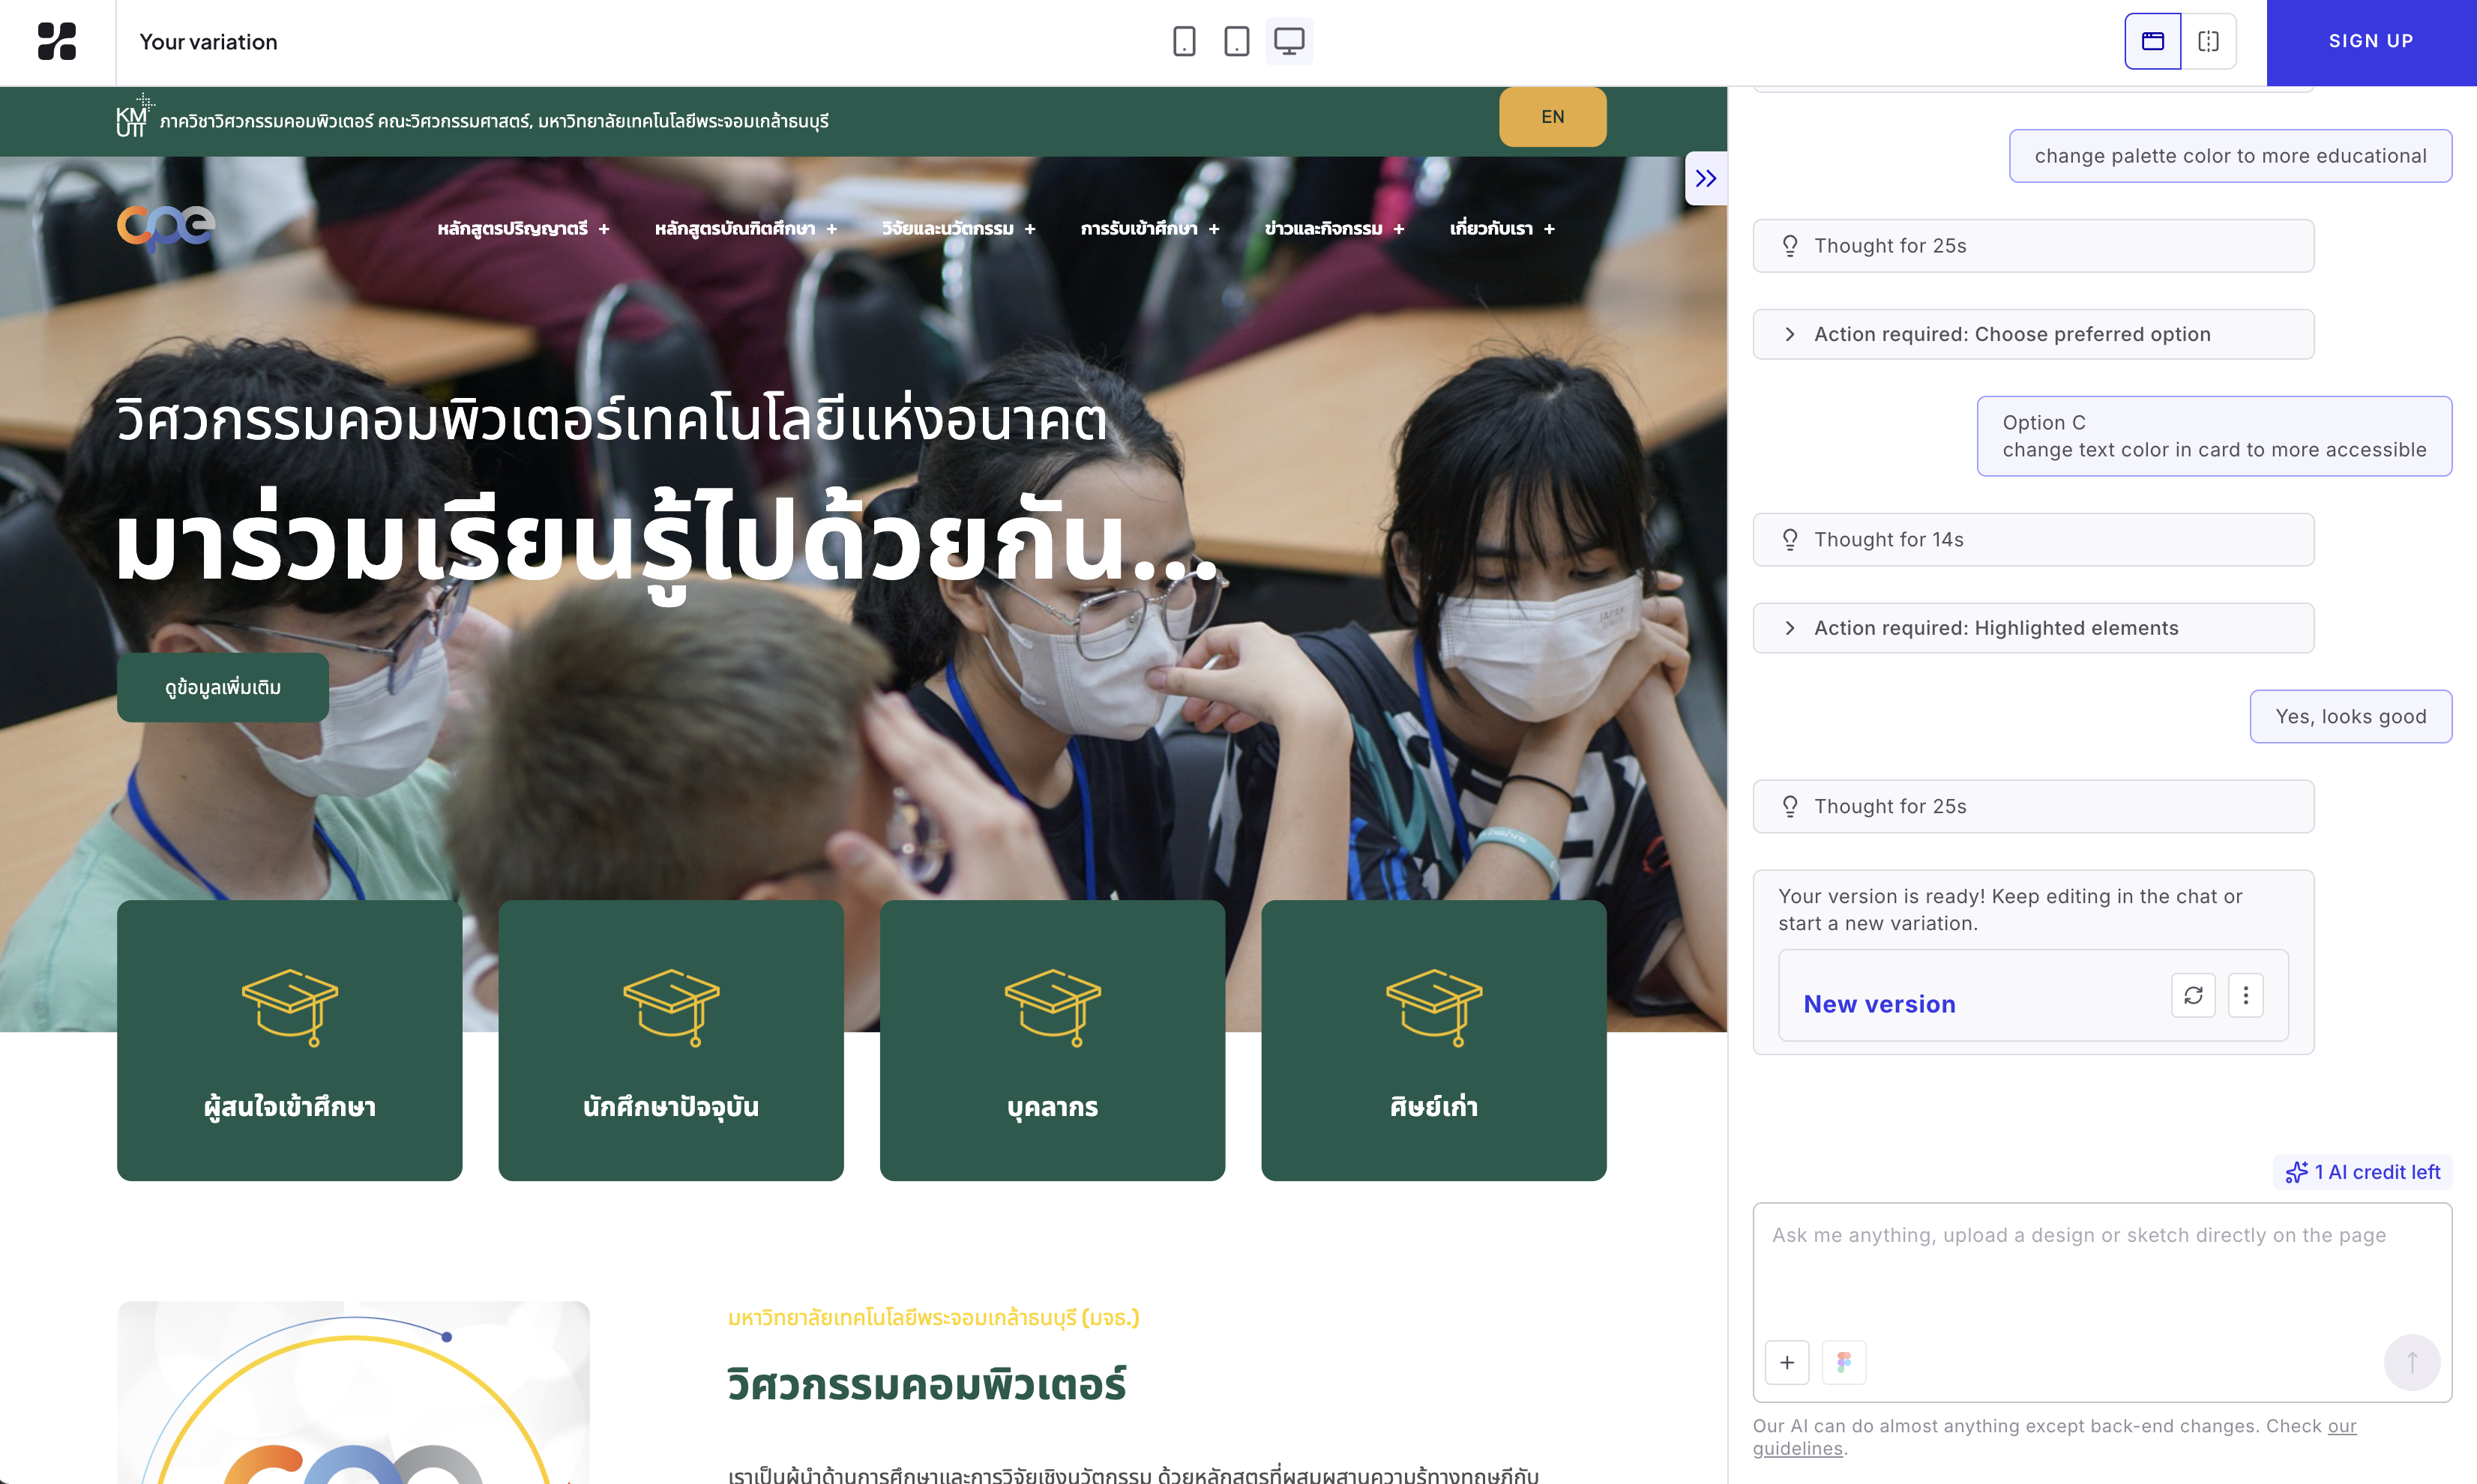
\includegraphics[
          width=0.5\textheight,
          height=0.95\linewidth,
          keepaspectratio,
          origin=c
        ]{figures/ch2-literature-review/kameleoon.png}
        \caption{แพลตฟอร์ม Kameleoon ใช้สำหรับการทำ A/B Testing}
        \label{fig:kameleoon}
      \end{figure}

    \item \textbf{เครื่องมือทดสอบผู้ใช้ก่อนเขียนโค้ด (เช่น Lyssna, Useberry)} มีฟังก์ชัน Preference testing สำหรับเปรียบเทียบดีไซน์หลายแบบ~\cite{lyssna,useberry} และ Lyssna เริ่มมี AI ช่วยสรุปธีมหลักจากคำตอบของผู้เข้าร่วมแล้ว~\cite{lyssna_synthesize} แต่จากการสำรวจเครื่องมือกลุ่มนี้ยังไม่ใช้ AI สร้างทางเลือกการออกแบบ (Variants) และยังไม่แยกปัญหาการใช้งาน (Pain point) ออกจากความชอบของผู้ใช้ในระบบเดียวกัน
      \begin{figure}[H]
        \centering
        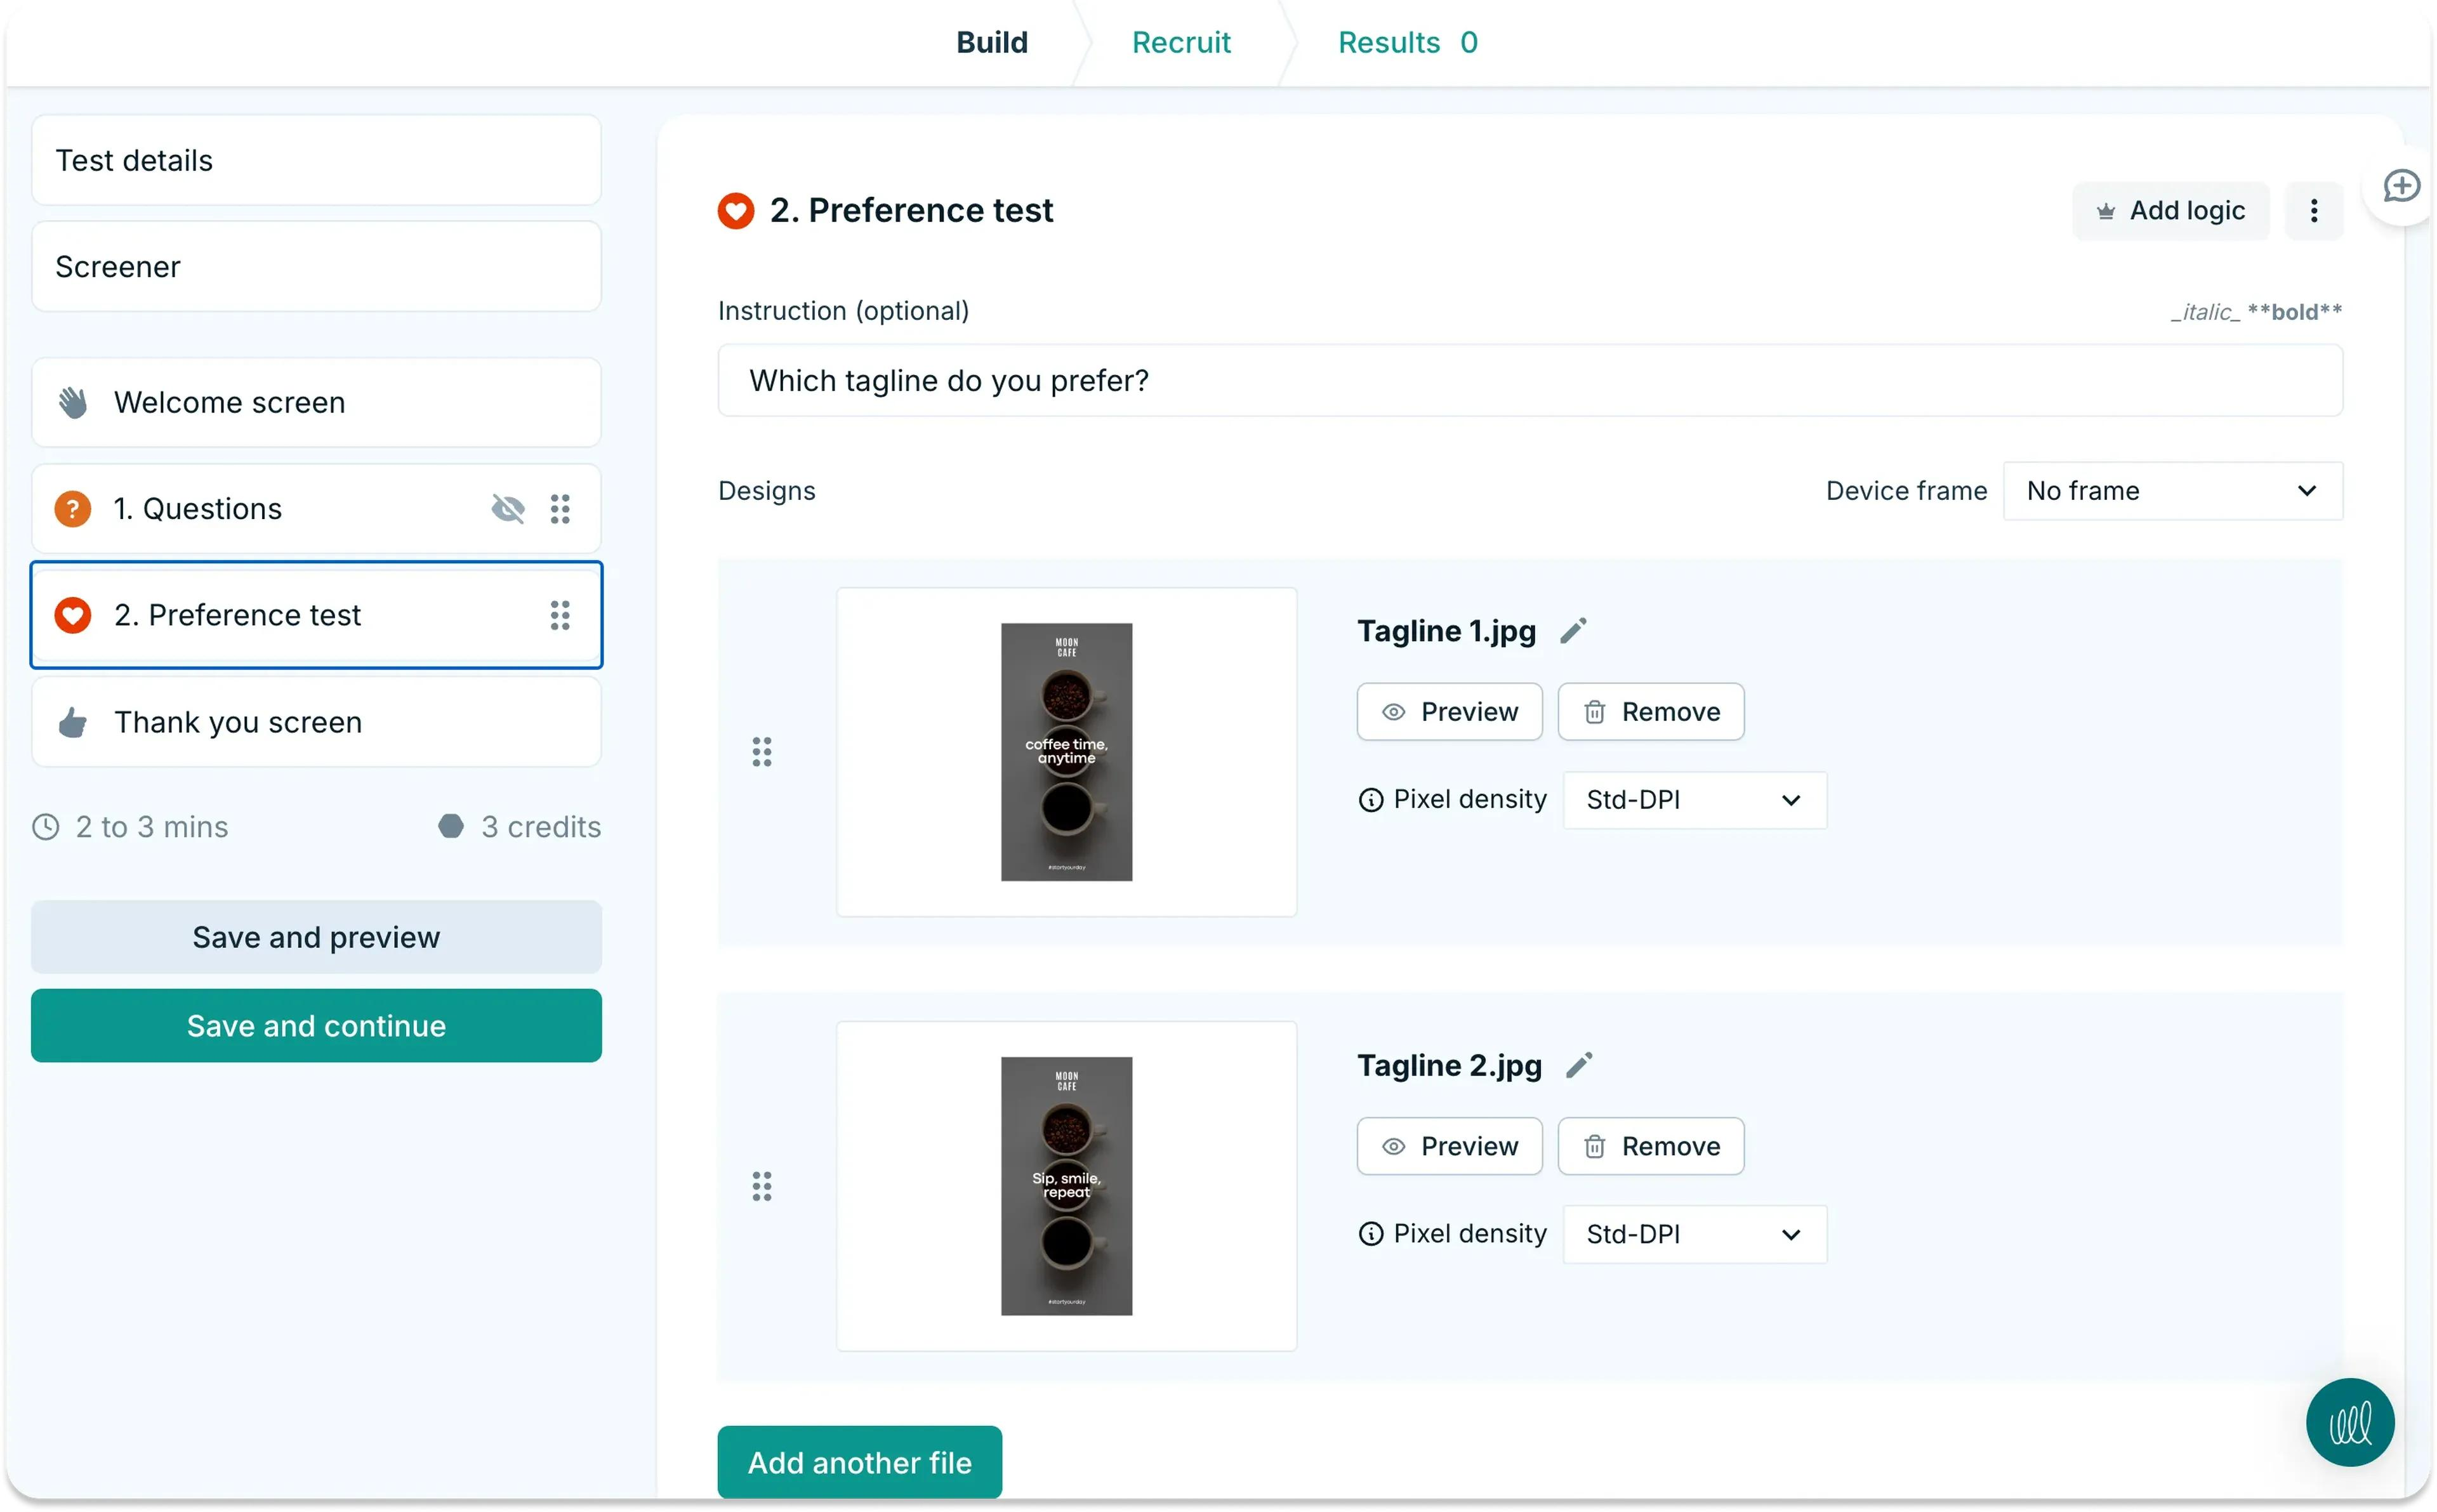
\includegraphics[
          width=0.5\textheight,
          height=0.95\linewidth,
          keepaspectratio,
          origin=c
        ]{figures/ch2-literature-review/lyssna.png}
        \caption{แพลตฟอร์ม Lyssna ใช้สำหรับการทดสอบการใช้งาน}
        \label{fig:lyssna}
      \end{figure}

    \item \textbf{เครื่องมือออกแบบที่มีปัญญาประดิษฐ์เป็นตัวช่วยในการทำงาน (เช่น Figma Make, Figma Agent)} สามารถสร้างต้นแบบหรือ Variants จากคำสั่งได้ โดย agent ของ Figma สร้าง Variants สำหรับ split test จาก component, token และ style ของ Design System~\cite{figma_agent} อย่างไรก็ตาม จากการสำรวจเครื่องมือกลุ่มนี้ยังไม่มีระบบรวบรวมข้อเสนอแนะจากผู้ทดสอบหลายกลุ่มเพื่อนำมาวิเคราะห์ร่วมกัน\cite{figma_agent}
      \begin{figure}[H]
        \centering
        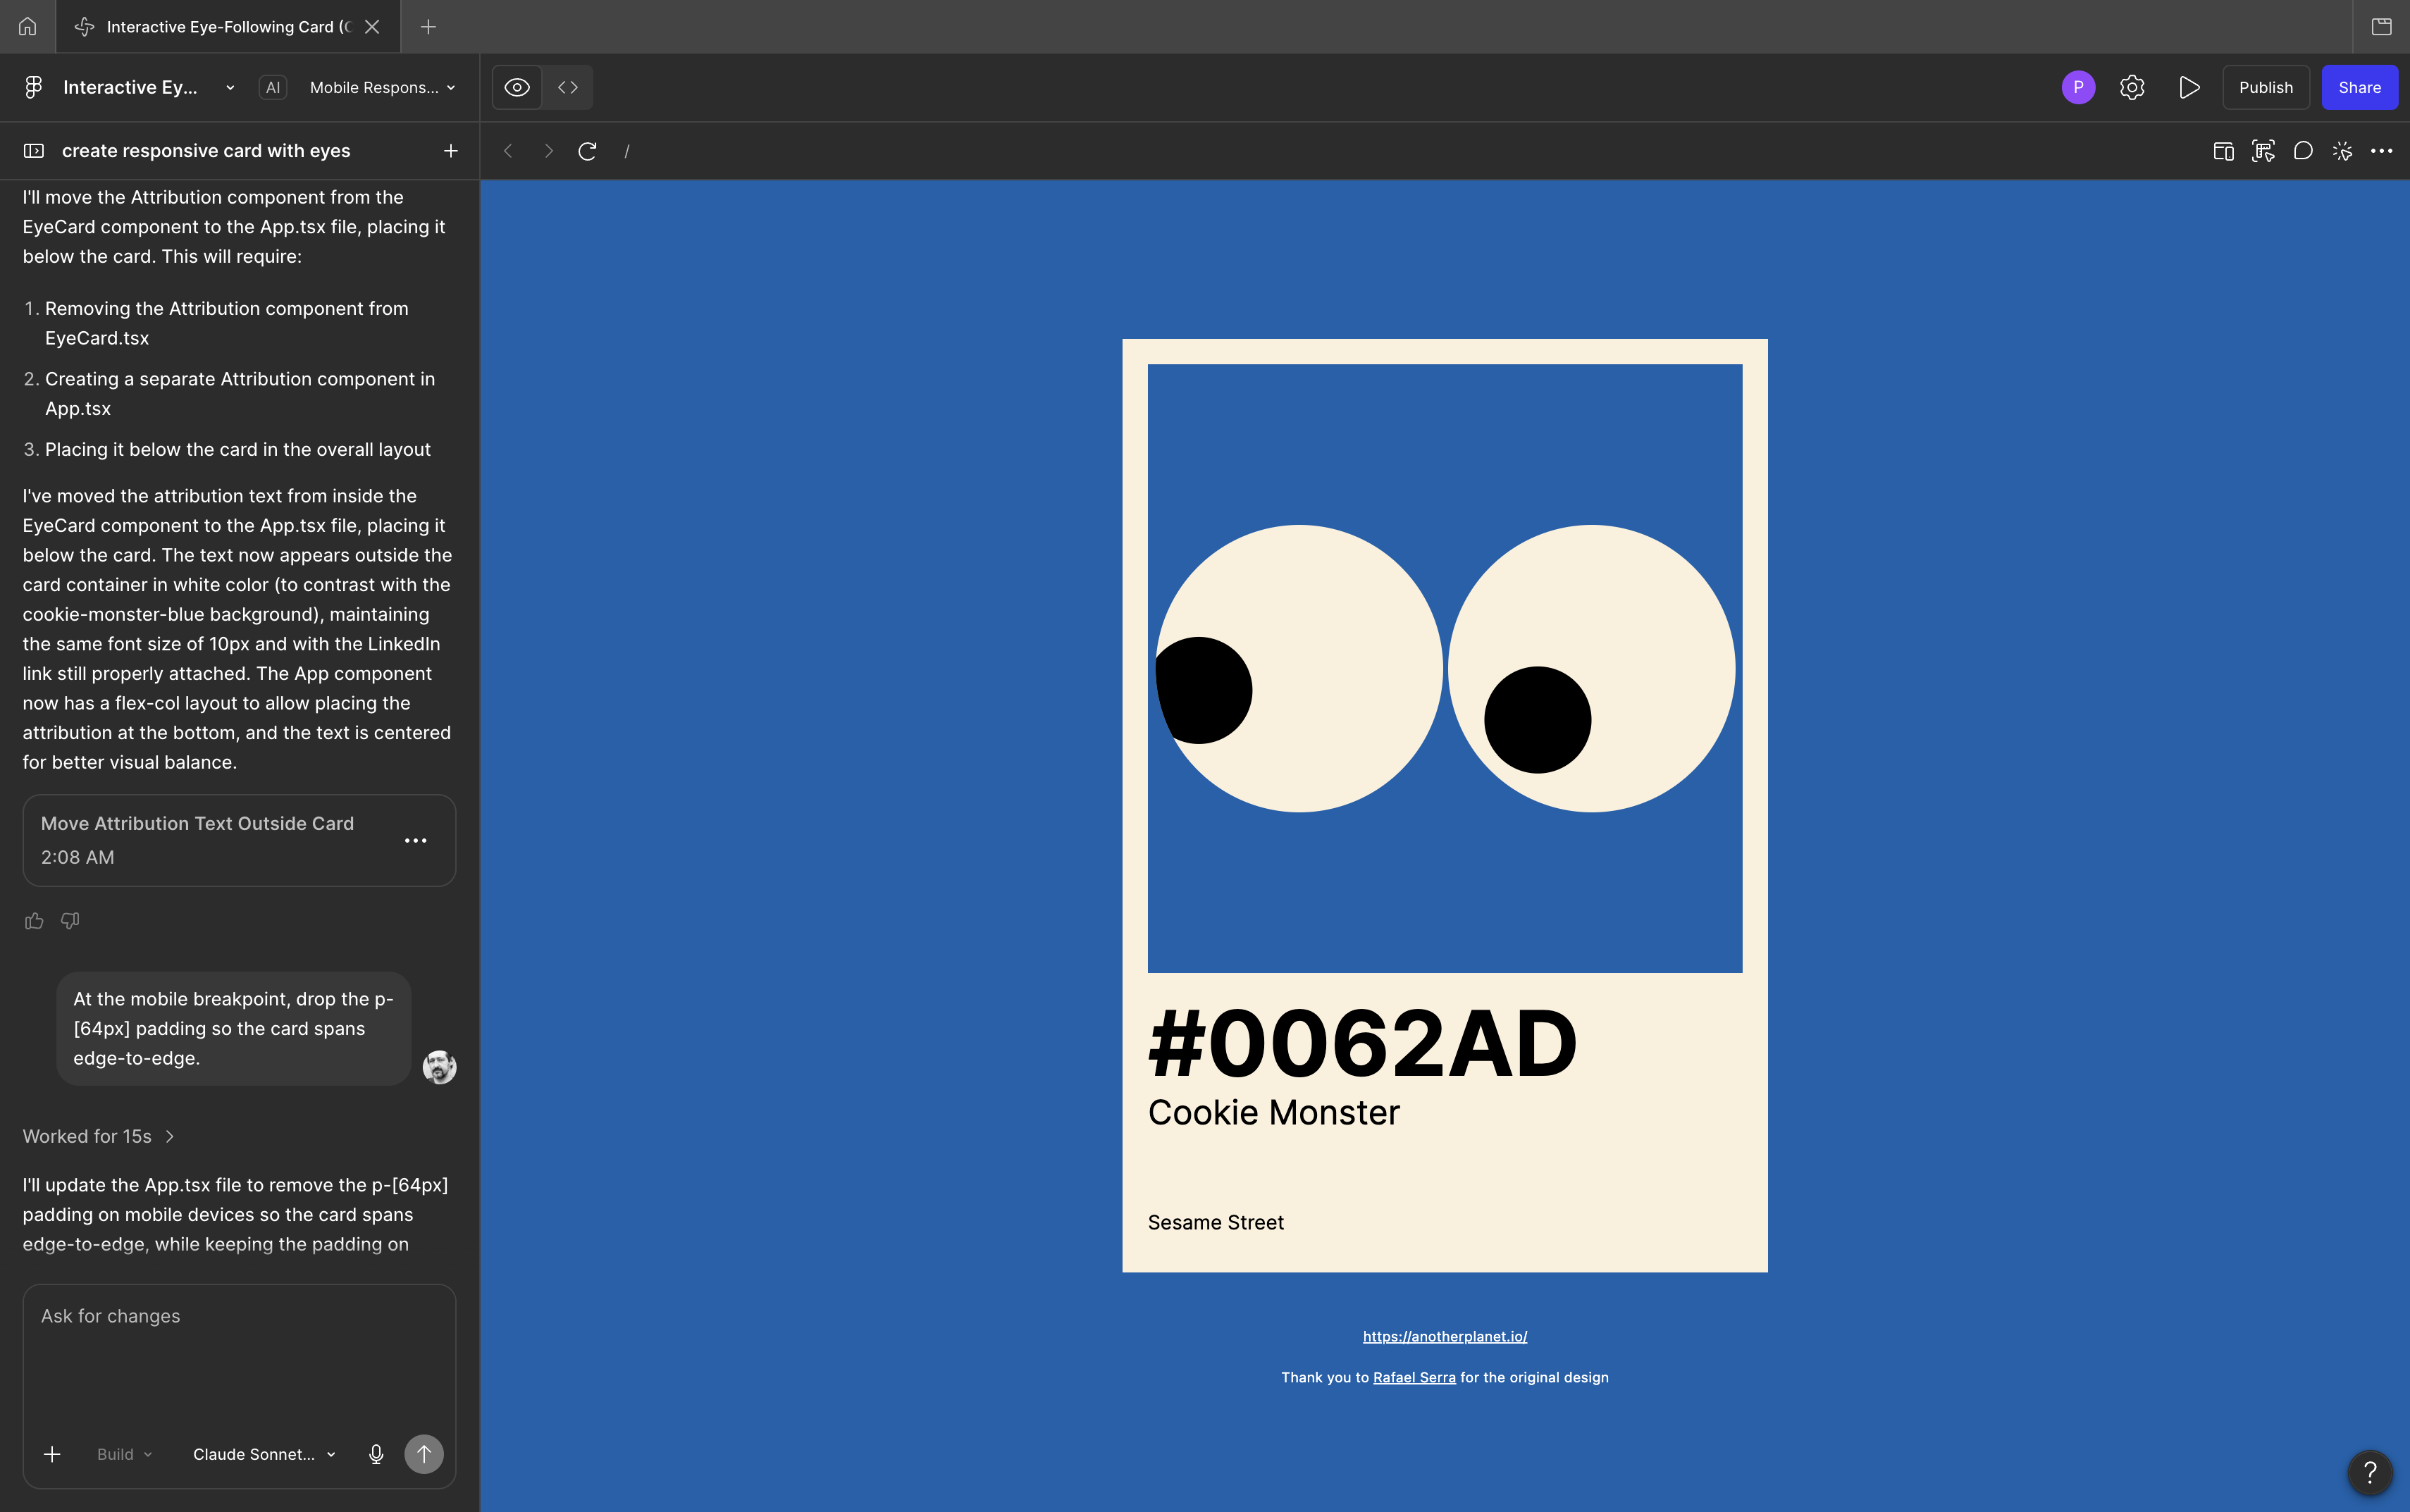
\includegraphics[
          width=0.5\textheight,
          height=0.95\linewidth,
          keepaspectratio,
          origin=c
        ]{figures/ch2-literature-review/figma-make.png}
        \caption{แพลตฟอร์ม Figma Make ใช้สำหรับสร้าง UI ด้วยภาษาธรรมชาติ}
        \label{fig:figma-make}
      \end{figure}

    \item \textbf{เครื่องมือตรวจงานด้วยหมุดคอมเมนต์ (เช่น BugHerd, Marker.io)} ให้ผู้ใช้ปักหมุดความคิดเห็นบนหน้าเว็บ พร้อมแนบภาพหน้าจอและข้อมูลทางเทคนิคโดยอัตโนมัติ~\cite{bugherd,markerio} และเริ่มนำ AI มาใช้จัดการข้อเสนอแนะแล้ว เช่น BugHerd เชื่อมต่อ AI agent ผ่าน MCP เพื่อช่วยคัดแยกงาน~\cite{bugherd_ai} แต่ยังขาดฟังก์ชันเปรียบเทียบสองทางเลือกและการจำแนกข้อเสนอแนะตามประเภทปัญหา
  \end{itemize}
}

% !TeX root = ../../progress-sem1.tex
% 2.x สรุปการศึกษาค้นคว้า
\section{สรุปการศึกษาค้นคว้า}

% \begin{table}[H]
%   \centering
%   \small
%   \caption{สรุปประเด็นจากงานวิจัยและเครื่องมือที่เกี่ยวข้อง}
%   \label{tab:literature_summary}
%   \begin{tabularx}{\textwidth}{
%       >{\raggedright\arraybackslash}p{0.18\textwidth}
%       >{\raggedright\arraybackslash}p{0.22\textwidth}
%       >{\raggedright\arraybackslash}X
%       >{\raggedright\arraybackslash}X
%     }
%     \hline
%     \textbf{กลุ่มประเด็น} &
%     \textbf{งานที่เกี่ยวข้อง} &
%     \textbf{สิ่งที่มีการศึกษาแล้ว} &
%     \textbf{ช่องว่างที่พบ} \\
%     \hline

%     การสร้าง UI และต้นแบบด้วย Generative AI &
%     \cite{suh2025storyensemble, feng2023designing, yuan2024towards, kolthoff2024} &
%     Generative AI สามารถช่วยสร้าง wireframe, prototype และทางเลือกของ UI
%     จากความต้องการของนักออกแบบ เพื่อลดเวลาและแรงงานในการสร้างต้นแบบ
%     และช่วยให้สามารถสำรวจทางเลือกของการออกแบบได้มากขึ้น &
%     ผลลัพธ์ที่สร้างโดย Generative AI ยังพบปัญหาด้าน layout, style และการตีความ
%     function ที่ไม่ตรงกับความต้องการ รวมถึงยังไม่ได้เชื่อมกับกระบวนการ
%     ทดสอบและปรับปรุงจากข้อเสนอแนะของผู้ใช้อย่างครบวงจร \\

%     \hline

%     การทดสอบและการสกัดความต้องการจากต้นแบบ &
%     \cite{nielsen2000five, virzi1992refining,
%     nielsen1993mathematical, pacheco2018, lu2026} &
%     การทดสอบกับผู้ใช้กลุ่มเล็กหลายรอบสามารถช่วยค้นพบปัญหาได้อย่างมีประสิทธิภาพ
%     และการใช้ prototype ช่วยให้นักออกแบบสามารถสกัดความต้องการและรับ
%     ข้อเสนอแนะก่อนพัฒนาระบบจริงได้ &
%     การทำการทดสอบซ้ำหลายรอบยังสร้างภาระในการเตรียมหลายรูปแบบของ UI
%     รวบรวมข้อเสนอแนะ และนำผลจากแต่ละรอบกลับไปปรับปรุงการออกแบบ \\

%     \hline

%     การตีความข้อเสนอแนะและการสร้าง User Persona &
%     \cite{nngroup_satisfaction, nngroup_qualitative,
%     shukla2025, mitchell1997, shin2024} &
%     งานวิจัยแสดงให้เห็นว่าความชอบของผู้ใช้อาจไม่ตรงกับปัญหาการใช้งานจริง
%     และข้อเสนอแนะยังแตกต่างกันตามบทบาทและความต้องการของผู้ให้ข้อมูล
%     นอกจากนี้ LLM สามารถช่วยสรุปข้อมูลเพื่อสร้าง User Persona ได้
%     แต่ยังต้องอาศัยมนุษย์ในการระบุและตรวจสอบลักษณะที่สำคัญของผู้ใช้ &
%     ยังต้องมีกระบวนการเชื่อมโยงข้อเสนอแนะกับกลุ่มผู้ใช้
%     แยกความต้องการและความชอบออกจากกัน และนำข้อมูลเหล่านี้ไปสังเคราะห์
%     เป็น Persona ที่นักออกแบบสามารถตรวจสอบและนำกลับไปใช้ในการออกแบบได้ \\

%     \hline

%     การใช้ปัญญาประดิษฐ์วิเคราะห์ข้อเสนอแนะร่วมกับมนุษย์ &
%     \cite{gao2024collabcoder, gebreegziabher2023patat,
%     song2025, amershi2019, pourasad2025} &
%     LLM สามารถช่วยจัดกลุ่ม สรุป และวิเคราะห์ข้อมูลเชิงคุณภาพได้
%     แต่ยังมีข้อจำกัดด้านอคติและอาจพลาดข้อมูลสำคัญ
%     งานวิจัยจึงสนับสนุนการให้มนุษย์เข้ามาตรวจสอบและตัดสินใจร่วมกับปัญญาประดิษฐ์ &
%     จำเป็นต้องมีกระบวนการที่ให้นักออกแบบตรวจสอบ แก้ไข
%     และยืนยันผลการวิเคราะห์ของปัญญาประดิษฐ์ก่อนที่ผลลัพธ์จะถูกนำไปใช้
%     ปรับปรุงงานออกแบบ \\

%     \hline

%     เครื่องมือที่มีอยู่ในปัจจุบัน &
%     \cite{kameleoon, otterab, lyssna, useberry,
%     figma_agent, bugherd, markerio} &
%     เครื่องมือแต่ละประเภทสนับสนุนบางส่วนของกระบวนการ เช่น
%     การทดสอบหลายรูปแบบ การทดสอบ prototype การสร้าง UI ด้วย AI
%     หรือการให้ข้อเสนอแนะบนงานออกแบบ &
%     ความสามารถเหล่านี้ยังแยกอยู่ในหลายเครื่องมือ
%     และยังไม่มีการเชื่อมตั้งแต่การสร้างทางเลือกของ UI
%     การทดสอบ การวิเคราะห์ข้อเสนอแนะ การสร้าง Persona
%     จนถึงการนำผลกลับไปใช้ในรอบการออกแบบถัดไป \\

%     \hline
%   \end{tabularx}
% \end{table}

\thaijustify{
  จากการศึกษางานวิจัยและเครื่องมือที่เกี่ยวข้อง พบว่าแต่ละแนวทางสามารถสนับสนุนบางส่วนของ UX/UI DLC ได้แล้ว แต่กระบวนการตั้งแต่
  การสร้างต้นแบบ การทดสอบกับผู้ใช้ การรวบรวมและวิเคราะห์ข้อเสนอแนะจนถึงการนำข้อมูลกลับไปปรับปรุงการออกแบบยังคงแยกออกจากกัน
}
\thaijustify{
  ดังนั้น โครงงานนี้จึงมุ่งเชื่อมกระบวนการเหล่านี้เข้าด้วยกันโดยใช้ Generative AI ช่วยสร้าง two-alternative UI จากความต้องการทางการออกแบบ แล้วนำไปทำ Comparative Usability Test และให้ผู้เข้าร่วมทดสอบสามารถให้ข้อเสนอแนะลงบน component ได้โดยตรง จากนั้นระบบจะช่วยรวบรวมและวิเคราะห์ข้อเสนอแนะเพื่อค้นหาปัญหา ความต้องการ ความชอบและลักษณะร่วมของผู้ใช้แต่ละกลุ่ม เพื่อนำไปสนับสนุนการสร้าง Persona Artifact โดยให้นักออกแบบเป็นผู้ตรวจสอบและตัดสินใจผลลัพธ์ก่อนนำข้อมูลที่ผ่านการยืนยันแล้วกลับไปใช้ในการสร้างและทดสอบรอบถัดไป
}
\thaijustify{
  แนวทางดังกล่าวทำให้ โครงงานไม่ได้มุ่งใช้ Generative AI เพื่อสร้าง two-alternative UI เพียงอย่างเดียว แต่ใช้ปัญญาประดิษฐ์เพื่อสนับสนุน UX/UI DLC ตั้งแต่การสร้างต้นแบบ การทดสอบการใช้งาน ไปจนถึงการนำความต้องการ
  ของผู้ใช้กลับมาใช้ในการตัดสินใจเชิงออกแบบ โดยยังคงให้นักออกแบบเป็นผู้ควบคุมการตัดสินใจในแต่ละรอบ
}

% \thaijustify{
%   และจากการทบทวนวรรณกรรมทำให้เห็นช่องว่างทางการวิจัย คือ ปัจจุบันยังไม่มีเครื่องมือหรืองานวิจัยใดที่รวบรวมความสามารถทั้ง 4 ด้านไว้ในระบบเดียว ได้แก่ (1) การใช้ปัญญาประดิษฐ์สร้าง two-alternative UI ภายใต้ Design system ที่กำหนด (2) การให้ผู้ทดสอบให้ข้อเสนอแนะ (3) การใช้ปัญญาประดิษฐ์แยกแยะ pain point ออกจากความชอบร่วมกับการตัดสินใจของนักออกแบบ และ (4) การสร้าง Persona Artifact จากผลลัพธ์
% }
% \thaijustify{สิ่งที่โครงงานนี้ควรให้ความสำคัญเป็น คือ การพัฒนาแพลตฟอร์มนี้ให้ครอบคลุมกระบวนการตั้งแต่รับโจทย์ สร้างต้นแบบ รวบรวมข้อเสนอแนะ และวิเคราะห์ผลลัพธ์ เพื่อให้นักออกแบบสามารถส่งมอบงานที่มีการตรวจสอบความต้องการของผู้ใช้ที่แท้จริง พร้อมด้วย design system และต้นแบบที่ลูกค้าพึงพอใจให้นักพัฒนาต่อไปได้อย่างมีประสิทธิภาพ
% }


%%%%%%%%%%%%%%%%%%%%%%%%%%%%%%%%% Chapter 3 %%%%%%%%%%%%%%%%%%%%%%%%%%%%%
\chapter{การออกแบบและวิธีการดำเนินงาน}
% !TeX root = ../../progress-sem1.tex
% Chapter 3 opening paragraph (uses \termphrase from the entry file)
\thaijustify{
  ในบทที่ 3 จะกล่าวถึงการสำรวจและวิเคราะห์ความต้องการของระบบ การออกแบบระบบ สถาปัตยกรรมโดยภาพรวม การออกแบบส่วนต่อประสานผู้ใช้ การพัฒนา AI pipeline และการพัฒนาระบบที่ดำเนินการ\termphrase
}

% !TeX root = ../../progress-sem1.tex
% 3.x การสำรวจและวิเคราะห์ความต้องการของระบบ
\section{การสำรวจและวิเคราะห์ความต้องการของระบบ}
\subsection{การสัมภาษณ์ผู้มีส่วนได้ส่วนเสีย}
\thaijustify{
  \todo{กลุ่มที่สัมภาษณ์ จำนวนผู้ให้สัมภาษณ์ วิธีการ และข้อค้นพบหลัก}
}
\subsection{ข้อค้นพบและความต้องการที่ได้จากการสัมภาษณ์}
\thaijustify{
  \todo{สรุป pain point และความต้องการที่นำมากำหนด requirement}
}

% !TeX root = ../../progress-sem1.tex
% 3.x ความต้องการของระบบ (functional / non-functional requirements)
\section{ความต้องการของระบบ}\label{sec:requirements}
\thaijustify{
  ความต้องการของระบบกำหนดจากวัตถุประสงค์และขอบเขตของโครงงานในบทที่ 1 แผนภาพกรณีการใช้งาน และหน้าจอ high-fidelity ที่ออกแบบไว้ แบ่งเป็นความต้องการเชิงฟังก์ชันและความต้องการที่ไม่ใช่เชิงฟังก์ชัน
}
\subsection{Functional Requirements}
\thaijustify{
  ความต้องการเชิงฟังก์ชันแบ่งตามส่วนของระบบ แสดงในตารางที่~\ref{tab:functional-requirements} โดยเครื่องหมาย \checkmark{} ระบุบทบาทที่ใช้งานความต้องการนั้น
}
\begingroup
\small
\newcommand{\rot}[1]{\rotatebox{90}{\textbf{#1}\,}}
\begin{xltabular}{\linewidth}{|>{\RaggedRight\arraybackslash}p{0.1\linewidth}|>{\RaggedRight\arraybackslash}X|*{5}{>{\centering\arraybackslash}m{0.045\linewidth}|}}
  \caption{Functional requirements และบทบาทที่ใช้งาน}\label{tab:functional-requirements}\\
  \hline
  \textbf{รหัส} & \textbf{ความต้องการ} & \rot{Designer} & \rot{Tester} & \rot{Client} & \rot{Developer} & \rot{PM} \\ \hline
  \endfirsthead
  \multicolumn{7}{l}{\textit{ตารางที่ \thetable\ (ต่อ)}}\\
  \hline
  \textbf{รหัส} & \textbf{ความต้องการ} & \rot{Designer} & \rot{Tester} & \rot{Client} & \rot{Developer} & \rot{PM} \\ \hline
  \endhead
  \multicolumn{7}{|l|}{\textbf{การยืนยันตัวตนและสิทธิ์}} \\ \hline
  FR-01 & ผู้ใช้สมัครสมาชิกและเข้าสู่ระบบด้วยบัญชี Google หรืออีเมลและรหัสผ่านได้ โดยบัญชีที่สมัครด้วยอีเมลต้องยืนยันอีเมลก่อนใช้งาน & \checkmark &  & \checkmark & \checkmark & \checkmark \\ \hline
  FR-02 & ผู้ใช้รีเซ็ตรหัสผ่านผ่านลิงก์ที่ส่งทางอีเมลได้ & \checkmark &  & \checkmark & \checkmark & \checkmark \\ \hline
  FR-03 & ระบบจำกัดการเข้าถึงข้อมูลและการกระทำตามบทบาทของผู้ใช้ในแต่ละโปรเจกต์ & \checkmark &  & \checkmark & \checkmark & \checkmark \\ \hline
  \multicolumn{7}{|l|}{\textbf{การตั้งค่าโปรเจกต์}} \\ \hline
  FR-04 & ผู้ใช้สร้าง workspace เชิญสมาชิกด้วยอีเมลหรือลิงก์ และสลับระหว่าง workspace ได้ & \checkmark &  &  &  &  \\ \hline
  FR-05 & Designer สร้าง แก้ไข และค้นหาโปรเจกต์ พร้อมกำหนดสมาชิกและบทบาทในโปรเจกต์ได้ & \checkmark &  &  &  &  \\ \hline
  FR-06 & Designer กำหนด design intent ได้แก่ persona, design system, มาตรฐานการเข้าถึง, สีแบรนด์, แนวทาง CI และ tone of voice & \checkmark &  &  &  &  \\ \hline
  \multicolumn{7}{|l|}{\textbf{การสร้าง UI ด้วย AI}} \\ \hline
  FR-07 & Designer เขียน user story, problem statement, ตัวชี้วัดความสำเร็จ และเลือกอุปกรณ์ที่ต้องการทดสอบได้ & \checkmark &  &  &  &  \\ \hline
  FR-08 & ระบบใช้ AI ร่าง structured prompt จาก design intent, persona และ user story ให้ Designer ตรวจและแก้ไขก่อนสร้าง UI & \checkmark &  &  &  &  \\ \hline
  FR-09 & ระบบสร้าง two-alternative UI ตาม prompt ที่อนุมัติ โดยใช้ component ของ design system ที่เลือก และแสดงความคืบหน้าแบบ real-time & \checkmark &  &  &  &  \\ \hline
  FR-10 & Designer ปรับแก้ UI ผ่านแชตหรือเลือก element บนหน้าจอ ดูหน้าจอในขนาดอุปกรณ์ต่าง ๆ และย้อนดูเวอร์ชันก่อนหน้าได้ & \checkmark &  &  &  &  \\ \hline
  \multicolumn{7}{|l|}{\textbf{การทดสอบ}} \\ \hline
  FR-11 & Designer กำหนดภารกิจ คำถามเปรียบเทียบ คำถามเฉพาะจุด จำนวนผู้เข้าร่วมทดสอบ และเงื่อนไขการหยุดทดสอบได้ & \checkmark &  &  &  &  \\ \hline
  FR-12 & ระบบสร้างรหัสหรือลิงก์สำหรับเข้าเซสชันการทดสอบ ผู้เข้าร่วมทดสอบเข้าได้โดยไม่ต้องมีบัญชี & \checkmark & \checkmark &  &  &  \\ \hline
  FR-13 & ผู้เข้าร่วมทดสอบต้องให้ความยินยอมตาม PDPA ก่อนเริ่มทดสอบ &  & \checkmark &  &  &  \\ \hline
  FR-14 & ผู้เข้าร่วมทดสอบทำภารกิจบนทั้งสองดีไซน์ ตอบคำถามผ่านแชต และให้ความเห็นต่อ component หรือทั้งหน้าจอได้ &  & \checkmark &  &  &  \\ \hline
  \multicolumn{7}{|l|}{\textbf{การวิเคราะห์ข้อเสนอแนะ}} \\ \hline
  FR-15 & Designer ติดตามความคืบหน้าและแนวโน้มความคิดเห็นของผู้เข้าร่วมทดสอบแต่ละคน และเข้าไปกำหนดทิศทางเมื่อแนวโน้มผิดปกติได้ & \checkmark &  &  &  &  \\ \hline
  FR-16 & ระบบใช้ AI จัดกลุ่มข้อเสนอแนะเป็นประเด็น ให้ Designer ปรับป้ายกำกับ รวม แยก หรือระบุว่าไม่แก้ไขพร้อมเหตุผล & \checkmark &  &  &  &  \\ \hline
  FR-17 & Designer เลือกประเด็นที่ต้องการแก้ไข แล้วระบบสร้าง UI สำหรับรอบถัดไป โดยบันทึกความเชื่อมโยงระหว่างข้อเสนอแนะกับการเปลี่ยนแปลง & \checkmark &  &  &  &  \\ \hline
  FR-18 & ระบบสร้าง Persona Artifact จากประเด็นที่ Designer ยืนยันแล้ว & \checkmark &  &  &  &  \\ \hline
  \multicolumn{7}{|l|}{\textbf{รายงาน}} \\ \hline
  FR-19 & ระบบสร้างรายงานแยกตามบทบาทจากรอบที่อนุมัติแล้ว ให้ Designer แก้ไขก่อนเผยแพร่ & \checkmark &  &  &  &  \\ \hline
  FR-20 & Client, Developer และ Project Manager ดูรายงานของบทบาทตนเอง รับทราบและแสดงความเห็นได้ &  &  & \checkmark & \checkmark & \checkmark \\ \hline
  FR-21 & ผู้ใช้ส่งออกรายงานเป็น PDF หรือแชร์เป็นลิงก์ได้ & \checkmark &  & \checkmark & \checkmark & \checkmark \\ \hline
\end{xltabular}
\endgroup

\subsection{Non-Functional Requirements}
\thaijustify{
  ความต้องการที่ไม่ใช่เชิงฟังก์ชันแสดงในตารางที่~\ref{tab:non-functional-requirements}
}
\begingroup
\small
\begin{xltabular}{\linewidth}{|>{\RaggedRight\arraybackslash}p{0.11\linewidth}|>{\RaggedRight\arraybackslash}p{0.2\linewidth}|>{\RaggedRight\arraybackslash}X|}
  \caption{Non-functional requirements}\label{tab:non-functional-requirements}\\
  \hline
  \textbf{รหัส} & \textbf{ด้าน} & \textbf{ความต้องการ} \\ \hline
  \endfirsthead
  \multicolumn{3}{l}{\textit{ตารางที่ \thetable\ (ต่อ)}}\\
  \hline
  \textbf{รหัส} & \textbf{ด้าน} & \textbf{ความต้องการ} \\ \hline
  \endhead
  NFR-01 & ความปลอดภัย & ใช้ access token แบบ JWT ที่มีอายุสั้น และ refresh token ที่เก็บเป็นค่า hash และเปลี่ยนใหม่ทุกครั้งที่ใช้ ตรวจสิทธิ์ทุก API ตาม permission ของบทบาท และบันทึกการกระทำสำคัญลง audit log \\ \hline
  NFR-02 & ความเป็นส่วนตัว (PDPA) & เก็บความยินยอมของผู้เข้าร่วมทดสอบพร้อมเวอร์ชันของข้อความ ลบอีเมล หมายเลขโทรศัพท์ และลิงก์ออกจากข้อความก่อนส่งให้ AI และไม่แสดงอีเมลของผู้เข้าร่วมทดสอบในหน้าข้อเสนอแนะ \\ \hline
  NFR-03 & การตอบสนอง & งานที่ใช้เวลานาน เช่น การสร้าง UI ทำงานเบื้องหลังผ่านคิว ไม่ทำให้หน้าจอค้าง และแสดงความคืบหน้าแบบ real-time ผ่าน SSE โดยผู้ใช้ยกเลิกงานได้ \\ \hline
  NFR-04 & ความน่าเชื่อถือของผลลัพธ์ AI & ผลลัพธ์ของ AI ต้องอยู่ในรูปแบบที่กำหนด (JSON ตาม schema หรือ HTML) และ UI ที่สร้างต้องผ่านการตรวจ design system, สีแบรนด์ และการเข้าถึงก่อนแสดงให้ Designer \\ \hline
  NFR-05 & การเข้าถึง (Accessibility) & UI ที่ AI สร้างต้องเป็นไปตามมาตรฐานการเข้าถึงที่กำหนดใน design intent ซึ่งค่าเริ่มต้นคือ WCAG 2.1 ระดับ AA \\ \hline
  NFR-06 & การใช้งาน (Usability) & หน้าจอของแพลตฟอร์มใช้ design system เดียวกันทั้งระบบ และผู้เข้าร่วมทดสอบใช้งานได้โดยไม่ต้องสมัครสมาชิกหรือติดตั้งโปรแกรม \\ \hline
  NFR-07 & ความเข้ากันได้ & ใช้งานผ่านเว็บเบราว์เซอร์รุ่นปัจจุบัน และ UI ที่สร้างรองรับการแสดงผลบน desktop, tablet และ mobile \\ \hline
  NFR-08 & การบำรุงรักษา & เปลี่ยนโมเดล AI ได้ผ่านการตั้งค่าโดยไม่ต้องแก้โค้ด ทุก pull request ผ่าน lint และ build อัตโนมัติ และการเปลี่ยน schema ของฐานข้อมูลทำผ่าน migration \\ \hline
  NFR-09 & การตรวจสอบย้อนกลับ & ทุกการตัดสินใจของ Designer และทุกการเปลี่ยนแปลงระหว่างรอบต้องสืบย้อนกลับไปยังข้อเสนอแนะต้นทางได้ \\ \hline
\end{xltabular}
\endgroup

% !TeX root = ../../progress-sem1.tex
% 3.x การออกแบบระบบ (System Design)
\section{การออกแบบระบบ (System Design)}
\begin{samepage}
  \subsection{Use Case Diagram}
  \thaijustify{
    แผนภาพกรณีการใช้งาน (Use case diagram) แสดงความสัมพันธ์ระหว่างผู้ใช้งานแต่ละบทบาทกับฟังก์ชันของแพลตฟอร์ม โดยแบ่งออกเป็น 4 ส่วน ได้แก่ ส่วน Authentication, ส่วนสร้าง two-alternative UI, ส่วนทดสอบการใช้งานและรับความเห็น, และส่วนสร้างรายงาน
  }
  \subsubsection{Authentication}
  \begin{figure}[H]
    \centering
    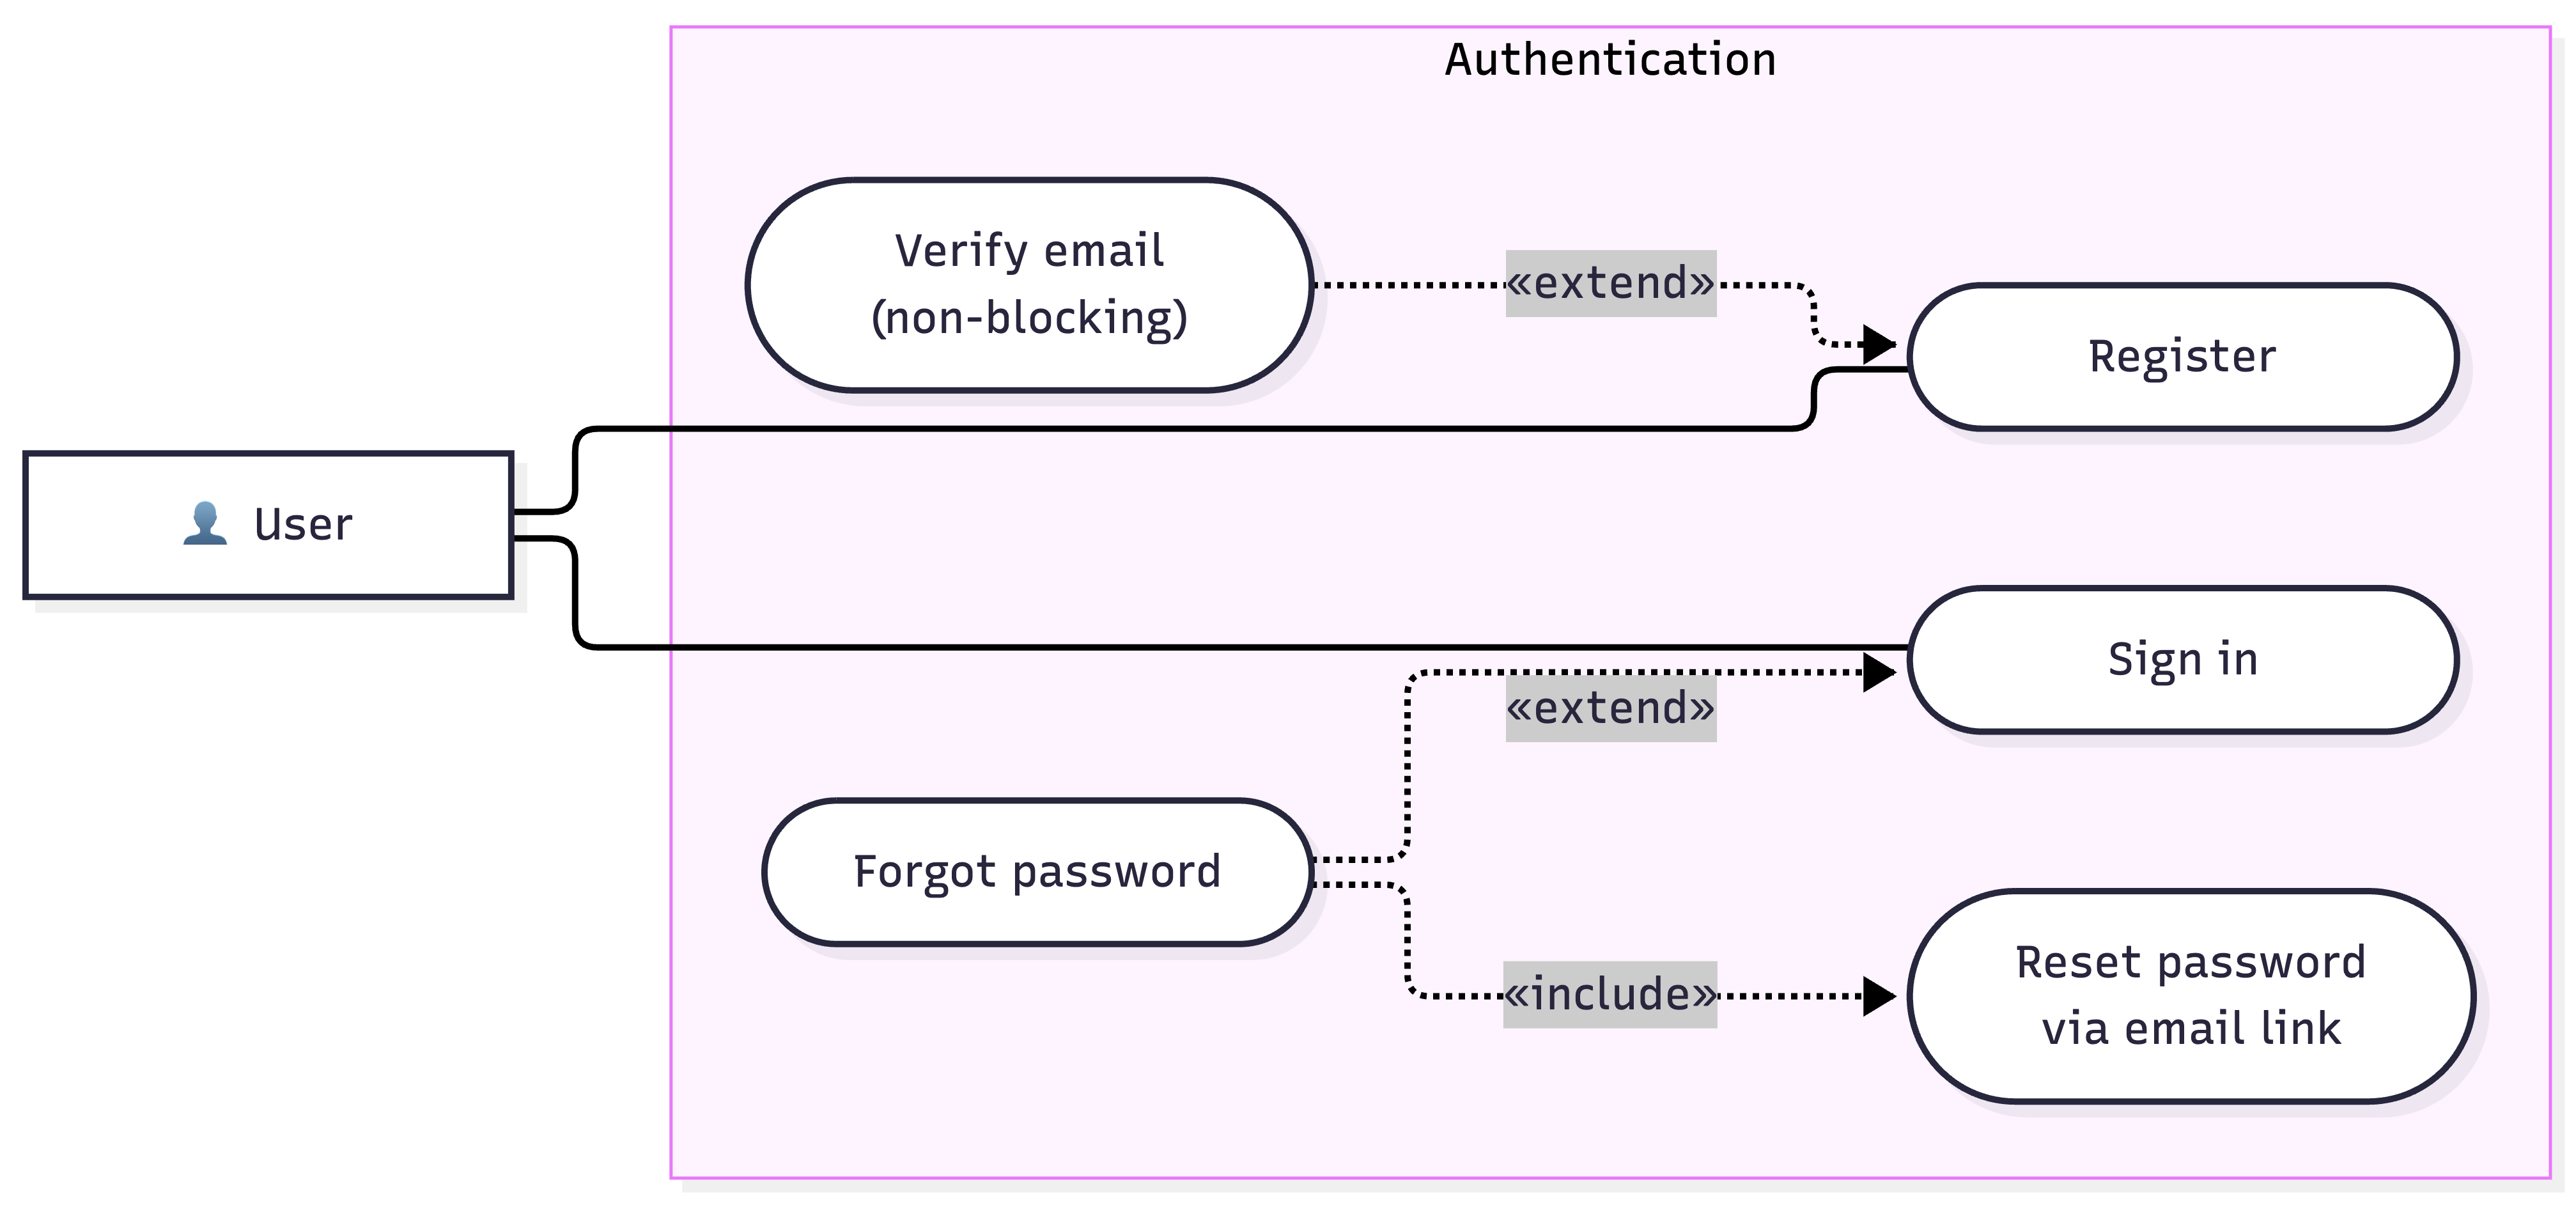
\includegraphics[
      width=0.6\textheight,
      height=\linewidth,
      keepaspectratio,
      origin=c
    ]{figures/ch3-methodology/UC-1.png}
    \caption{Use case diagram for authentication}
    \label{fig:UC-1}
    \thaijustify{ภาพแสดง Use Case ของระบบ Authentication โดยผู้ใช้สามารถสมัครสมาชิก เข้าสู่ระบบ และกู้คืนรหัสผ่านได้ โดยการยืนยันอีเมลเป็นขั้นตอนเสริมหลังการสมัคร และการรีเซ็ตรหัสผ่านดำเนินการผ่านลิงก์ที่ส่งทางอีเมล}
  \end{figure}
  \subsubsection{Designer: Project setup \& UI Generation}
  \begin{figure}[H]
    \centering
    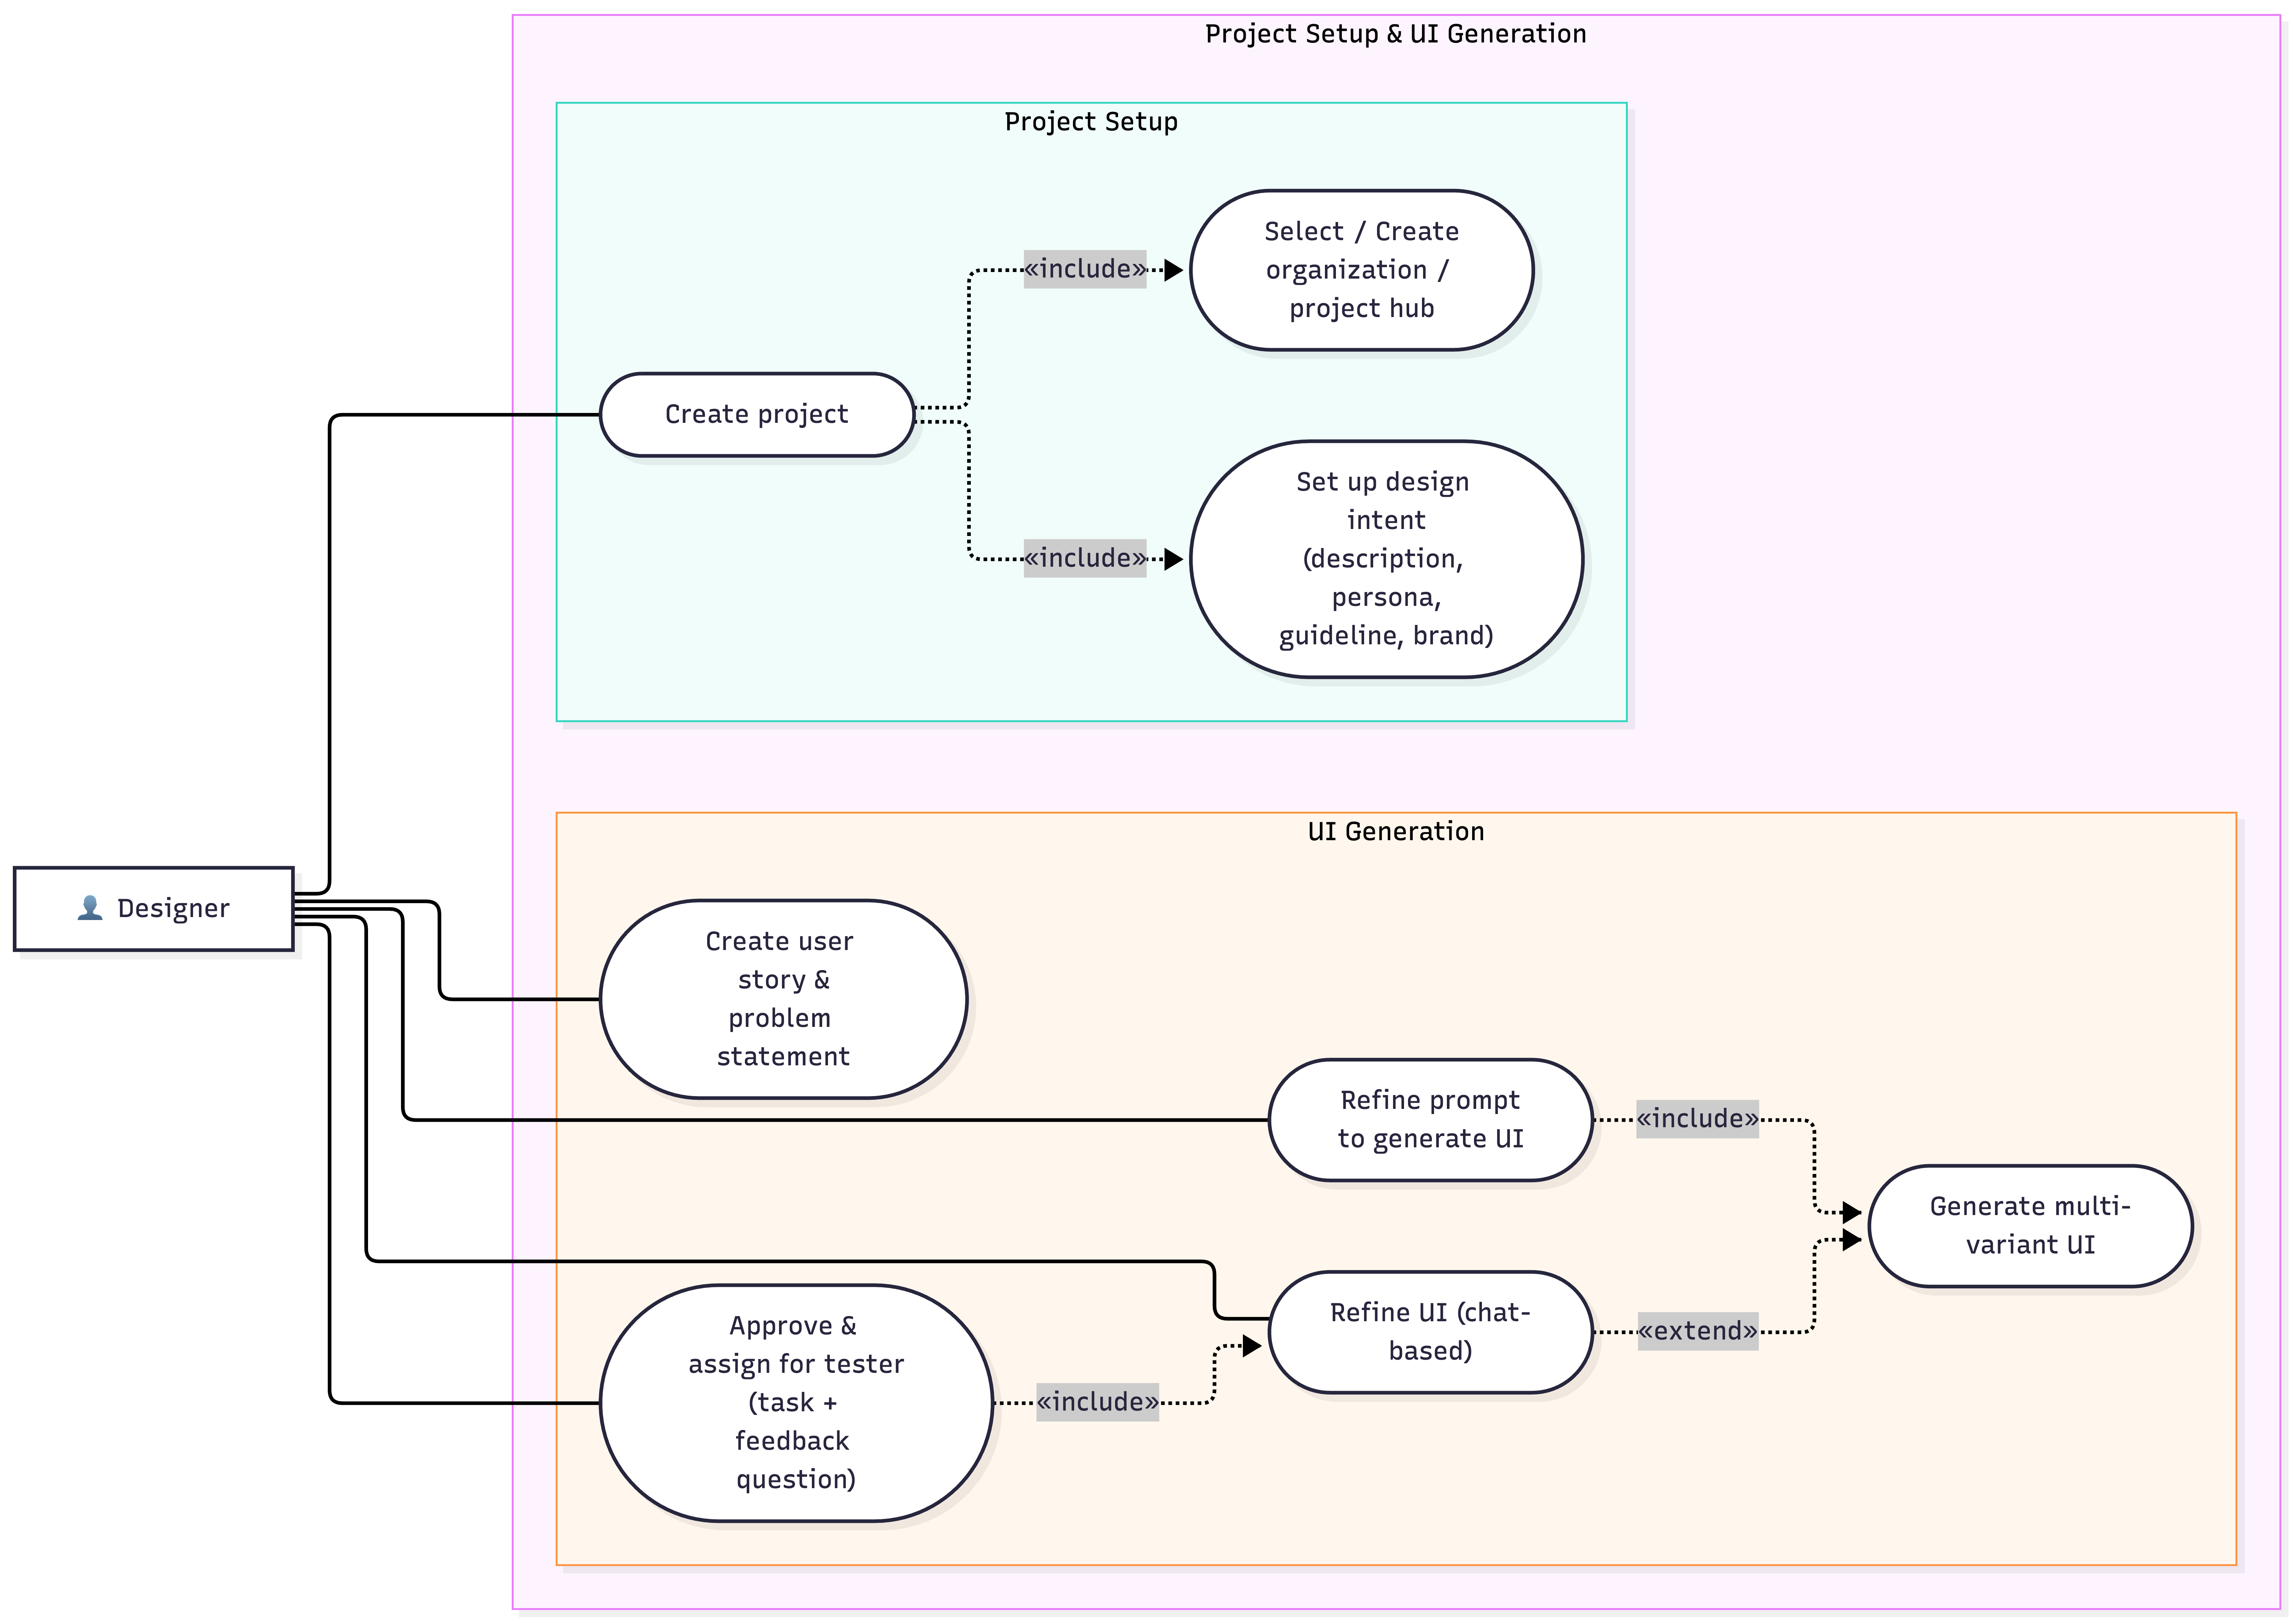
\includegraphics[
      width=0.6\textheight,
      height=\linewidth,
      keepaspectratio,
      origin=c
    ]{figures/ch3-methodology/UC-2.png}
    \caption{Use case diagram for Project setup and UI Generation}
    \label{fig:UC-2}
    \thaijustify{ภาพแสดง Use Case ของกระบวนการจัดเตรียมโครงการและสร้าง UI โดย Designer สามารถสร้างโครงการ กำหนด Design Intent สร้างและปรับแต่ง Prompt เพื่อสร้าง UI หลายรูปแบบ รวมถึงปรับแก้ UI และอนุมัติเพื่อส่งให้ผู้ทดสอบประเมิน}
  \end{figure}
  \subsubsection{Designer and Tester: Testing session and Feedback analysis}
  \begin{figure}[H]
    \centering
    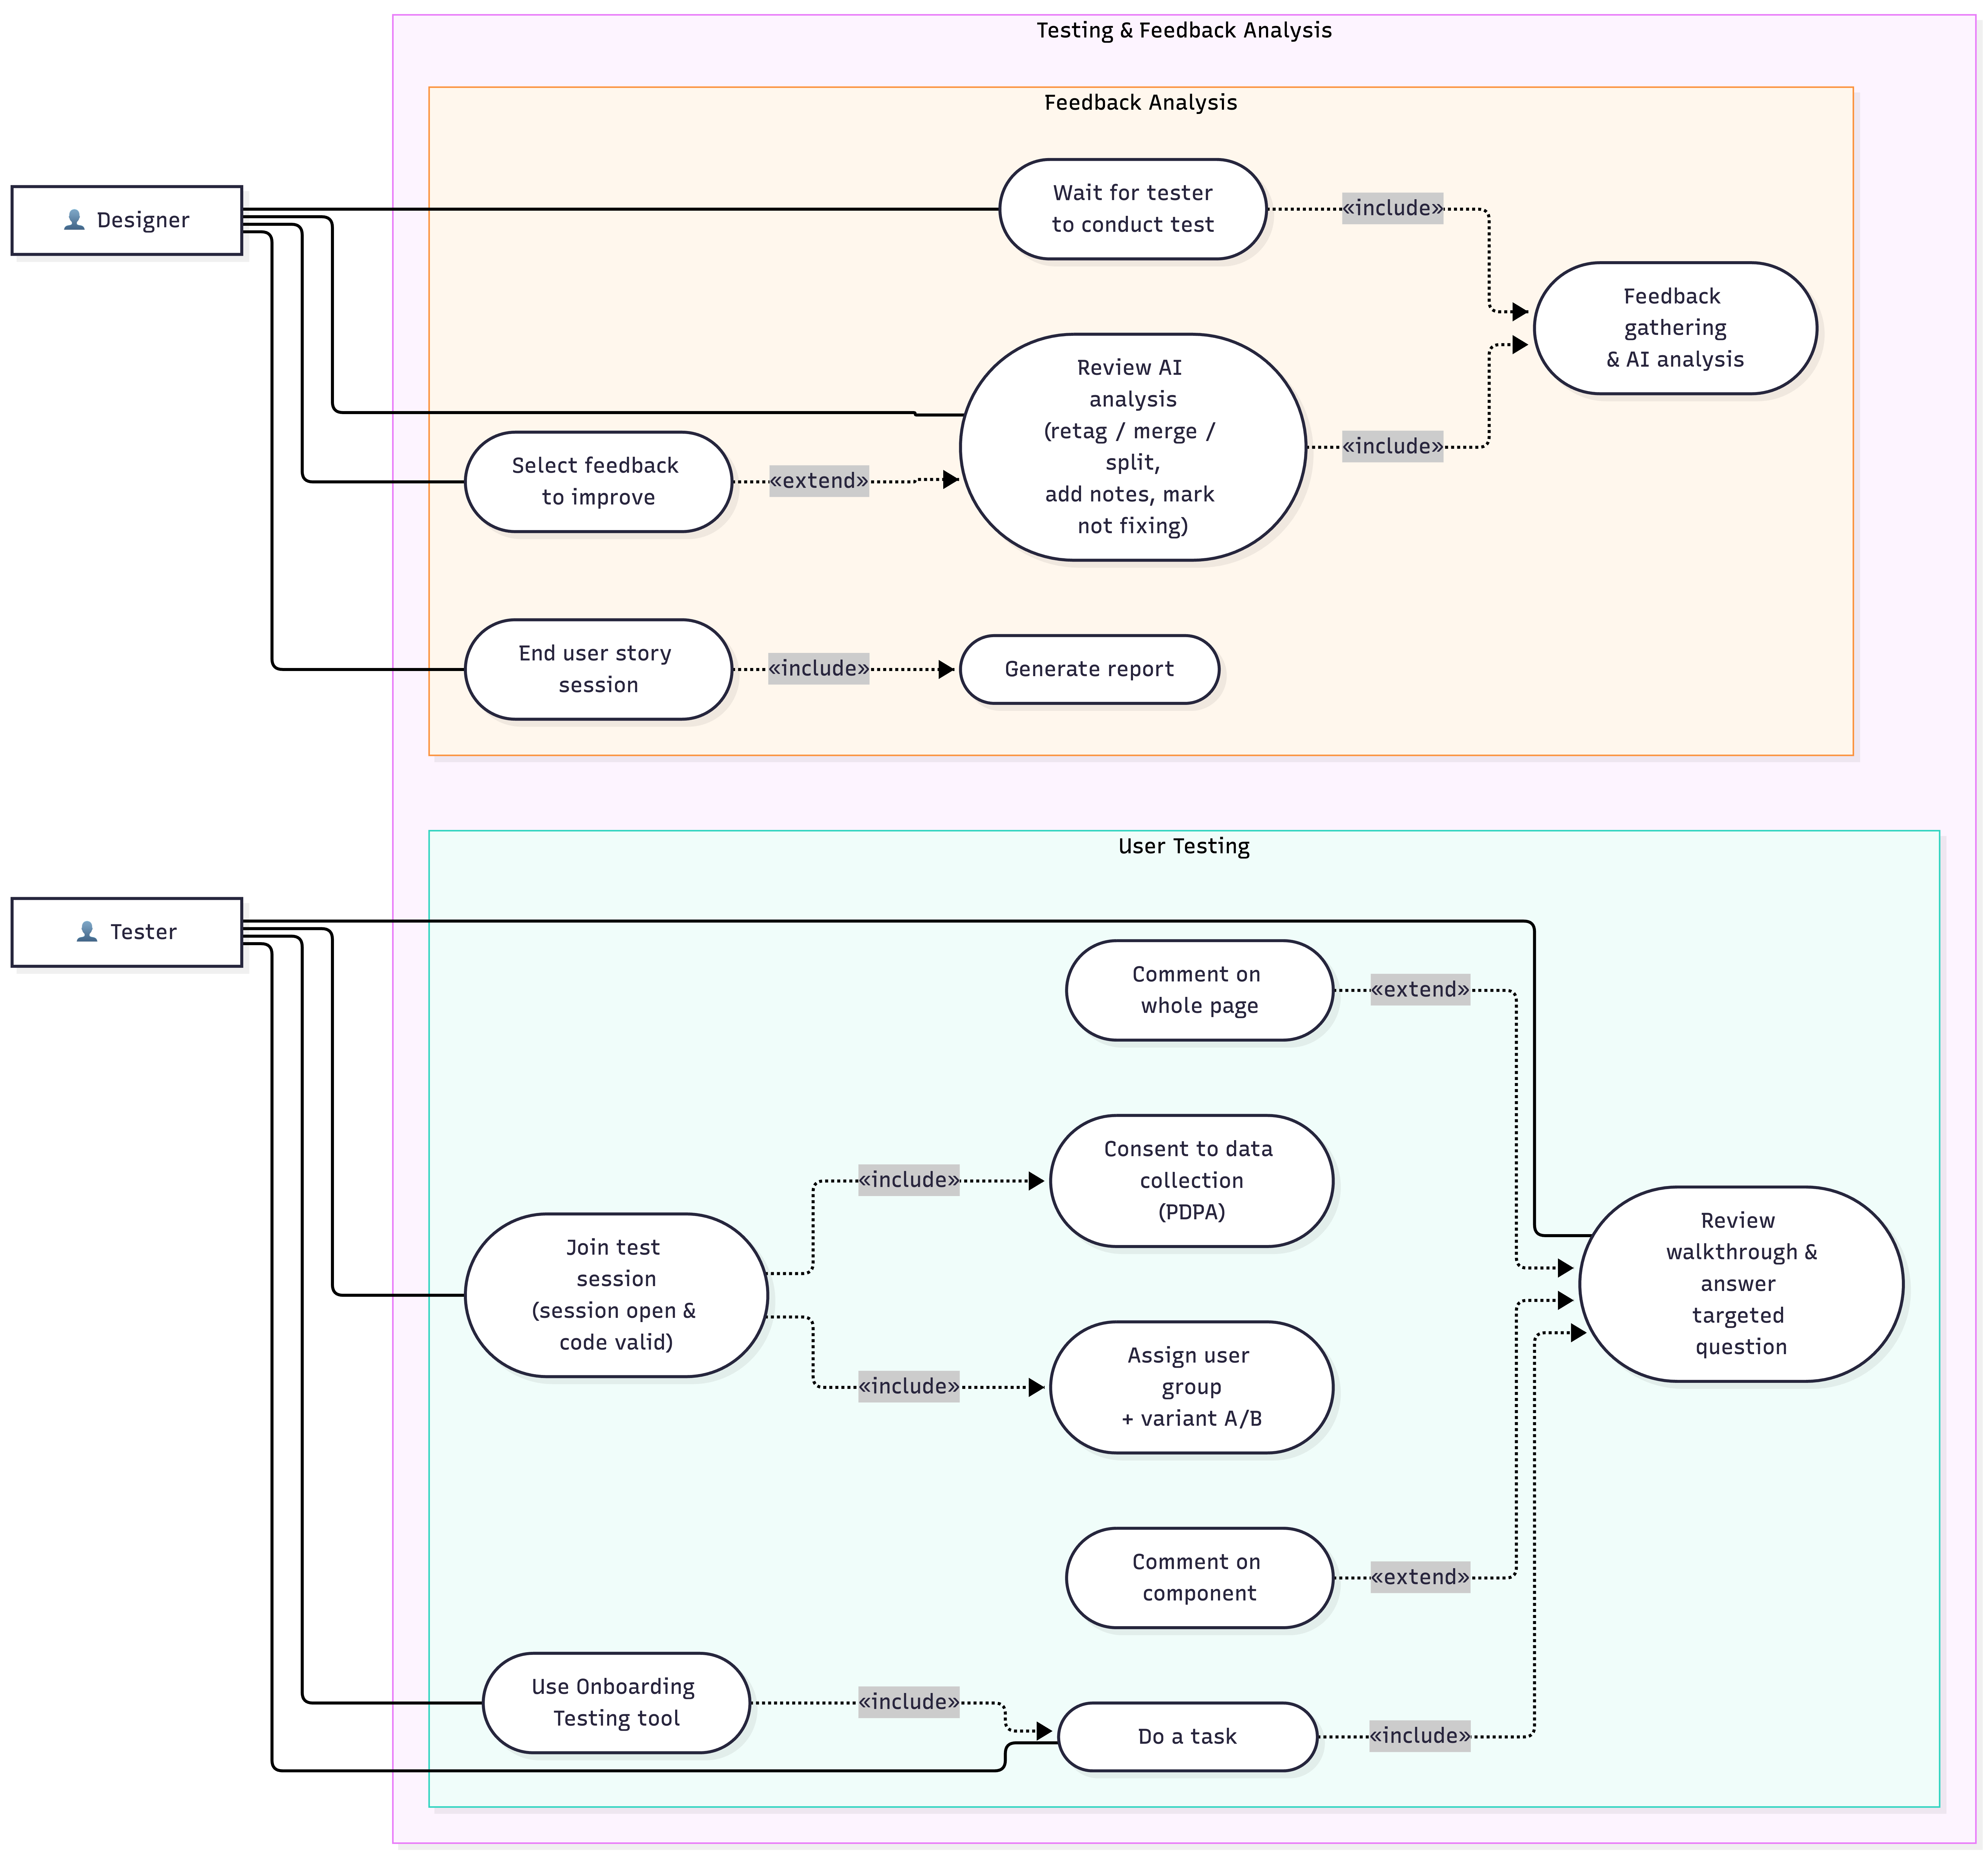
\includegraphics[
      width=0.6\textheight,
      height=\linewidth,
      keepaspectratio,
      origin=c
    ]{figures/ch3-methodology/UC-3.png}
    \caption{Use case diagram for Testing session and Feedback analysis}
    \label{fig:UC-3}
    \thaijustify{ภาพแสดง Use Case ของกระบวนการทดสอบและวิเคราะห์ Feedback โดย Tester เข้าร่วมการทดสอบ ทำภารกิจ และให้ความคิดเห็น ขณะที่ Designer รวบรวมและตรวจสอบผลการทดสอบ วิเคราะห์ Feedback ด้วย AI และเลือกประเด็นเพื่อนำไปปรับปรุงส่วนต่อประสานผู้ใช้}
  \end{figure}
  \subsubsection{Client, Developer, and Project Manager: Project view and Report}
  \begin{figure}[H]
    \centering
    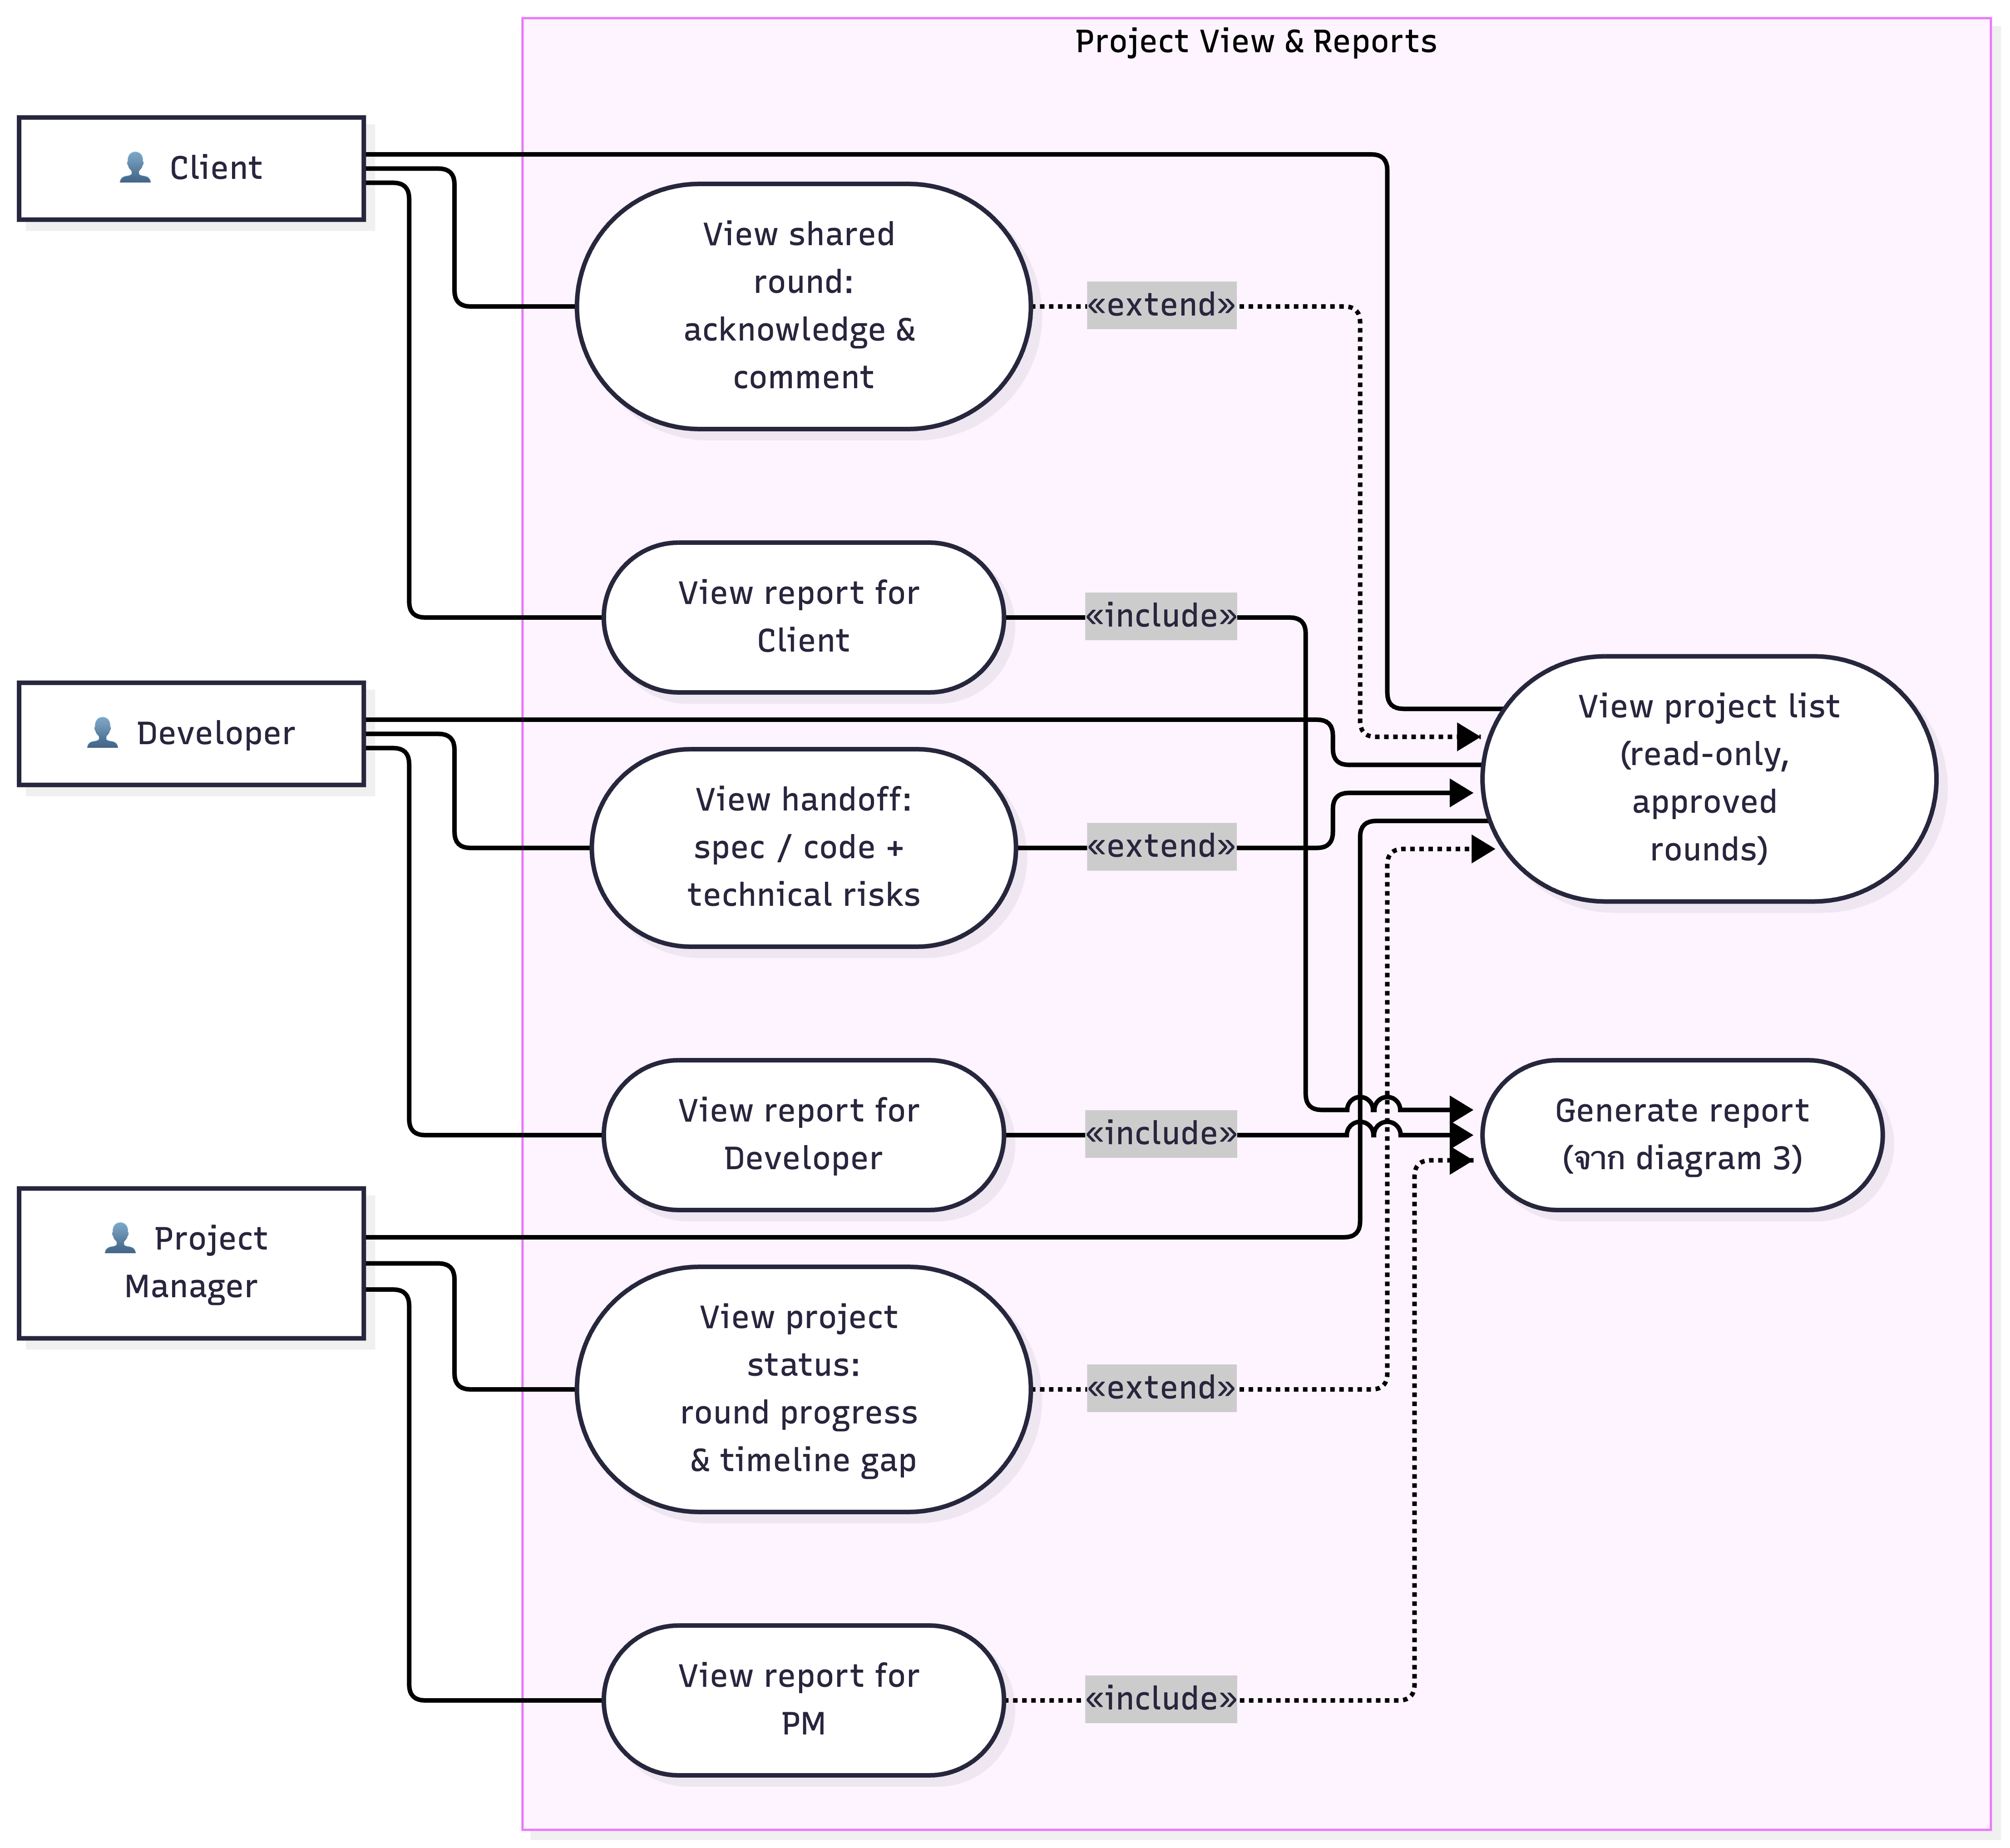
\includegraphics[
      width=0.6\textheight,
      height=\linewidth,
      keepaspectratio,
      origin=c
    ]{figures/ch3-methodology/UC-4.png}
    \caption{Use case diagram for Project view and Report}
    \label{fig:UC-4}
    \thaijustify{
      ภาพแสดง Use Case ของการดูโครงการและรายงาน โดย ผู้ใช้งาน, นักพัฒนา และ ผู้ดูแลโครงการ สามารถดูข้อมูลโครงการที่ได้รับอนุมัติและข้อมูลที่เกี่ยวข้องตามบทบาท รวมถึงดูรายงานที่สร้างจากผลการทดสอบและ Feedback
    }
  \end{figure}
\end{samepage}

\subsection{Sequence Diagram}
\thaijustify{
  \todo{Sequence diagram ของกระบวนการหลัก เช่น การสร้าง two-alternative UI และการทดสอบ}
}

\subsection{ER Diagram}\label{sec:er-diagram}
\thaijustify{
  ฐานข้อมูลของแพลตฟอร์มใช้ PostgreSQL และกำหนดโครงสร้างผ่าน Prisma schema ประกอบด้วย 34 ตารางและ 25 ชนิดข้อมูลแบบ enum เพื่อให้อ่านง่าย จึงแบ่ง ER diagram ออกเป็นสี่กลุ่มตามส่วนของระบบ (รูปที่~\ref{fig:er-workspace-project} ถึง~\ref{fig:er-analysis-report}) ในแต่ละตารางแสดง primary key (PK), foreign key (FK) และคอลัมน์หลักบางส่วน ส่วนตารางสีเทาเป็นตารางจากกลุ่มอื่นที่แสดงไว้เพื่อให้เห็นความสัมพันธ์
}
\thaijustify{
  \textbf{ผู้ใช้ workspace และโปรเจกต์ (รูปที่~\ref{fig:er-workspace-project}):} ผู้ใช้ (User) เข้าสู่ระบบผ่านบัญชีภายนอก (Account) และได้รับ refresh token ที่เก็บเป็นค่า hash แยกตามกลุ่มของการเข้าสู่ระบบ (familyId) ผู้ใช้สร้างหรือได้รับเชิญเข้า workspace โดยมีบทบาท ADMIN หรือ MEMBER (WorkspaceMember) ภายใน workspace มีหลายโปรเจกต์ (Project) และสมาชิกแต่ละคนมีบทบาทในโปรเจกต์ (ProjectMember) ได้แก่ Designer, Project Manager, Client และ Developer แต่ละโปรเจกต์มีความต้องการทางการออกแบบ (DesignIntent) หนึ่งชุด มี persona ได้หลายรายการ (UserPersona) และมีบันทึกกิจกรรม (AuditLog) สำหรับตรวจสอบย้อนหลัง
}
\thaijustify{
  \textbf{การออกแบบและการสร้าง UI ด้วย AI (รูปที่~\ref{fig:er-design-generation}):} โปรเจกต์มี user story (UserStory) ที่นักออกแบบเขียนเองหรือให้ AI ร่าง (StoryGeneration) แต่ละรอบการออกแบบ (DesignRound) อ้างอิง user story หนึ่งเรื่อง และอ้างอิงรอบก่อนหน้าได้ (parentRoundId) เมื่อสั่งสร้าง UI ระบบสร้างงาน (GenerationJob) ที่เก็บ prompt และจำนวน variant ไว้ ผลลัพธ์คือ UI variant (UIVariant) ซึ่งเก็บ HTML และผลการตรวจการเข้าถึง เมื่อนักออกแบบปรับแก้ variant ระบบสร้าง variant ใหม่ที่อ้างอิงฉบับเดิม (parentVariantId) จึงย้อนดูประวัติแต่ละเวอร์ชันได้
}
\thaijustify{
  \textbf{เซสชันการทดสอบ (รูปที่~\ref{fig:er-testing}):} เซสชันการทดสอบ (TestSession) ผูกกับรอบการออกแบบหนึ่งรอบ และเลือก variant ที่ใช้ทดสอบผ่านตาราง SessionVariant ผู้เข้าร่วมทดสอบ (SessionParticipant) ได้รับลิงก์เชิญที่เก็บเป็นค่า hash และต้องให้ความยินยอมตาม PDPA ก่อนเริ่ม ซึ่งบันทึกไว้ใน ConsentRecord พร้อมเวอร์ชันของข้อความที่ยินยอม ระหว่างทำภารกิจ (TestTask) ระบบบันทึกการทำภารกิจแต่ละครั้ง (TaskRun) พฤติกรรมการใช้งาน (InteractionEvent) และข้อเสนอแนะ (Feedback) ซึ่งระบุได้ว่าเป็นความเห็นต่อ component หรือต่อทั้งหน้าจอ
}
\thaijustify{
  \textbf{การวิเคราะห์ข้อเสนอแนะและรายงาน (รูปที่~\ref{fig:er-analysis-report}):} ผลการวิเคราะห์ข้อเสนอแนะด้วย AI เก็บใน FeedbackAnalysis และแยกเป็นประเด็น (FeedbackTheme) ที่เชื่อมกับข้อเสนอแนะต้นทางผ่าน ThemeFeedback นักออกแบบรวม แยก หรือตัดสินใจไม่แก้ไขประเด็นได้ ทุกการตัดสินใจถูกบันทึกใน DesignDecision และประเด็นที่เลือกไปปรับปรุงเชื่อมกับรอบการออกแบบถัดไปผ่าน RoundFeedbackLink ทำให้สืบย้อนได้ว่าการเปลี่ยนแปลงแต่ละครั้งมาจากข้อเสนอแนะใด ผู้มีส่วนได้ส่วนเสียแสดงความเห็นและรับทราบรอบที่อนุมัติแล้วได้ (RoundComment, RoundAcknowledgement) และระบบสร้างรายงาน (Report) แยกตามบทบาท
}

\begin{figure}[p]
  \centering
  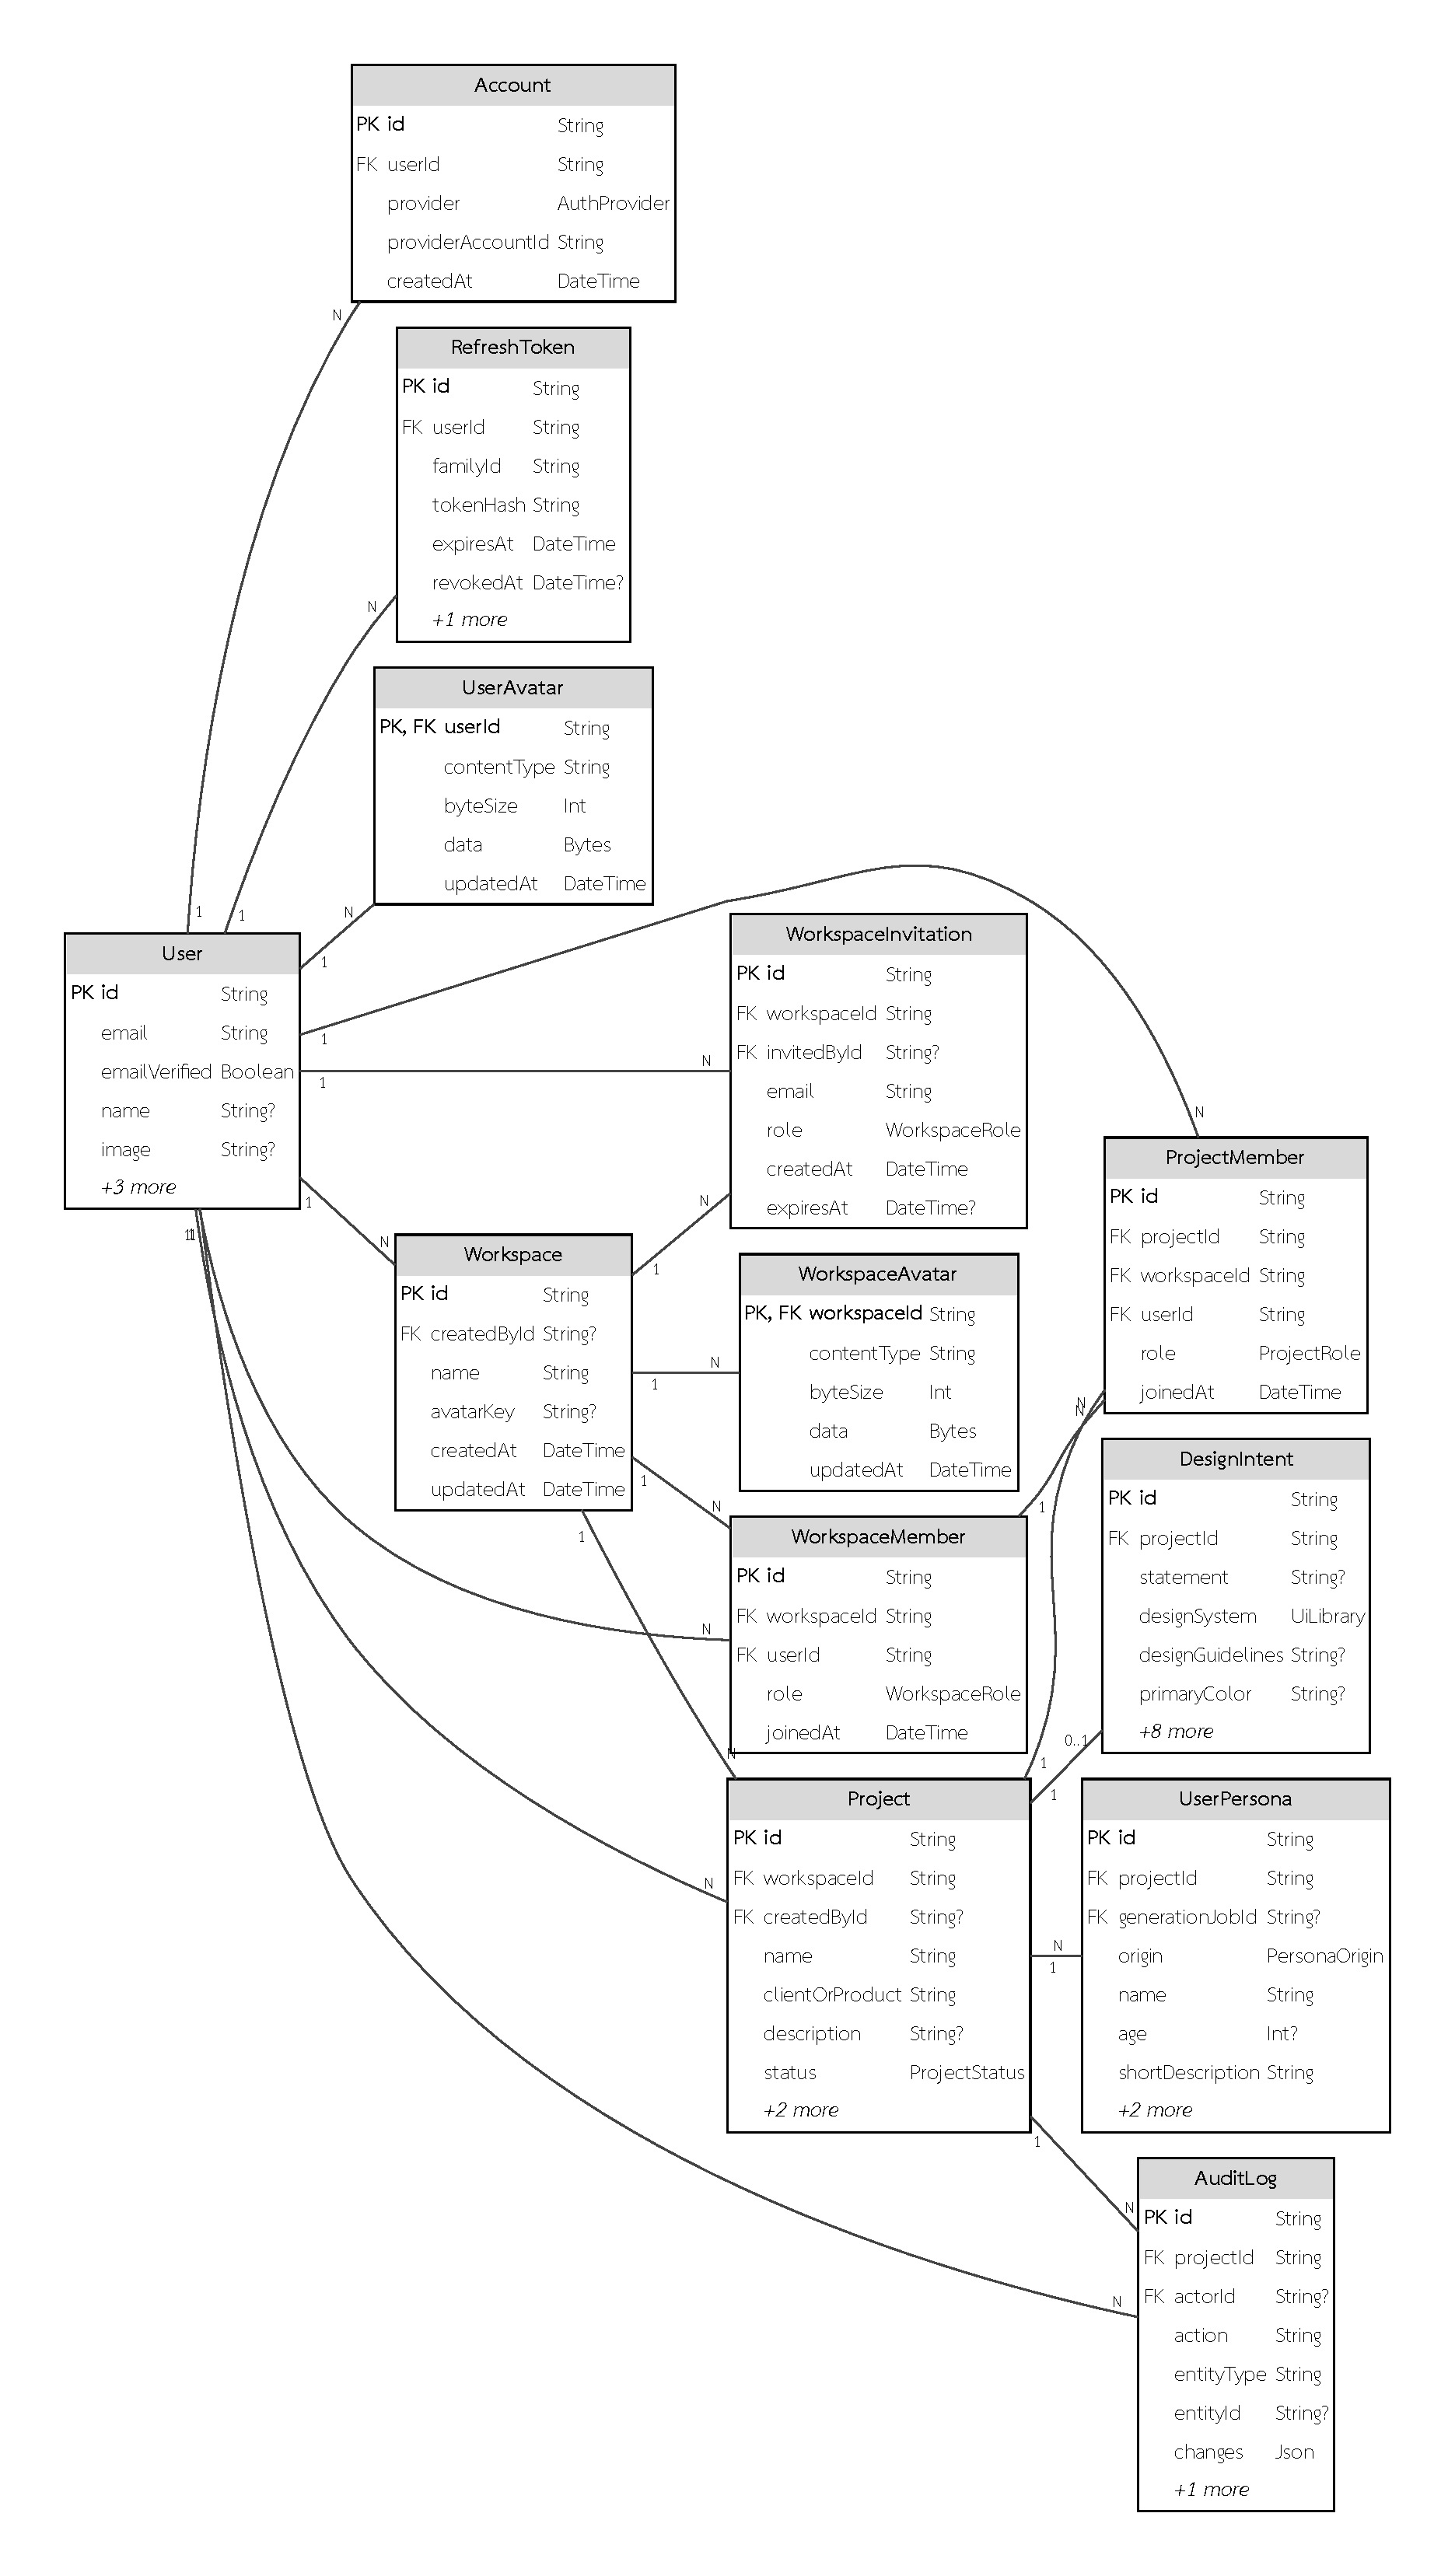
\includegraphics[width=\linewidth,height=0.88\textheight,keepaspectratio]{figures/ch3-methodology/er-workspace-project.pdf}
  \caption{ER diagram ส่วนผู้ใช้ workspace และโปรเจกต์}
  \label{fig:er-workspace-project}
\end{figure}
\begin{figure}[p]
  \centering
  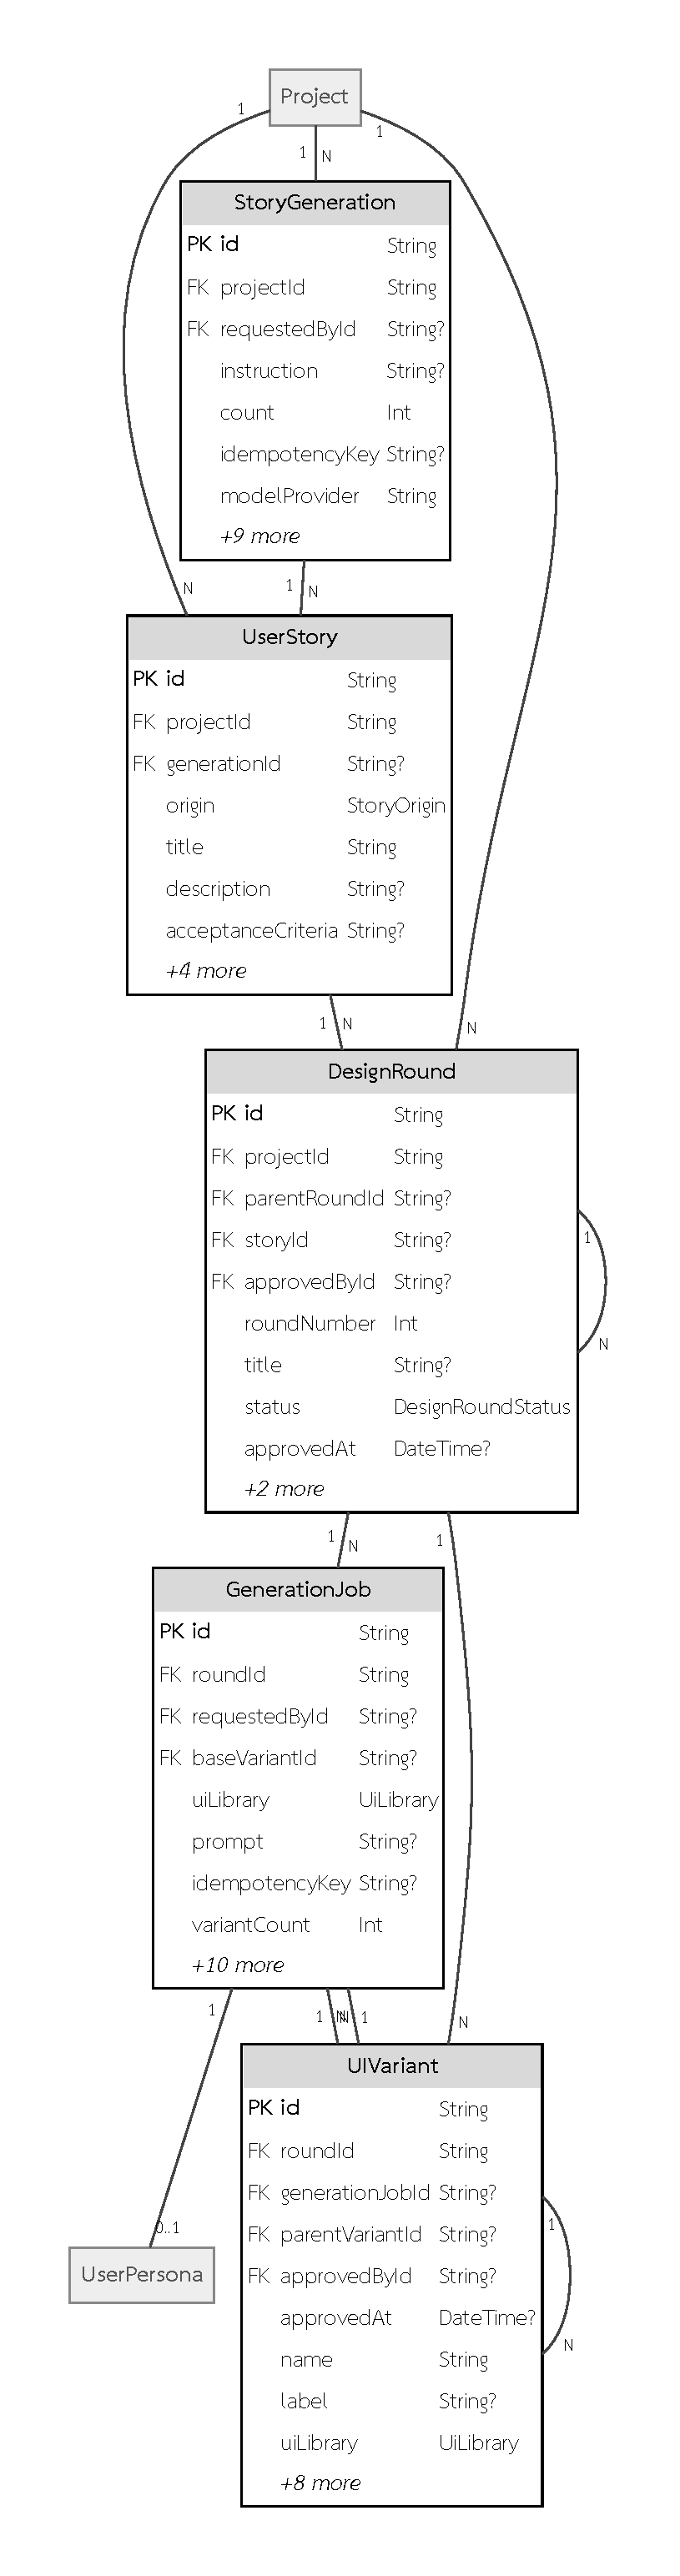
\includegraphics[width=\linewidth,height=0.88\textheight,keepaspectratio]{figures/ch3-methodology/er-design-generation.pdf}
  \caption{ER diagram ส่วนการออกแบบและการสร้าง UI ด้วย AI}
  \label{fig:er-design-generation}
\end{figure}
\begin{figure}[p]
  \centering
  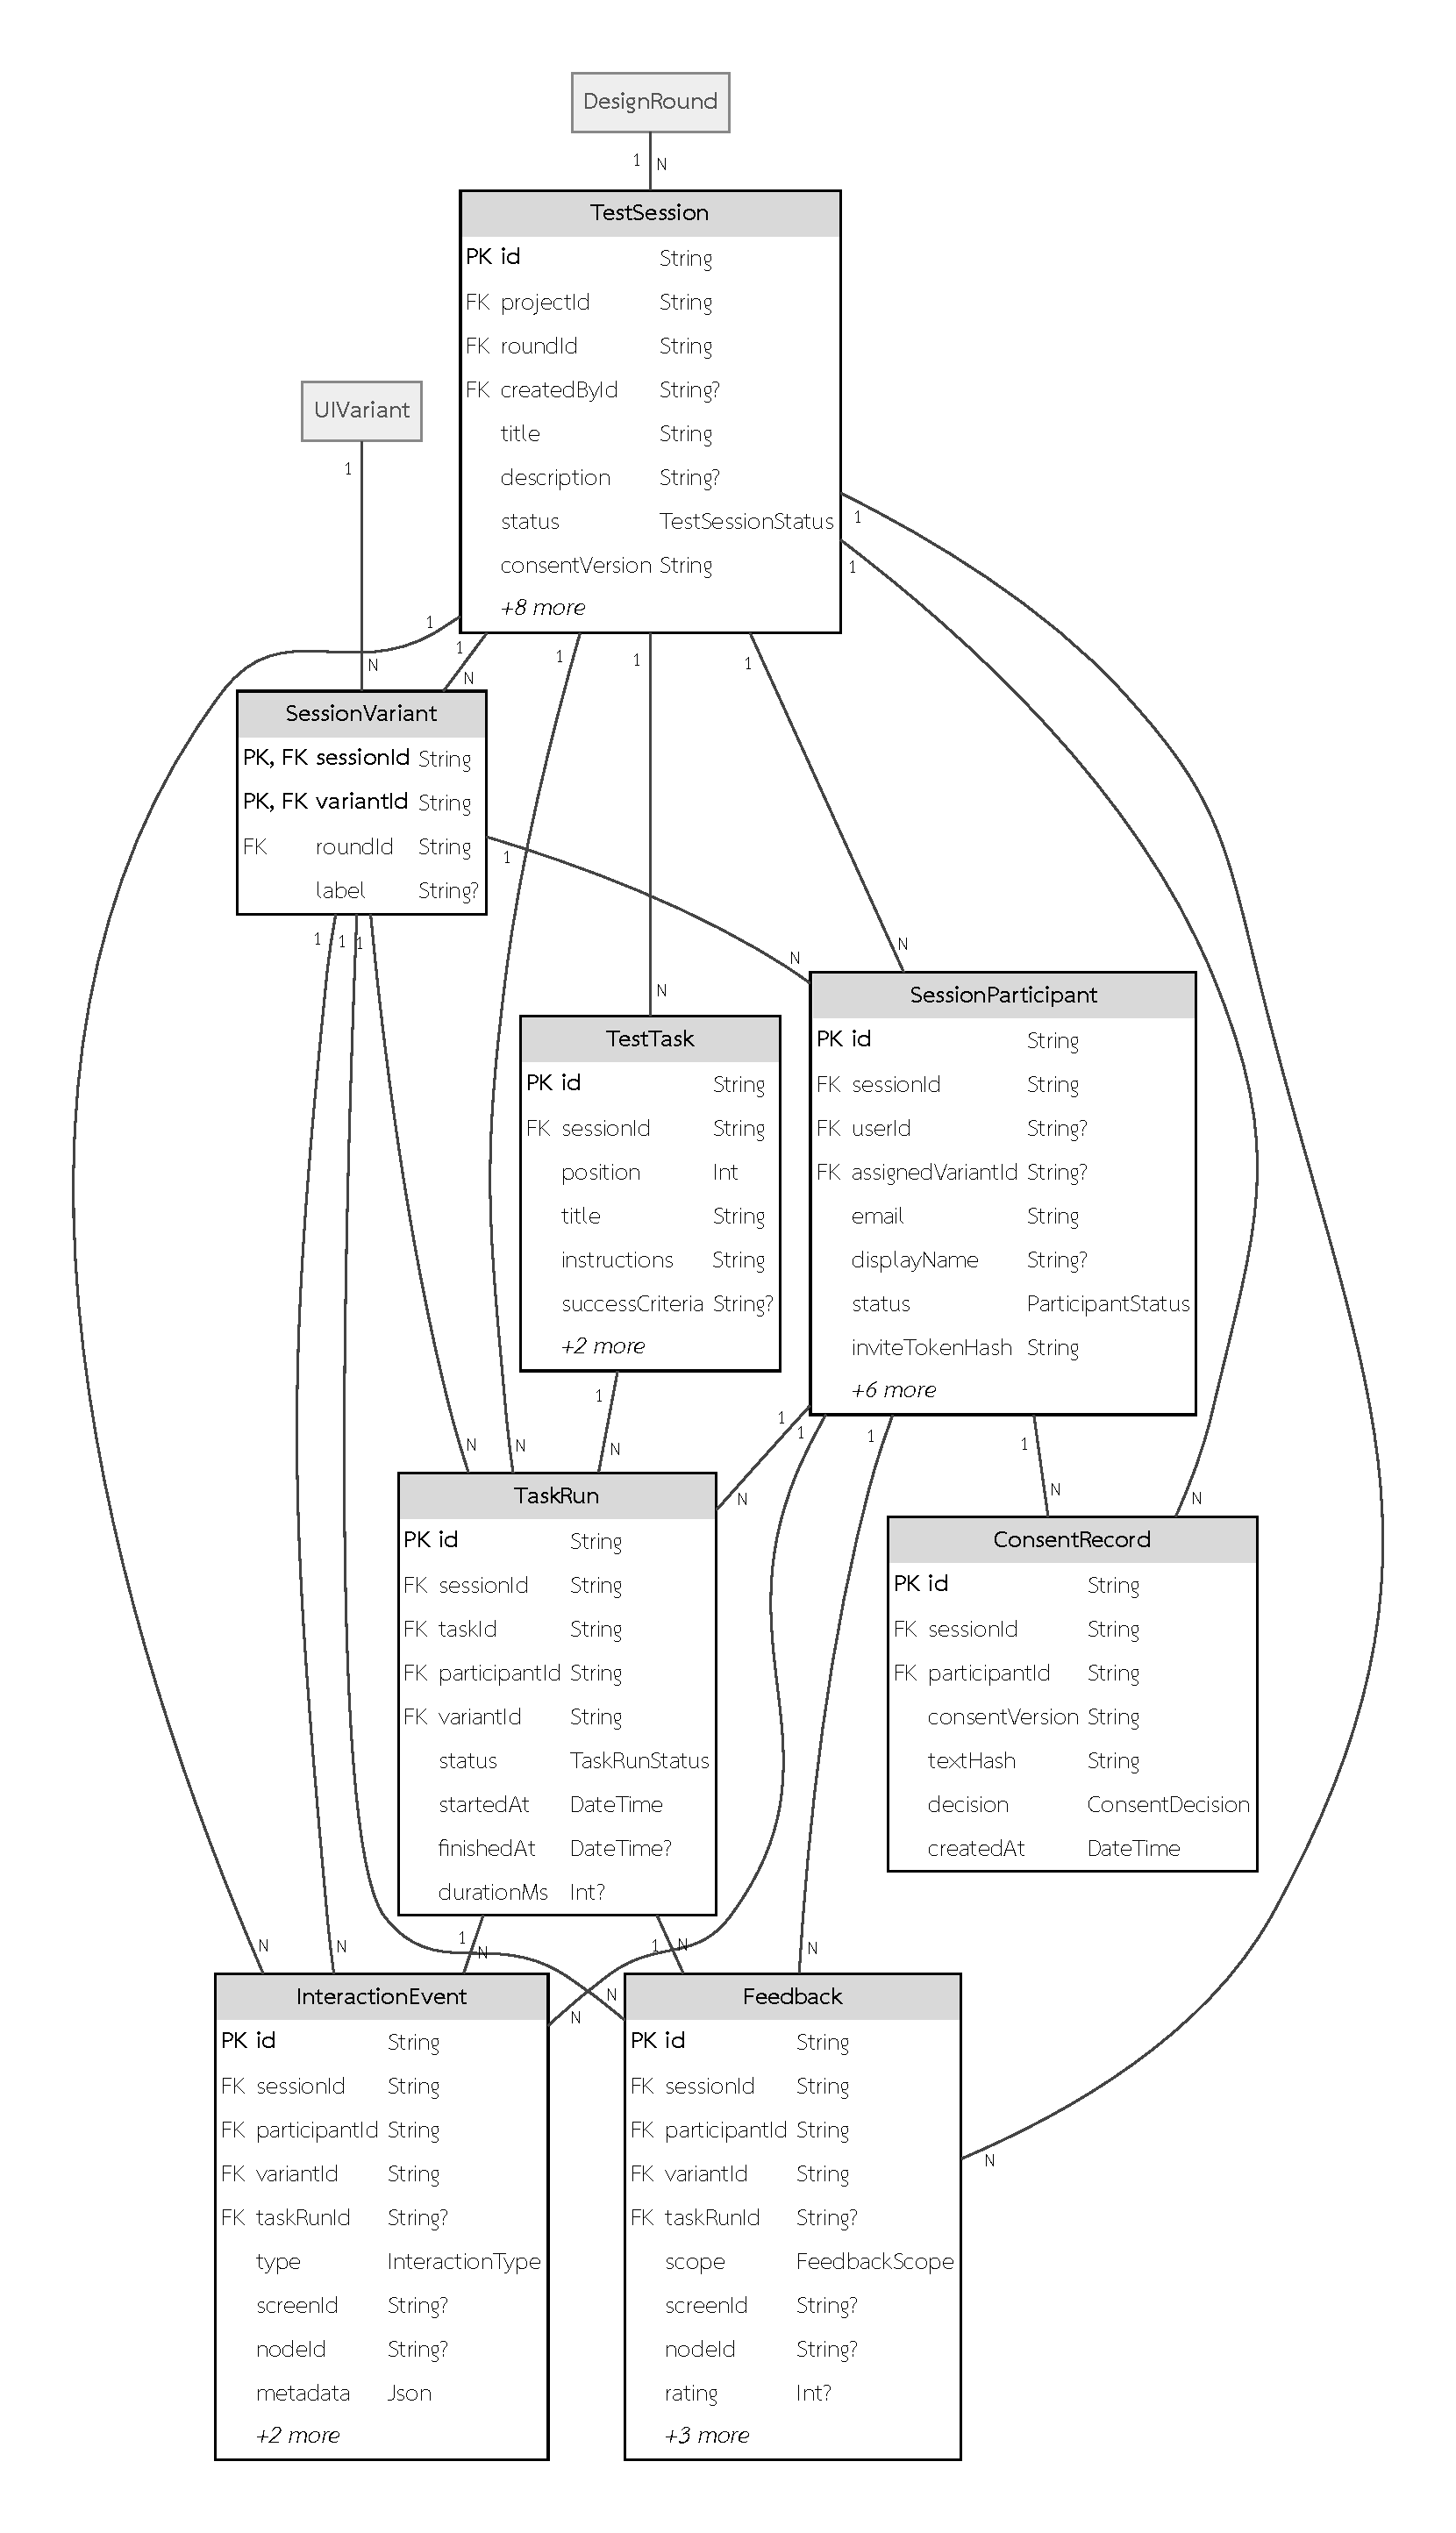
\includegraphics[width=\linewidth,height=0.88\textheight,keepaspectratio]{figures/ch3-methodology/er-testing.pdf}
  \caption{ER diagram ส่วนเซสชันการทดสอบ}
  \label{fig:er-testing}
\end{figure}
\begin{figure}[p]
  \centering
  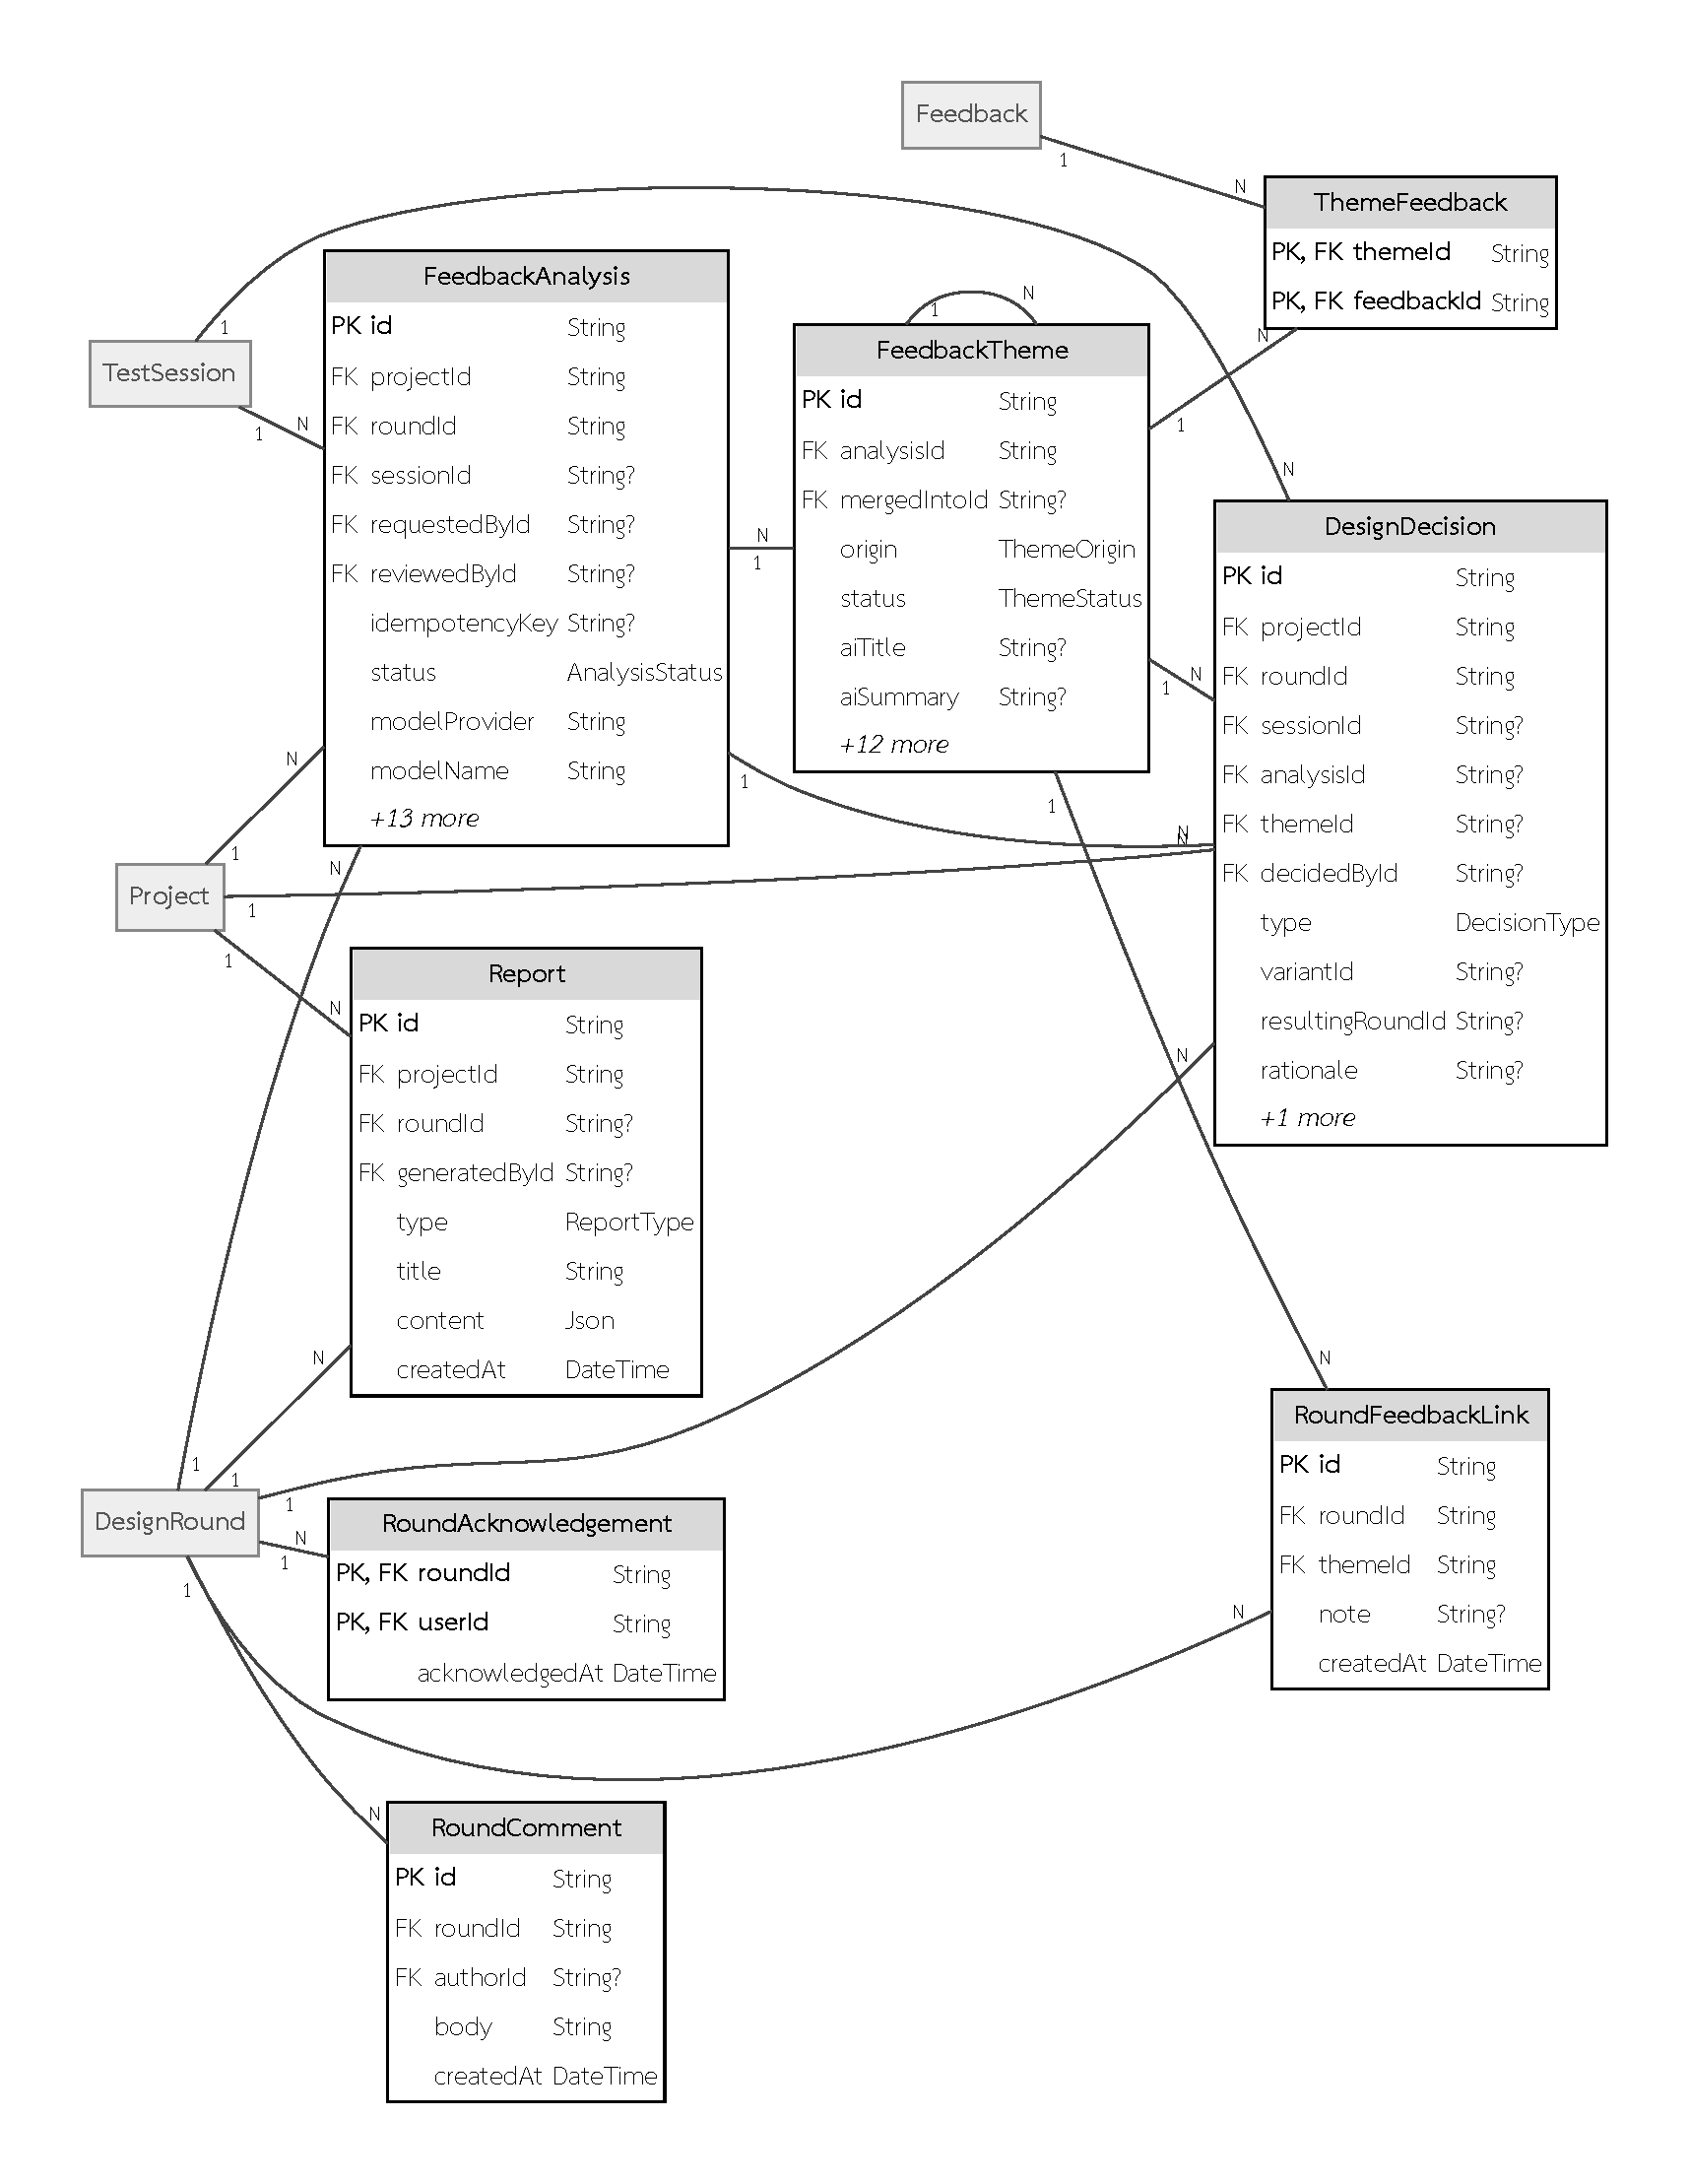
\includegraphics[width=\linewidth,height=0.88\textheight,keepaspectratio]{figures/ch3-methodology/er-analysis-report.pdf}
  \caption{ER diagram ส่วนการวิเคราะห์ข้อเสนอแนะและรายงาน}
  \label{fig:er-analysis-report}
\end{figure}

\subsection{User Flow และแผนผังเว็บไซต์ (Site Map)}
\thaijustify{
  \todo{User flow และ sitemap ให้ตรงกับ hi-fi v2}
}

% !TeX root = ../../progress-sem1.tex
% 3.x สถาปัตยกรรมโดยภาพรวมของระบบ
\section{สถาปัตยกรรมโดยภาพรวมของระบบ}
\begin{figure}[H]
  \centering
  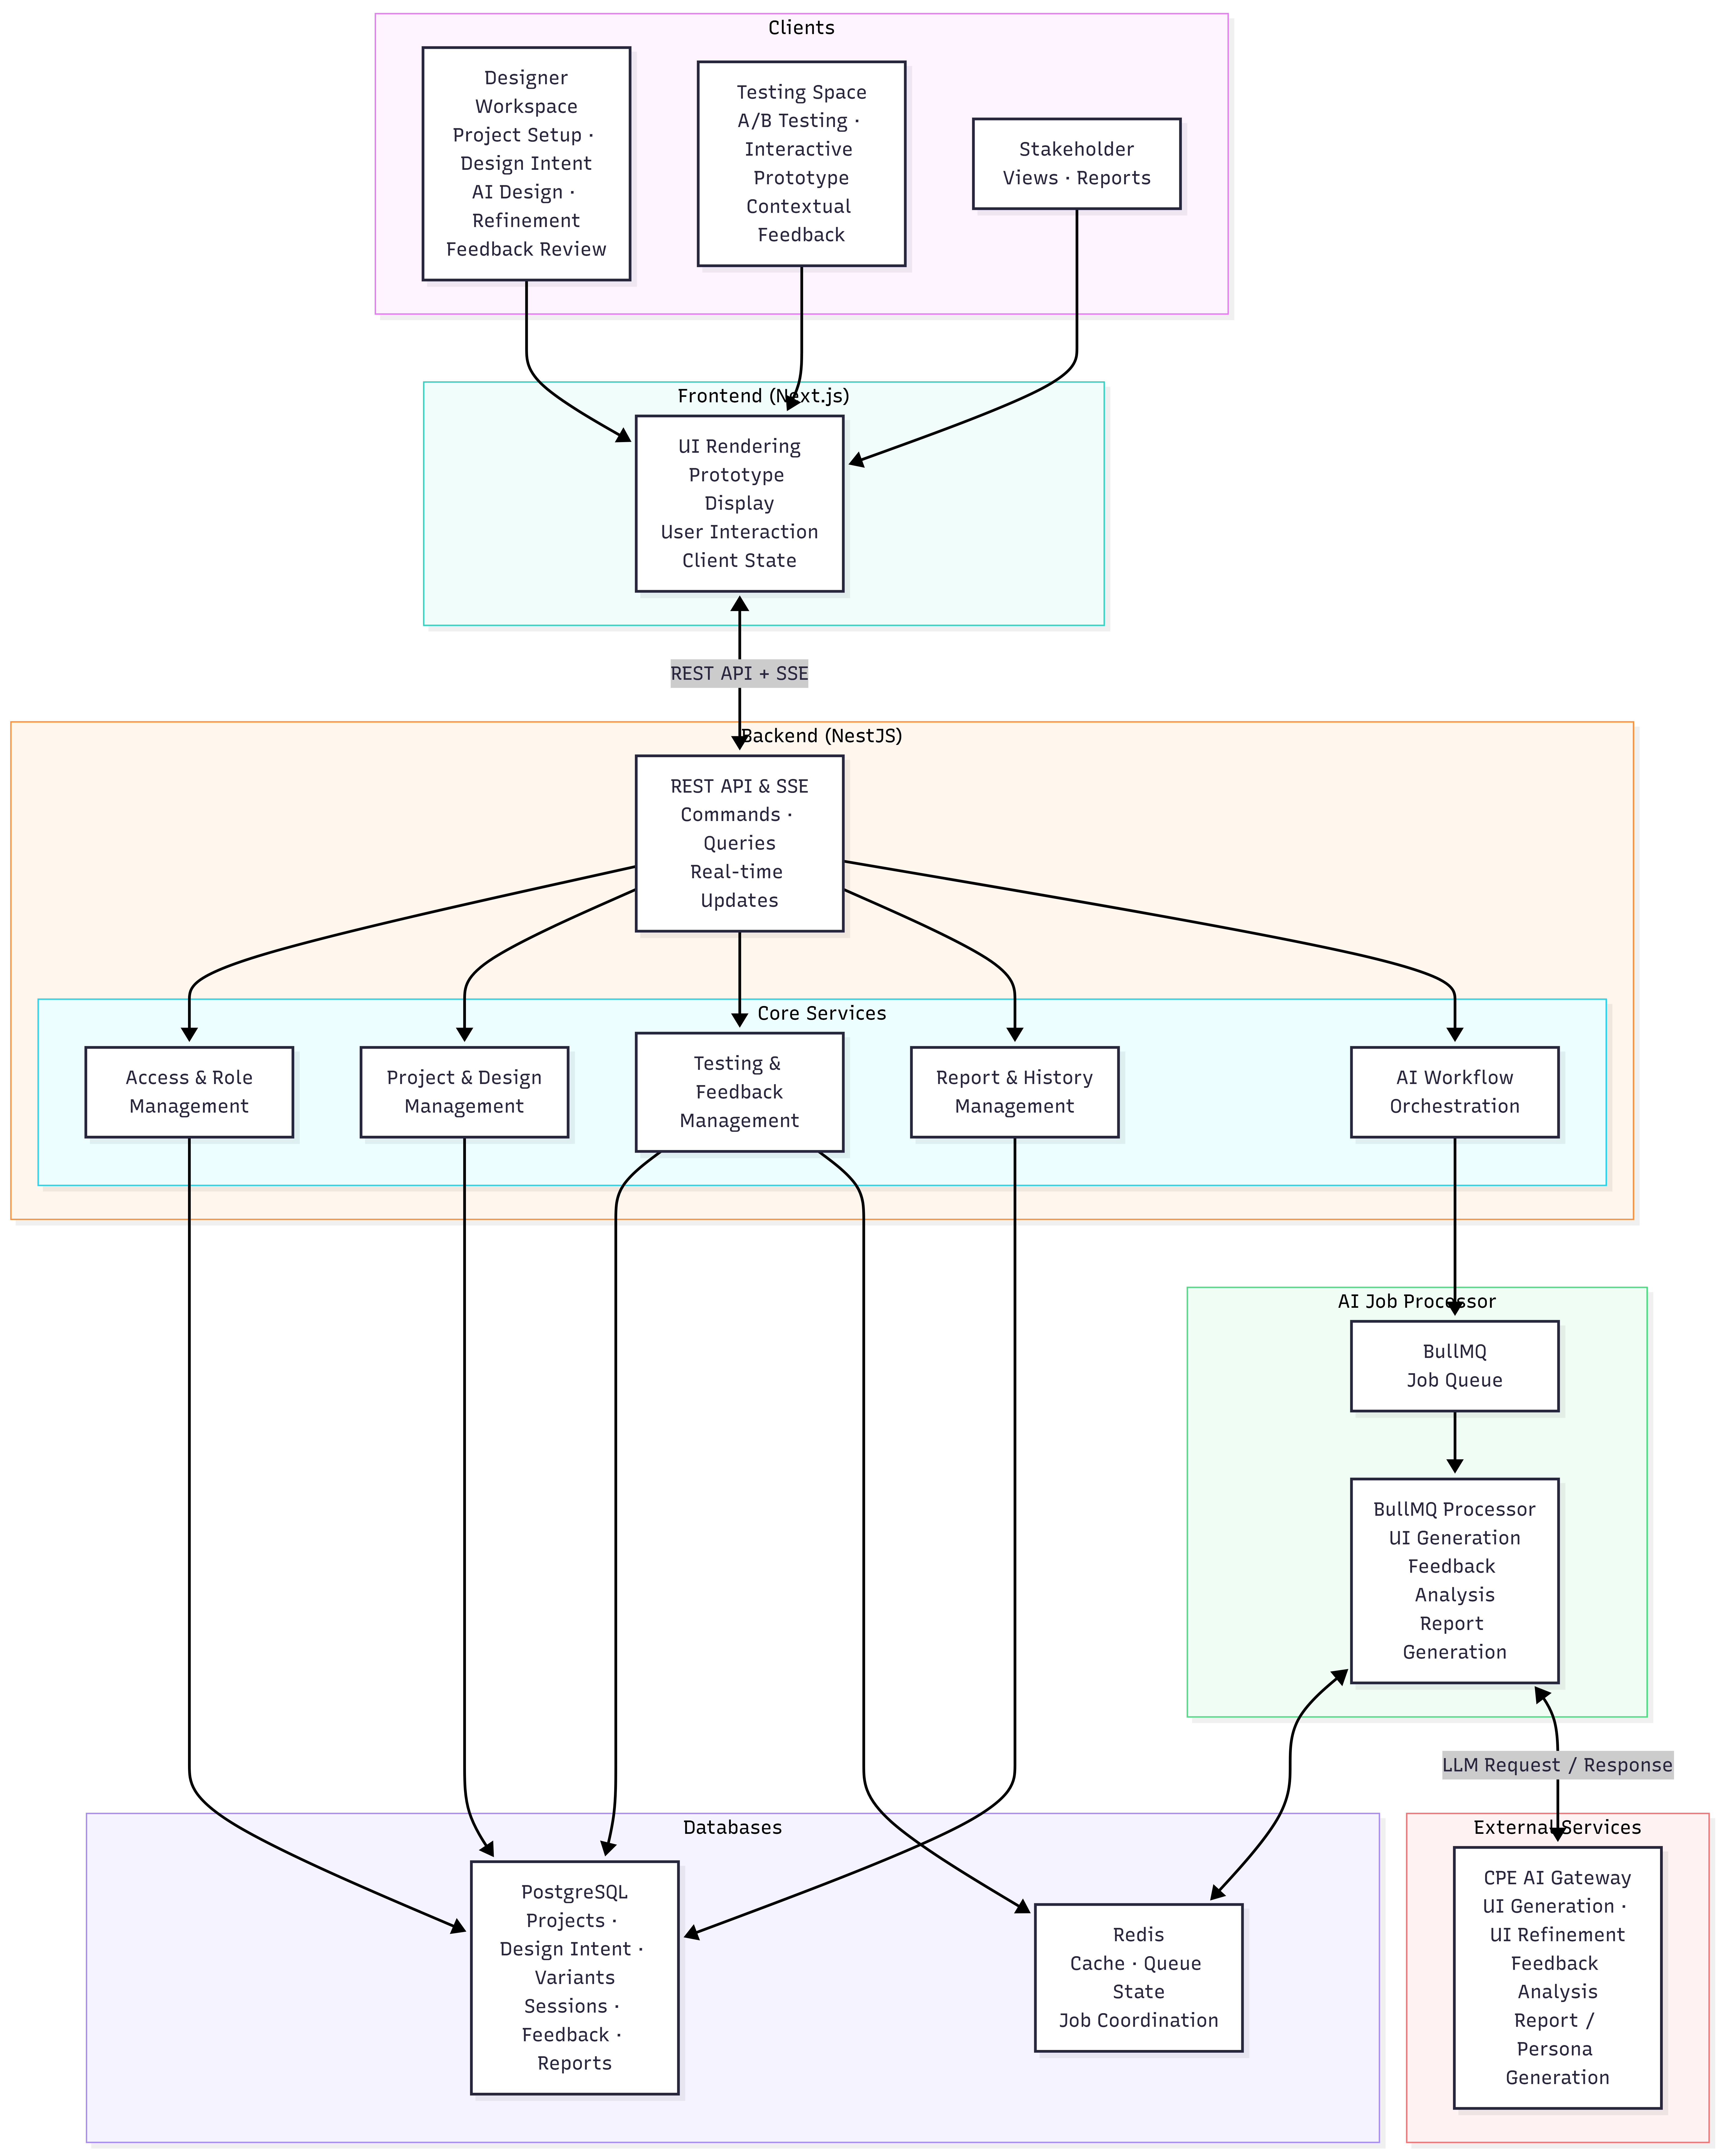
\includegraphics[
    width=0.8\linewidth,
    height=\textheight,
    keepaspectratio
  ]{figures/ch3-methodology/sys-arch3.png}
  \caption{System architecture}
  \label{fig:tech-stack-system-architecture}
  \thaijustify{ภาพแสดงสถาปัตยกรรมระบบโดยแบ่งออกเป็น Client, Frontend, Backend, AI Job Processor, Database และ External Services โดย Frontend พัฒนาด้วย Next.js และสื่อสารกับ Backend ผ่าน REST API และ SSE (Server-Sent Events) ซึ่งช่วยให้ Server สามารถส่งข้อมูลและการอัปเดตแบบ Real-time ไปยัง Client ได้โดยไม่ต้องส่ง Request ใหม่ ขณะที่ Backend ซึ่งพัฒนาด้วย NestJS ทำหน้าที่จัดการสิทธิ์ ข้อมูลโครงการ การทดสอบ Feedback รายงาน และกระบวนการ AI โดยงานที่ต้องใช้เวลาประมวลผลจะถูกส่งผ่าน BullMQ ไปยัง AI Job Processor และเชื่อมต่อกับ CPE AI Gateway สำหรับการประมวลผลด้วย AI}
\end{figure}

% !TeX root = ../../progress-sem1.tex
% Section 3.4 (subsections): one subsection per layer of the system architecture,
% matching "สถาปัตยกรรมโดยภาพรวมของระบบ" in Progress_Sem1_THAI_Example1.pdf.
% Input from chapters/03-methodology.tex, after the architecture figure.

\subsection{Client Side (ส่วนผู้ใช้งาน)}
\thaijustify{
  ผู้ใช้ทุกบทบาทเข้าใช้งานผ่านเว็บเบราว์เซอร์ นักออกแบบ (Designer) ใช้หน้าจอหลักของแพลตฟอร์มตั้งแต่การสร้างโปรเจกต์จนถึงการปรับแก้ UI ผู้เข้าร่วมทดสอบ (Usability Tester) เข้าร่วมเซสชันผ่านลิงก์เชิญโดยไม่ต้องสมัครสมาชิก ส่วน Client, Developer และ Project Manager ใช้มุมมองสำหรับติดตามสถานะ รับมอบงาน และดูรายงาน
}

\subsection{Frontend Layer}
\thaijustify{
  Frontend พัฒนาด้วย Next.js แบบ App Router แบ่ง route ออกเป็นกลุ่ม \texttt{(auth)} สำหรับการเข้าสู่ระบบ \texttt{(dashboard)} สำหรับ workspace และโปรเจกต์ และ \texttt{(legal)} สำหรับนโยบายความเป็นส่วนตัวและข้อกำหนดการใช้งาน หน้าจอสื่อสารกับ backend ผ่าน REST API และรับความคืบหน้าของงาน AI ผ่าน SSE หน้าตัวอย่าง UI ที่ AI สร้างแสดงใน iframe ที่ไม่อนุญาตให้รันสคริปต์ เพื่อป้องกันโค้ดที่ไม่ปลอดภัยจากผลลัพธ์ของโมเดล
}

\subsection{Backend API Layer}
\thaijustify{
  Backend พัฒนาด้วย NestJS แบบ monolith แบ่งเป็น module ตามโดเมน ได้แก่ \texttt{auth}, \texttt{access}, \texttt{users}, \texttt{workspaces}, \texttt{projects}, \texttt{design}, \texttt{rounds}, \texttt{generation}, \texttt{ai}, \texttt{testing}, \texttt{iteration}, \texttt{stakeholders}, \texttt{audit} และ \texttt{health} ทุก request ผ่านการตรวจ token การตรวจสิทธิ์ตาม permission การจำกัดอัตราการเรียก (rate limit) และ security header ก่อนถึง module ปลายทาง
}

\subsection{AI Job Processor Layer}
\thaijustify{
  งานที่ใช้เวลานานถูกส่งเข้าคิวของ BullMQ บน Redis แทนการประมวลผลใน request โดยตรง โดยแบ่งเป็นสองคิว ได้แก่ คิว design-generation สำหรับการสร้าง UI variant และการสังเคราะห์ persona และคิว ai-task สำหรับการร่าง user story และการวิเคราะห์ข้อเสนอแนะ worker ดึงงานจากคิว เรียกโมเดลผ่าน CPE AI Gateway ซึ่งมี API แบบเดียวกับ OpenAI และส่งความคืบหน้ากลับไปยังหน้าจอผ่าน SSE ผู้ใช้จึงปิดหน้าจอแล้วกลับมาติดตามงานเดิมต่อได้ รายละเอียดอยู่ในหัวข้อ~\ref{sec:ai-pipeline}
}

\subsection{Data \& External Services Layer}
\thaijustify{
  PostgreSQL จัดเก็บข้อมูลทั้งหมดของระบบผ่าน Prisma (หัวข้อ~\ref{sec:er-diagram}) Redis ทำหน้าที่ทั้งคิวงานและ cache ของ response บริการภายนอกที่ใช้ ได้แก่ Google OAuth 2.0 สำหรับการเข้าสู่ระบบ และ CPE AI Gateway ของภาควิชาซึ่งเข้าถึงได้ผ่าน VPN ของมหาวิทยาลัยเท่านั้น
}


\subsection{เทคโนโลยีที่ใช้ในแต่ละส่วน}
\thaijustify{
  ซอร์สโค้ดทั้งหมดจัดเก็บใน repository เดียวแบบ monorepo จัดการด้วย Turborepo และ pnpm แบ่งเป็นสองแอปพลิเคชัน คือ frontend และ backend เทคโนโลยีที่ใช้ในแต่ละส่วนแสดงในตารางที่~\ref{tab:tech-stack}
}
\begin{table}[H]
  \centering
  \caption{เทคโนโลยีที่ใช้ในแต่ละส่วนของระบบ}
  \label{tab:tech-stack}
  \small
  \begin{tabularx}{\linewidth}{|>{\RaggedRight\arraybackslash}p{0.2\linewidth}|>{\RaggedRight\arraybackslash}p{0.3\linewidth}|>{\RaggedRight\arraybackslash}X|}
    \hline
    \textbf{ส่วนของระบบ} & \textbf{เทคโนโลยี} & \textbf{หน้าที่} \\ \hline
    Frontend & Next.js 16, React 19, TypeScript & หน้าจอของผู้ใช้ทุกบทบาท \\ \hline
    UI library & shadcn/ui (Radix UI), Tailwind CSS, Hugeicons & component และไอคอนตาม design system ของแพลตฟอร์ม \\ \hline
    Backend & NestJS 11, TypeScript & REST API, การยืนยันตัวตน, การควบคุมสิทธิ์ และงาน AI \\ \hline
    ฐานข้อมูล & PostgreSQL 17, Prisma 7 & จัดเก็บข้อมูลทั้งหมด และจัดการ migration ของ schema \\ \hline
    Cache และคิวงาน & Redis 7, BullMQ & cache ของ response และคิวงานที่ใช้เวลานาน เช่น การสร้าง UI \\ \hline
    การสื่อสารแบบ real-time & Server-Sent Events (SSE) & ส่งความคืบหน้าและความคิดของโมเดลระหว่างประมวลผลไปยังหน้าจอ \\ \hline
    การยืนยันตัวตน & Passport (Google OAuth 2.0), JWT & เข้าสู่ระบบและออก access token กับ refresh token \\ \hline
    บริการ AI & CPE AI Gateway (API แบบเดียวกับ OpenAI) & muse-glimmer-30b สร้าง UI และ qwen3.8-27b วิเคราะห์ข้อเสนอแนะ ร่าง user story, prompt และ persona \\ \hline
    เอกสาร API & Swagger (OpenAPI) & เอกสารและเครื่องมือทดลองเรียก API \\ \hline
    การทดสอบ & Jest & unit test และ end-to-end test ของ backend \\ \hline
    CI & GitHub Actions & ตรวจชื่อ pull request, lint และ build ทุก pull request \\ \hline
  \end{tabularx}
\end{table}

% !TeX root = ../../progress-sem1.tex
% Section 3.5: UI prototype, split like the example
% (การออกแบบ UI / prototype ของผู้ใช้แต่ละกลุ่ม).
% Input from chapters/03-methodology.tex.

\section{การออกแบบ User Interface Prototype}\label{sec:ui-prototype}
\thaijustify{
  ทีมออกแบบหน้าจอแบบ high-fidelity ด้วย Figma ก่อนพัฒนา โดยแบ่งตามกลุ่มผู้ใช้ของแพลตฟอร์ม
}

\subsection{การออกแบบ UI (User Interface)}
\thaijustify{
  หน้าจอของแพลตฟอร์มใช้ design system ที่สร้างบน shadcn/ui และ Tailwind CSS ไอคอนใช้ชุด Hugeicons ทั้งระบบ
  \todo{โทนสี ตัวอักษร ขนาด spacing และ component หลักใน Figma พร้อมภาพ style guide}
}

\subsection{User Interface Prototype ของ Designer}
\thaijustify{
  \todo{ภาพ prototype ของ Designer: dashboard, การสร้างโปรเจกต์และ design intent, user story, การตรวจ prompt, generation trace และหน้า refine}
}

\subsection{User Interface Prototype ของ Usability Tester}
\thaijustify{
  \todo{ภาพ prototype ของผู้เข้าร่วมทดสอบ: หน้าเข้าร่วมเซสชัน, การให้ความยินยอม (PDPA), การทำภารกิจ และแบบฟอร์มข้อเสนอแนะ}
}

\subsection{User Interface Prototype ของ Client, Developer และ Project Manager}
\thaijustify{
  \todo{ภาพ prototype ของมุมมองผู้มีส่วนได้ส่วนเสีย: สถานะโปรเจกต์, handoff และรายงาน}
}

% !TeX root = ../../progress-sem1.tex
% Section: AI pipeline development, matching "การพัฒนา AI pipeline" in the example.
% Input from chapters/03-methodology.tex, before "การพัฒนาระบบ".

\section{การพัฒนา AI pipeline}\label{sec:ai-pipeline}
\thaijustify{
  AI ในแพลตฟอร์มทำงานสี่ส่วน ได้แก่ การร่าง user story การร่าง structured prompt การสร้าง UI variant และการวิเคราะห์ข้อเสนอแนะของผู้เข้าร่วมทดสอบ ในภาคการศึกษาที่ 1 ทีมพัฒนาสามส่วนแรกจนใช้งานผ่านหน้าจอได้ และพัฒนาส่วนการวิเคราะห์ข้อเสนอแนะไว้ที่ backend
}

\subsection{วิเคราะห์ความต้องการของระบบที่ใช้ AI}
\thaijustify{
  ผลลัพธ์ของ AI ต้องนำไปใช้ต่อในระบบได้ทันที จึงกำหนดให้โมเดลตอบเป็น JSON ตาม schema (structured output) และ UI ที่สร้างต้องเป็น HTML ที่ใช้ component ของ UI kit ที่นักออกแบบเลือก ใช้สีแบรนด์ตาม design intent และผ่านมาตรฐานการเข้าถึงที่กำหนด นอกจากนี้งานแต่ละชิ้นใช้เวลาหลายนาที ระบบจึงต้องแสดงความคืบหน้าแบบ real-time และให้ผู้ใช้ยกเลิกงานได้
}

\subsection{การเลือกโมเดลและบริการ AI}
\thaijustify{
  ระบบเรียกโมเดลผ่าน CPE AI Gateway ของภาควิชา ซึ่งให้บริการ API แบบเดียวกับ OpenAI จึงเปลี่ยนโมเดลได้ด้วยการตั้งค่า โดยไม่ต้องแก้โค้ด โมเดลที่ใช้ ได้แก่ muse-glimmer-30b สำหรับสร้าง UI และ qwen3.8-27b สำหรับงานที่ต้องการ structured output เช่น การร่าง prompt, user story, persona และการวิเคราะห์ข้อเสนอแนะ ระบบเปิดขั้นการคิด (reasoning) ของโมเดลไว้เป็นค่าเริ่มต้น เพื่อแสดงความคิดของโมเดลใน generation trace
  ทีมเลือกใช้โมเดลทั้งสองเนื่องจากเป็นโมเดลที่ภาควิชาเปิดให้ใช้ได้โดยไม่มีค่าใช้จ่าย จึงเหมาะกับช่วงพัฒนาที่ต้องเรียกโมเดลซ้ำหลายครั้ง
}

\subsection{การร่าง Structured Prompt}
\thaijustify{
  เมื่อนักออกแบบเลือก user story ระบบรวม design intent, persona และ user story เป็น context แล้วให้โมเดลร่าง structured prompt งานนี้รันเป็น background job บน BullMQ หน้าจอจึงกลับมาเชื่อมต่อกับงานเดิมผ่าน SSE ได้หากผู้ใช้ออกจากหน้าแล้วกลับมา ระบบแสดงจำนวน token ระหว่างร่าง และไม่บันทึกความคิดดิบของโมเดลลงฐานข้อมูล
}

\subsection{การสร้าง UI Variant พร้อมการตรวจและแก้ไขอัตโนมัติ}
\thaijustify{
  การสร้าง UI เป็นไปตามขั้นตอนในรูปที่~\ref{fig:generation-pipeline} ระบบสร้าง persona artifact จาก prompt ก่อน (ข้ามขั้นนี้ได้หากนักออกแบบเลือก persona ไว้แล้ว) จากนั้นสร้างหน้าจอแบบ high-fidelity เป็น HTML ทีละ variant ค่าเริ่มต้นคือสอง variant (A และ B) สำหรับ comparative usability testing HTML ที่ได้จะถูก sanitize และตรวจโครงสร้าง การใช้ component ของ UI kit สีแบรนด์ platform และการเข้าถึงตามมาตรฐานใน design intent หากไม่ผ่าน ระบบส่งปัญหาที่พบกลับให้โมเดลแก้ได้สูงสุดสองครั้ง และหากยังไม่ผ่านจะเริ่มสร้าง variant นั้นใหม่อีกหนึ่งครั้งโดยแจ้งโมเดลว่าครั้งก่อนผิดพลาดตรงไหน
}
\begin{figure}[H]
  \centering
  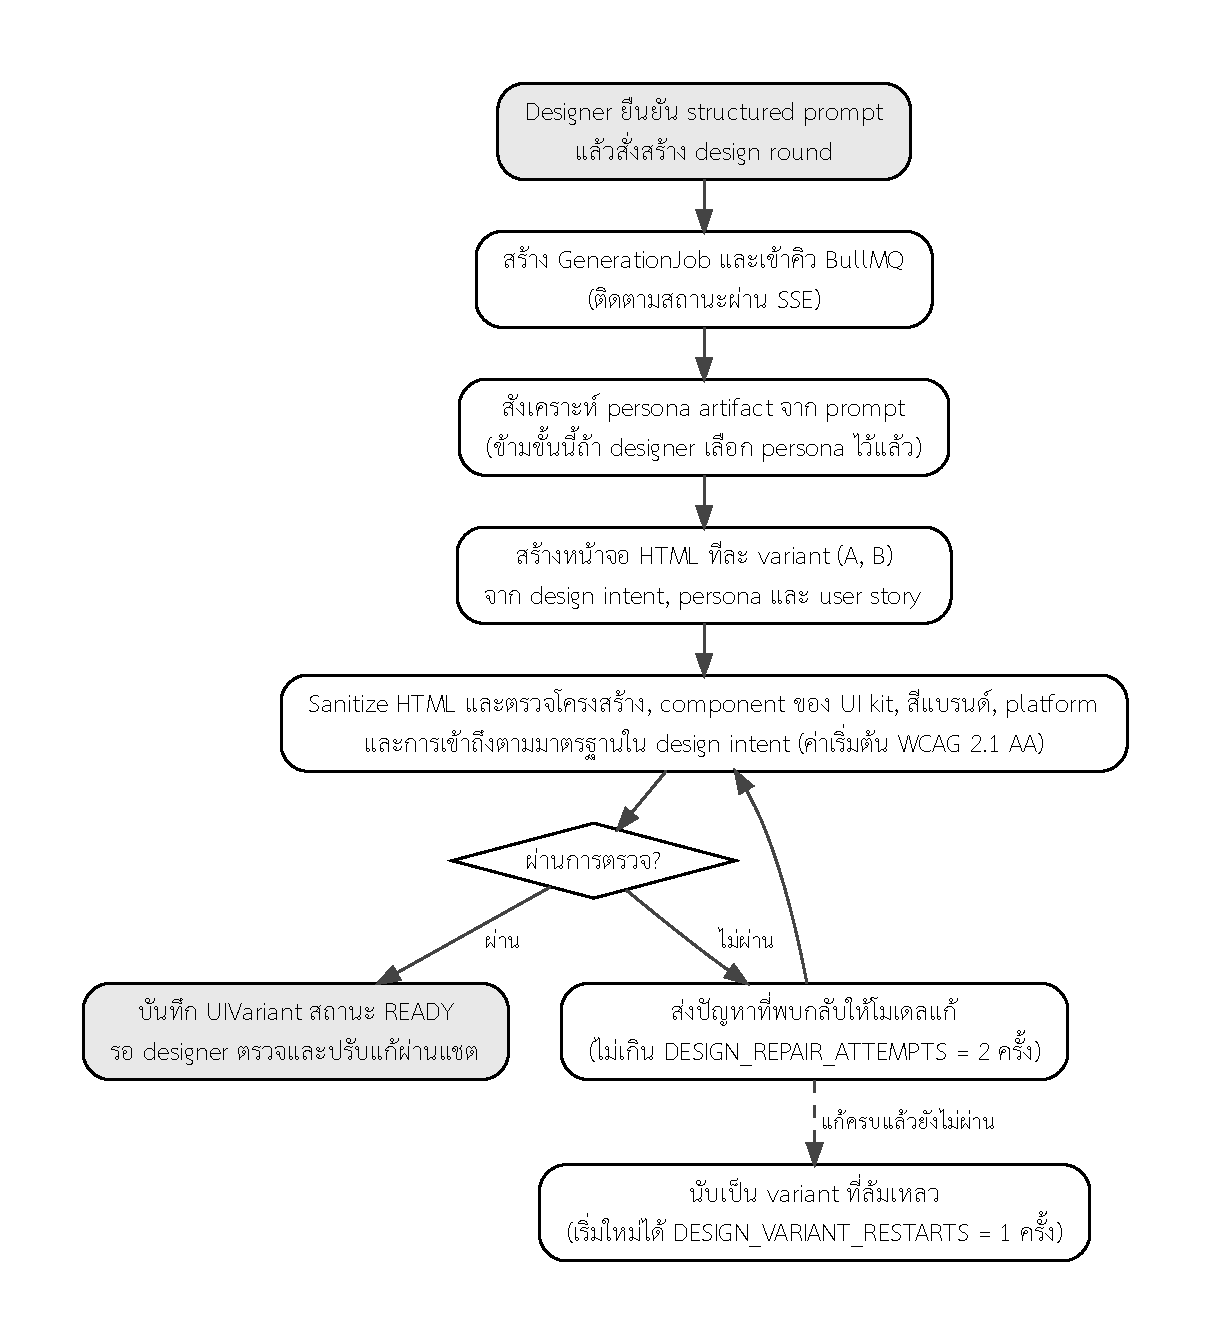
\includegraphics[width=0.78\linewidth]{figures/ch3-methodology/generation-pipeline.pdf}
  \caption{ขั้นตอนการสร้าง UI variant ด้วย AI}
  \label{fig:generation-pipeline}
\end{figure}

\subsection{Generation Trace}
\thaijustify{
  ระหว่างสร้าง UI หน้าจอแสดงความคิดของโมเดลและสถานะของแต่ละขั้นแบบ real-time ผ่าน SSE พร้อมเวลาที่ใช้จริงและผลการตรวจจริงของแต่ละ variant รอบการแก้ไขภายในจะไม่แสดงให้ผู้ใช้เห็น เพื่อให้ trace อ่านง่าย และหาก backend เริ่มสร้าง variant ใหม่ trace จะติดตามงานใหม่ต่อโดยอัตโนมัติ
  \todo{ภาพหน้าจอ generation trace}
}

\subsection{การวิเคราะห์ข้อเสนอแนะของผู้ใช้ (Backend)}
\thaijustify{
  backend รองรับการให้โมเดลวิเคราะห์ข้อเสนอแนะและพฤติกรรมของผู้เข้าร่วมทดสอบ แล้วจัดกลุ่มเป็นประเด็น (theme) ให้นักออกแบบเลือกไปเริ่มรอบการออกแบบถัดไป ข้อมูลส่วนบุคคลถูกลบออกก่อนส่งให้โมเดล หน้าจอของส่วนนี้อยู่ในแผนของภาคการศึกษาที่ 2
  \todo{ชุดข้อมูลและผลการประเมินคุณภาพผลลัพธ์ของ AI}
}

% !TeX root = ../../progress-sem1.tex
% 3.x การพัฒนาระบบ: work done in semester 1 (M0-M3)
\section{การพัฒนาระบบ}
\thaijustify{
  ในภาคการศึกษาที่ 1 การพัฒนาระบบดำเนินการตาม milestone M0 ถึง M3 โดยใช้ GitHub เป็นที่เก็บซอร์สโค้ด ทุกการเปลี่ยนแปลงผ่าน pull request และตั้งชื่อตามรูปแบบ conventional commit จนถึงวันที่ 26 พฤศจิกายน 2569 มีการ commit ทั้งหมด 178 ครั้ง รายละเอียดของแต่ละ milestone มีดังนี้
}

\subsection{M0: Foundation}
\thaijustify{
  ช่วง Foundation เป็นการวางโครงสร้างพื้นฐานของโปรเจกต์ ได้แก่
  \begin{itemize}
    \item \textbf{โครงสร้างซอร์สโค้ด}\\
      monorepo ที่มี frontend และ backend ใช้คำสั่งเดียวในการรัน build, lint และ test ทั้งระบบ
    \item \textbf{สภาพแวดล้อมสำหรับพัฒนา}\\
      ใช้ Docker Compose รัน PostgreSQL และ Redis มีสคริปต์สร้างไฟล์ตั้งค่า สร้างผู้ใช้ทดสอบ และออก token สำหรับทดสอบ API โดยไม่ต้องเข้าสู่ระบบผ่าน Google
    \item \textbf{Data model}\\
      ออกแบบ schema ของฐานข้อมูลครอบคลุมทุก milestone ตั้งแต่ผู้ใช้จนถึงรายงาน (หัวข้อ~\ref{sec:er-diagram}) และจัดการการเปลี่ยนแปลงด้วย migration ซึ่งมีทั้งหมด 7 ชุด โดยกำหนดให้ migration ที่ merge แล้วแก้ไขไม่ได้ เพื่อให้ฐานข้อมูลของทุกคนตรงกัน
    \item \textbf{Design system}\\
      ใช้ shadcn/ui เป็นพื้นฐานของหน้าจอแพลตฟอร์ม และเตรียม UI kit สองชุด คือ shadcn/ui และ MUI ให้ AI ใช้สร้างหน้าจอตามที่นักออกแบบเลือก
    \item \textbf{PDPA}\\
      ออกแบบการเก็บความยินยอมของผู้เข้าร่วมทดสอบพร้อมเวอร์ชันของข้อความ เพื่อใช้ใน M4
    \item \textbf{CI}\\
      GitHub Actions ตรวจทุก pull request โดยเรียงเป็นสามขั้น คือ ชื่อ pull request, lint และ build
  \end{itemize}
  ส่วนที่ยังไม่ได้ทำคือการ deploy อัตโนมัติ (CD) และระบบเก็บ event analytics
}

\subsection{M1: Secure Access}
\thaijustify{
  ระบบยืนยันตัวตนปัจจุบันใช้การเข้าสู่ระบบด้วยบัญชี Google ผ่าน OAuth 2.0 เมื่อเข้าสู่ระบบสำเร็จ backend ออก access token แบบ JWT ที่มีอายุ 15 นาที และ refresh token ที่มีอายุ 30 วัน refresh token ถูกเก็บเป็นค่า hash และเปลี่ยนใหม่ทุกครั้งที่ใช้ (token rotation) หากมีการนำ token ที่ถูกใช้ไปแล้วกลับมาใช้ซ้ำ ระบบจะถือว่า token รั่วไหลและยกเลิก token ทั้งกลุ่มของการเข้าสู่ระบบนั้น
}
\thaijustify{
  การควบคุมสิทธิ์ใช้แนวทาง permission-based access control กล่าวคือ แต่ละบทบาทในโปรเจกต์ (Designer, Project Manager, Client และ Developer) ได้รับชุดสิทธิ์ เช่น \texttt{design:write}, \texttt{design:approve} และ \texttt{handoff:read} และ API แต่ละเส้นตรวจเฉพาะสิทธิ์ที่ต้องใช้ ไม่ได้ตรวจชื่อบทบาทโดยตรง ทำให้ปรับสิทธิ์ของแต่ละบทบาทได้ในที่เดียว นอกจากนี้ระบบบันทึกการกระทำสำคัญลง audit log และมี end-to-end test ตรวจการควบคุมสิทธิ์
}
\thaijustify{
  หน้าจอสมัครสมาชิก เข้าสู่ระบบ และลืมรหัสผ่านพัฒนาส่วน frontend แล้ว ส่วนการสมัครด้วยอีเมลและรหัสผ่าน การยืนยันอีเมล และการรีเซ็ตรหัสผ่านฝั่ง backend อยู่ระหว่างพัฒนาใน branch แยก และจะรวมเข้า branch หลักภายในภาคการศึกษาที่ 1
}
\begin{figure}[H]
  \centering
  \subfloat[เข้าสู่ระบบ]{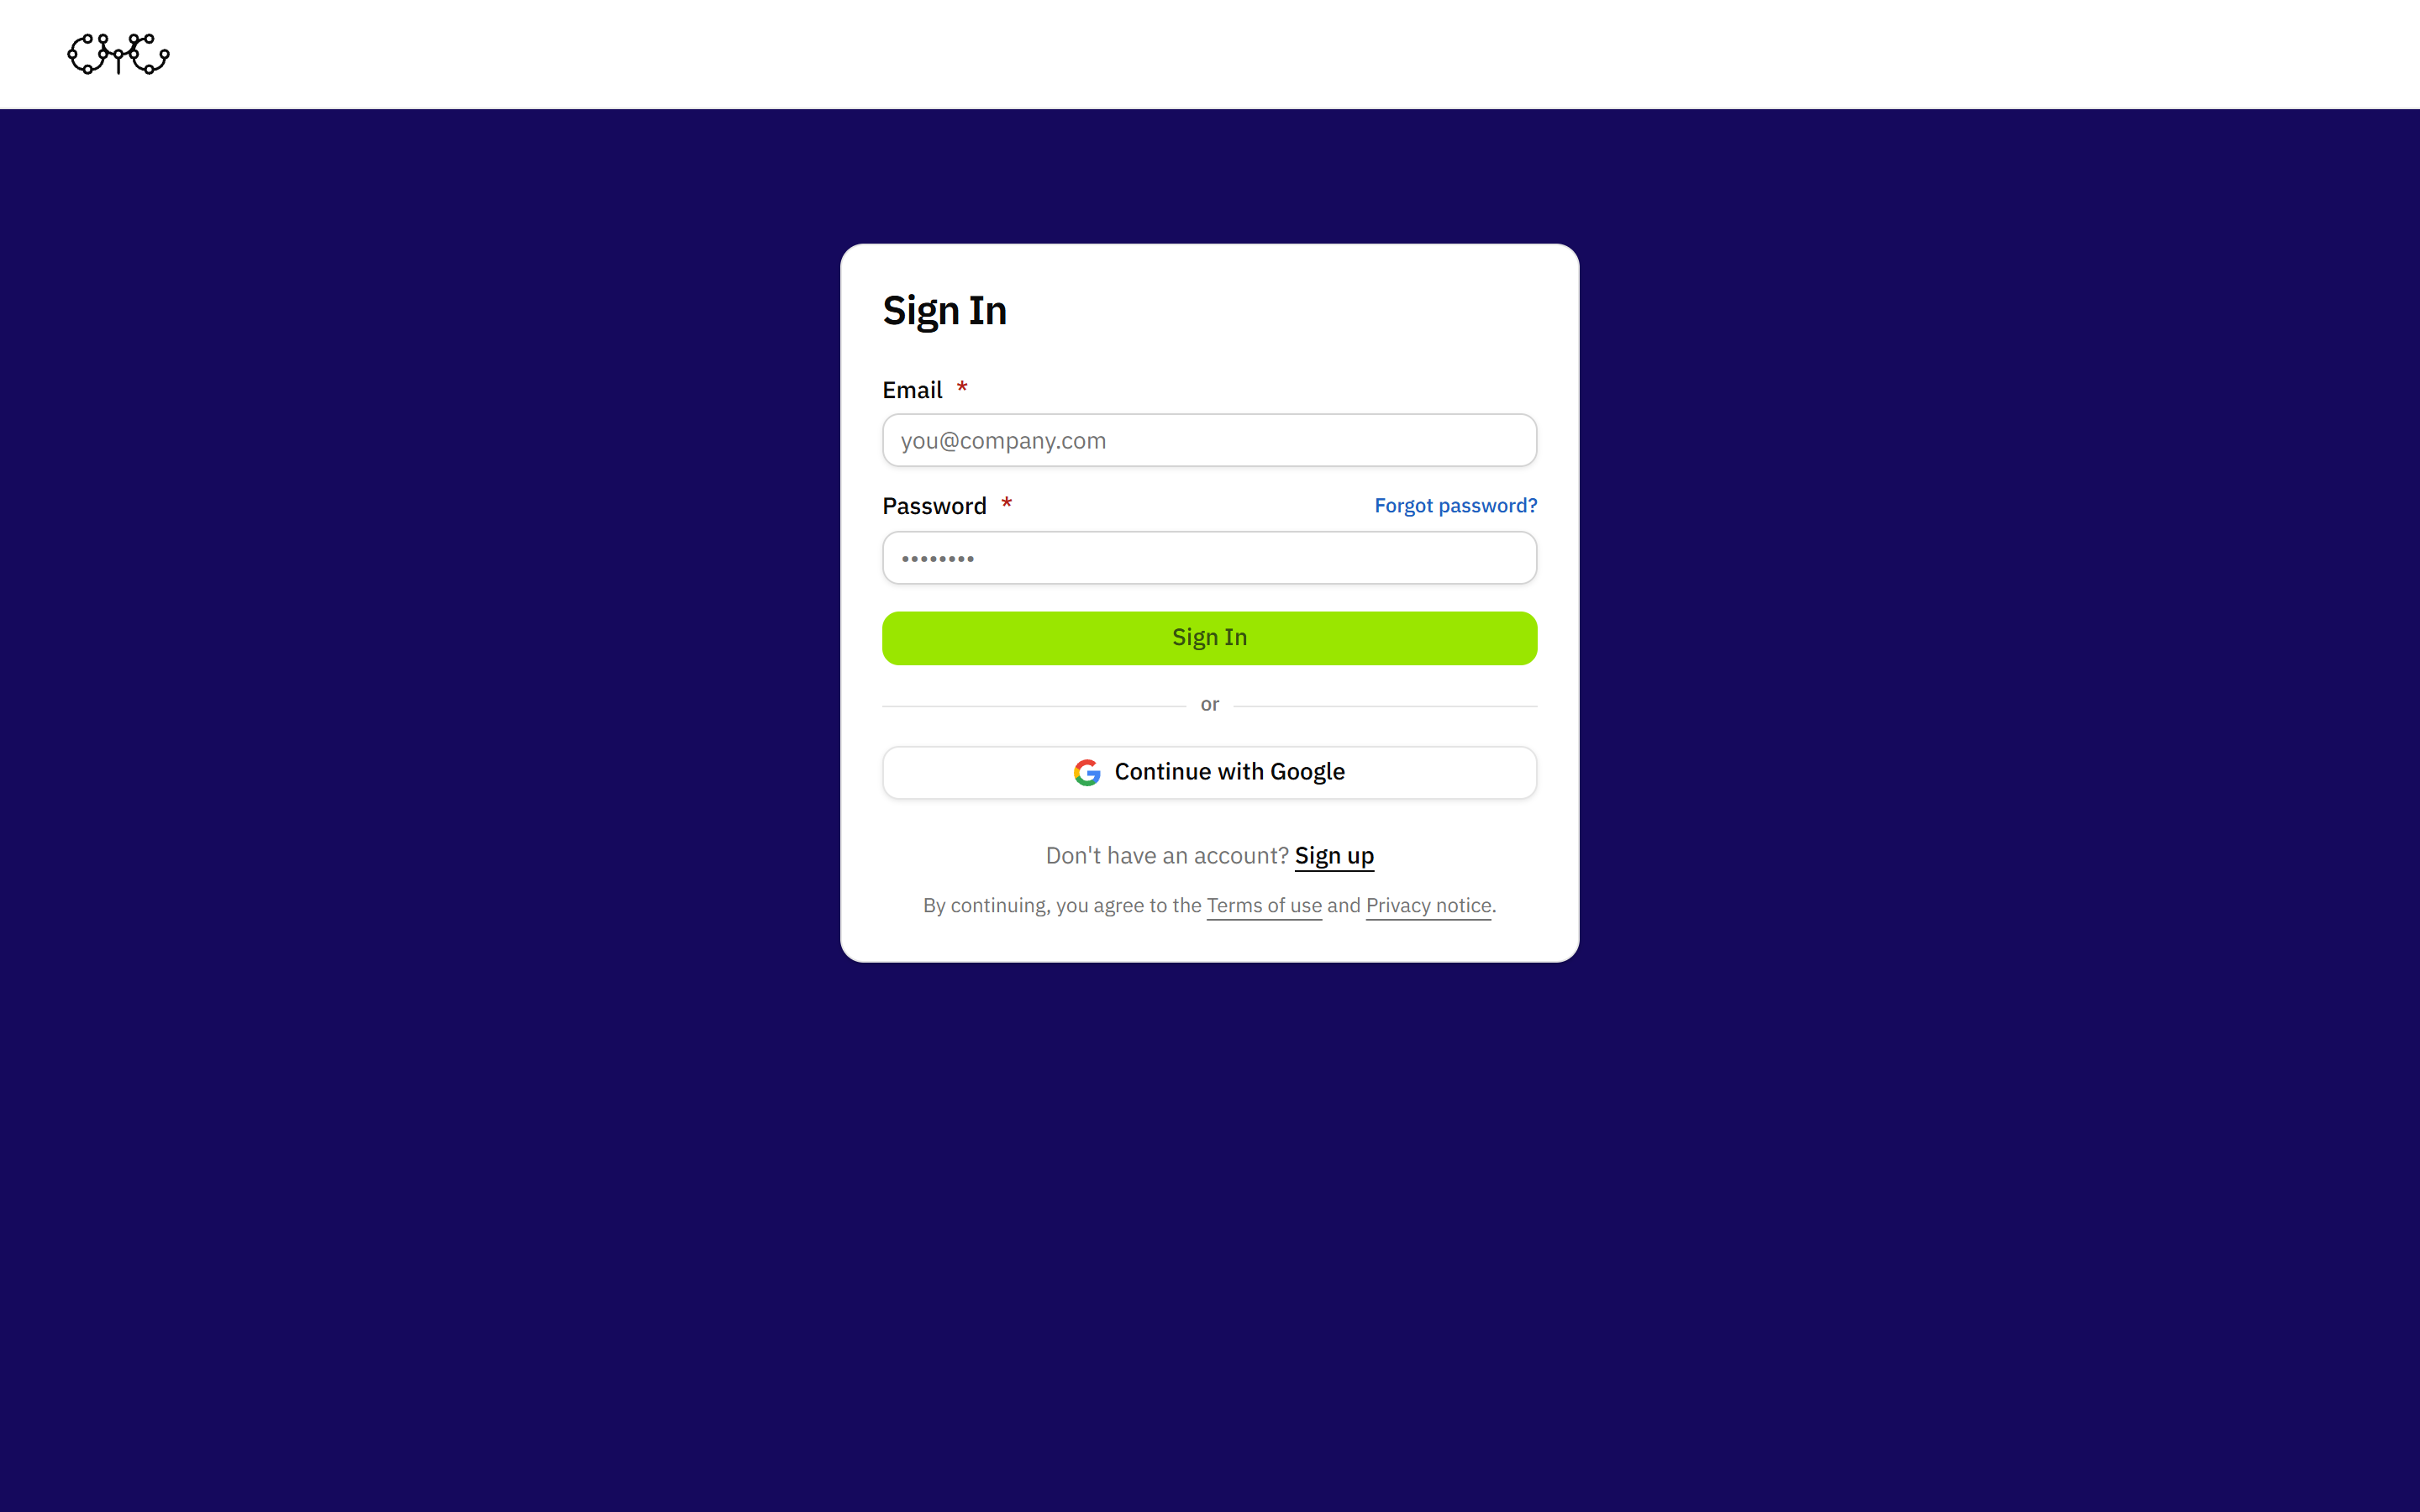
\includegraphics[width=0.49\linewidth]{figures/ch3-methodology/screens/signin.png}}\hfill
  \subfloat[สมัครสมาชิก]{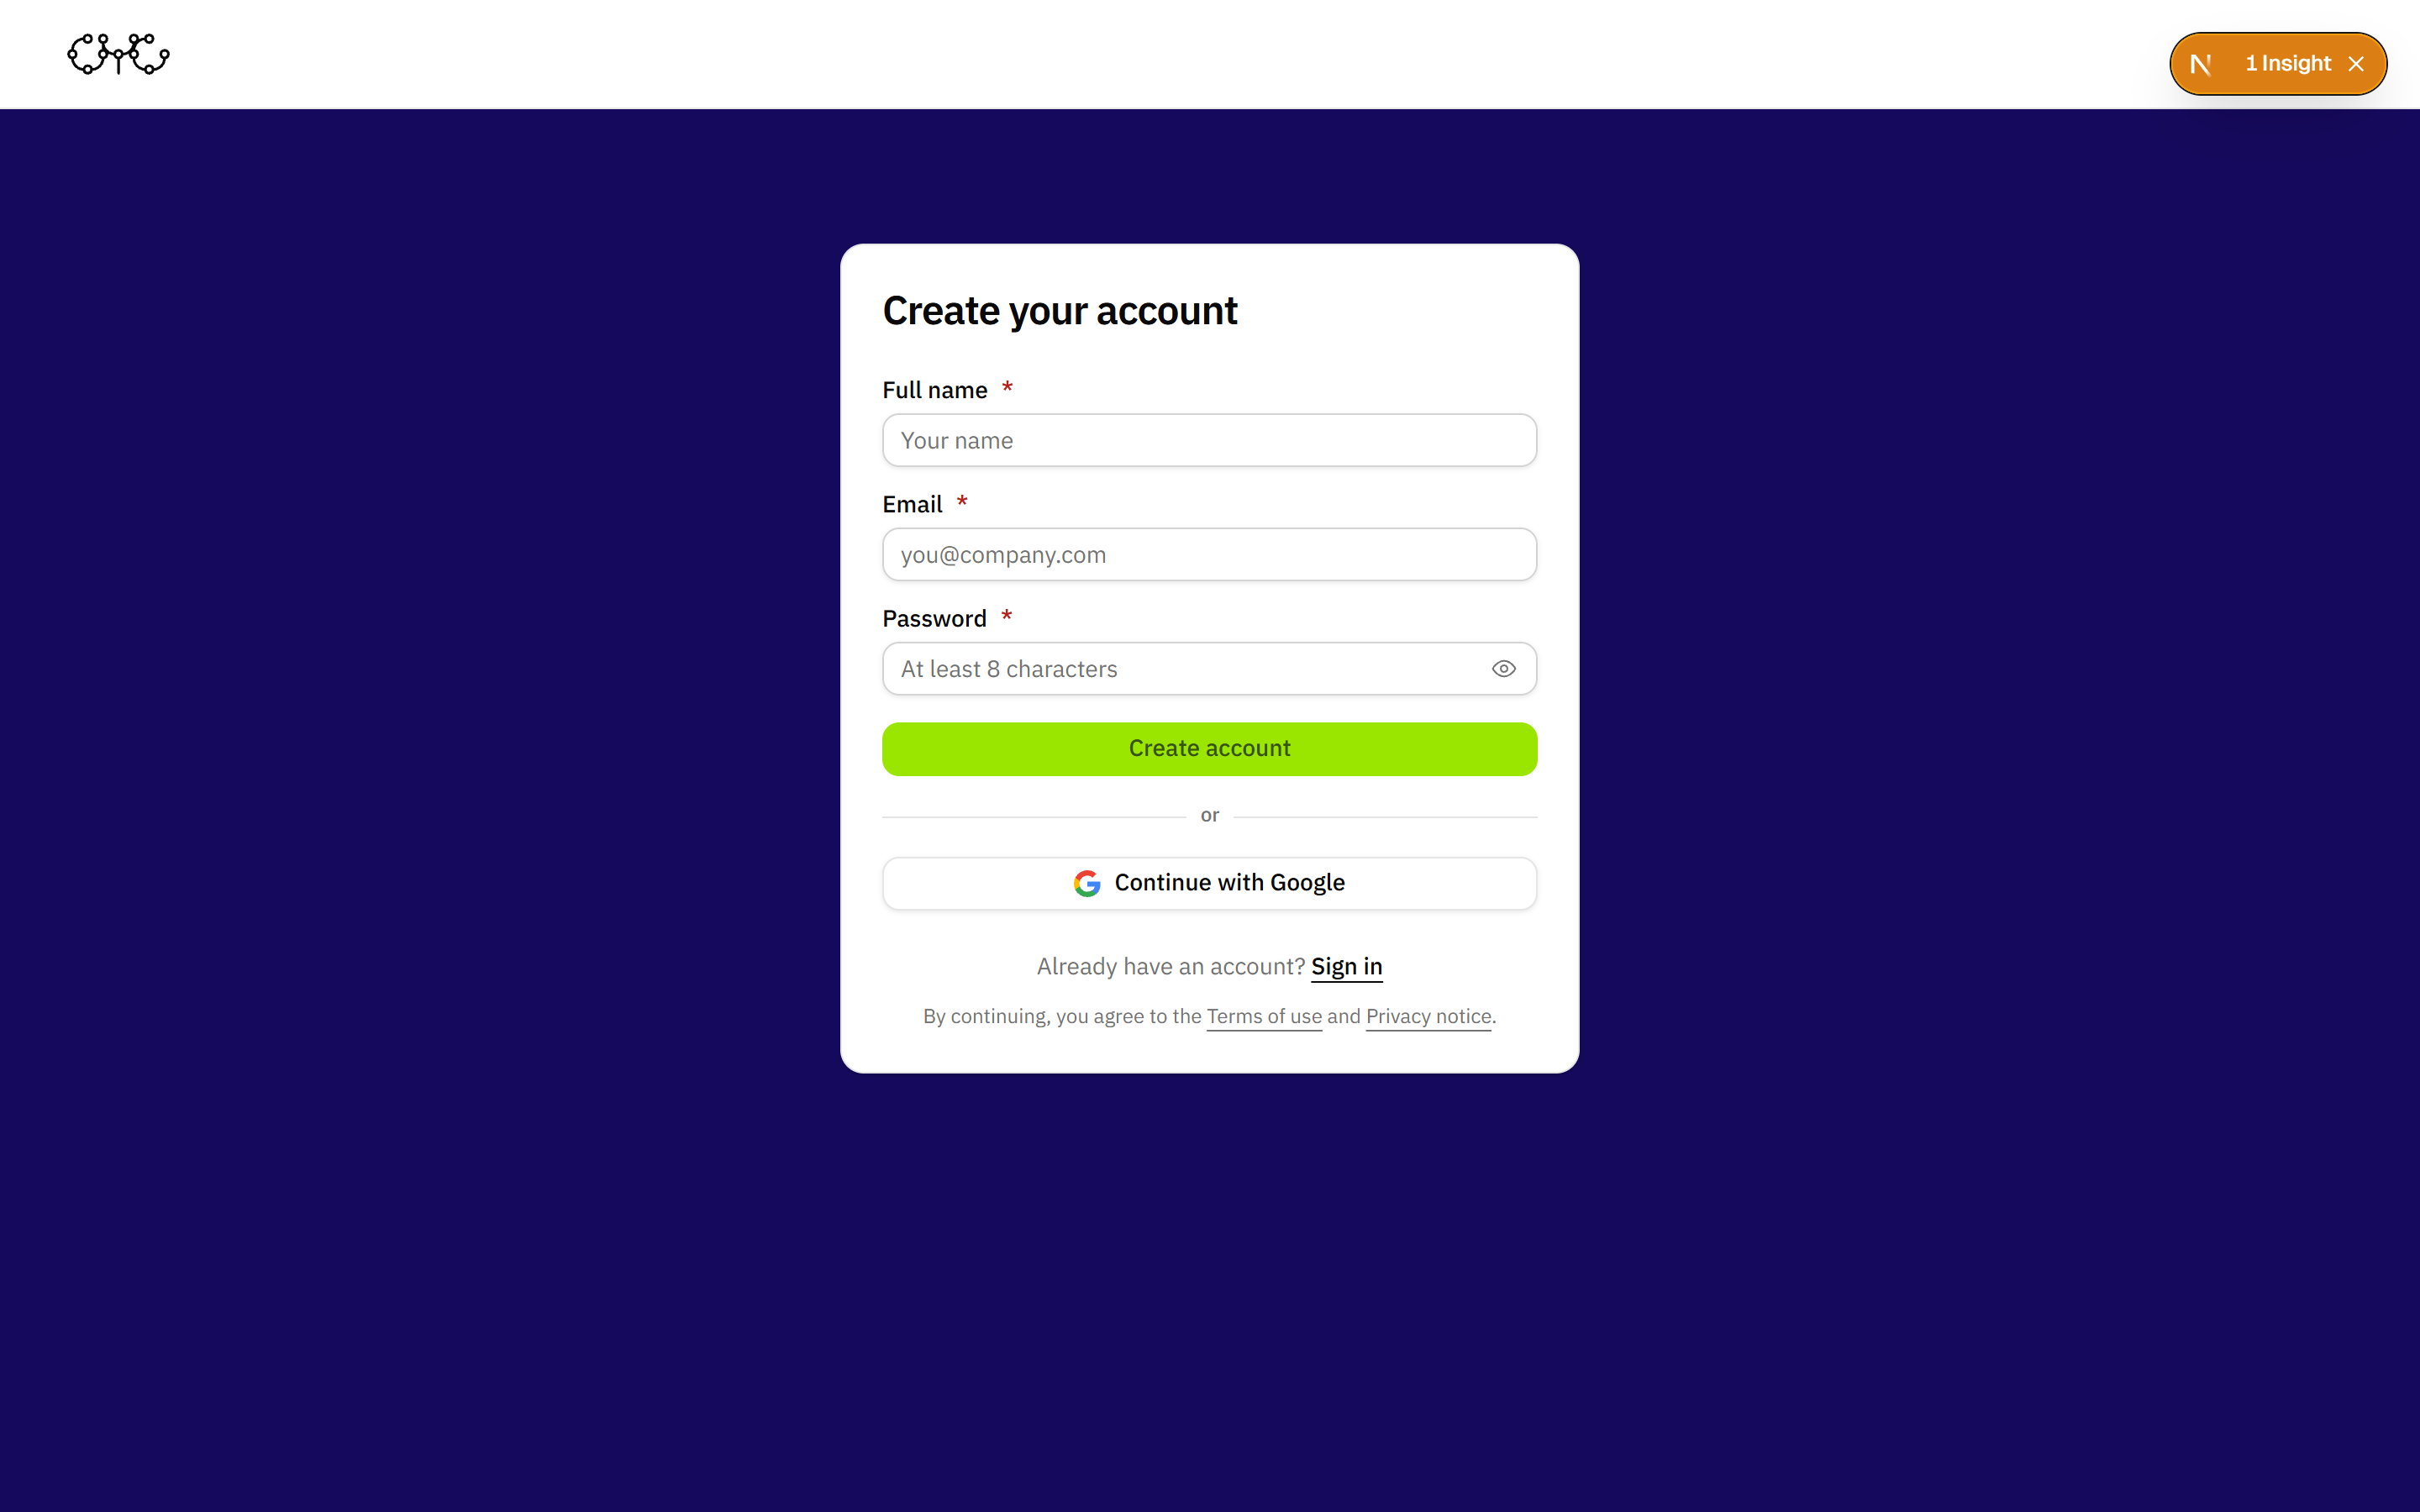
\includegraphics[width=0.49\linewidth]{figures/ch3-methodology/screens/signup.png}}
  \caption{หน้าจอเข้าสู่ระบบและสมัครสมาชิก}
  \label{fig:screen-auth}
\end{figure}

\subsection{M2: Project Setup}
\thaijustify{
  ผู้ใช้สร้าง workspace ตั้งรูปประจำ workspace และเชิญสมาชิกด้วยอีเมลได้ ภายใน workspace นักออกแบบสร้างโปรเจกต์ กำหนดสมาชิกและบทบาทในโปรเจกต์ และค้นหาหรือกรองโปรเจกต์ได้ทั้งแบบรายการและแบบแกลเลอรี
}
\thaijustify{
  ความต้องการทางการออกแบบ (design intent) ของโปรเจกต์ประกอบด้วยเป้าหมายของการออกแบบ design system ที่เลือก (shadcn/ui หรือ MUI) มาตรฐานการเข้าถึง (ค่าเริ่มต้น WCAG 2.1 AA) แนวทางการออกแบบ สีแบรนด์สามสี แนวทาง CI และ tone of voice ทุกครั้งที่แก้ไข ระบบจะเพิ่มเลขเวอร์ชันของ design intent และงานสร้าง UI แต่ละครั้งเก็บสำเนาของ design intent ที่ใช้ไว้ ทำให้ design intent เป็น context ที่ AI นำไปใช้ซ้ำได้ และตรวจสอบย้อนหลังได้ว่า UI แต่ละชุดสร้างจาก design intent ฉบับใด นอกจากนี้นักออกแบบเพิ่ม persona ของผู้ใช้เป้าหมายเองได้ และหน้าภาพรวมของโปรเจกต์แสดงกิจกรรมล่าสุดจาก audit log
}
\begin{figure}[H]
  \centering
  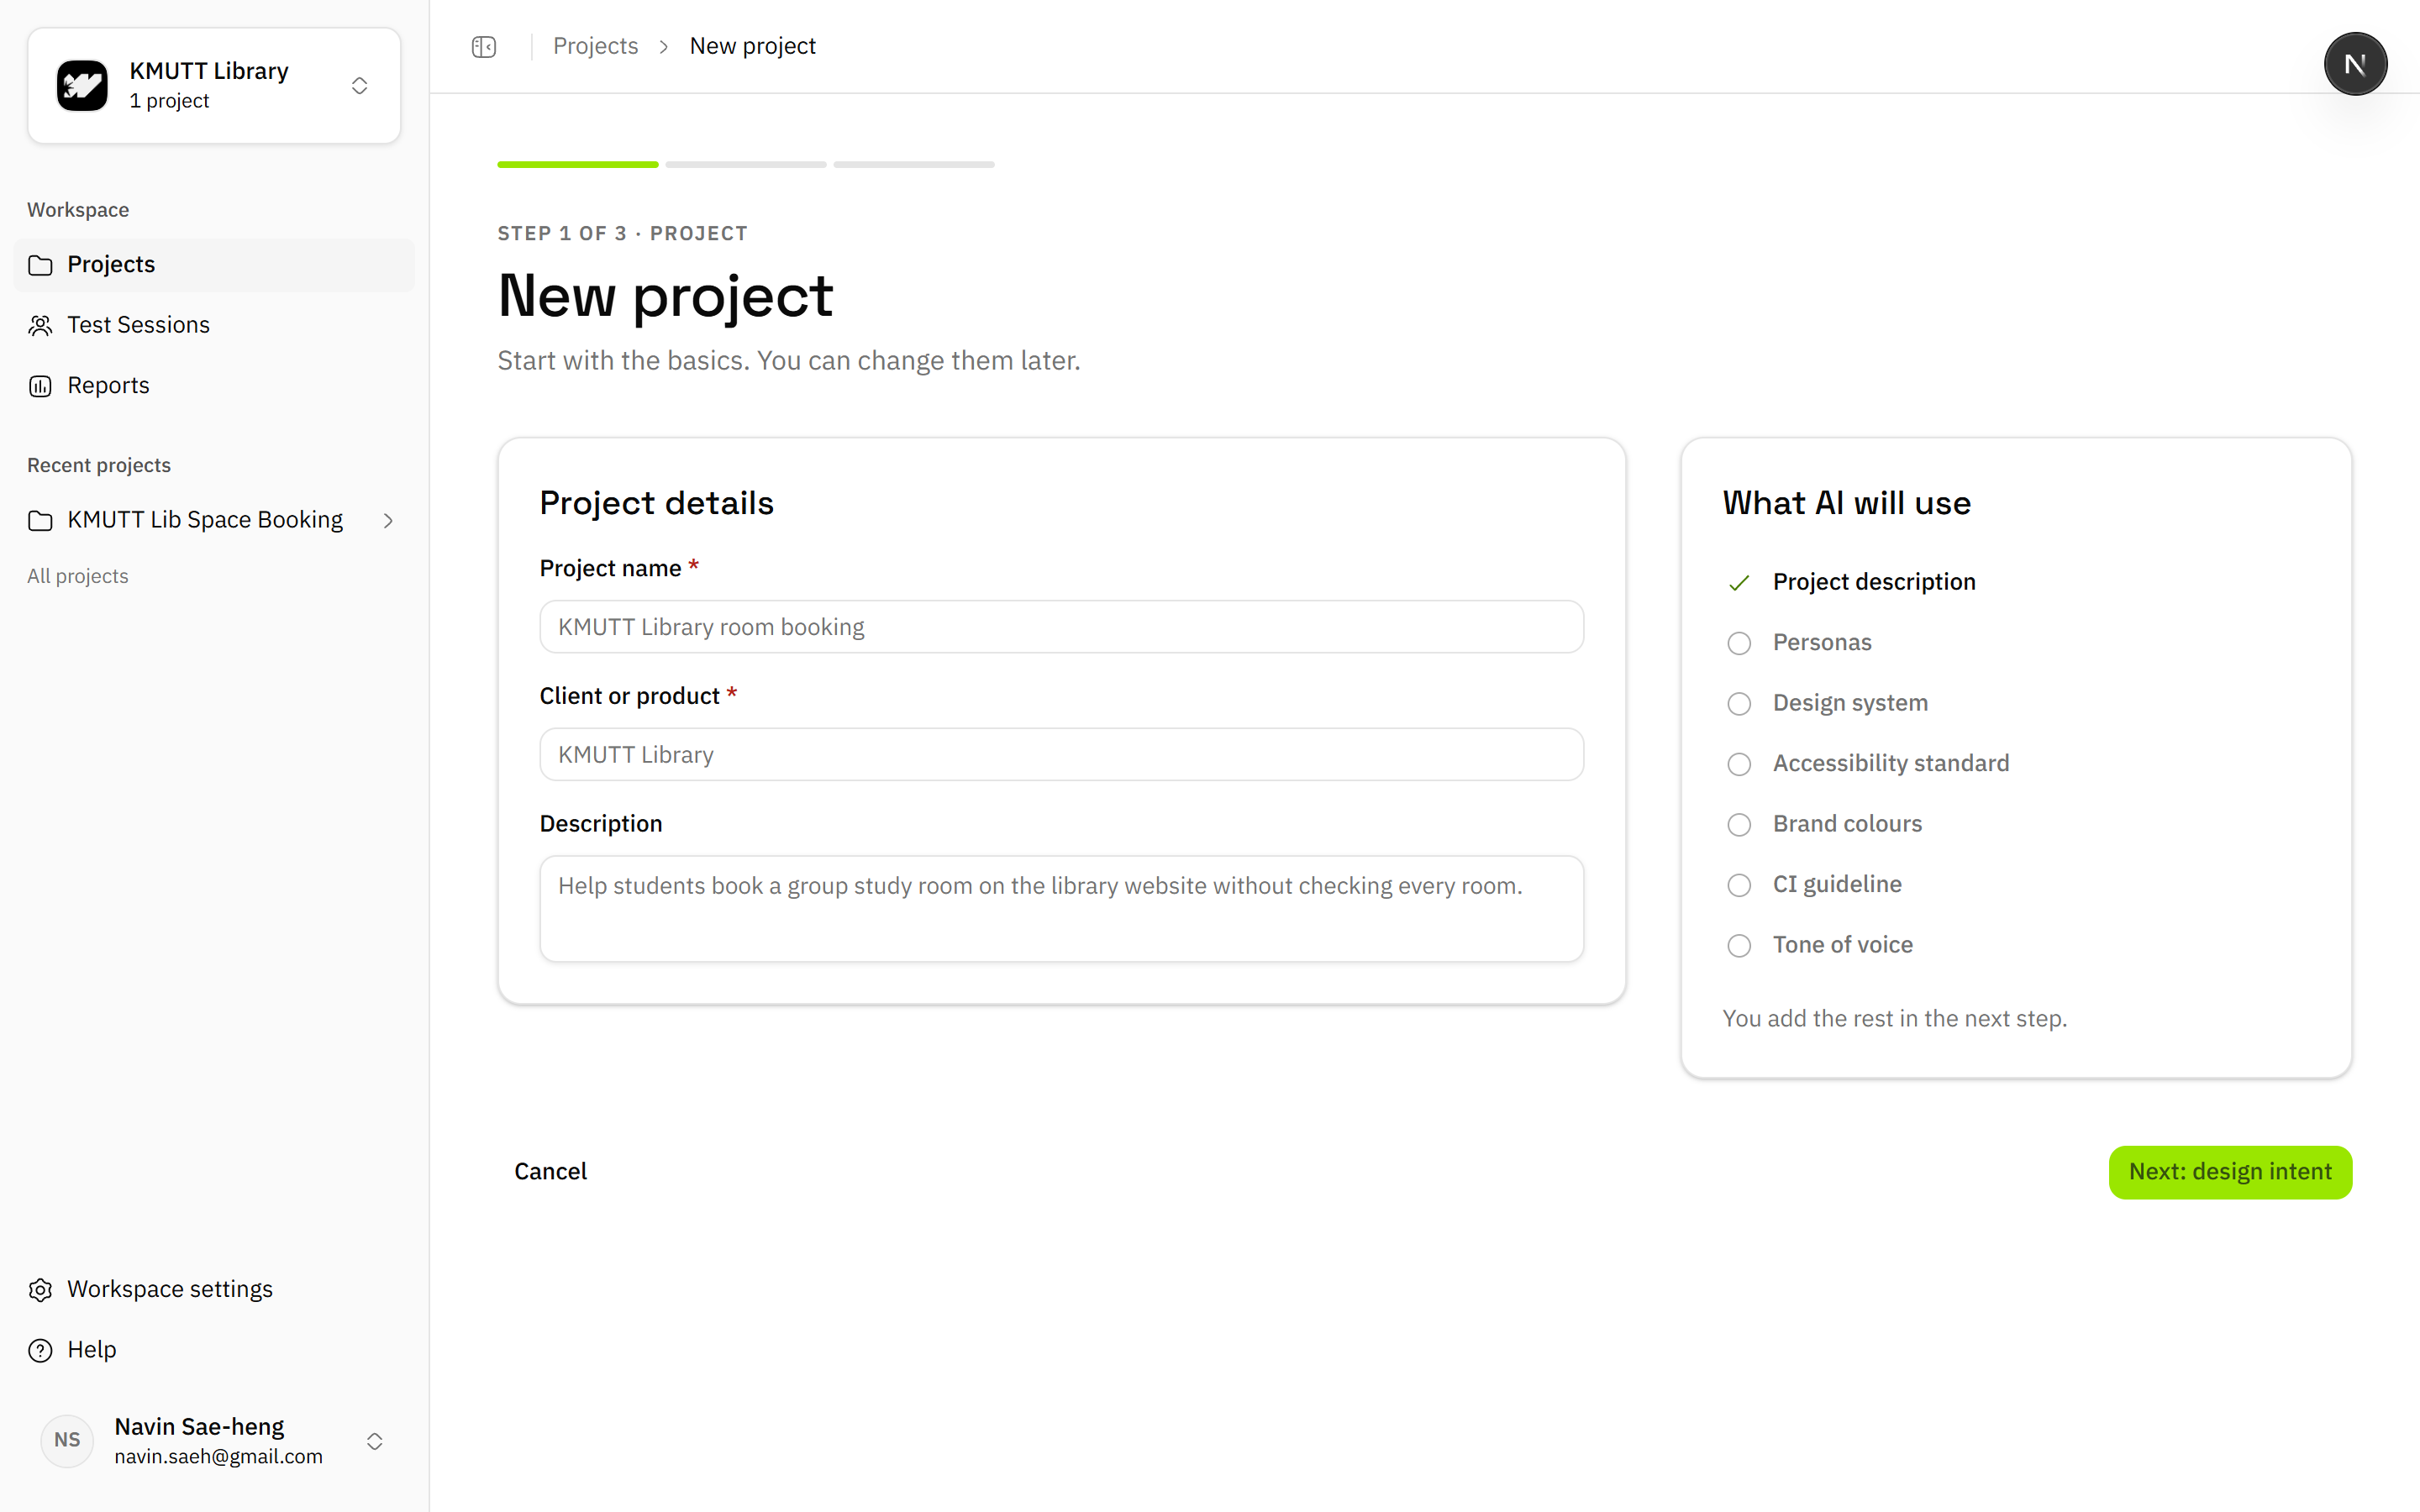
\includegraphics[width=0.9\linewidth]{figures/ch3-methodology/screens/project-new.png}
  \caption{หน้าจอสร้างโปรเจกต์ (ขั้นที่ 1 จาก 3 ของ wizard)}
  \label{fig:screen-project-new}
\end{figure}
\begin{figure}[H]
  \centering
  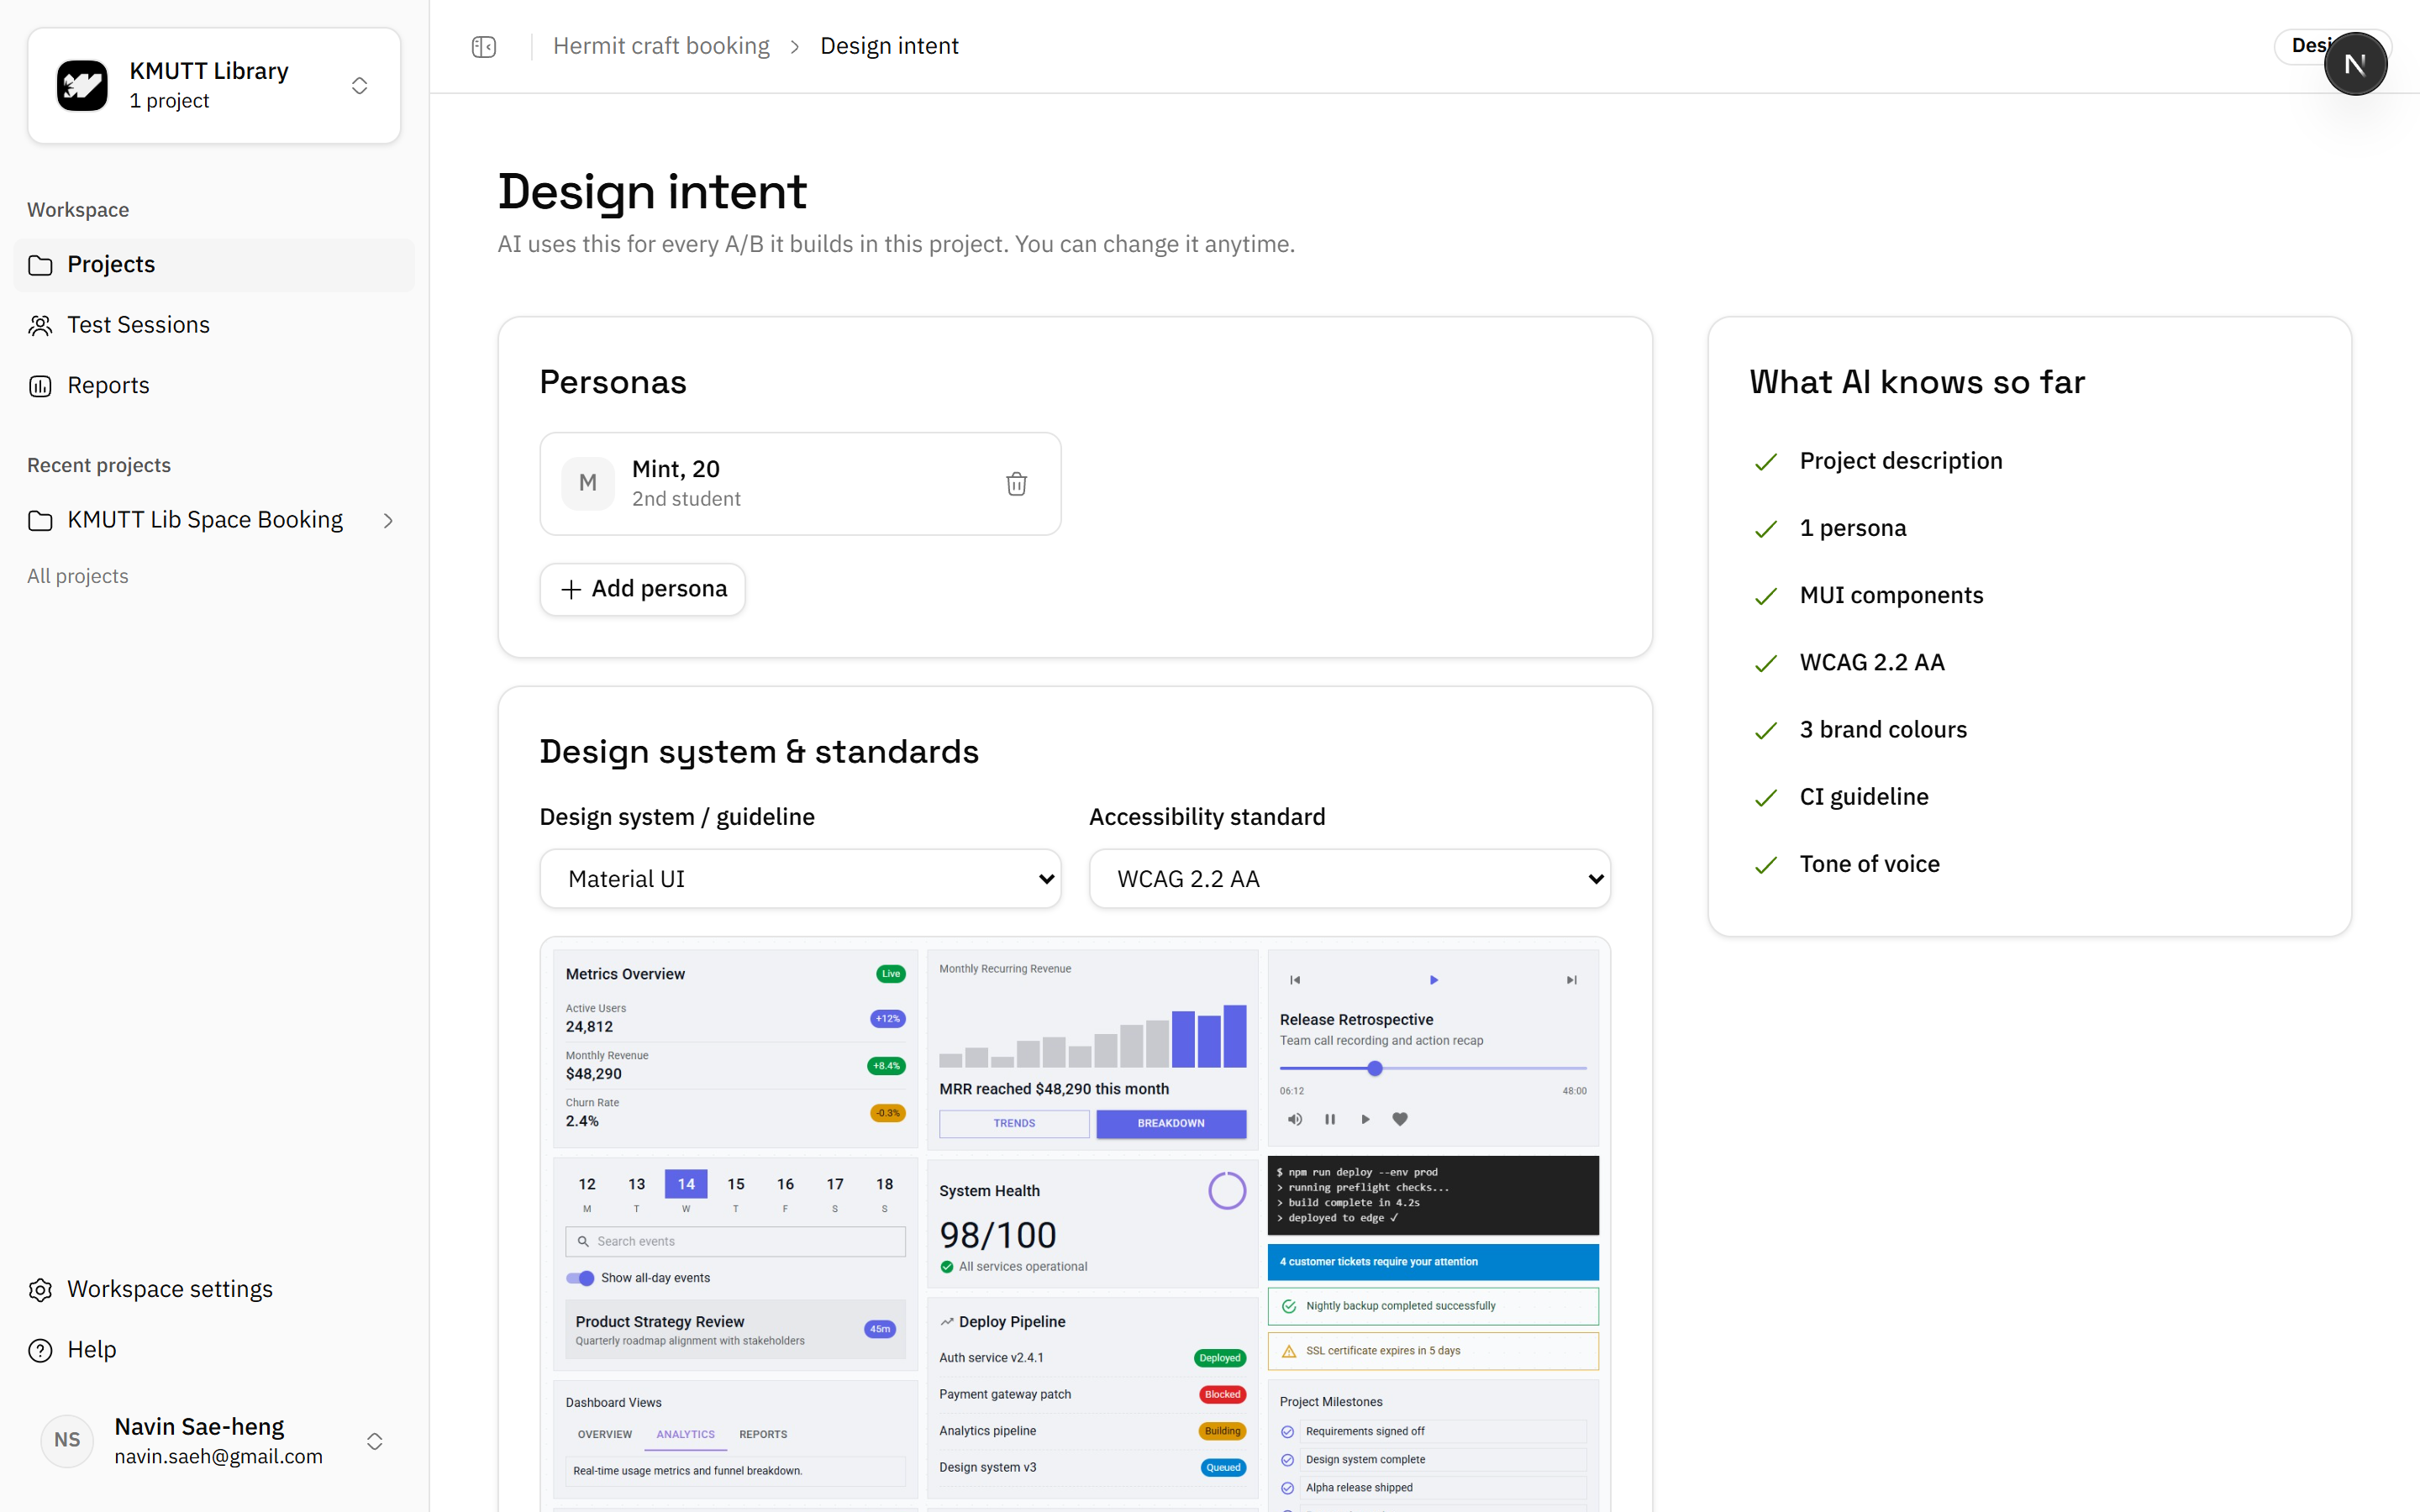
\includegraphics[width=0.9\linewidth]{figures/ch3-methodology/screens/design-intent.png}
  \caption{หน้าจอกำหนดความต้องการทางการออกแบบ (design intent)}
  \label{fig:screen-design-intent}
\end{figure}
\begin{figure}[H]
  \centering
  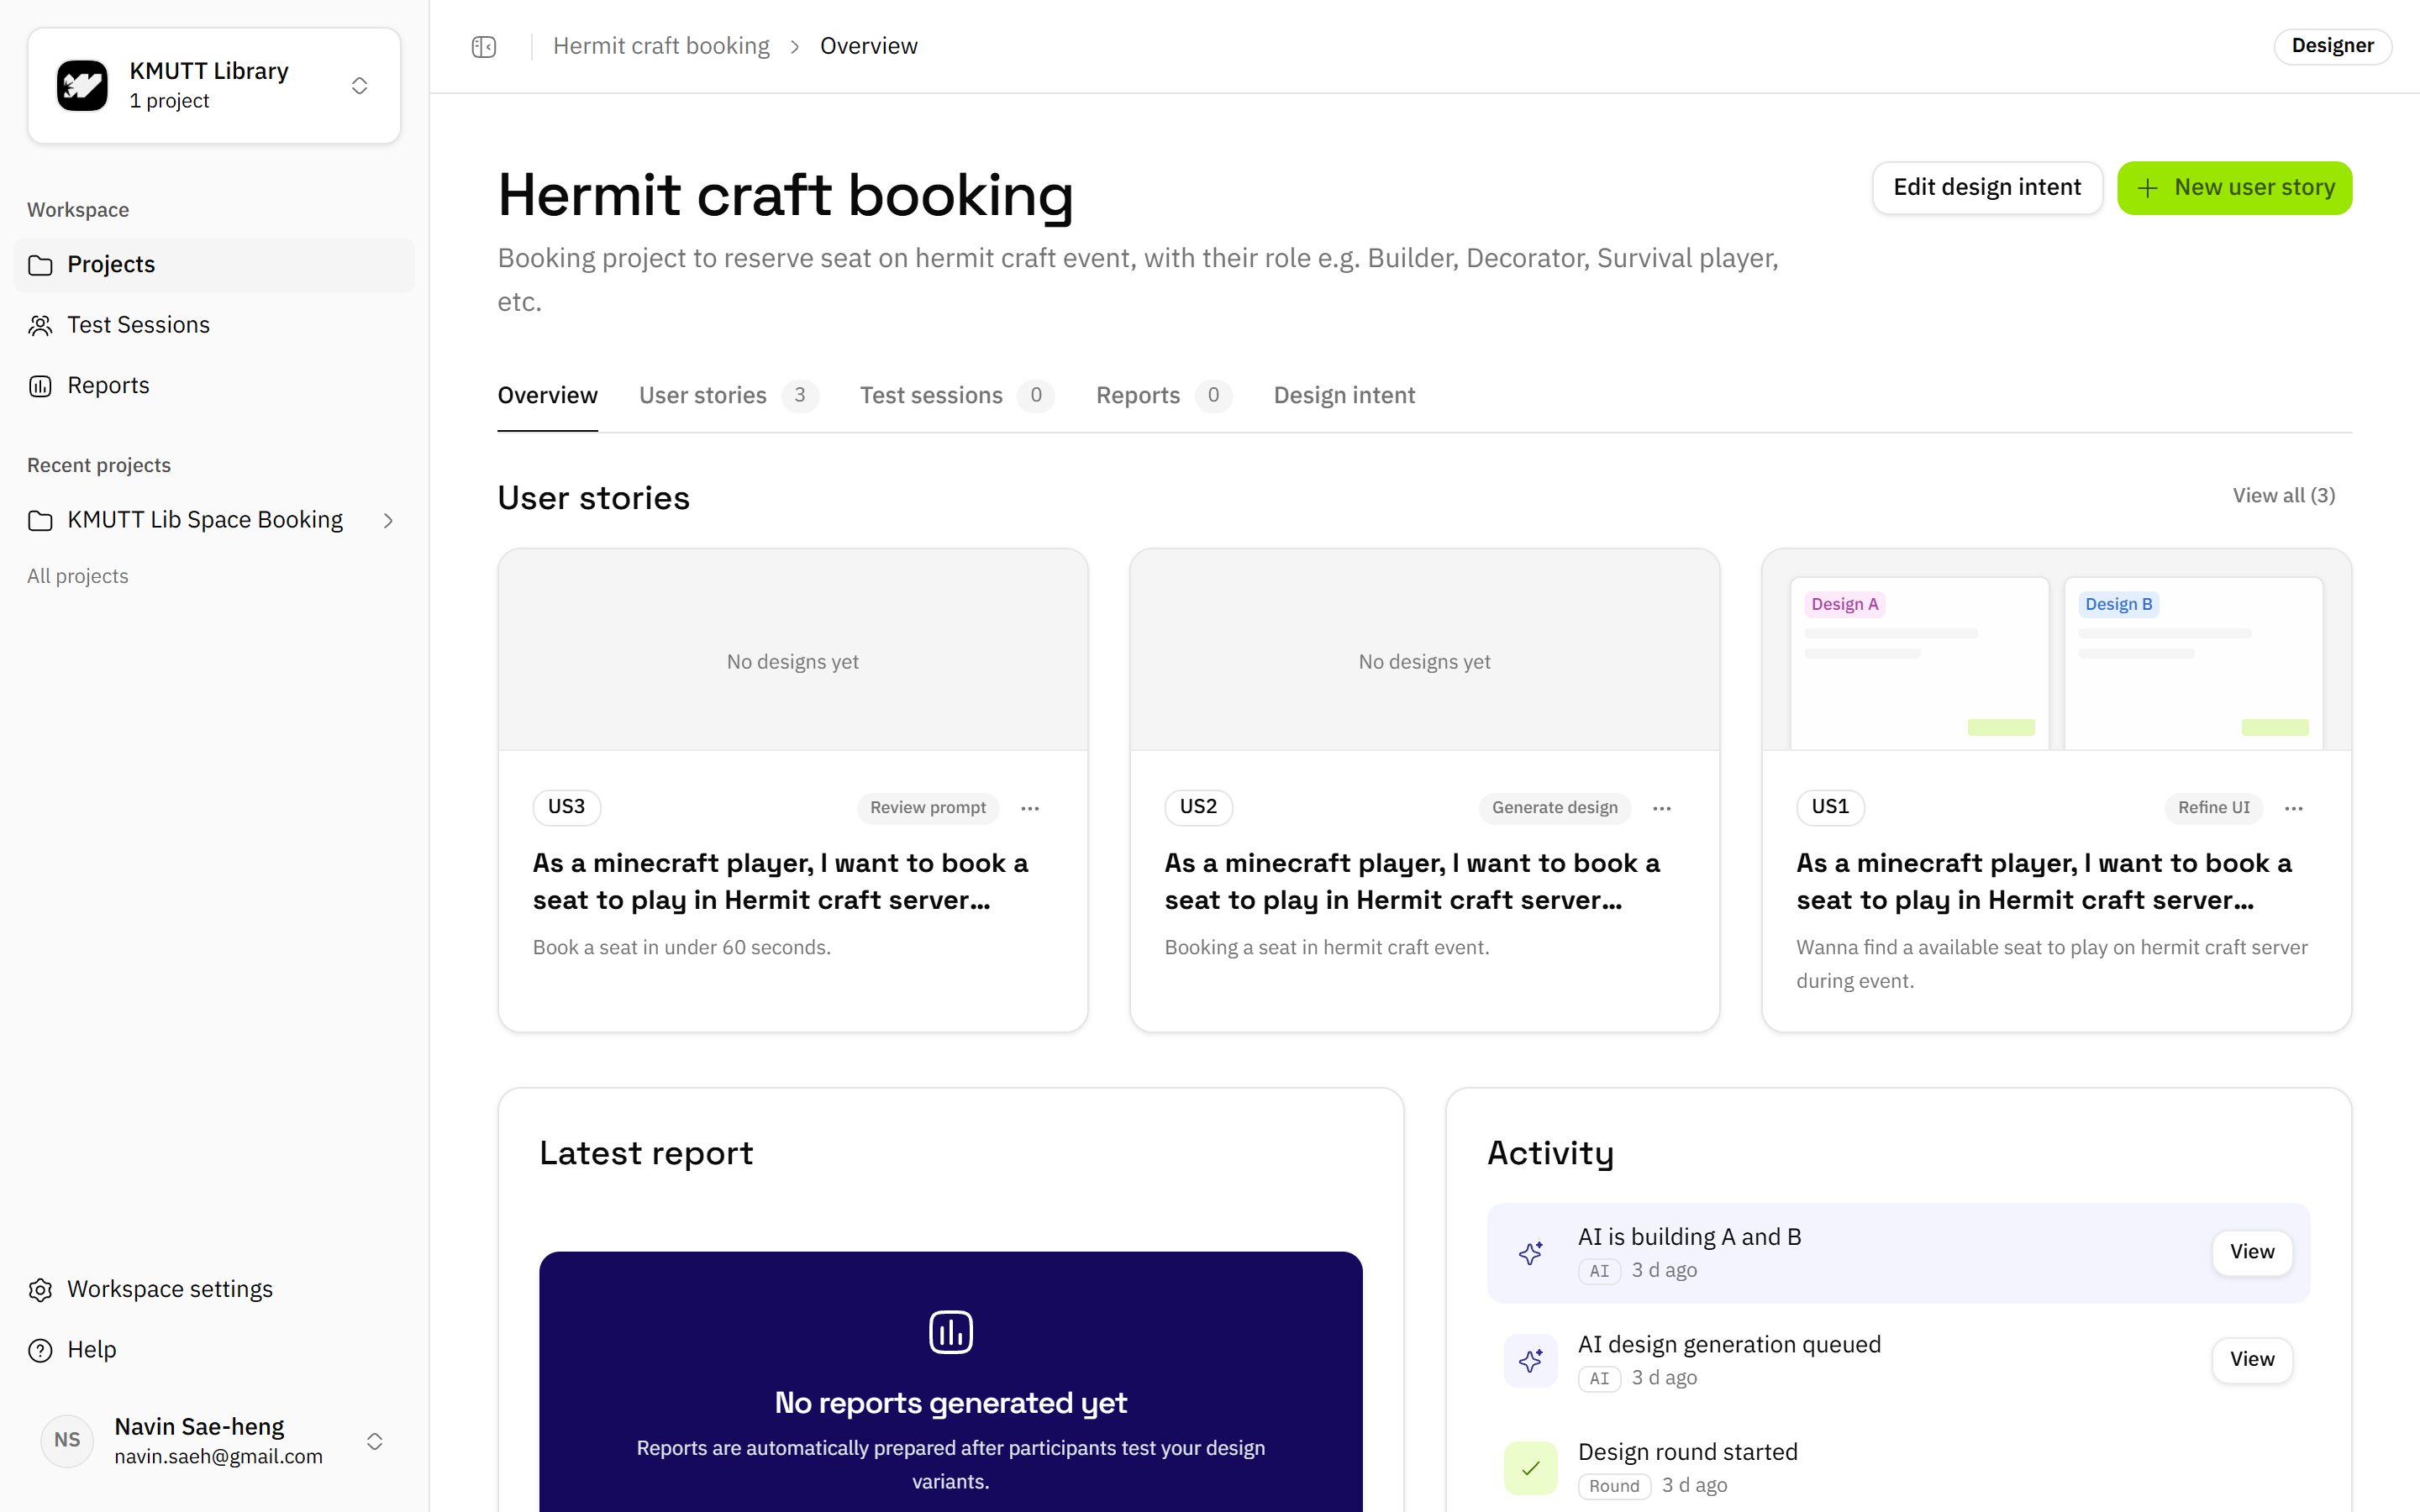
\includegraphics[width=0.9\linewidth]{figures/ch3-methodology/screens/project-overview.png}
  \caption{หน้าภาพรวมของโปรเจกต์ แสดง user story และกิจกรรมล่าสุด}
  \label{fig:screen-project-overview}
\end{figure}

\subsection{M3: AI Design Generation}
\thaijustify{
  นักออกแบบเขียน user story และ problem statement ผ่านหน้าจอ ซึ่ง backend รองรับการให้ AI ร่าง user story แล้วแต่ยังไม่มีหน้าจอสำหรับส่วนนี้ จากนั้น AI ร่าง structured prompt จาก design intent, persona และ user story และส่งผลลัพธ์พร้อมความคิดของโมเดลมาแสดงแบบ real-time ผ่าน SSE นักออกแบบเลือก persona ตรวจ และแก้ prompt ก่อนสั่งสร้าง UI (รูปที่~\ref{fig:screen-story} และ~\ref{fig:screen-prompt})
}
\begin{figure}[H]
  \centering
  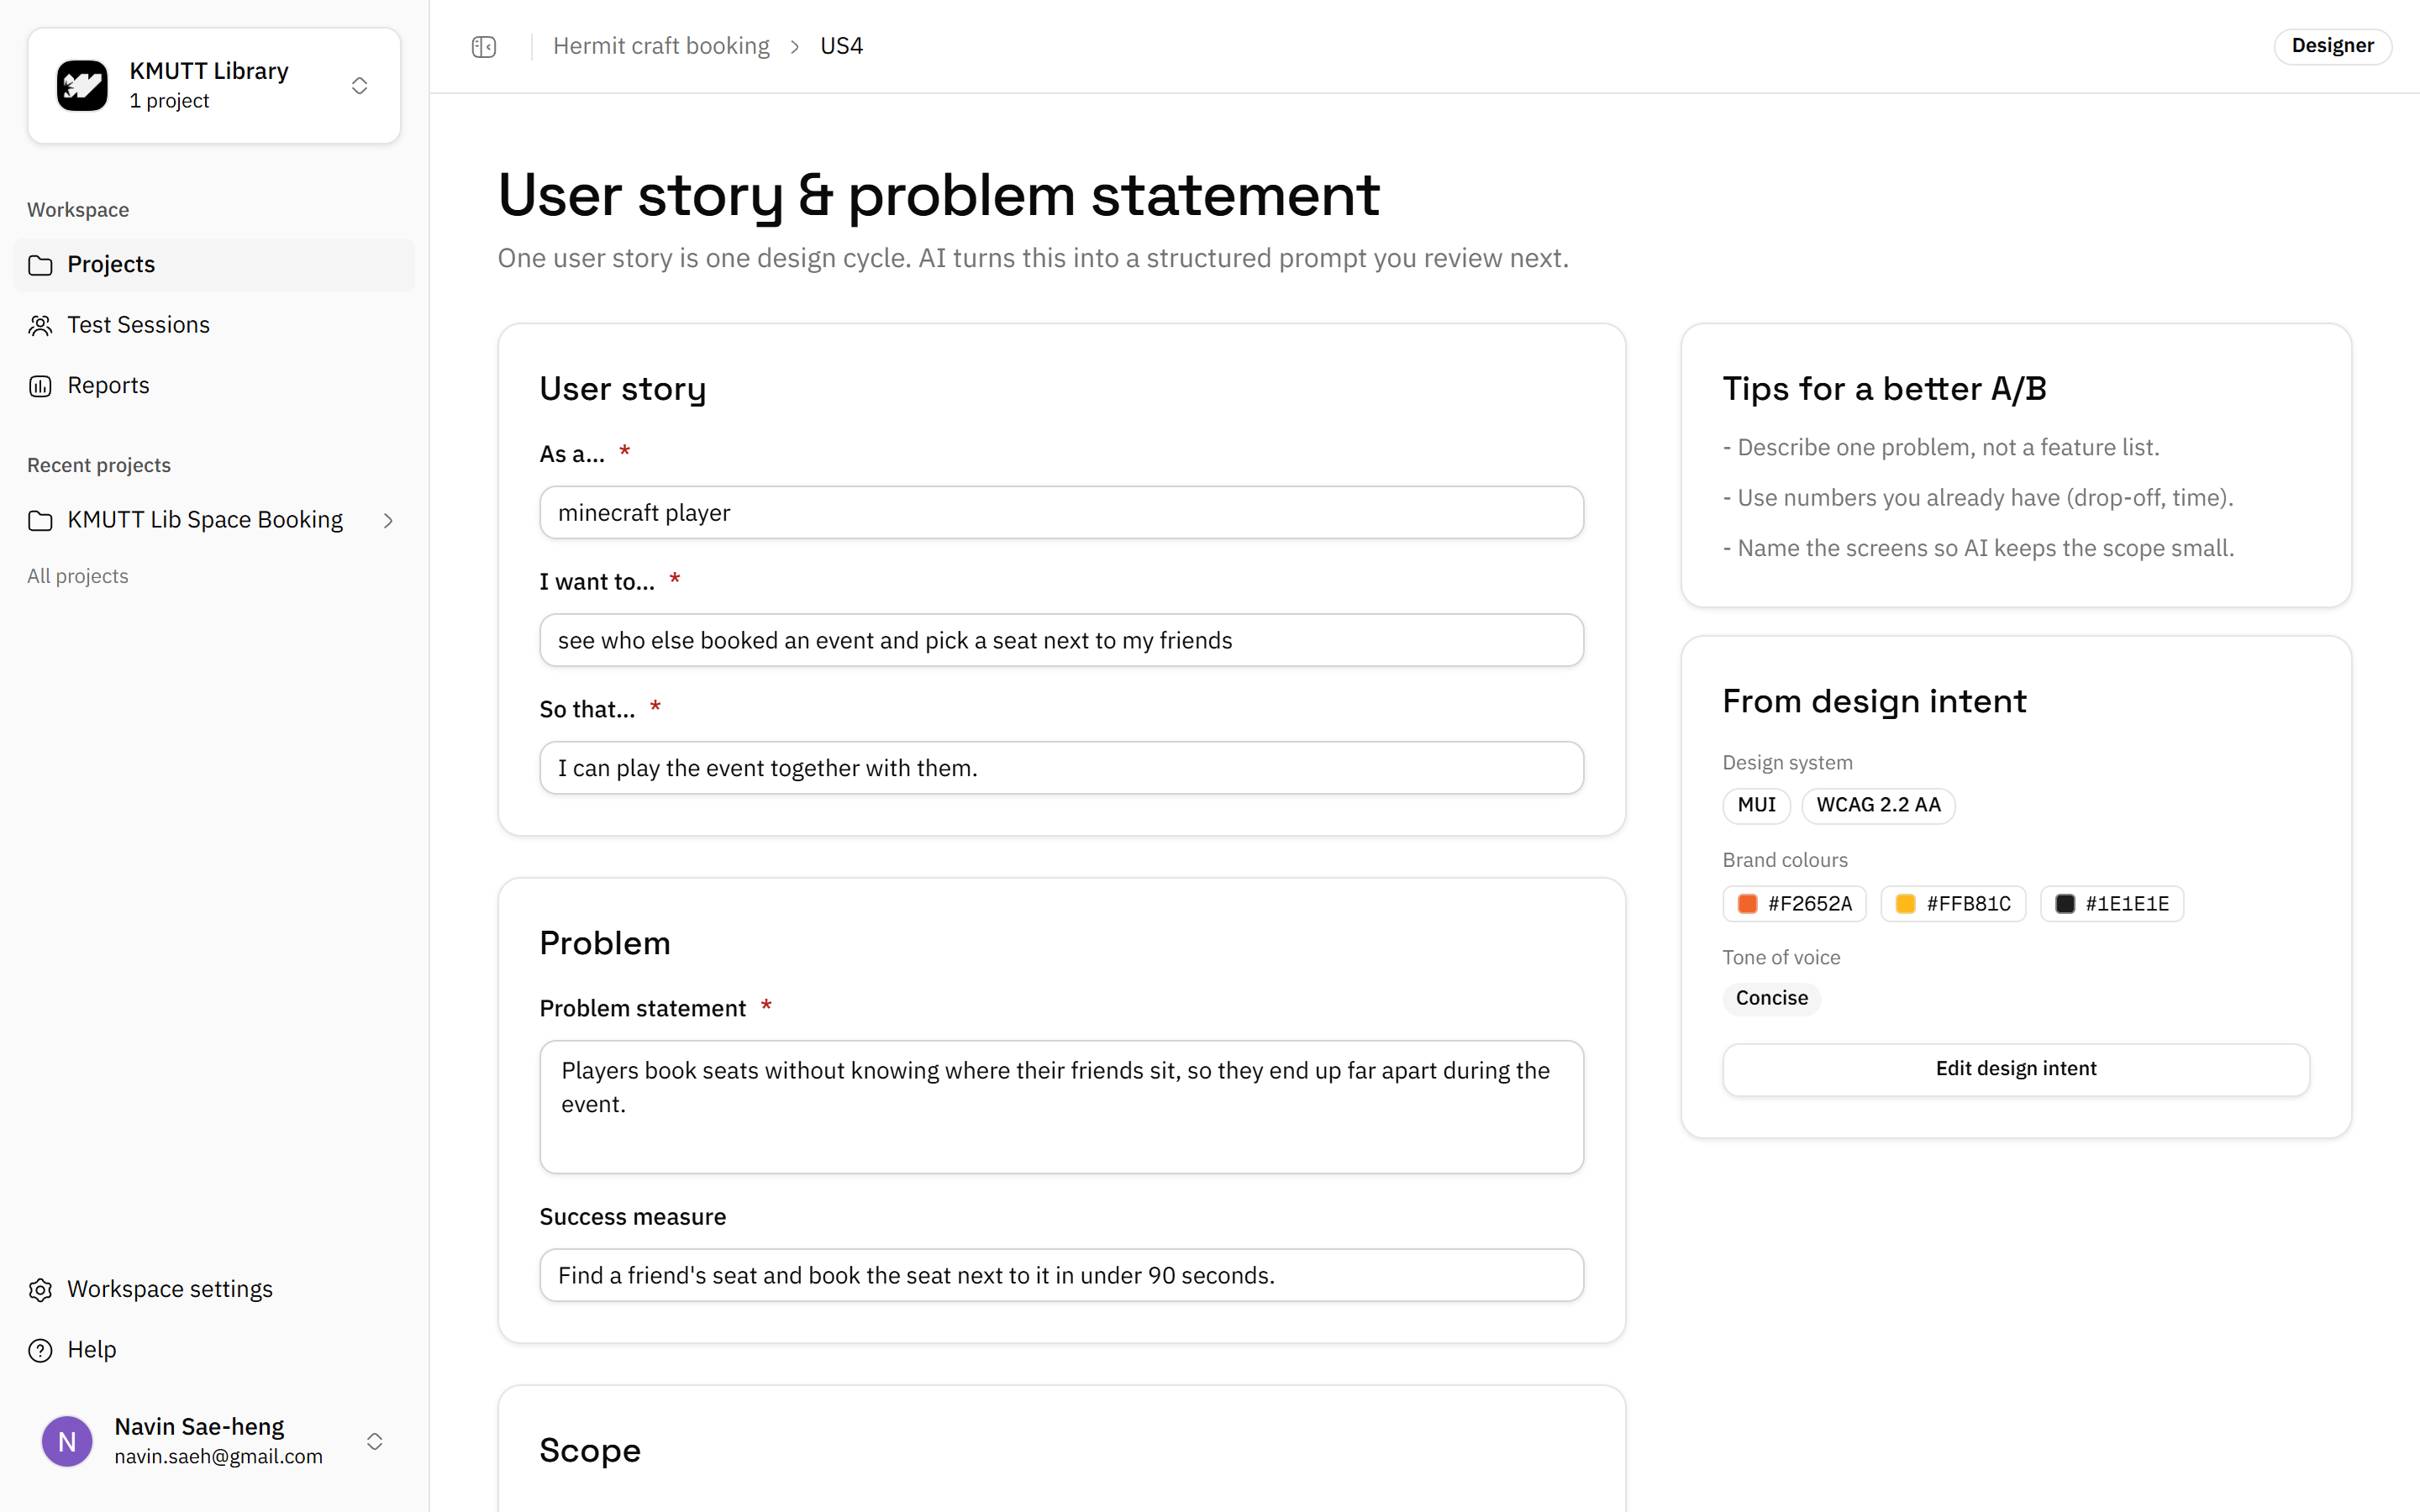
\includegraphics[width=0.9\linewidth]{figures/ch3-methodology/screens/story-us4.png}
  \caption{หน้าจอเขียน user story และ problem statement}
  \label{fig:screen-story}
\end{figure}
\begin{figure}[H]
  \centering
  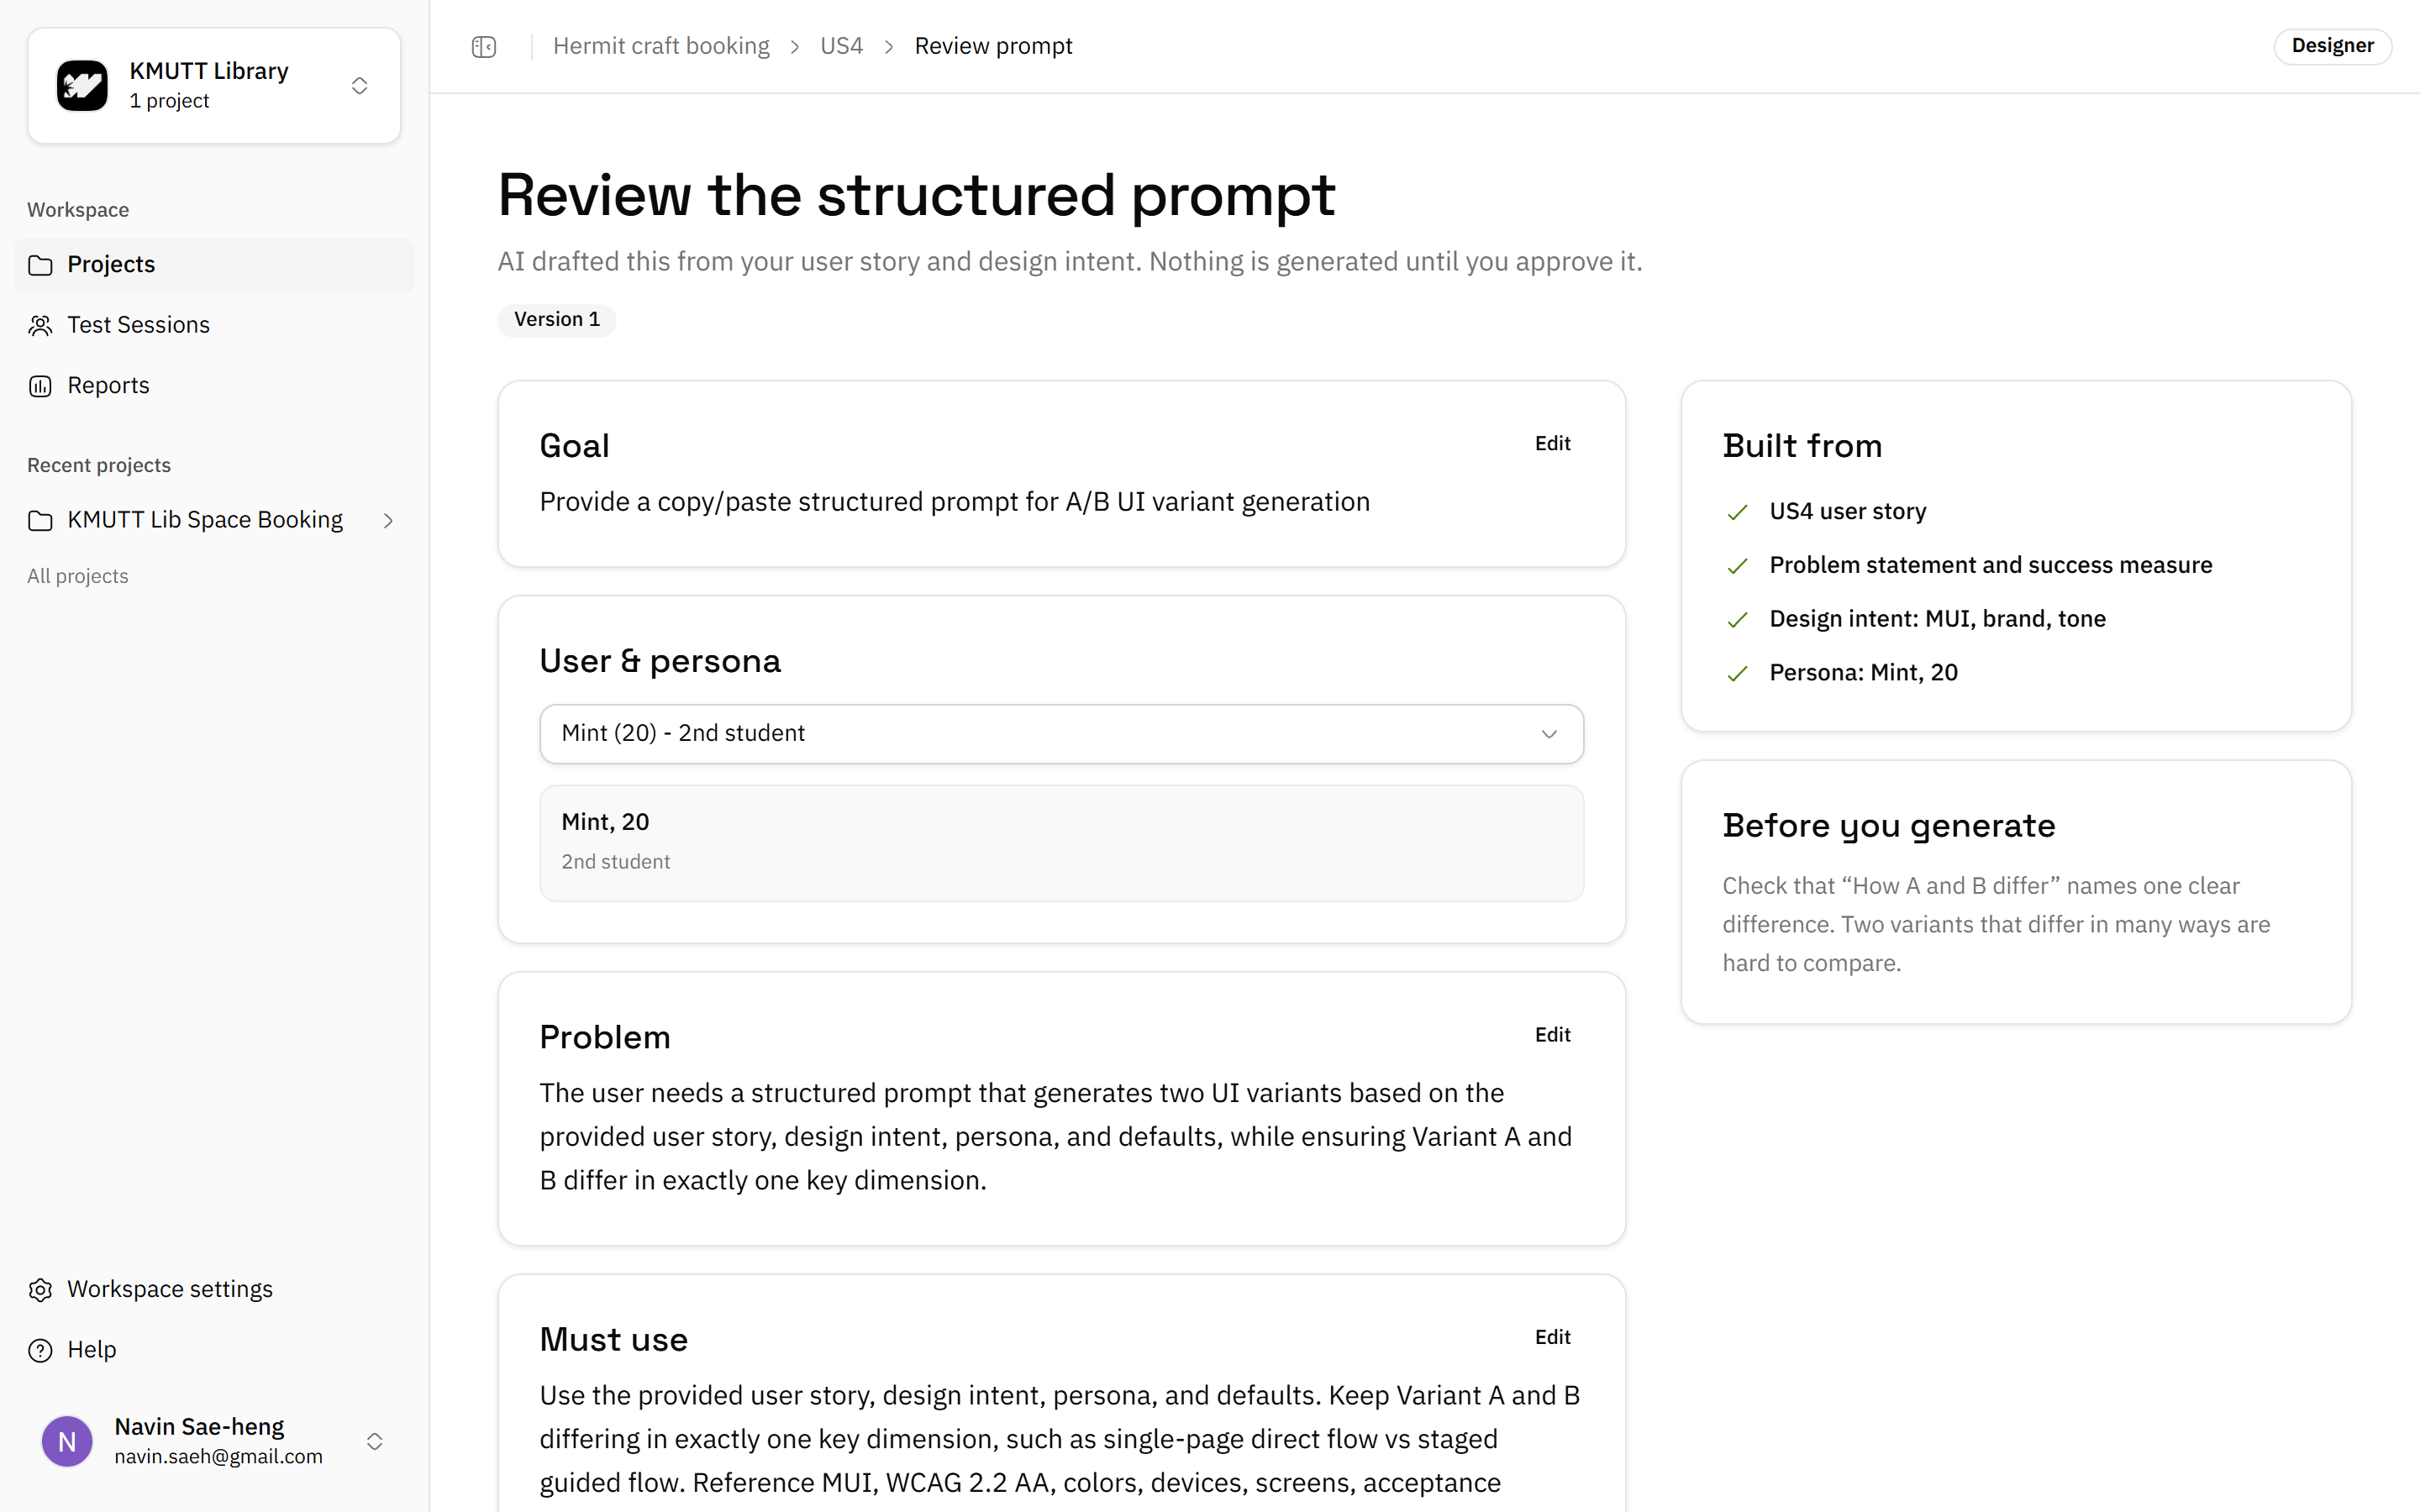
\includegraphics[width=0.9\linewidth]{figures/ch3-methodology/screens/prompt.png}
  \caption{หน้าจอตรวจ structured prompt ที่ AI ร่างก่อนสั่งสร้าง variant A และ B}
  \label{fig:screen-prompt}
\end{figure}
\thaijustify{
  จากนั้นระบบสร้าง UI variant ตามขั้นตอนในหัวข้อ~\ref{sec:ai-pipeline} ระหว่างนั้นหน้าจอแสดง generation trace แบบ real-time (รูปที่~\ref{fig:screen-generate-trace}) และนักออกแบบยกเลิกงานได้
}
\thaijustify{
  หลังได้ variant แล้ว นักออกแบบดูตัวอย่างหน้าจอและปรับแก้ผ่านแชต (chat-based refinement) การแก้แต่ละครั้งสร้าง variant เวอร์ชันใหม่ที่อ้างอิงฉบับเดิม จึงย้อนดูเวอร์ชันก่อนหน้าได้ เมื่อพอใจแล้วนักออกแบบอนุมัติ variant เพื่อนำไปทดสอบ สำหรับการกำหนดภารกิจและการเริ่มเซสชันการทดสอบ backend รองรับแล้ว แต่หน้าจอฝั่ง frontend อยู่ในแผนของภาคการศึกษาที่ 2
}
\begin{figure}[H]
  \centering
  \subfloat[Variant A: single-page direct flow]{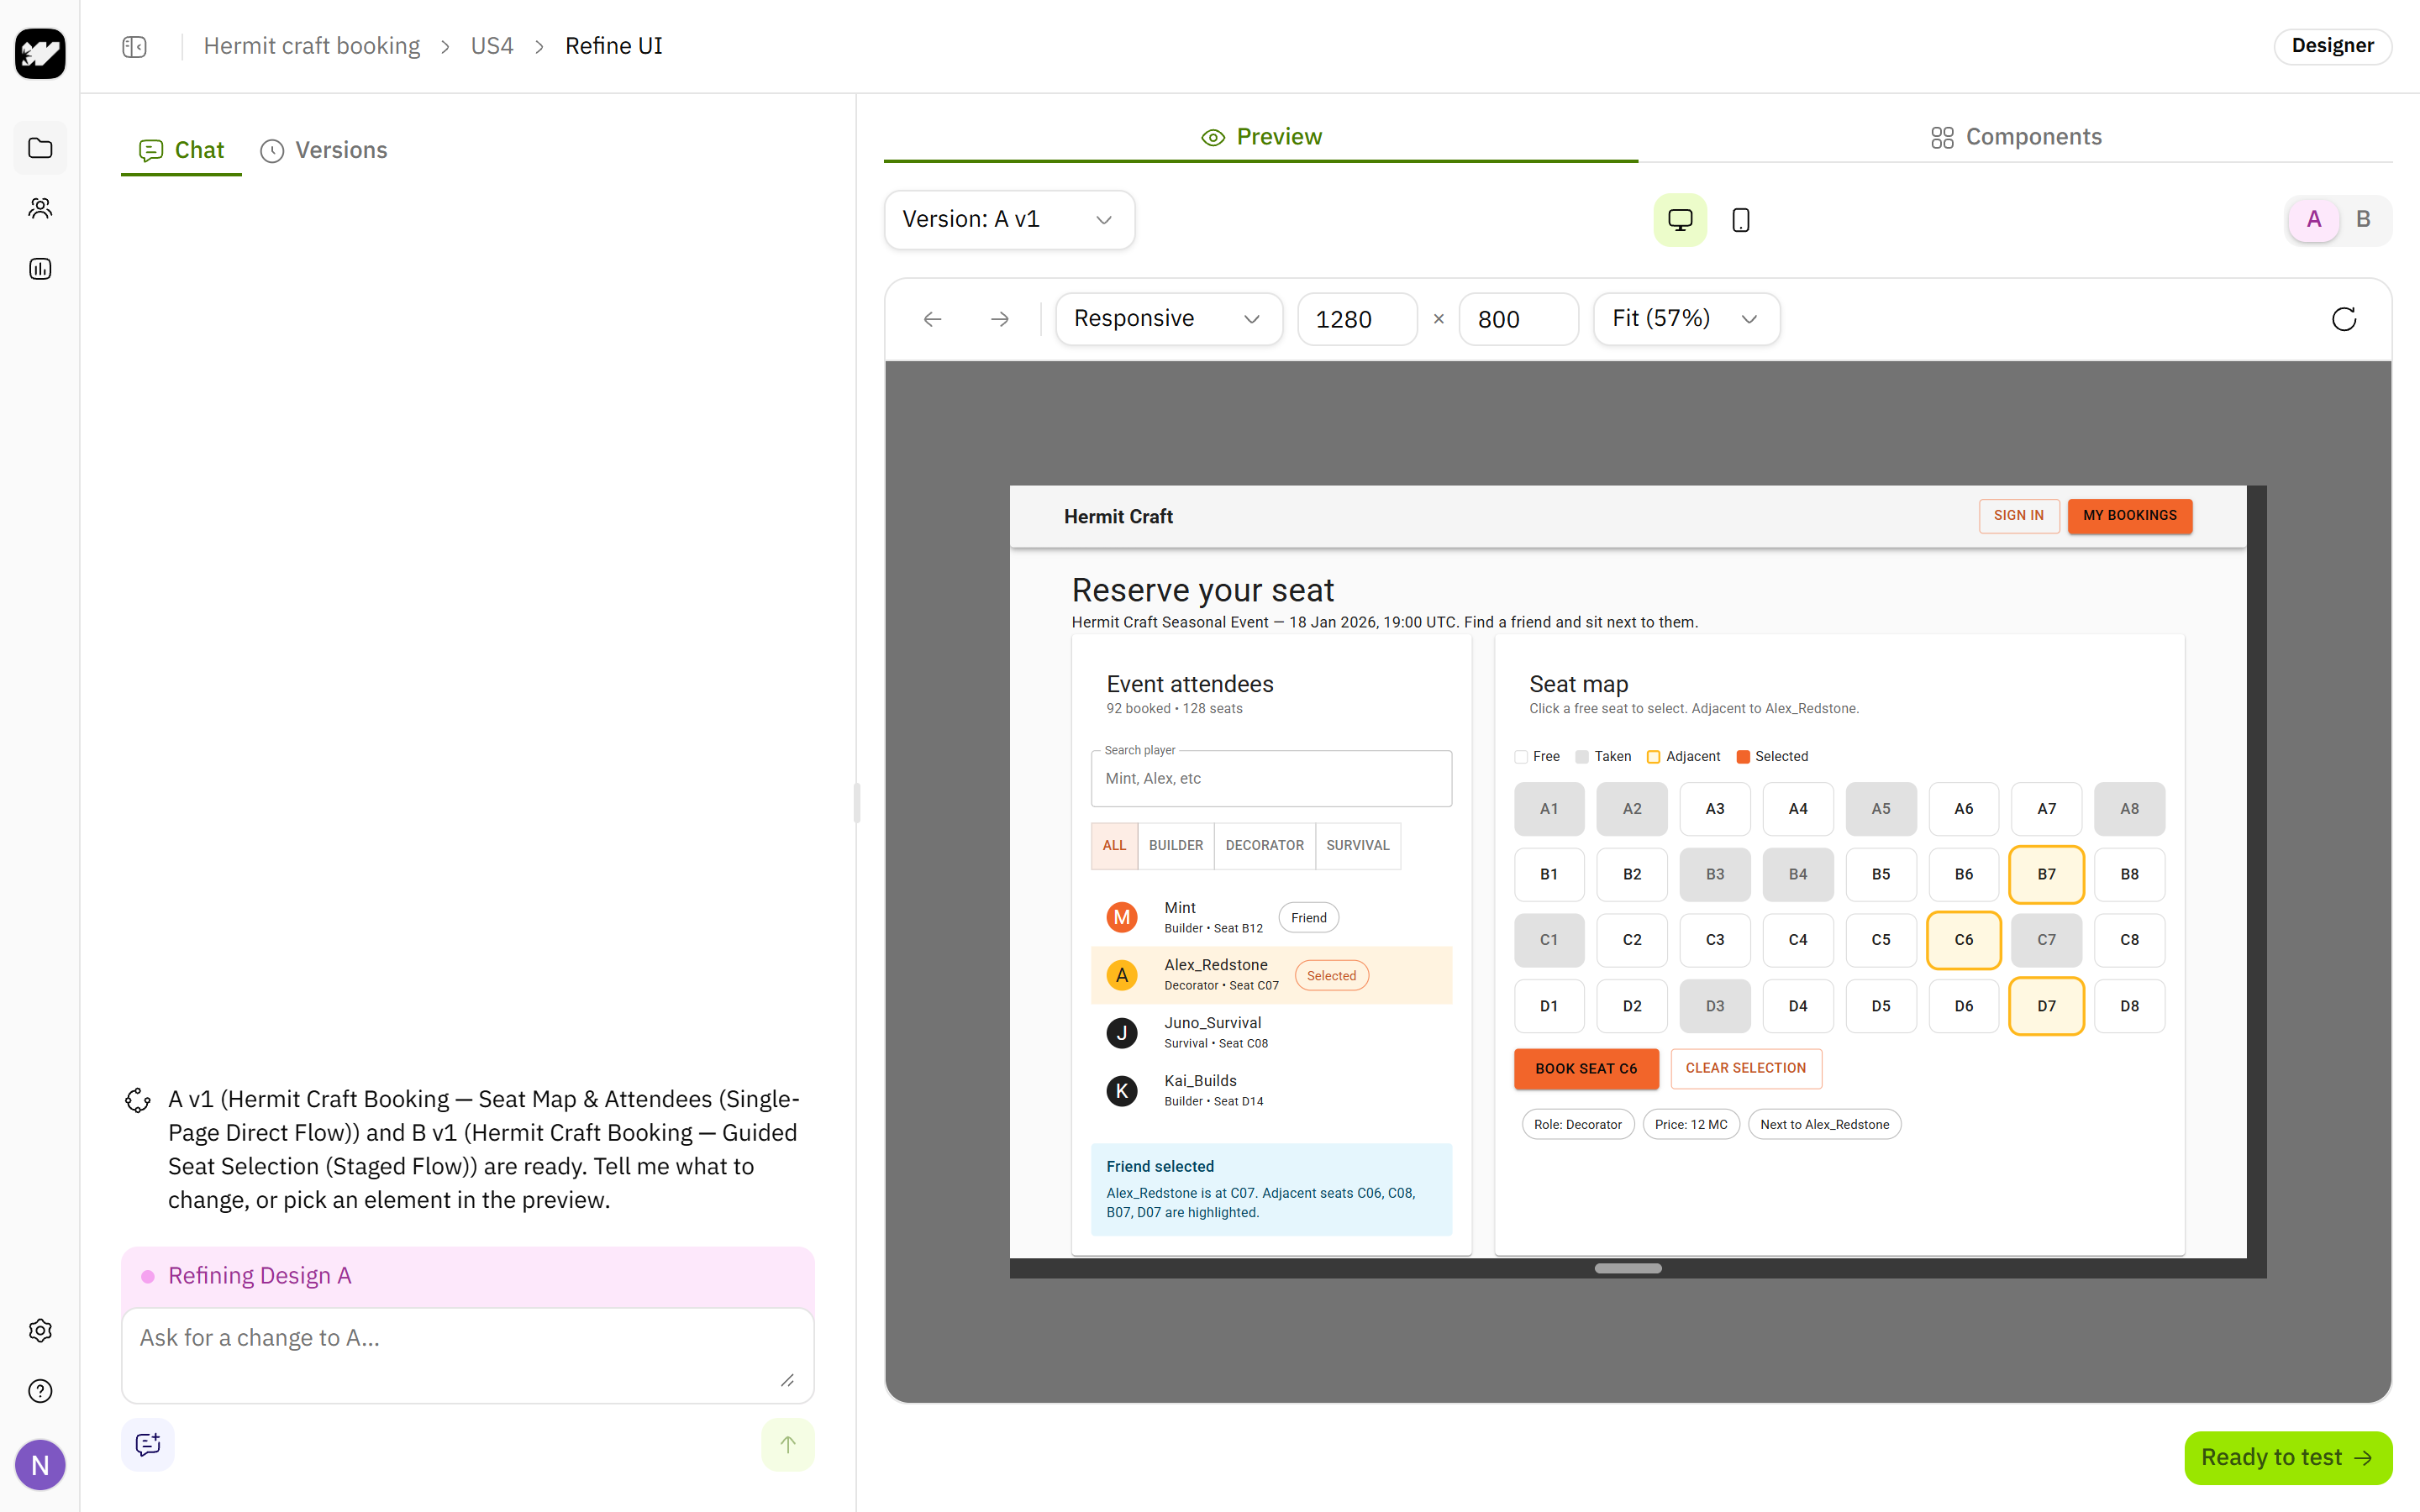
\includegraphics[width=0.49\linewidth]{figures/ch3-methodology/screens/refine-us4.png}}\hfill
  \subfloat[Variant B: staged guided flow]{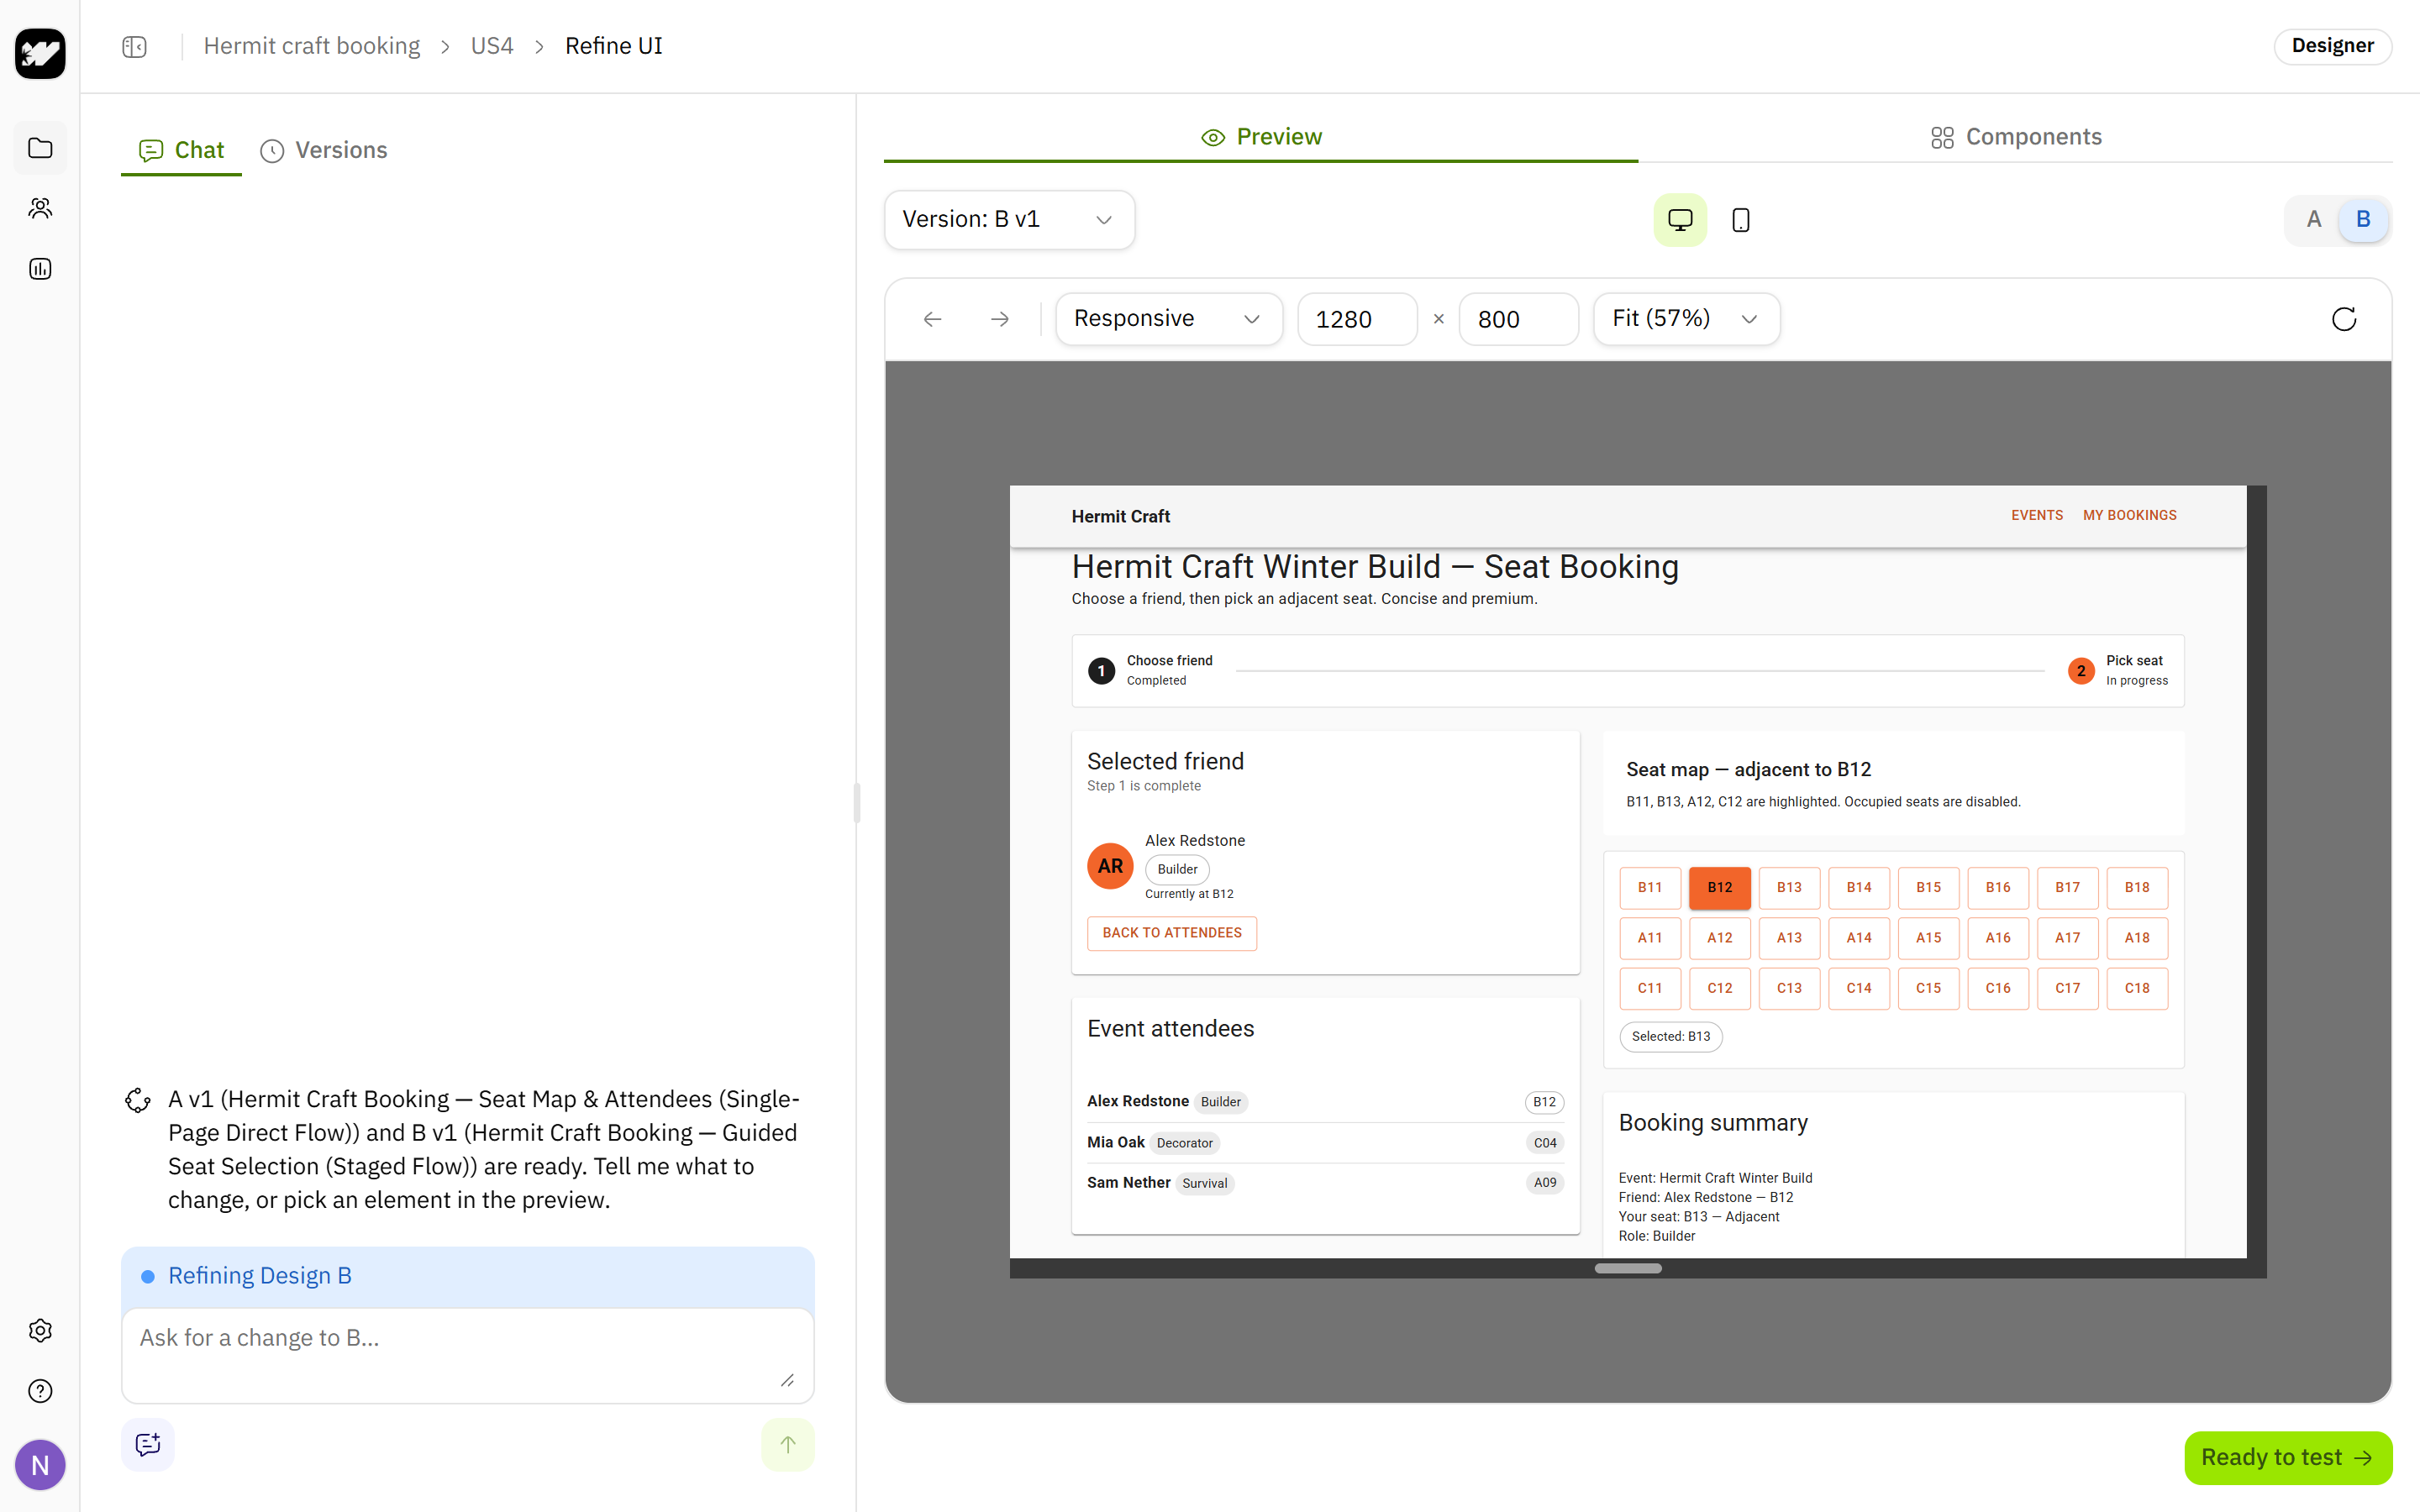
\includegraphics[width=0.49\linewidth]{figures/ch3-methodology/screens/refine-us4-b.png}}
  \caption{หน้าจอปรับแก้ variant ผ่านแชต (ซ้าย) พร้อมหน้าตัวอย่าง (ขวา) ของ two-alternative UI ที่ AI สร้างจาก user story เดียวกัน}
  \label{fig:screen-refine}
\end{figure}

\subsection{Application Program Interface}
\thaijustify{
  Backend ให้บริการผ่าน REST API ที่มีเอกสารแบบ OpenAPI ผ่าน Swagger UI API ส่วนใหญ่ต้องใช้ access token ของผู้ใช้ ส่วน API ของผู้เข้าร่วมทดสอบใช้ token ที่แลกได้จากลิงก์เชิญ ซึ่งมีอายุไม่เกินระยะเวลาของเซสชัน งานที่ใช้เวลานานมี endpoint แบบ SSE สำหรับติดตามความคืบหน้า กลุ่มของ API แสดงในตารางที่~\ref{tab:api-groups}
}
\begingroup
\small
\begin{xltabular}{\linewidth}{|>{\RaggedRight\arraybackslash}p{0.36\linewidth}|>{\RaggedRight\arraybackslash}X|}
  \caption{กลุ่มของ API ในระบบ}\label{tab:api-groups}\\
  \hline
  \textbf{Path} & \textbf{หน้าที่} \\ \hline
  \endfirsthead
  \hline
  \textbf{Path} & \textbf{หน้าที่} \\ \hline
  \endhead
  \texttt{/auth} & เข้าสู่ระบบด้วย Google, ขอ token ใหม่ และออกจากระบบ \\ \hline
  \texttt{/users} & ข้อมูลและรูปโปรไฟล์ของผู้ใช้ \\ \hline
  \texttt{/workspaces} & จัดการ workspace, สมาชิก, คำเชิญ และรูปประจำ workspace \\ \hline
  \texttt{/projects}, \texttt{/projects/:id/members} & จัดการโปรเจกต์และสมาชิกในโปรเจกต์ \\ \hline
  \texttt{/projects/:id/design-intent}, \texttt{personas}, \texttt{user-stories} & ความต้องการทางการออกแบบ, persona และ user story \\ \hline
  \texttt{/projects/:id/story-generations} & ให้ AI ร่าง user story (มี SSE) \\ \hline
  \texttt{/projects/:id/rounds} & รอบการออกแบบ, การร่าง prompt (SSE) และการอนุมัติรอบ \\ \hline
  \texttt{/projects/:id/rounds/:id/generation-jobs} & สั่ง ติดตาม (SSE) และยกเลิกงานสร้าง UI \\ \hline
  \texttt{/projects/:id/variants} & ดู ปรับแก้ อนุมัติ และดูประวัติเวอร์ชันของ variant \\ \hline
  \texttt{/projects/:id/test-sessions} & เซสชันการทดสอบ ภารกิจ ผู้เข้าร่วม และผลการทดสอบ \\ \hline
  \texttt{/testing} & API ของผู้เข้าร่วมทดสอบ: เข้าร่วม, ให้ความยินยอม, ทำภารกิจ, ส่งพฤติกรรมและข้อเสนอแนะ \\ \hline
  \texttt{/projects/:id/analyses}, \texttt{themes} & วิเคราะห์ข้อเสนอแนะด้วย AI และจัดการประเด็น \\ \hline
  \texttt{/projects/:id/rounds/:id/iterate}, \texttt{decisions} & เริ่มรอบถัดไปจากประเด็นที่เลือก และประวัติการตัดสินใจ \\ \hline
  \texttt{/projects/:id/shared-rounds}, \texttt{handoff}, \texttt{status}, \texttt{reports} & มุมมองและรายงานของ Client, Developer และ Project Manager \\ \hline
  \texttt{/projects/:id/audit-logs}, \texttt{/health} & บันทึกกิจกรรม และตรวจสถานะระบบ \\ \hline
\end{xltabular}
\endgroup
\thaijustify{
  API กลุ่มเซสชันการทดสอบ การวิเคราะห์ข้อเสนอแนะ และรายงาน พัฒนาส่วน backend ไว้ล่วงหน้าแล้ว ส่วนหน้าจอที่ใช้ API เหล่านี้อยู่ในแผนของภาคการศึกษาที่ 2
}
\begin{figure}[H]
  \centering
  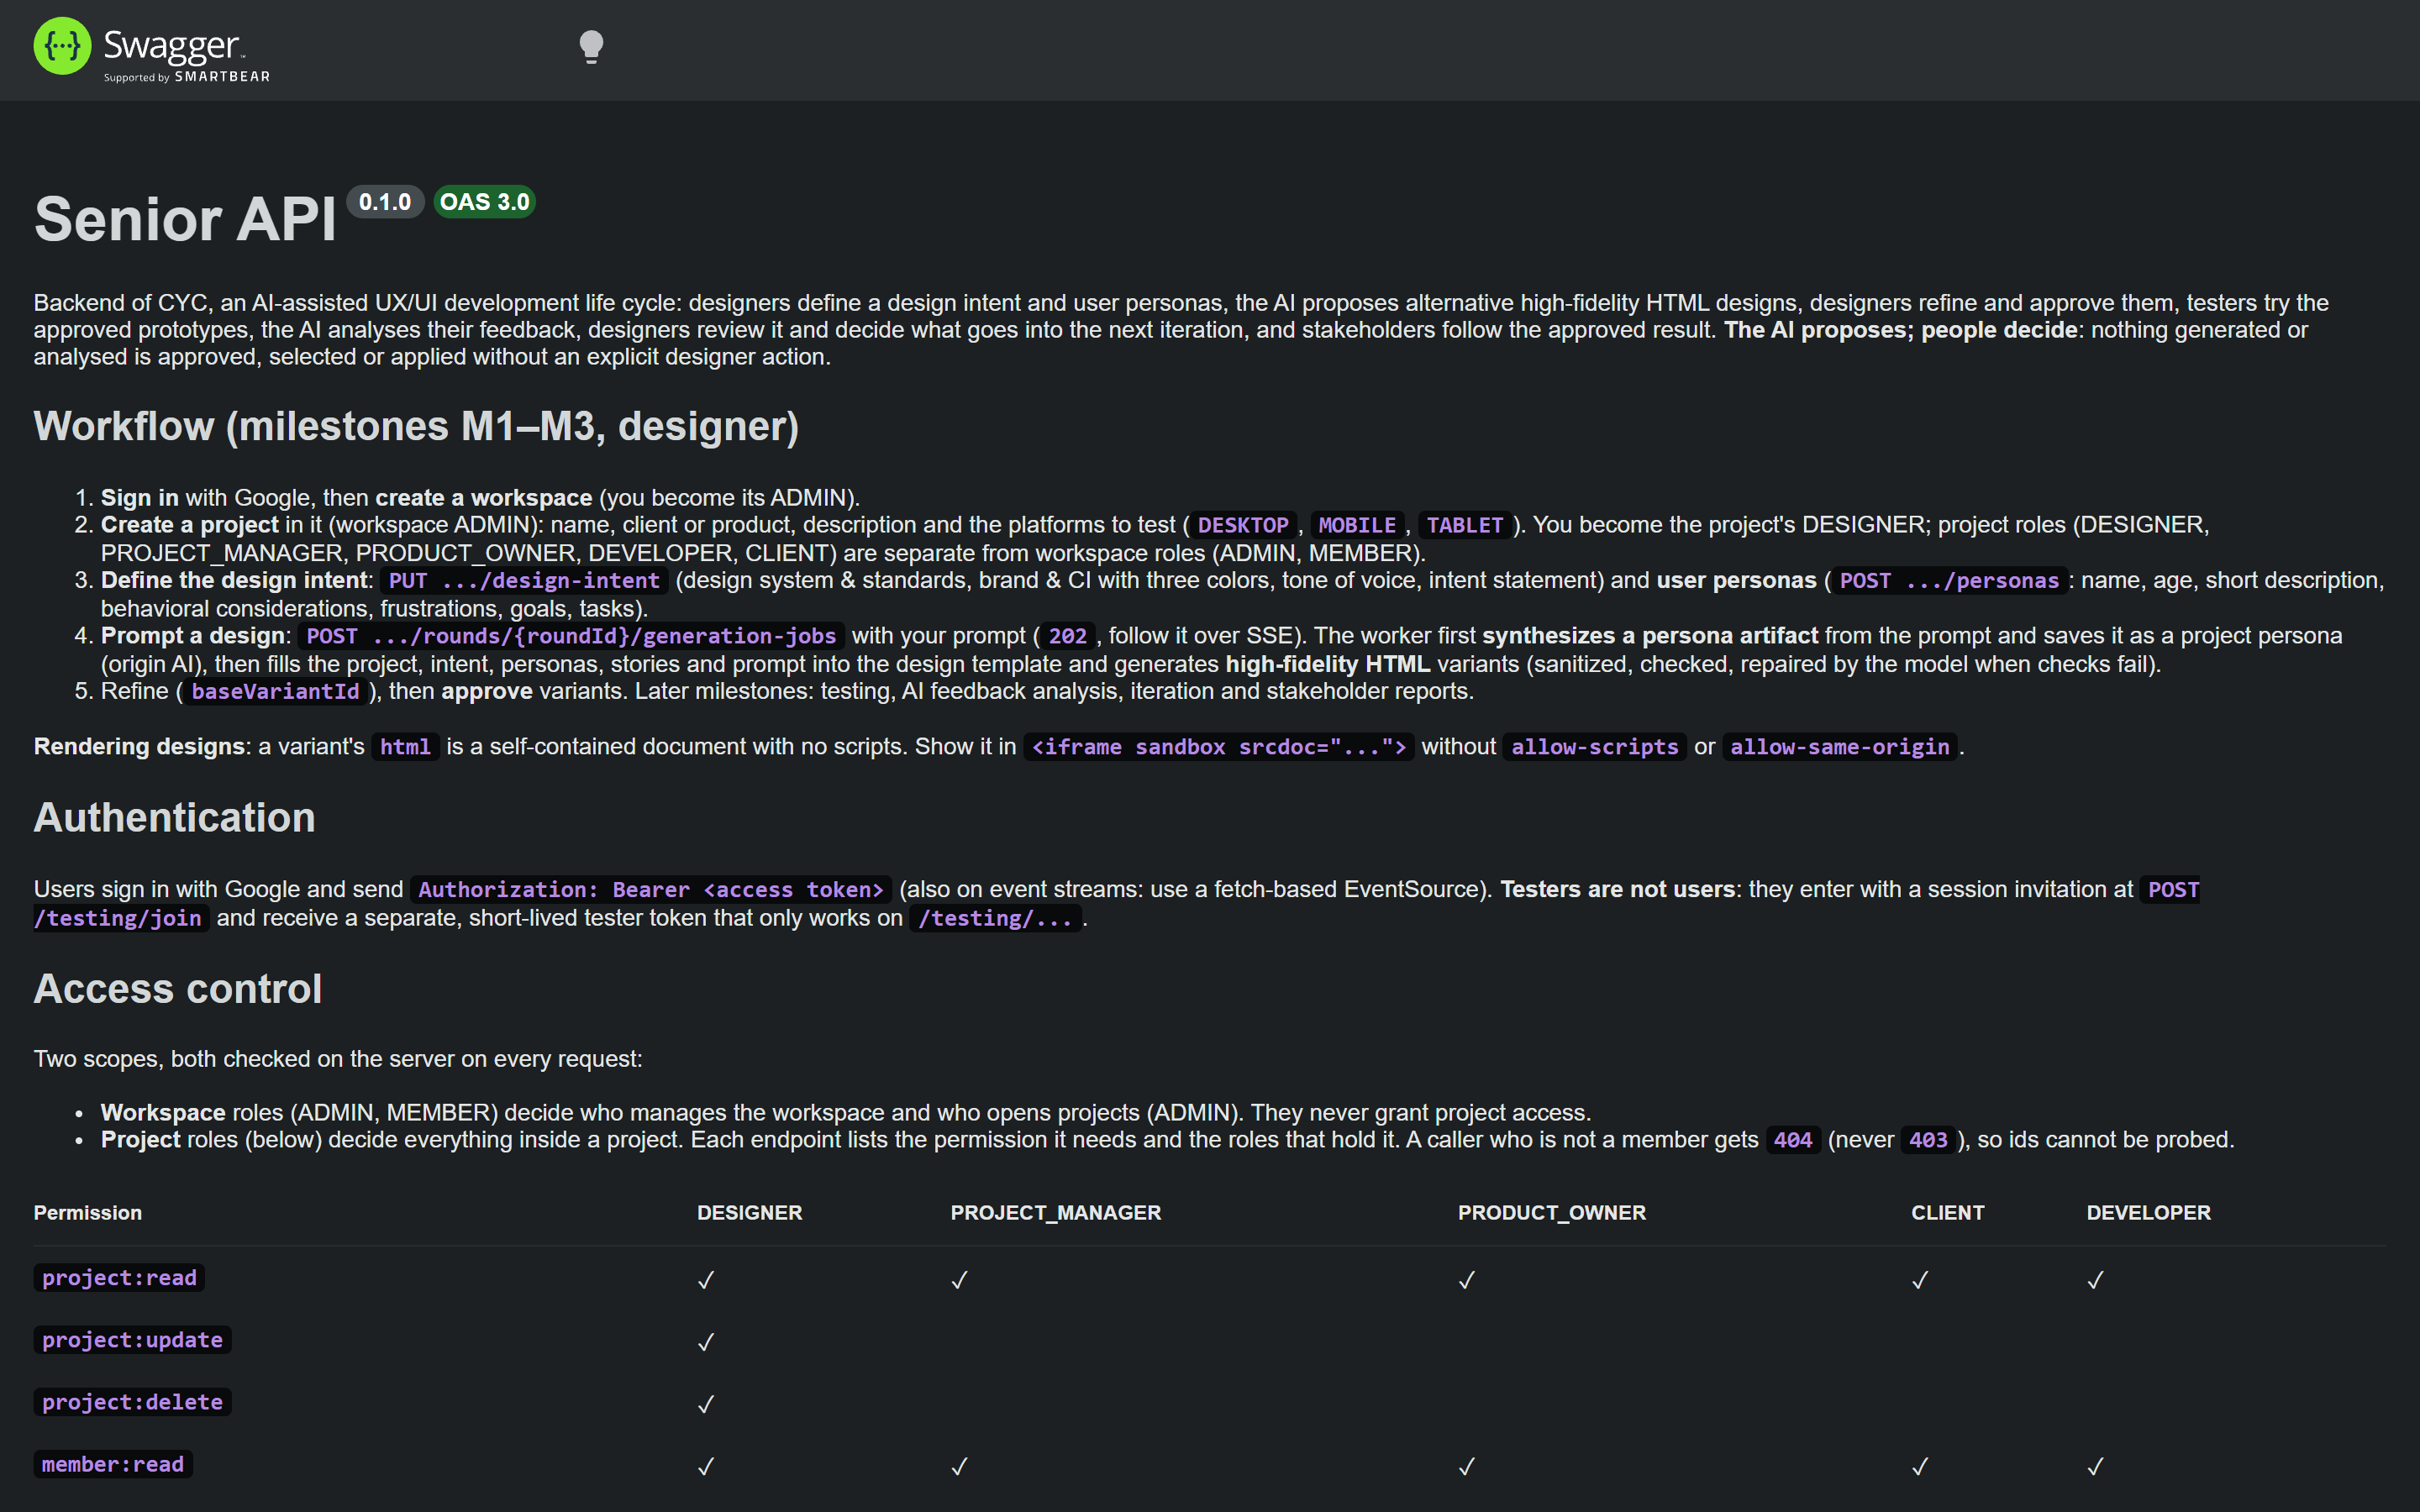
\includegraphics[width=0.9\linewidth]{figures/ch3-methodology/screens/swagger.png}
  \caption{เอกสาร API ผ่าน Swagger UI}
  \label{fig:screen-swagger}
\end{figure}

% !TeX root = ../../progress-sem1.tex
% Subsections of "การพัฒนาระบบ": developed screens per user group, matching
% "การพัฒนาหน้าจอเว็บไซต์ของ Admin / General User" in the example.
% Input from chapters/03-methodology.tex, after the API subsection.

\subsection{การพัฒนาหน้าจอเว็บไซต์ของ Designer}
\thaijustify{
  หน้าจอที่พัฒนาแล้วใน frontend เรียงตามลำดับการใช้งานของนักออกแบบ แสดงในตารางที่~\ref{tab:designer-screens}
}
\begingroup
\small
\begin{xltabular}{\linewidth}{|>{\RaggedRight\arraybackslash}p{0.40\linewidth}|>{\RaggedRight\arraybackslash}X|}
  \caption{หน้าจอของ Designer ที่พัฒนาแล้ว}\label{tab:designer-screens}\\
  \hline
  \textbf{Route} & \textbf{หน้าที่} \\ \hline
  \endfirsthead
  \hline
  \textbf{Route} & \textbf{หน้าที่} \\ \hline
  \endhead
  \texttt{/signin}, \texttt{/signup}, \texttt{/forgot-password} & เข้าสู่ระบบ สมัครสมาชิก และลืมรหัสผ่าน \\ \hline
  \texttt{/first-run}, \texttt{/workspaces/new} & การใช้งานครั้งแรกและการสร้าง workspace \\ \hline
  \texttt{/dashboard}, \texttt{/projects} & ภาพรวมและรายการโปรเจกต์แบบรายการและแกลเลอรี \\ \hline
  \texttt{/projects/new}, \texttt{.../setup/intent}, \texttt{.../setup/team} & wizard สร้างโปรเจกต์ กำหนด design intent และทีม \\ \hline
  \texttt{.../overview}, \texttt{.../intent}, \texttt{.../team} & ภาพรวมโปรเจกต์ แก้ไข design intent และสมาชิก \\ \hline
  \texttt{.../stories}, \texttt{.../stories/new}, \texttt{.../stories/:storyId} & จัดการ user story และ persona ของ story \\ \hline
  \texttt{.../stories/:storyId/prompt} & ตรวจและแก้ structured prompt ก่อนสร้าง UI \\ \hline
  \texttt{.../rounds/:roundId/generate} & สั่งสร้าง UI และดู generation trace \\ \hline
  \texttt{.../rounds/:roundId/refine} & ดูตัวอย่าง variant และปรับแก้ผ่านแชต \\ \hline
\end{xltabular}
\endgroup
\thaijustify{
  หน้า refine แบ่งเป็นแชตและหน้าตัวอย่างที่ปรับขนาดได้ นักออกแบบปักหมุดความคิดเห็นบนตำแหน่งใดก็ได้ของหน้าตัวอย่างแบบเดียวกับ Figma แล้วส่งหลายหมุดพร้อมกันเป็นคำสั่งปรับแก้ หมุดที่ส่งแล้วแสดงสถานะว่าถูกนำไปใช้ใน variant เวอร์ชันใด แถบด้านข้างย่อเป็น icon rail บนหน้านี้เพื่อเพิ่มพื้นที่แสดงผล
}
\thaijustify{
  ภาพหน้าจอของ wizard สร้างโปรเจกต์ design intent, user story, การตรวจ prompt และหน้า refine แสดงไว้ในหัวข้อ M2 และ M3 (รูปที่~\ref{fig:screen-project-new} ถึง~\ref{fig:screen-refine}) รูปที่~\ref{fig:screen-projects} และ~\ref{fig:screen-refine-pins} แสดงรายการโปรเจกต์และหมุดความคิดเห็นบนหน้า refine
}
\begin{figure}[H]
  \centering
  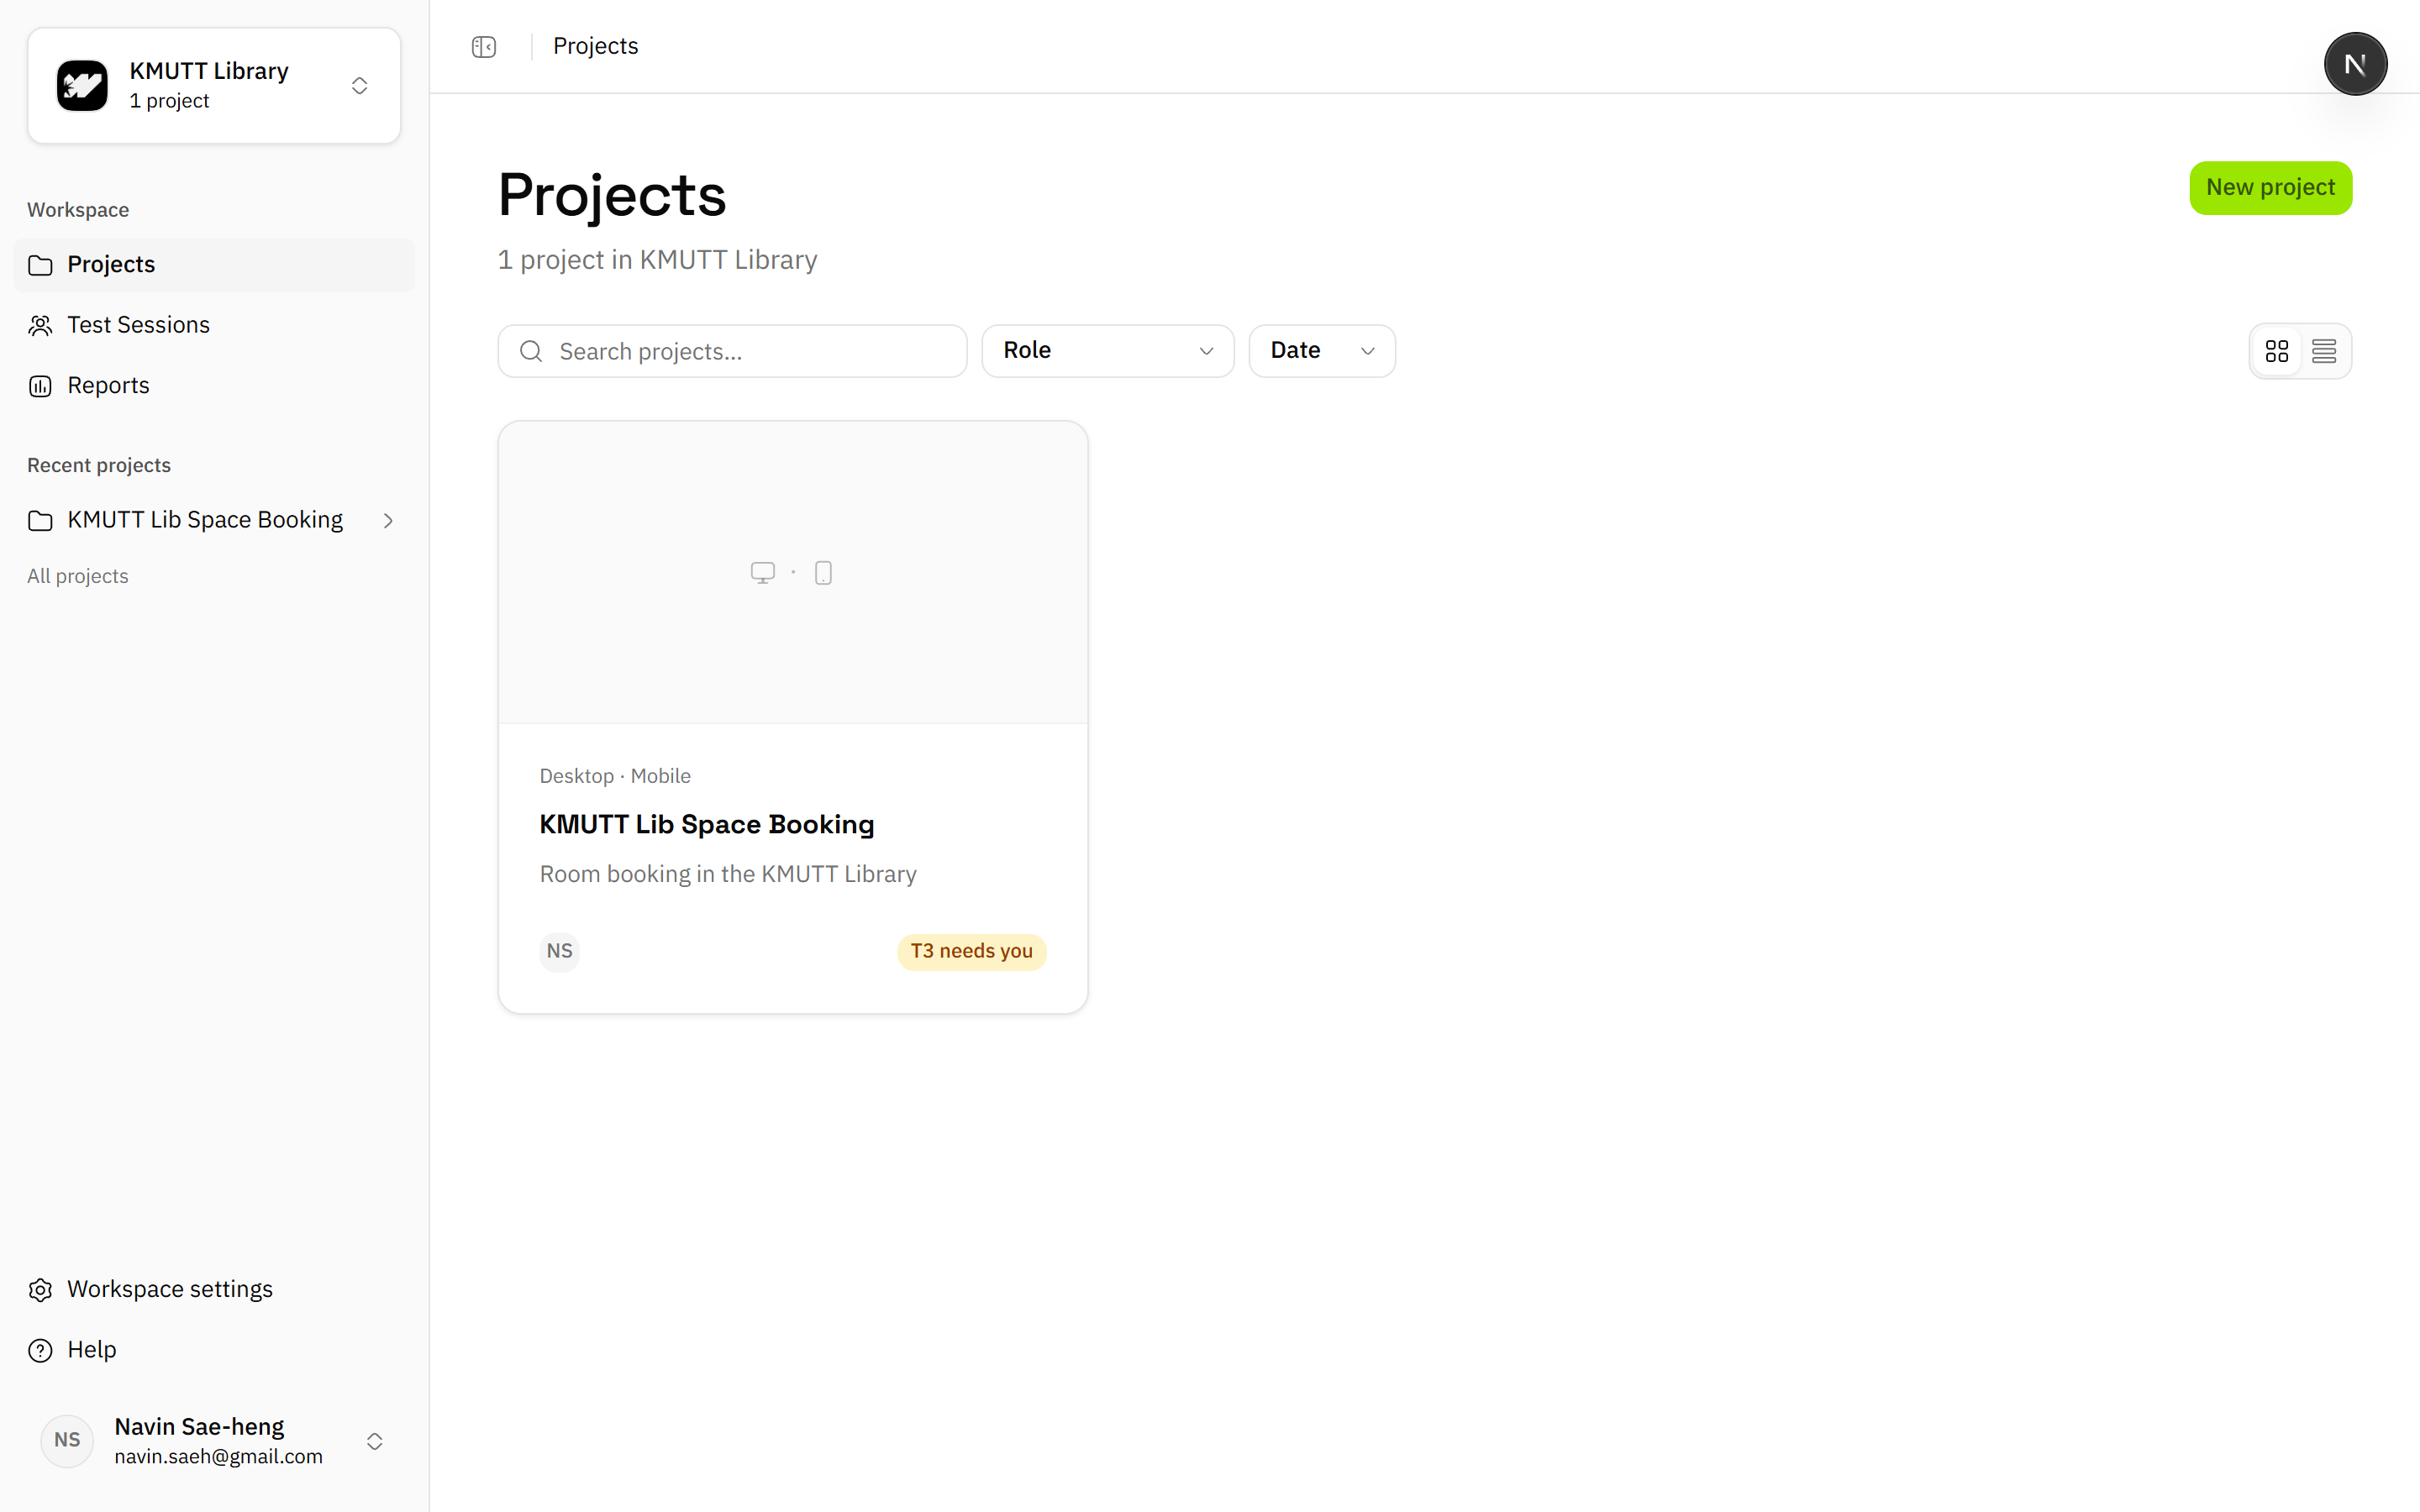
\includegraphics[width=0.9\linewidth]{figures/ch3-methodology/screens/projects.png}
  \caption{หน้ารายการโปรเจกต์ใน workspace}
  \label{fig:screen-projects}
\end{figure}
\begin{figure}[H]
  \centering
  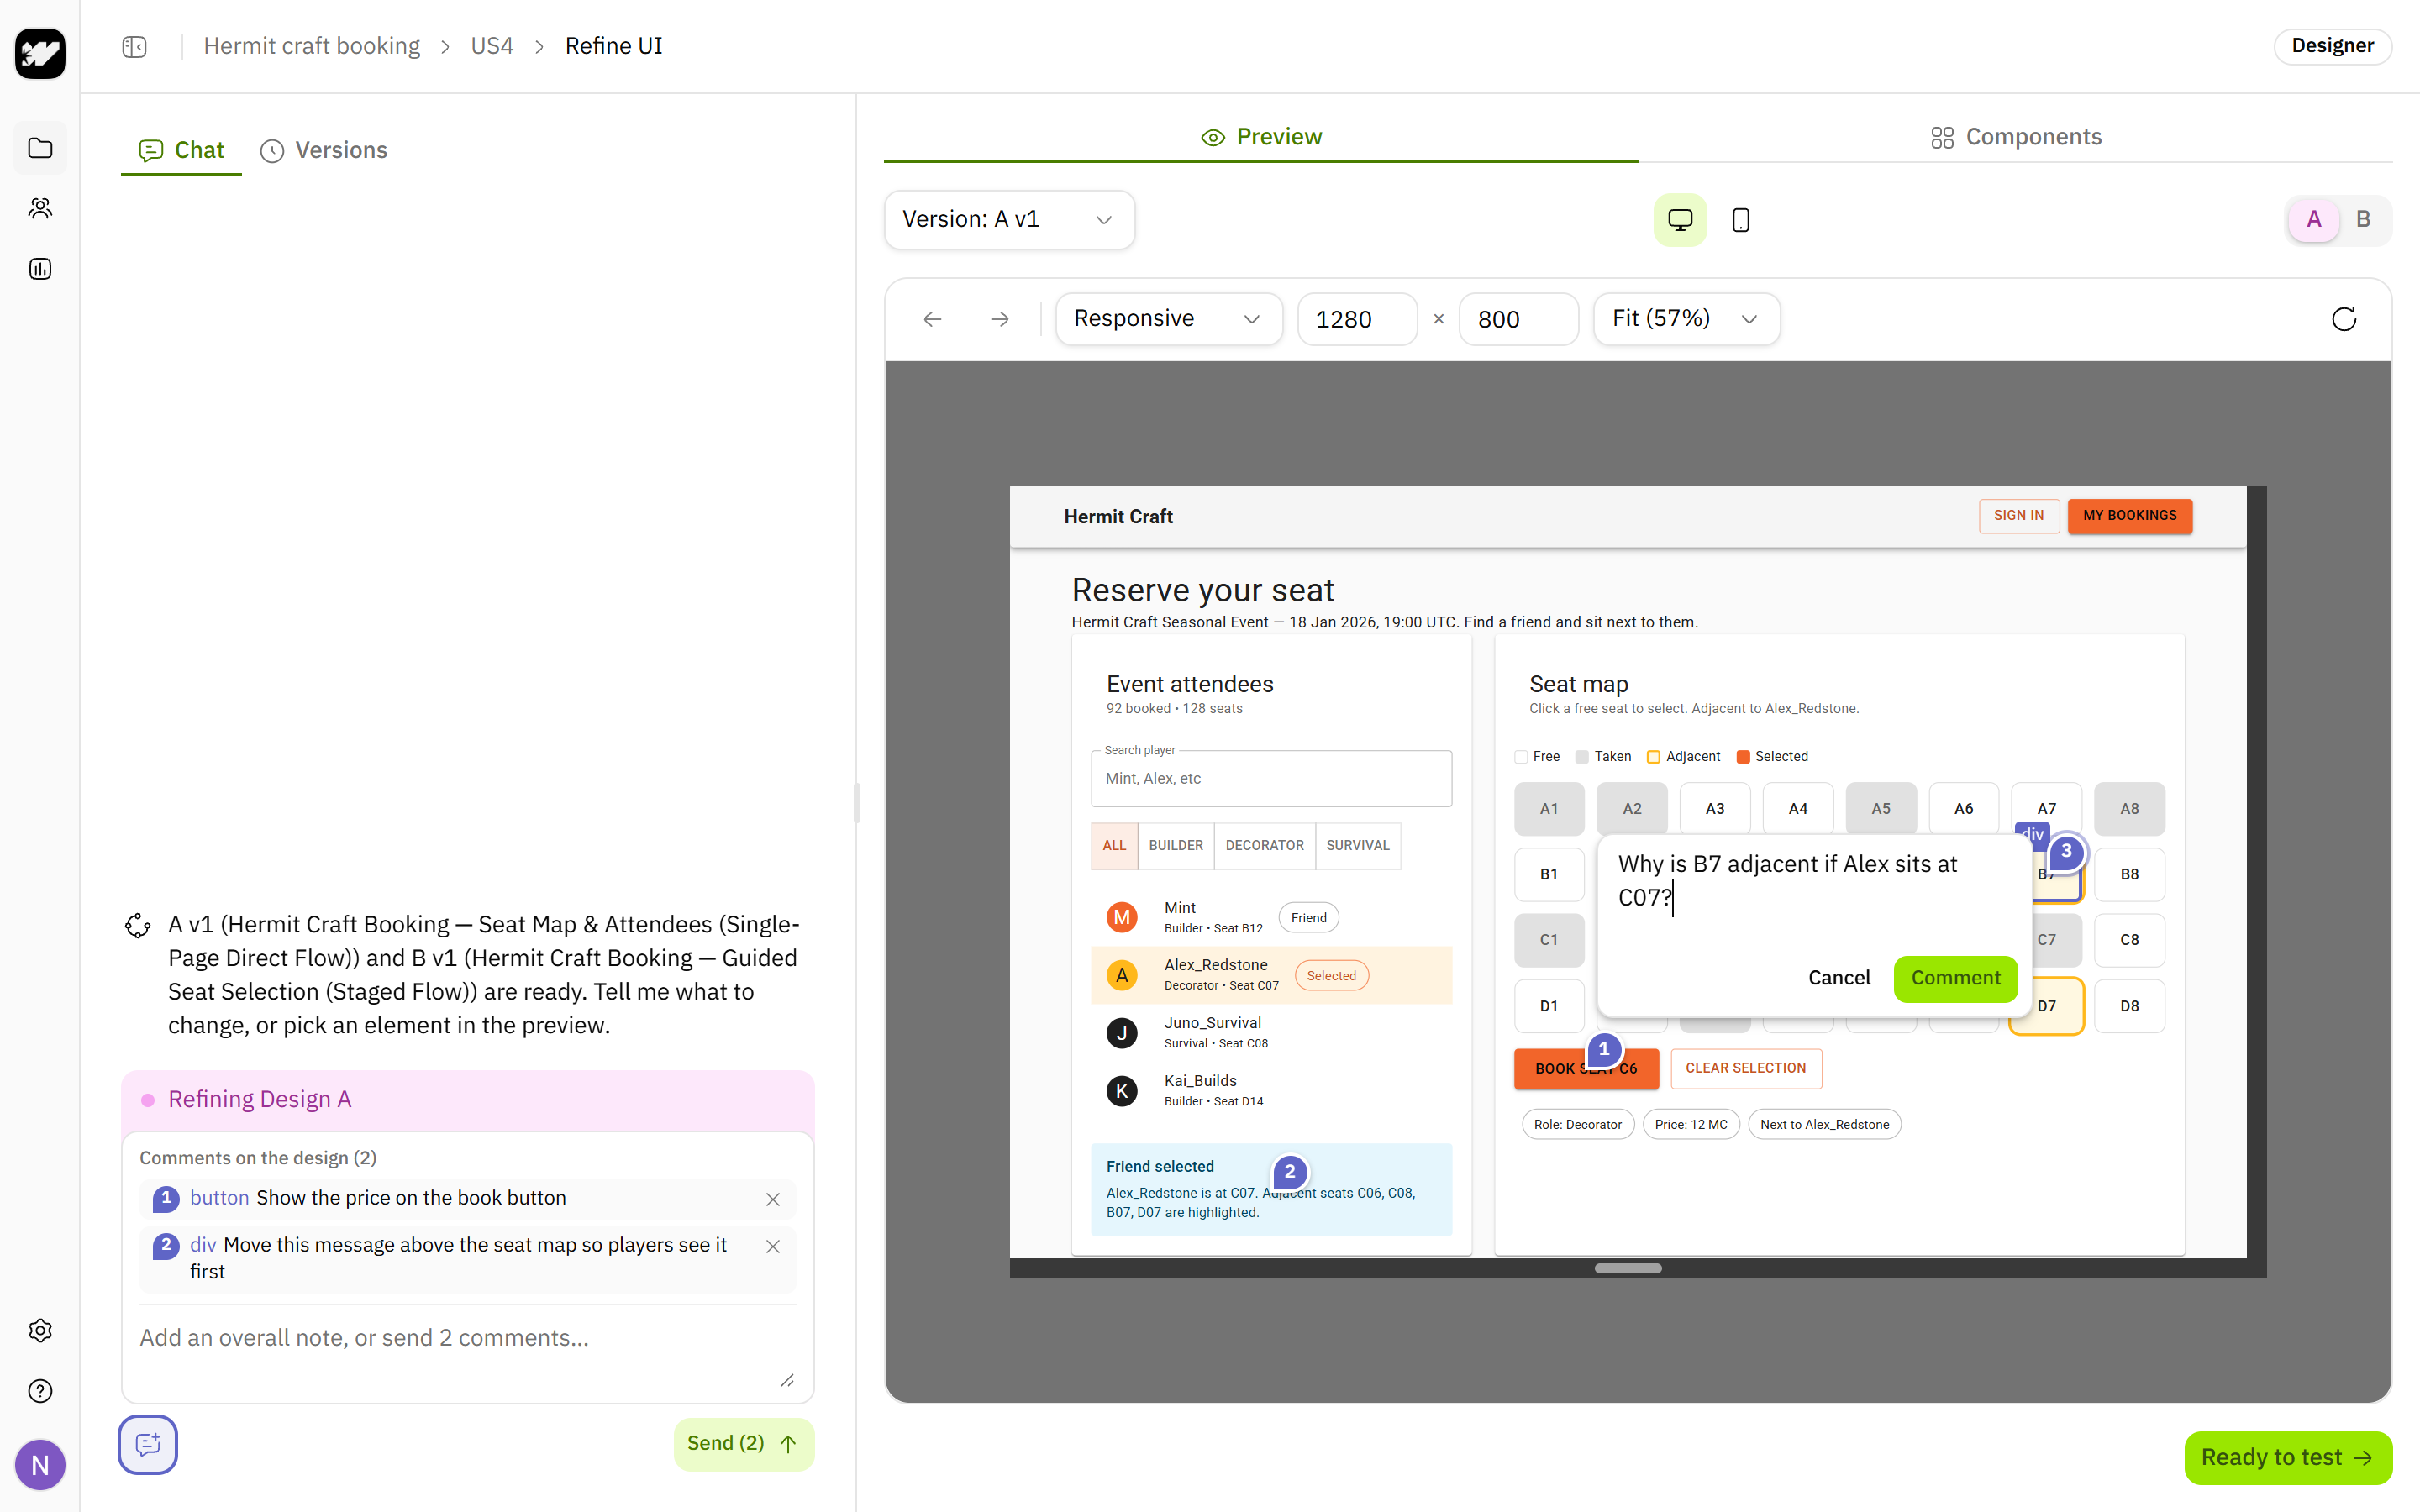
\includegraphics[width=0.9\linewidth]{figures/ch3-methodology/screens/refine-pins.png}
  \caption{หมุดความคิดเห็นบนหน้าตัวอย่างของ variant ในหน้า refine}
  \label{fig:screen-refine-pins}
\end{figure}

\subsection{การพัฒนาหน้าจอเว็บไซต์ของ Usability Tester และผู้มีส่วนได้ส่วนเสีย}
\thaijustify{
  หน้าจอเซสชันการทดสอบ (\texttt{.../sessions}) และรายงาน (\texttt{.../reports}) ปัจจุบันเป็นแท็บในหน้าโปรเจกต์ที่รอเชื่อมกับ API ซึ่ง backend พัฒนาไว้แล้ว (ตารางที่~\ref{tab:api-groups}) หน้าจอของผู้เข้าร่วมทดสอบ และมุมมองของ Client, Developer และ Project Manager อยู่ในแผนของภาคการศึกษาที่ 2
}



%%%%%%%%%%%%%%%%%%%%%%%%%%%%%%%%% Chapter 4 %%%%%%%%%%%%%%%%%%%%%%%%%%%%%
\chapter{ผลการดำเนินงาน}
% !TeX root = ../../../progress-sem1.tex
% Progress sem 1, chapter 4 opening paragraph
\thaijustify{
  ในบทที่ 4 จะกล่าวถึงผลการดำเนินงานในภาคการศึกษาที่ 1 เทียบกับแผนที่วางไว้ การประเมินผลการดำเนินงาน ปัญหาและอุปสรรคที่พบ และแผนการดำเนินงานในภาคการศึกษาที่ 2
}

% !TeX root = ../../../progress-sem1.tex
% 4.x สรุปผลการดำเนินงานเทียบกับแผน (semester 1)
\section{สรุปผลการดำเนินงานเทียบกับแผน}
\thaijustify{
  ตารางที่~\ref{tab:progress-status} สรุปสถานะของงานใน milestone M0 ถึง M3 ซึ่งเป็นแผนของภาคการศึกษาที่ 1 ณ วันที่ 26 พฤศจิกายน 2569 โดยพิจารณาจากซอร์สโค้ดใน branch หลักของ repository
}
\begingroup
\small
\begin{xltabular}{\linewidth}{|>{\RaggedRight\arraybackslash}X|>{\RaggedRight\arraybackslash}p{0.15\linewidth}|>{\RaggedRight\arraybackslash}p{0.36\linewidth}|}
  \caption{สถานะของงานในภาคการศึกษาที่ 1}\label{tab:progress-status}\\
  \hline
  \textbf{งาน} & \textbf{สถานะ} & \textbf{หมายเหตุ} \\ \hline
  \endfirsthead
  \multicolumn{3}{l}{\textit{ตารางที่ \thetable\ (ต่อ)}}\\
  \hline
  \textbf{งาน} & \textbf{สถานะ} & \textbf{หมายเหตุ} \\ \hline
  \endhead
  \multicolumn{3}{|l|}{\textbf{M0: Foundation}} \\ \hline
  ระบุกลุ่มเป้าหมาย ขอบเขต และ MVP & แล้วเสร็จ & บทที่ 1 \\ \hline
  กำหนด data model & แล้วเสร็จ & 34 ตาราง ครอบคลุมทุก milestone (หัวข้อ~\ref{sec:er-diagram}) \\ \hline
  เลือก architecture: auth, LLM provider, prototype rendering, hosting & ดำเนินการบางส่วน & เลือกแล้วทุกส่วนยกเว้นบริการที่ใช้ deploy \\ \hline
  สำรวจและเลือก design system และ UI kit & แล้วเสร็จ & shadcn/ui สำหรับแพลตฟอร์ม และ UI kit shadcn/ui กับ MUI สำหรับ AI \\ \hline
  กำหนด requirements ด้าน PDPA และข้อความขอ consent & แล้วเสร็จ & เก็บความยินยอมพร้อมเวอร์ชันของข้อความ \\ \hline
  ตั้งค่า CI/CD, environments และ event analytics & ดำเนินการบางส่วน & มี CI และสภาพแวดล้อมสำหรับพัฒนาแล้ว ยังไม่มี CD และ event analytics \\ \hline
  การกำหนดดัชนีชี้วัดผล และแผนการดำเนินงาน & แล้วเสร็จ &  \\ \hline
  \multicolumn{3}{|l|}{\textbf{M1: Secure Access}} \\ \hline
  จัดทำ Landing page & แล้วเสร็จ &  \\ \hline
  จัดทำ Register page & ดำเนินการบางส่วน & หน้าจอเสร็จแล้ว backend อยู่ใน branch แยก \\ \hline
  การยืนยันตัวตนผ่านอีเมล & ดำเนินการบางส่วน & อยู่ระหว่างพัฒนาใน branch แยก \\ \hline
  การเข้าสู่ระบบพร้อมระบบจัดการข้อผิดพลาด & ดำเนินการบางส่วน & เข้าสู่ระบบด้วย Google ได้แล้ว อีเมลและรหัสผ่านอยู่ใน branch แยก \\ \hline
  ระบบรีเซ็ตรหัสผ่าน & ดำเนินการบางส่วน & หน้าจอเสร็จแล้ว backend อยู่ใน branch แยก \\ \hline
  ระบบควบคุมการเข้าถึง & แล้วเสร็จ & ควบคุมสิทธิ์ตาม permission ของแต่ละบทบาท \\ \hline
  จัดทำระบบ routing ตามบทบาทของผู้ใช้ & ดำเนินการบางส่วน & backend ตรวจสิทธิ์ตามบทบาทแล้ว หน้าจอของ Client, Developer และ PM อยู่ใน M6 \\ \hline
  ทดสอบระบบยืนยันตัวตนและการควบคุมการเข้าถึง & ดำเนินการบางส่วน & มี unit test และ end-to-end test ของ auth และสิทธิ์ ยังขาดส่วนอีเมลและรหัสผ่าน \\ \hline
  \multicolumn{3}{|l|}{\textbf{M2: Project Setup}} \\ \hline
  ระบบสร้าง workspace & แล้วเสร็จ & รวมการเชิญสมาชิกและรูปประจำ workspace \\ \hline
  ระบบสร้างโปรเจกต์ & แล้วเสร็จ & รวมการกำหนดสมาชิกและบทบาทในโปรเจกต์ \\ \hline
  ฟอร์มกำหนดความต้องการทางการออกแบบ & แล้วเสร็จ &  \\ \hline
  ระบบจัดเก็บความต้องการทางการออกแบบเพื่อใช้เป็น reusable AI context & แล้วเสร็จ & เก็บเวอร์ชันของ design intent ที่ใช้ในแต่ละงาน \\ \hline
  \multicolumn{3}{|l|}{\textbf{M3: AI Design Generation}} \\ \hline
  การสร้าง User story และ Problem statement & แล้วเสร็จ & การให้ AI ร่าง user story มีเฉพาะ backend \\ \hline
  เครื่องมือสร้างคำสั่งที่รวมความต้องการทางการออกแบบและ user story & แล้วเสร็จ &  \\ \hline
  การสร้าง two-alternative UI & แล้วเสร็จ & มีการตรวจและให้โมเดลแก้ไขอัตโนมัติ \\ \hline
  การปรับปรุง UI (Chat-based) & แล้วเสร็จ & เก็บประวัติแต่ละเวอร์ชัน \\ \hline
  การดูตัวอย่างรูปแบบหน้าจอ & แล้วเสร็จ &  \\ \hline
  การอนุมัติและมอบหมายงานให้ผู้เข้าร่วมทดสอบ & ดำเนินการบางส่วน & อนุมัติ variant ได้แล้ว การมอบหมายงานมีเฉพาะ backend \\ \hline
  การเริ่มเซสชันการทดสอบ & ดำเนินการบางส่วน & backend สร้างลิงก์และรหัสได้แล้ว หน้าจอยังไม่มี \\ \hline
  ชุดข้อมูลสำหรับการประเมินคุณภาพผลลัพธ์ของ AI & ยังไม่เริ่ม &  \\ \hline
\end{xltabular}
\endgroup
\thaijustify{
  นอกจากงานตามแผนแล้ว ทีมได้พัฒนาส่วน backend ของ M4 ถึง M6 ไว้ล่วงหน้า ได้แก่ เซสชันการทดสอบพร้อมการเก็บความยินยอม การบันทึกภารกิจ พฤติกรรม และข้อเสนอแนะของผู้เข้าร่วมทดสอบ การวิเคราะห์ข้อเสนอแนะด้วย AI การจัดการประเด็นและบันทึกการตัดสินใจ รวมถึงมุมมองและรายงานสำหรับผู้มีส่วนได้ส่วนเสีย ส่วนหน้าจอของงานเหล่านี้อยู่ในแผนของภาคการศึกษาที่ 2
}

% !TeX root = ../../../progress-sem1.tex
% 4.x การประเมินผลการดำเนินงาน (semester 1)
% Counts from cyc-monorepo main at commit 5ce62d1 (25 Nov 2026) and tab:progress-status.
\section{การประเมินผลการดำเนินงาน}
\subsection{ความคืบหน้าเทียบกับแผน}
\thaijustify{
  จากงาน 27 รายการใน milestone M0 ถึง M3 (ตารางที่~\ref{tab:progress-status}) งานที่แล้วเสร็จมี 16 รายการ ดำเนินการบางส่วน 10 รายการ และยังไม่เริ่ม 1 รายการ M2 แล้วเสร็จครบทุกรายการ และ M3 ซึ่งเป็นส่วนหลักของภาคการศึกษานี้ใช้งานได้ตั้งแต่การเขียน user story จนถึงการปรับแก้ UI ผ่านแชต งานที่ยังค้างส่วนใหญ่อยู่ใน M1 คือการสมัครสมาชิกด้วยอีเมลและรหัสผ่าน ซึ่งอยู่ระหว่างพัฒนาใน branch แยก และงานที่ต่อเนื่องไปยังการทดสอบ ได้แก่ การมอบหมายงานให้ผู้เข้าร่วมทดสอบและการเริ่มเซสชัน ซึ่งพัฒนาเฉพาะ backend ไว้แล้ว ส่วนงานที่ยังไม่เริ่มคือชุดข้อมูลสำหรับประเมินคุณภาพผลลัพธ์ของ AI
}
\subsection{งานที่ทำได้ล่วงหน้า}
\thaijustify{
  ทีมพัฒนา backend ของ M4 ถึง M6 ไว้ก่อนแผน และออกแบบหน้าจอ high-fidelity ครบทุกกลุ่มผู้ใช้แล้ว รวมถึงหน้าจอของผู้เข้าร่วมทดสอบและผู้มีส่วนได้ส่วนเสียที่จะพัฒนาในภาคการศึกษาที่ 2 (หัวข้อ~\ref{sec:ui-prototype}) จึงเริ่มพัฒนาหน้าจอของภาคการศึกษาที่ 2 ได้ทันทีโดยไม่ต้องรอการออกแบบ
}
\subsection{คุณภาพของซอฟต์แวร์}
\thaijustify{
  ณ commit 5ce62d1 (25 พฤศจิกายน 2569) ใน branch หลัก backend มีไฟล์ unit test 24 ไฟล์ และ end-to-end test 4 ไฟล์ ครอบคลุมการยืนยันตัวตน การควบคุมสิทธิ์ cache และการสร้าง UI การเปลี่ยนแปลงทั้งหมดผ่าน pull request ซึ่ง merge แล้ว 16 ครั้ง และทุก pull request ผ่านการตรวจ lint และ build อัตโนมัติก่อน merge
}
\subsection{คุณภาพผลลัพธ์ของ AI}
\thaijustify{
  ในภาคการศึกษานี้ระบบควบคุมคุณภาพของ UI ที่ AI สร้างด้วยการตรวจอัตโนมัติก่อนแสดงผล ได้แก่ การใช้ component ของ UI kit สีแบรนด์ platform และมาตรฐานการเข้าถึง ร่วมกับการให้โมเดลแก้ไขเมื่อไม่ผ่าน (หัวข้อ~\ref{sec:ai-pipeline}) แต่ยังไม่ได้ประเมินคุณภาพของผลลัพธ์เชิงปริมาณ เช่น สัดส่วนของ variant ที่ผ่านการตรวจในครั้งแรก หรือการให้คะแนนโดยนักออกแบบ ซึ่งจะทำพร้อมกับการจัดทำชุดข้อมูลประเมินในภาคการศึกษาที่ 2
}

% !TeX root = ../../../progress-sem1.tex
% 4.x ปัญหาและอุปสรรคที่พบ (semester 1)
\section{ปัญหาและอุปสรรคที่พบ}
\subsection{ปัญหาและแนวทางแก้ไข}
\thaijustify{
  \begin{enumerate}
    \item \textbf{ผลลัพธ์ของ AI ไม่สม่ำเสมอ}\\
      UI ที่โมเดลสร้างในบางครั้งใช้ component ที่ไม่อยู่ใน UI kit ใช้สีไม่ตรงกับแบรนด์ หรือไม่ผ่านมาตรฐานการเข้าถึง ทีมแก้ไขโดยเพิ่มขั้นตรวจอัตโนมัติหลังสร้างทุกครั้ง หากไม่ผ่าน ระบบส่งปัญหาที่พบกลับให้โมเดลแก้ได้สูงสุดสองครั้ง และหากยังไม่ผ่านจะเริ่มสร้าง variant นั้นใหม่อีกหนึ่งครั้ง
    \item \textbf{การสร้าง UI ใช้เวลานาน}\\
      การสร้าง variant แต่ละชุดใช้เวลาหลายนาที หากรอผลในคำขอเดียว หน้าจอจะค้างและผู้ใช้ไม่รู้ว่าระบบทำอะไรอยู่ ทีมจึงย้ายงานไปทำเบื้องหลังผ่านคิว BullMQ แสดงความคืบหน้าและความคิดของโมเดลแบบ real-time ผ่าน SSE และให้ผู้ใช้ยกเลิกงานได้
    \item \textbf{การเข้าถึงบริการ AI}\\
      CPE AI Gateway เข้าถึงได้ผ่านเครือข่าย VPN ของมหาวิทยาลัยเท่านั้น ระหว่างพัฒนาสมาชิกทุกคนจึงต้องเชื่อมต่อ VPN และเซิร์ฟเวอร์ที่ใช้ deploy ต้องเข้าถึง gateway ได้เช่นกัน
    \item \textbf{การสมัครสมาชิกด้วยอีเมลล่าช้ากว่าแผน}\\
      ทีมพัฒนาการเข้าสู่ระบบด้วยบัญชี Google เสร็จก่อน ส่วนการสมัครด้วยอีเมลและรหัสผ่าน การยืนยันอีเมล และการรีเซ็ตรหัสผ่าน อยู่ระหว่างพัฒนาใน branch แยก และจะรวมเข้า branch หลักภายในภาคการศึกษาที่ 1
  \end{enumerate}
  \todo{ปัญหาด้านการทำงานเป็นทีม เวลา หรือทรัพยากร (ถ้ามี) และยืนยันรายการข้างต้น}
}

\subsection{การเปลี่ยนแปลงจากข้อเสนอโครงงาน}
\thaijustify{
  ระหว่างออกแบบหน้าจอและพัฒนาระบบ ทีมปรับรายละเอียดบางส่วนจากข้อเสนอโครงงาน ดังนี้
  \begin{enumerate}
    \item \textbf{เปลี่ยน organization เป็น workspace}\\
      ผู้ใช้สร้างและสลับ workspace ได้หลายแห่ง และหนึ่ง workspace มีหลายโปรเจกต์
    \item \textbf{ผู้เข้าร่วมทดสอบไม่ต้องมีบัญชี}\\
      ผู้เข้าร่วมทดสอบเข้าเซสชันด้วยรหัสหรือลิงก์และกรอกเพียงชื่อและอีเมล โดยรหัสหนึ่งใช้ได้กับผู้เข้าร่วมทดสอบหนึ่งคน
    \item \textbf{กำหนดอุปกรณ์ที่ทดสอบต่อ user story}\\
      เดิมกำหนด platform ไว้ที่ระดับโปรเจกต์ แต่ user story แต่ละเรื่องอาจต้องการทดสอบบนอุปกรณ์ต่างกัน จึงย้ายไปเลือกในหน้า user story
    \item \textbf{ปรับรอบการทดสอบตามผู้เข้าร่วมทดสอบแต่ละคน}\\
      รอบแรกผู้เข้าร่วมทดสอบทุกคนทดสอบ A/B ชุดเดียวกัน ตั้งแต่รอบที่สอง AI สร้าง A/B ของรอบถัดไปจากข้อเสนอแนะของผู้เข้าร่วมทดสอบคนนั้น โดยนักออกแบบเข้าไปกำหนดทิศทางเมื่อแนวโน้มความคิดเห็นขึ้นลงผิดปกติ และตรวจผลรวมเมื่อทุกคนทดสอบเสร็จ เพื่อลดภาระของนักออกแบบในระหว่างการทดสอบ
    \item \textbf{ปรับการนำทางของหน้าจอ}\\
      เปลี่ยนจากแถบนำทางด้านบนและตัวบอกขั้นตอน (stepper) เป็น sidebar ที่แสดงขั้นตอนของ user story เนื่องจากแถบด้านบนซ้ำซ้อนกับเมนูอื่น และ stepper ทำให้ผู้ใช้สับสนเมื่อเริ่มจากขั้นกลาง
  \end{enumerate}
  \todo{เพิ่มเหตุผลของการเปลี่ยนแปลงข้อ 1 และ 2 และความเห็นกรรมการที่เกี่ยวข้อง (ถ้ามี)}
}

% !TeX root = ../../../progress-sem1.tex
% 4.x แผนการดำเนินงานในภาคการศึกษาที่ 2
\section{แผนการดำเนินงานในภาคการศึกษาที่ 2}
\thaijustify{
  \todo{กิจกรรมและเป้าหมายของ M4--M7 และงานที่ยกมาจากภาคการศึกษาที่ 1}
}


%%%%%%%%%%%%%%%%%%%%%%%%%%%%%% Back matter %%%%%%%%%%%%%%%%%%%%%%%%%%%%%%
% !TeX root = ../progress-sem1.tex
% Reference list, shared by every report (sources: bib/cyc.bib).
%: Sept 2021 (Thanin): allow URL breaks anywhere, to avoid big white gaps.
\makeatletter
\g@addto@macro{\UrlBreaks}{\UrlOrds}
\makeatother

%: Uncomment to list every entry in bib/cyc.bib, cited or not.
% \nocite{*}
\printbibliography[heading=bibintoc,title={เอกสารอ้างอิง}]

% !TeX root = ../progress-sem1.tex
% Appendices
%%%%%%%%%%%%%%%%%%%%%%%%% Appendices %%%%%%%%%%%%%%%%%%%%%%%%%%%
% \appendix{ชื่อภาคผนวก A}
% [เนื้อหาภาคผนวก A]

% \appendix{ชื่อภาคผนวก B}
% [เนื้อหาภาคผนวก B]

\appendix{หน้าจอ High-fidelity Prototype}
% !TeX root = ../../progress-sem1.tex
% Appendix: high-fidelity screens moved out of section 3.5 (committee comment).
% Screens are exported from the Figma file "Hi-Fidelity Wireframe", page "[REFERENCE THIS PAGE] Hi-fi v2";
% file names in figures/ch3-methodology/ui/ start with the hi-fi screen number.
\label{app:ui-screens}
\thaijustify{
  ภาคผนวกนี้รวบรวมหน้าจอ high-fidelity prototype ที่ออกแบบด้วย Figma แยกตามกลุ่มผู้ใช้ รายละเอียดของแต่ละหน้าจออยู่ในหัวข้อ~\ref{sec:ui-prototype}
}
\begin{figure}[H]
  \centering
  \subfloat[10 Projects]{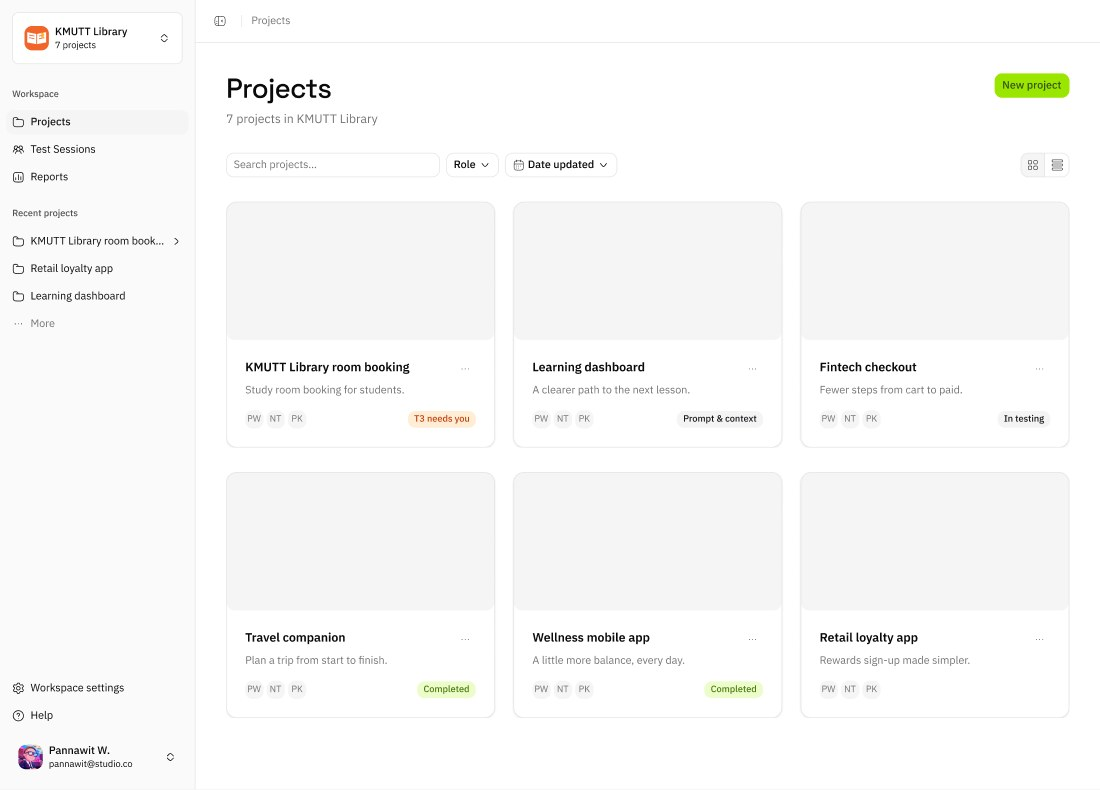
\includegraphics[width=0.48\linewidth,height=5.6cm,keepaspectratio]{figures/ch3-methodology/ui/d10-projects.jpg}}\hfill
  \subfloat[12 Design intent]{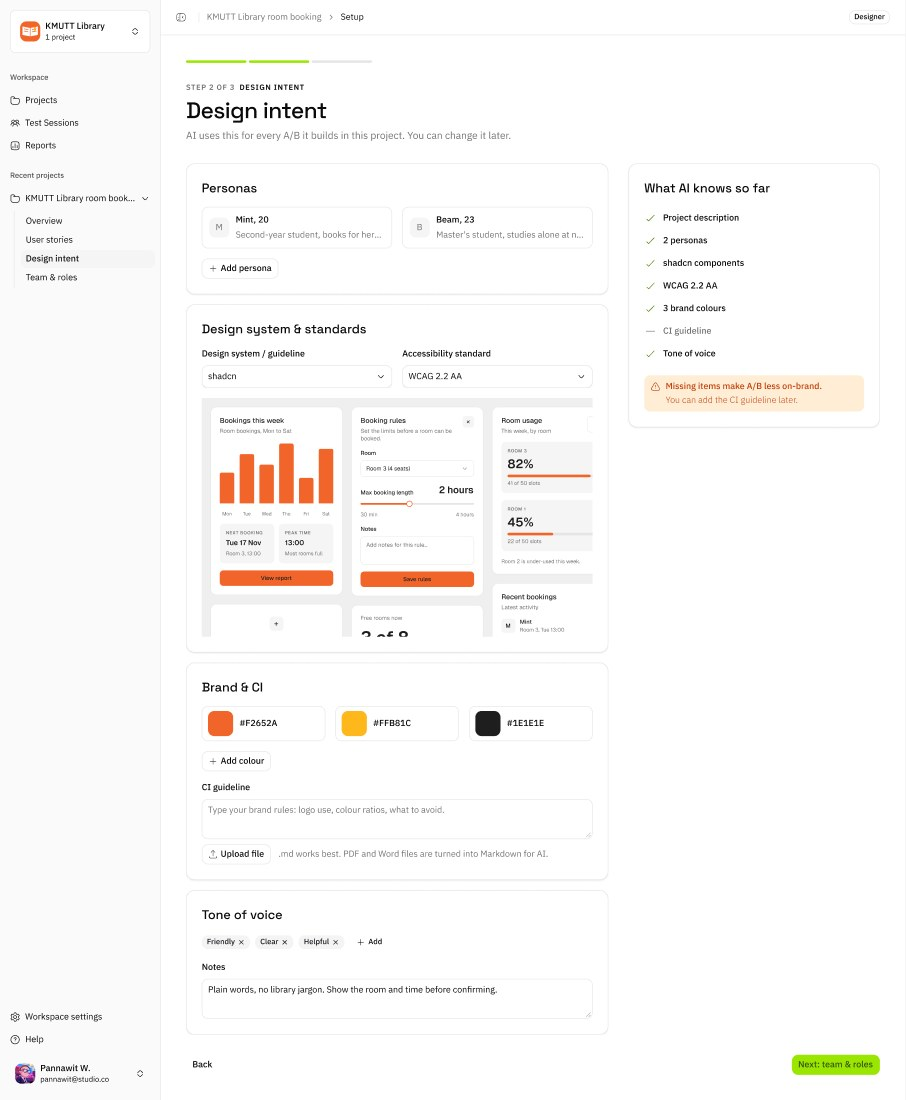
\includegraphics[width=0.48\linewidth,height=5.6cm,keepaspectratio]{figures/ch3-methodology/ui/d12-design-intent.jpg}}\\
  \subfloat[15 User story และ problem statement]{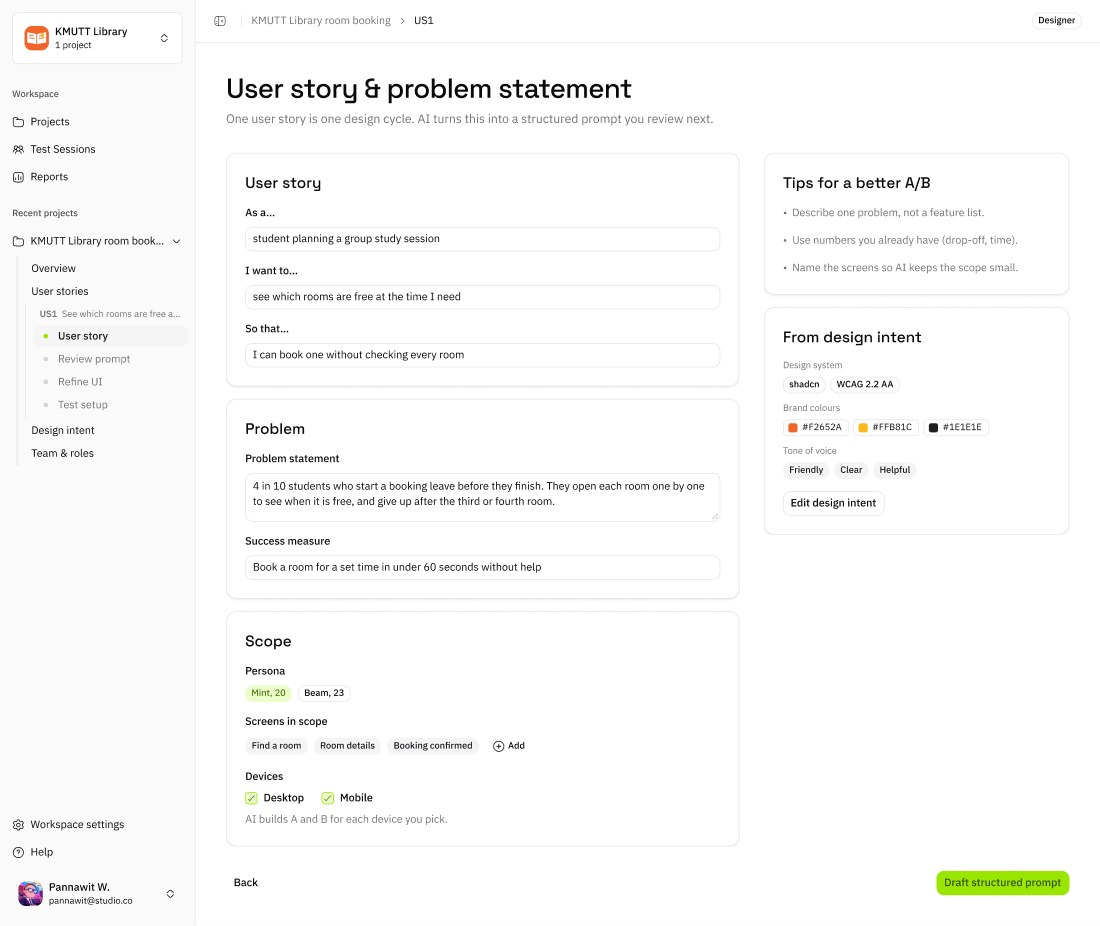
\includegraphics[width=0.48\linewidth,height=5.6cm,keepaspectratio]{figures/ch3-methodology/ui/d15-user-story.jpg}}\hfill
  \subfloat[16 Review structured prompt]{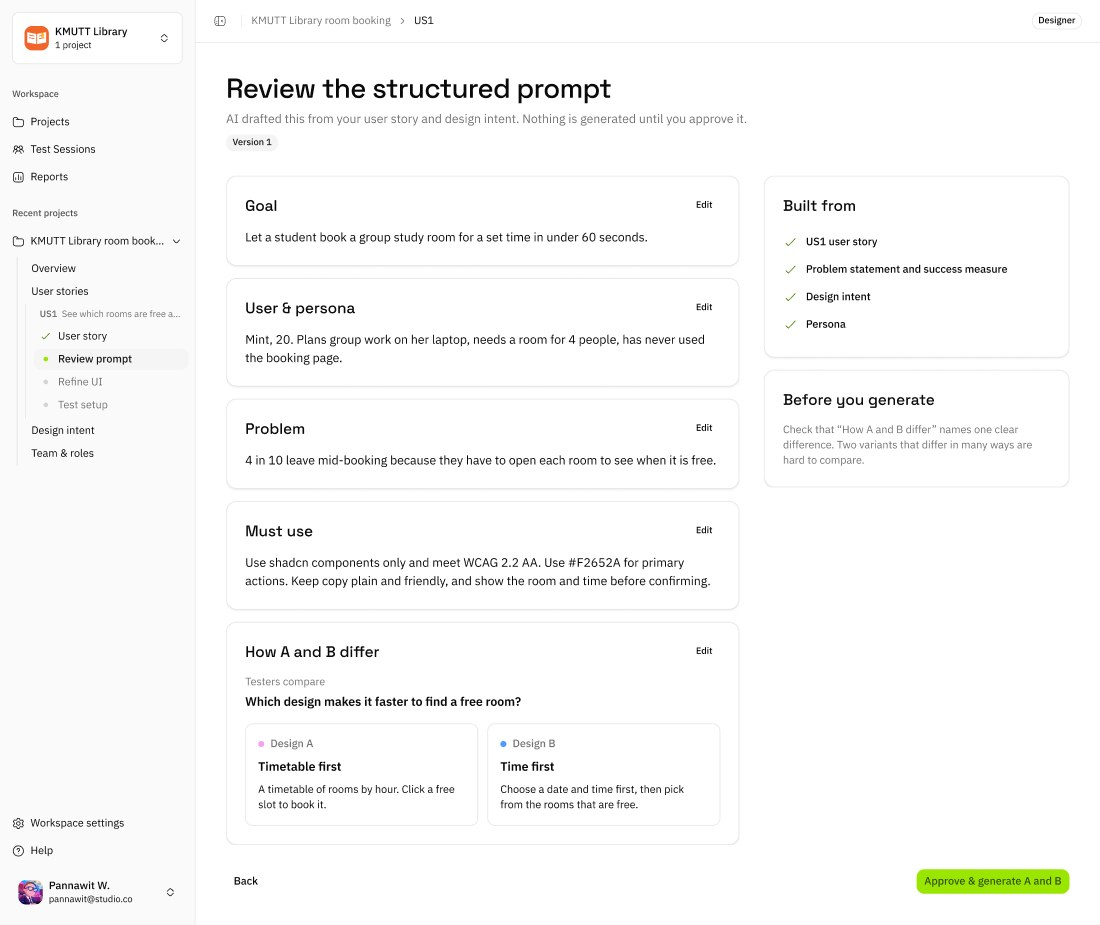
\includegraphics[width=0.48\linewidth,height=5.6cm,keepaspectratio]{figures/ch3-methodology/ui/d16-review-prompt.jpg}}\\
  \subfloat[17 Generating A/B]{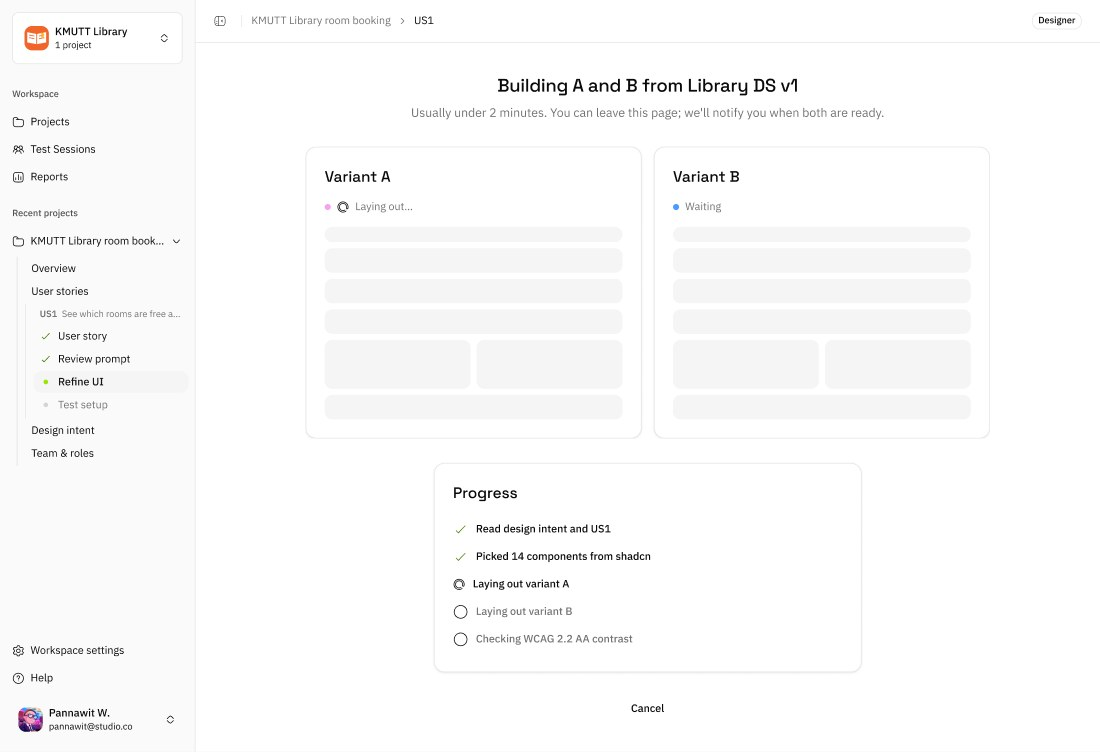
\includegraphics[width=0.48\linewidth,height=5.6cm,keepaspectratio]{figures/ch3-methodology/ui/d17-generating.jpg}}\hfill
  \subfloat[18 Refine A/B]{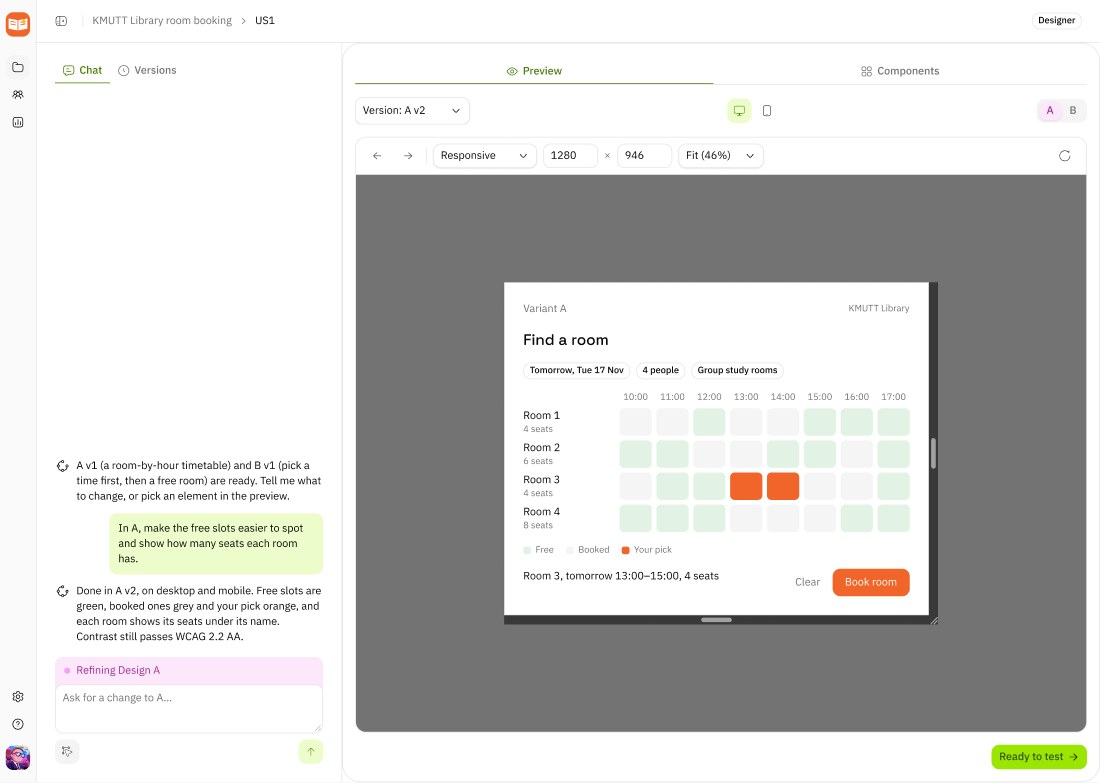
\includegraphics[width=0.48\linewidth,height=5.6cm,keepaspectratio]{figures/ch3-methodology/ui/d18-refine.jpg}}\\
  \caption{Prototype ของ Designer: การตั้งค่าโปรเจกต์และการสร้าง UI ด้วย AI}
  \label{fig:ui-designer-cycle}
\end{figure}
\begin{figure}[H]
  \centering
  \subfloat[19 Test setup]{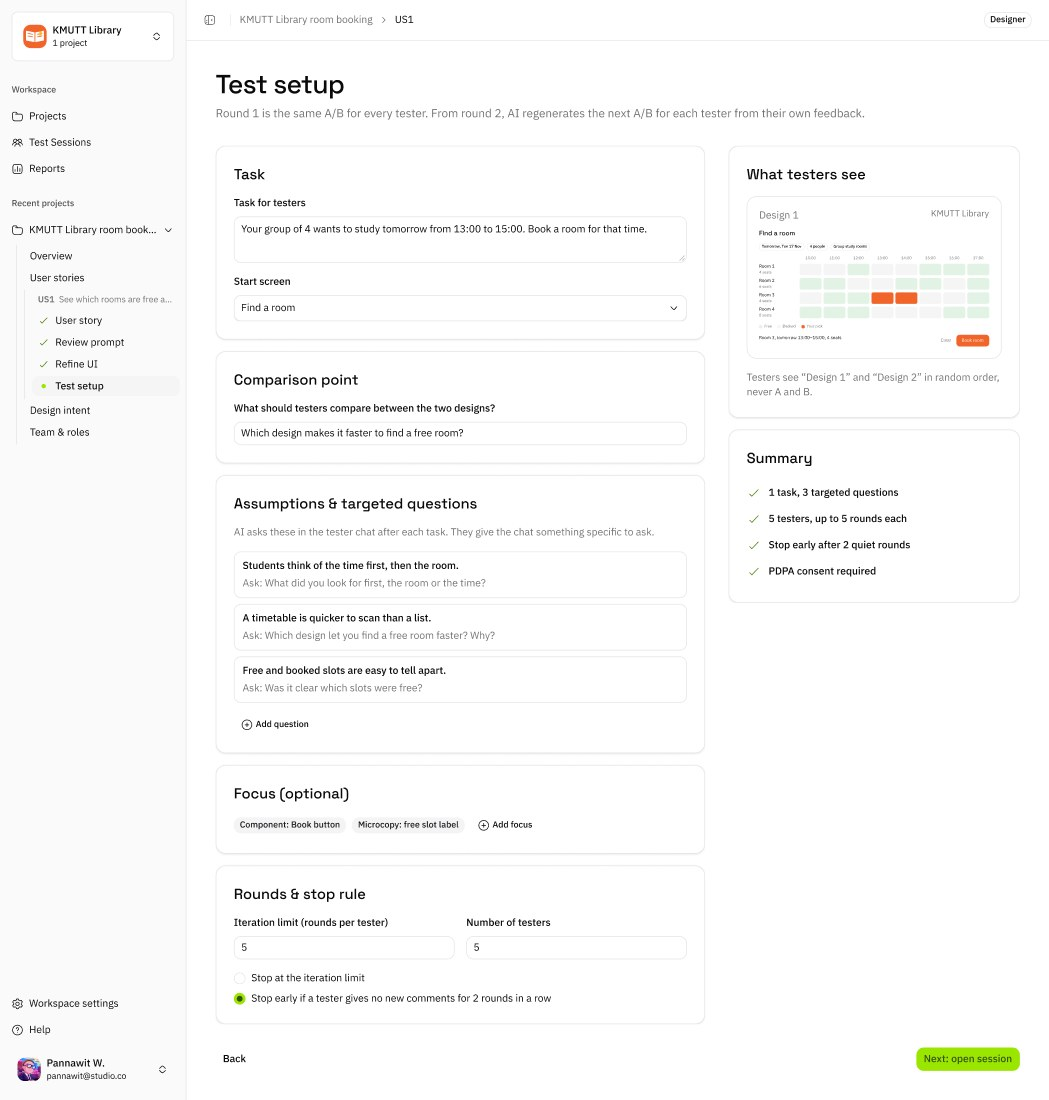
\includegraphics[width=0.48\linewidth,height=5.6cm,keepaspectratio]{figures/ch3-methodology/ui/d19-test-setup.jpg}}\hfill
  \subfloat[21 Monitor testers]{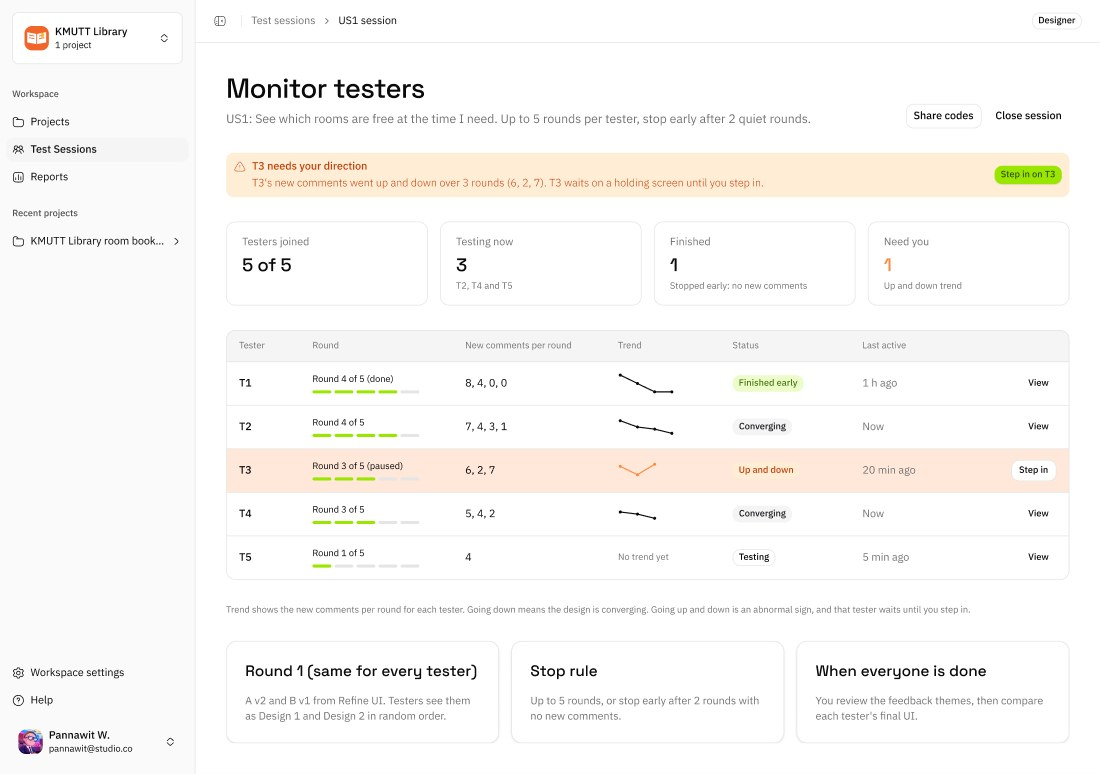
\includegraphics[width=0.48\linewidth,height=5.6cm,keepaspectratio]{figures/ch3-methodology/ui/d21-monitor.jpg}}\\
  \subfloat[23 Review feedback themes]{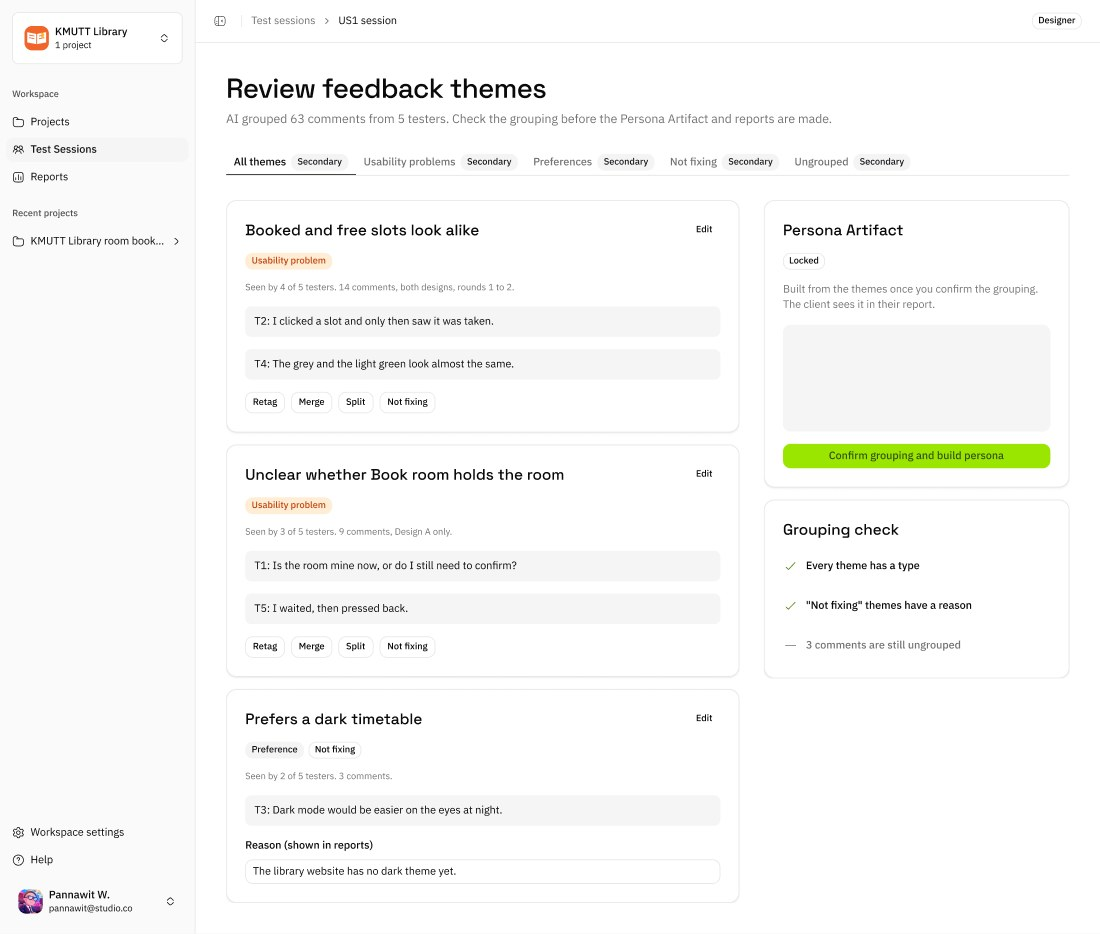
\includegraphics[width=0.48\linewidth,height=5.6cm,keepaspectratio]{figures/ch3-methodology/ui/d23-themes.jpg}}\hfill
  \subfloat[25 Role reports]{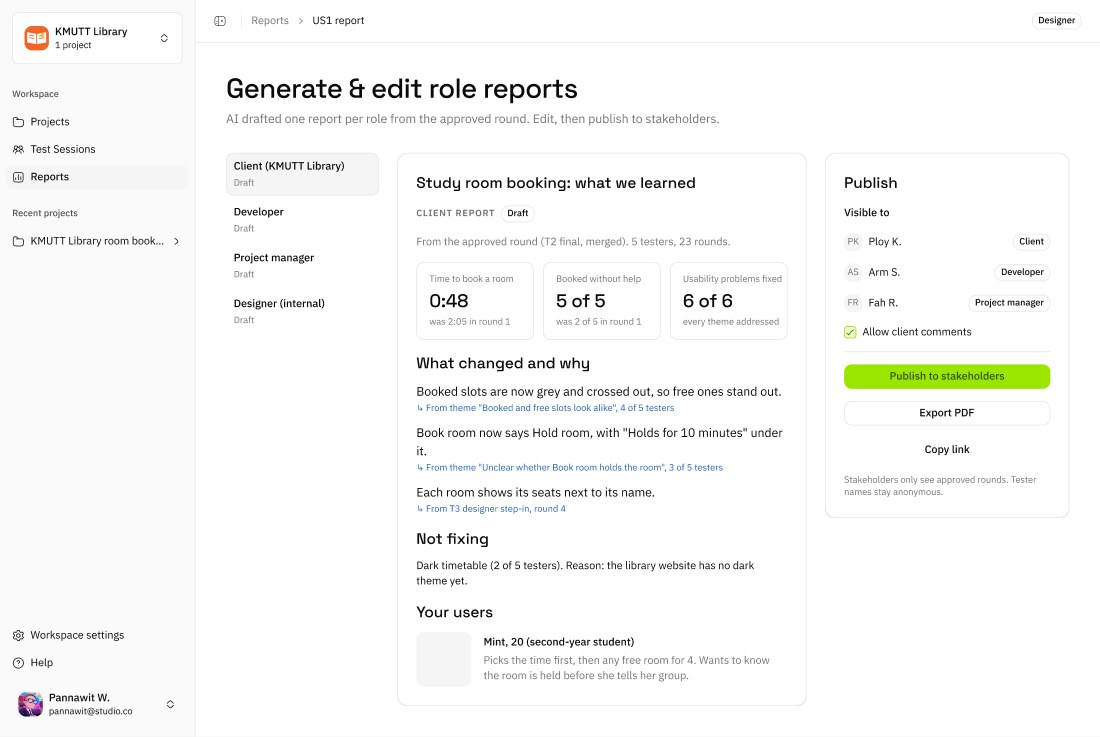
\includegraphics[width=0.48\linewidth,height=5.6cm,keepaspectratio]{figures/ch3-methodology/ui/d25-role-reports.jpg}}\\
  \caption{Prototype ของ Designer: การทดสอบ การวิเคราะห์ข้อเสนอแนะ และรายงาน}
  \label{fig:ui-designer-testing}
\end{figure}
\begin{figure}[H]
  \centering
  \subfloat[27 Consent (PDPA)]{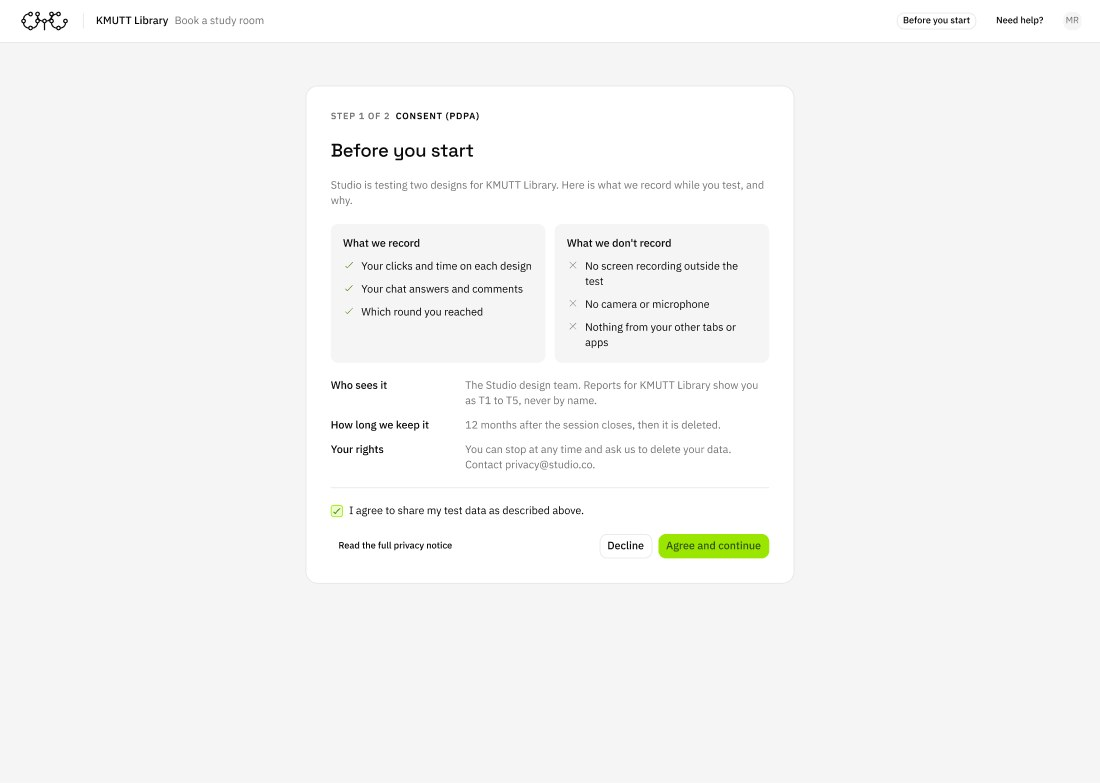
\includegraphics[width=0.48\linewidth,height=5.6cm,keepaspectratio]{figures/ch3-methodology/ui/t27-consent.jpg}}\hfill
  \subfloat[29 Task on Design 1 and 2]{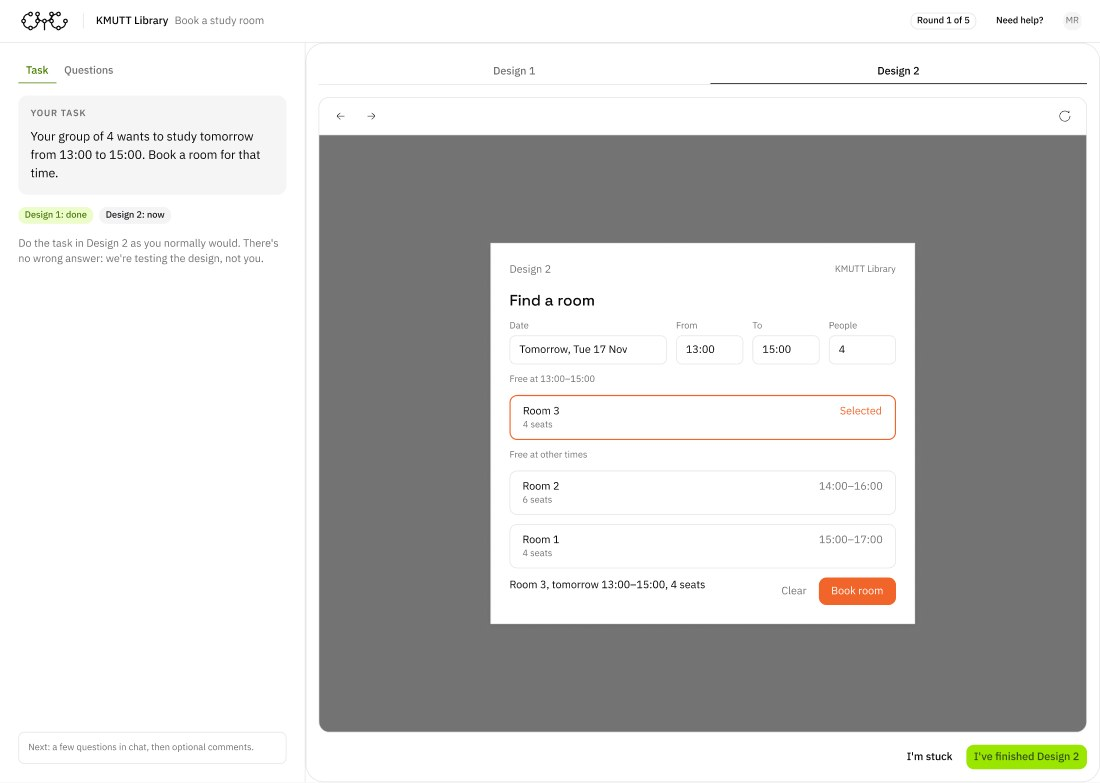
\includegraphics[width=0.48\linewidth,height=5.6cm,keepaspectratio]{figures/ch3-methodology/ui/t29-task.jpg}}\\
  \subfloat[30 Chat feedback]{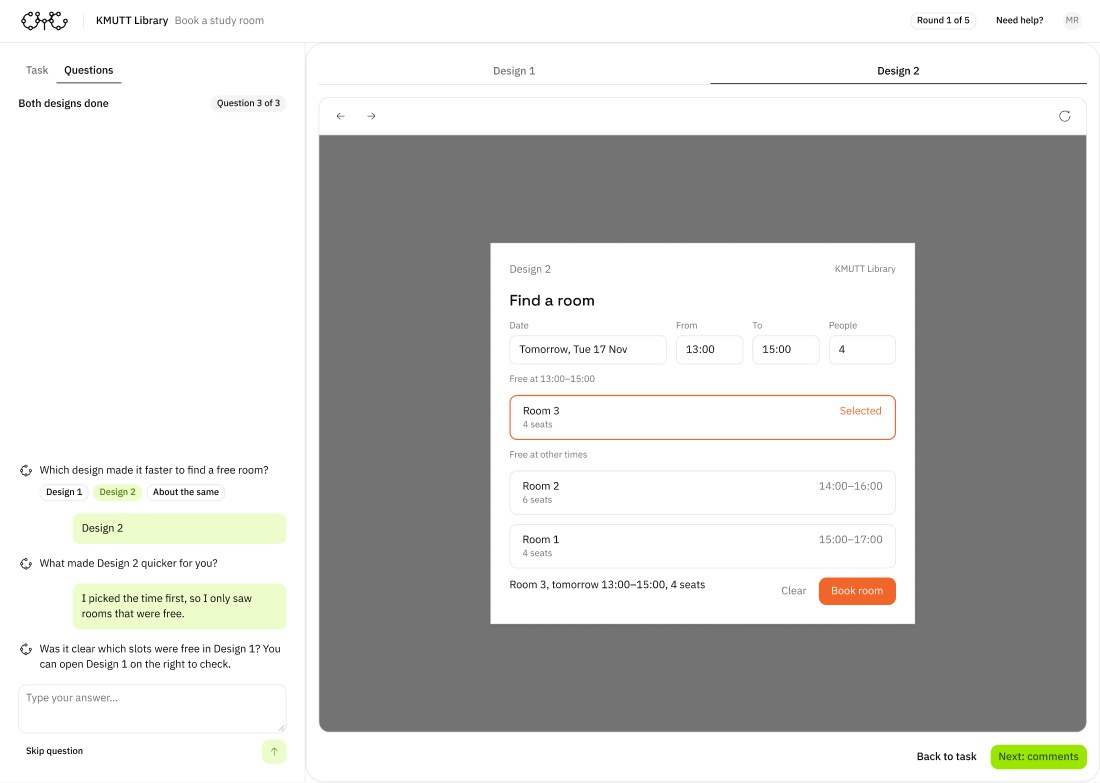
\includegraphics[width=0.48\linewidth,height=5.6cm,keepaspectratio]{figures/ch3-methodology/ui/t30-chat.jpg}}\hfill
  \subfloat[31 Pin a part and comment]{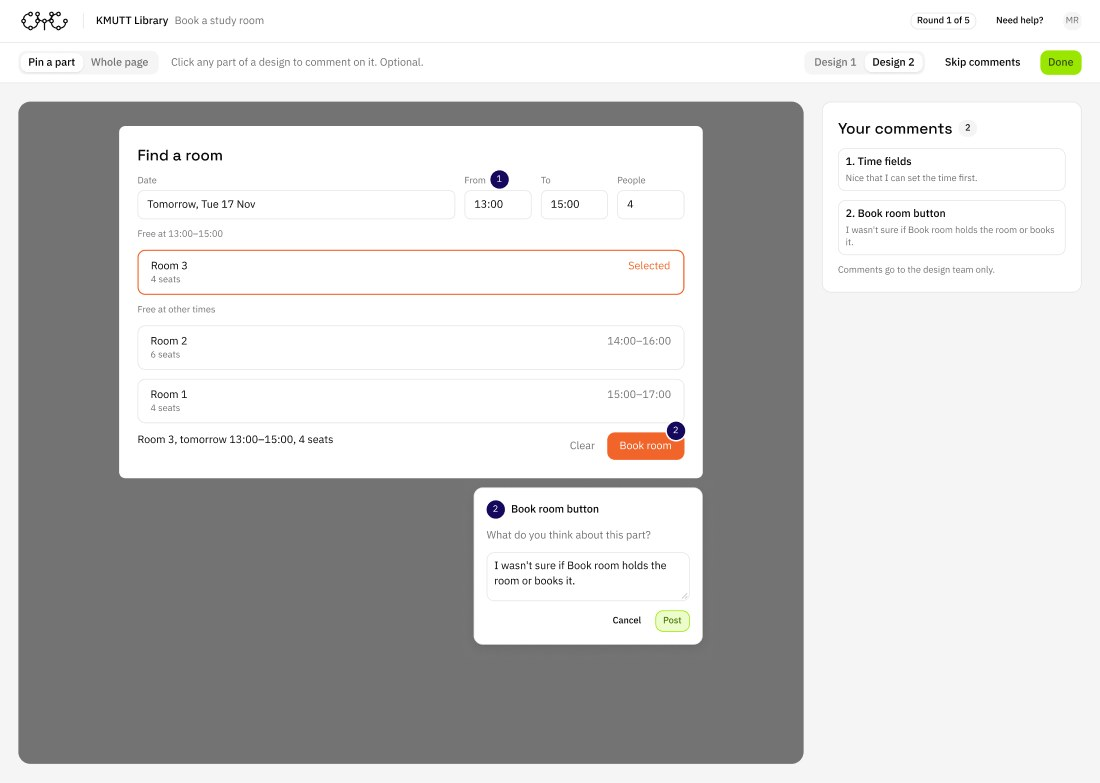
\includegraphics[width=0.48\linewidth,height=5.6cm,keepaspectratio]{figures/ch3-methodology/ui/t31-pin.jpg}}\\
  \caption{Prototype ของ Usability Tester}
  \label{fig:ui-tester}
\end{figure}
\begin{figure}[H]
  \centering
  \subfloat[37 Client report]{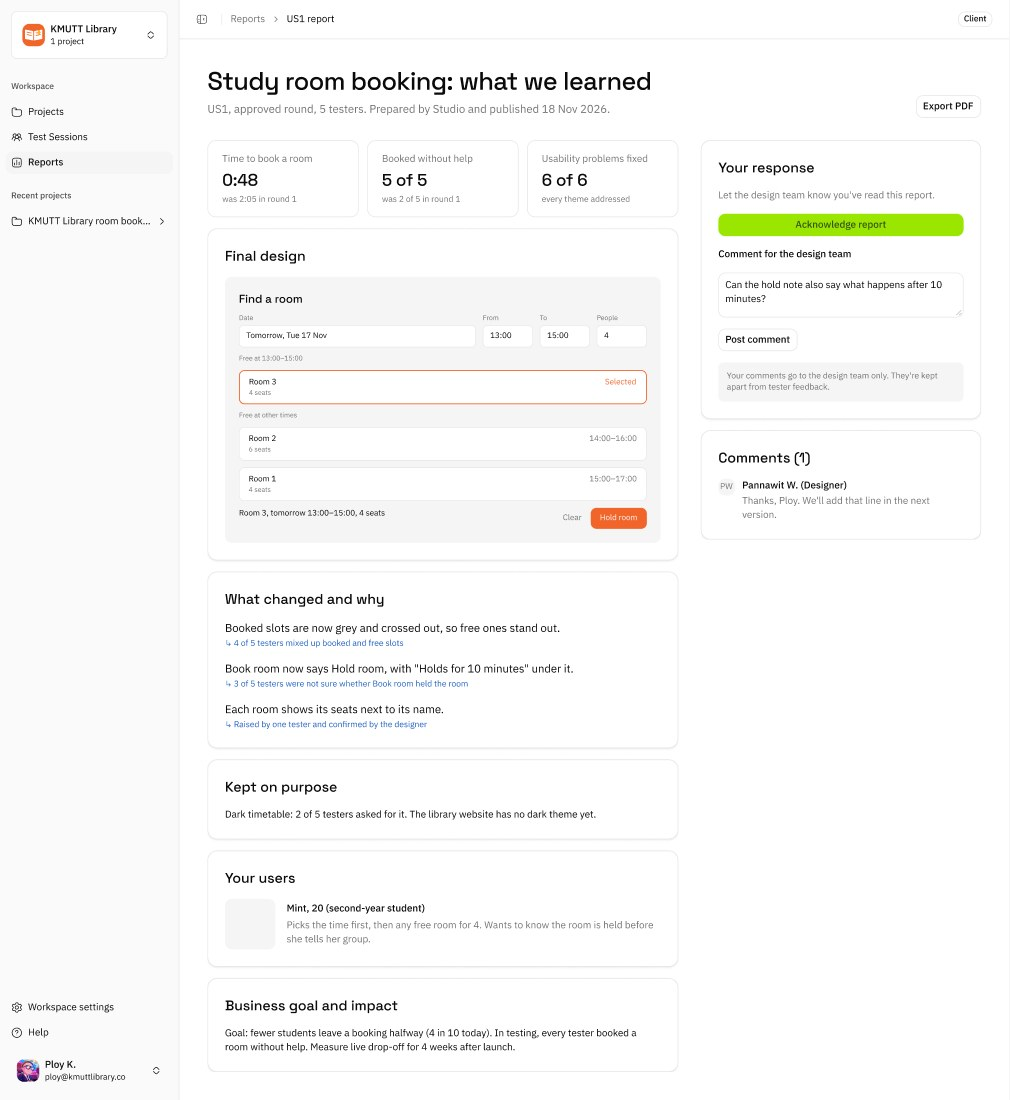
\includegraphics[width=0.48\linewidth,height=7cm,keepaspectratio]{figures/ch3-methodology/ui/s37-client.jpg}}\hfill
  \subfloat[38 Developer handoff]{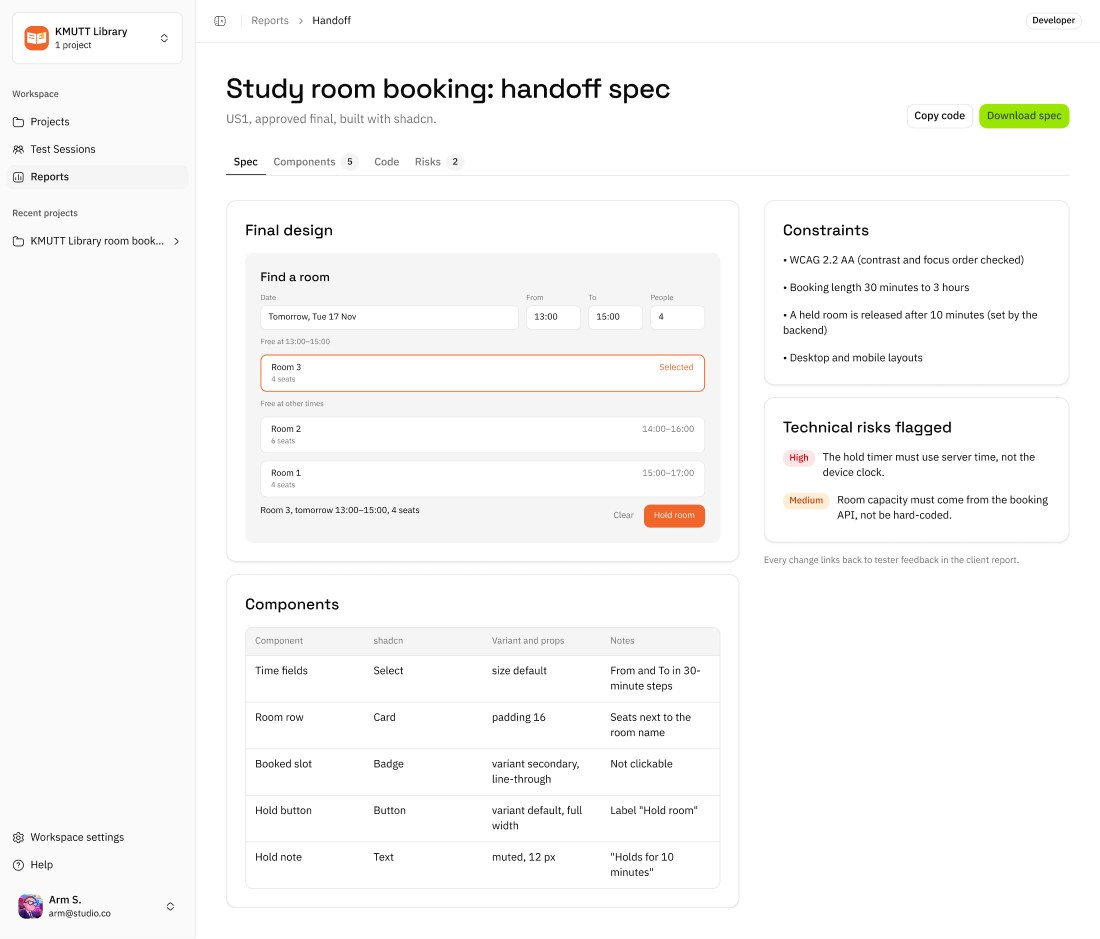
\includegraphics[width=0.48\linewidth,height=7cm,keepaspectratio]{figures/ch3-methodology/ui/s38-developer.jpg}}\\
  \subfloat[39 PM round progress]{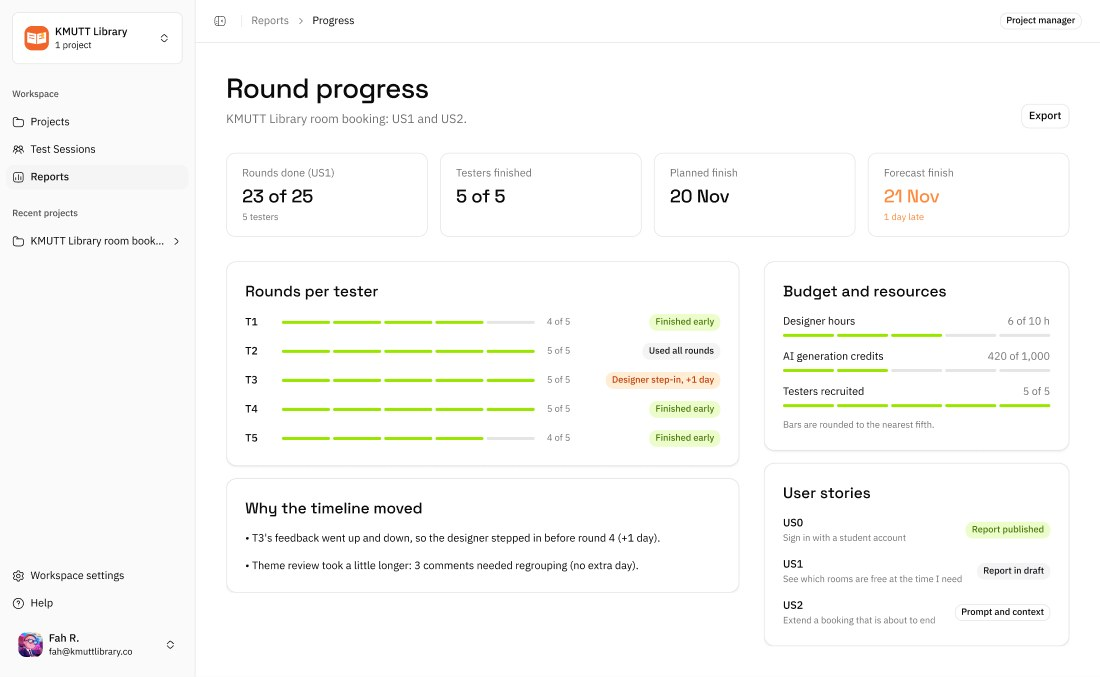
\includegraphics[width=0.48\linewidth,height=7cm,keepaspectratio]{figures/ch3-methodology/ui/s39-pm.jpg}}\\
  \caption{Prototype ของ Client, Developer และ Project Manager}
  \label{fig:ui-stakeholder}
\end{figure}



\end{document}
